% =====================================================================
%  Fondamenti di Unreal Engine, lezione 1 — Introduzione a Unreal
%  Engine: che cos'è un game engine, come si arriva a un'immagine sullo
%  schermo, chi usa l'engine in una produzione, da che cosa è formato un
%  gioco, e il primo contatto con l'editor.
%  Prima lezione del corso breve di introduzione a Unreal Engine (focus
%  sui Blueprints), online su Zoom, dalle 17 alle 19 circa, condotta da
%  Igor, ex studente di game design ed ex level designer di Steel Seed.
%  Contenuti, nell'ordine della lezione: presentazioni; software e game
%  engine; scripting e Blueprint; il rendering 3D (poligoni, vertex
%  shading, rasterizzazione, fragment shading, UV); il real time
%  rendering e i frame; Unreal Engine, i suoi giochi, la prototipazione
%  e il caso Expedition 33; gli engine proprietari di una volta; Unreal
%  nel cinema; il game loop; la produzione (pre-produzione, indie, AA,
%  AAA, outsourcing) e i ruoli che toccano l'engine; l'attività in
%  classe "da che cosa è formato un gioco" (attori, meccaniche, spazi,
%  obiettivi, regole, tempo; MDA); le domande prima della pausa (il
%  tempo come regola, il bilanciamento e il QA, The Midnight Walk e la
%  stop motion, il tempismo delle uscite); il download della 5.5; dopo
%  la pausa le risorse (documentazione, learning, Fab, materiale
%  didattico); un po' di teoria (Play in Editor, delta seconds); il
%  Project Browser e i template; l'interfaccia dell'editor; il
%  transform, gli assi, lo snapping, la navigazione, duplicare,
%  raggruppare, l'Outliner; l'esercitazione dei tre tavoli; il
%  salvataggio e la chiusura.
%  Fonte: trascrizione automatica della prima lezione (UE1), circa due
%  ore. Integrazioni dal libro "Blueprints Visual Scripting for Unreal
%  Engine 5" (Romero, Sewell), segnalate come approfondimenti.
%
%  Pacchetti richiesti nel preambolo del libro (già presenti nel
%  main.tex): \usepackage{booktabs}, \usepackage{tikz} con
%    \usetikzlibrary{shapes.geometric,shapes.symbols,shapes.misc,
%      arrows.meta,positioning,calc,fit}
%  (le librerie vanno caricate nel preambolo, non nel capitolo).
%  Consigliati, come per gli altri capitoli: \usepackage[italian]{babel}
%  e \usepackage[T1]{fontenc} (il capitolo compila anche senza).
%
%  Collocazione nel libro: parte "Fondamenti di Unreal Engine", primo
%  capitolo (numerazione propria 1.1). Nel file principale del libro,
%  subito dopo il \part e il \setcounter della parte:
%
%    % =====================================================================
%  Fondamenti di Unreal Engine, lezione 1 — Introduzione a Unreal
%  Engine: che cos'è un game engine, come si arriva a un'immagine sullo
%  schermo, chi usa l'engine in una produzione, da che cosa è formato un
%  gioco, e il primo contatto con l'editor.
%  Prima lezione del corso breve di introduzione a Unreal Engine (focus
%  sui Blueprints), online su Zoom, dalle 17 alle 19 circa, condotta da
%  Igor, ex studente di game design ed ex level designer di Steel Seed.
%  Contenuti, nell'ordine della lezione: presentazioni; software e game
%  engine; scripting e Blueprint; il rendering 3D (poligoni, vertex
%  shading, rasterizzazione, fragment shading, UV); il real time
%  rendering e i frame; Unreal Engine, i suoi giochi, la prototipazione
%  e il caso Expedition 33; gli engine proprietari di una volta; Unreal
%  nel cinema; il game loop; la produzione (pre-produzione, indie, AA,
%  AAA, outsourcing) e i ruoli che toccano l'engine; l'attività in
%  classe "da che cosa è formato un gioco" (attori, meccaniche, spazi,
%  obiettivi, regole, tempo; MDA); le domande prima della pausa (il
%  tempo come regola, il bilanciamento e il QA, The Midnight Walk e la
%  stop motion, il tempismo delle uscite); il download della 5.5; dopo
%  la pausa le risorse (documentazione, learning, Fab, materiale
%  didattico); un po' di teoria (Play in Editor, delta seconds); il
%  Project Browser e i template; l'interfaccia dell'editor; il
%  transform, gli assi, lo snapping, la navigazione, duplicare,
%  raggruppare, l'Outliner; l'esercitazione dei tre tavoli; il
%  salvataggio e la chiusura.
%  Fonte: trascrizione automatica della prima lezione (UE1), circa due
%  ore. Integrazioni dal libro "Blueprints Visual Scripting for Unreal
%  Engine 5" (Romero, Sewell), segnalate come approfondimenti.
%
%  Pacchetti richiesti nel preambolo del libro (già presenti nel
%  main.tex): \usepackage{booktabs}, \usepackage{tikz} con
%    \usetikzlibrary{shapes.geometric,shapes.symbols,shapes.misc,
%      arrows.meta,positioning,calc,fit}
%  (le librerie vanno caricate nel preambolo, non nel capitolo).
%  Consigliati, come per gli altri capitoli: \usepackage[italian]{babel}
%  e \usepackage[T1]{fontenc} (il capitolo compila anche senza).
%
%  Collocazione nel libro: parte "Fondamenti di Unreal Engine", primo
%  capitolo (numerazione propria 1.1). Nel file principale del libro,
%  subito dopo il \part e il \setcounter della parte:
%
%    % =====================================================================
%  Fondamenti di Unreal Engine, lezione 1 — Introduzione a Unreal
%  Engine: che cos'è un game engine, come si arriva a un'immagine sullo
%  schermo, chi usa l'engine in una produzione, da che cosa è formato un
%  gioco, e il primo contatto con l'editor.
%  Prima lezione del corso breve di introduzione a Unreal Engine (focus
%  sui Blueprints), online su Zoom, dalle 17 alle 19 circa, condotta da
%  Igor, ex studente di game design ed ex level designer di Steel Seed.
%  Contenuti, nell'ordine della lezione: presentazioni; software e game
%  engine; scripting e Blueprint; il rendering 3D (poligoni, vertex
%  shading, rasterizzazione, fragment shading, UV); il real time
%  rendering e i frame; Unreal Engine, i suoi giochi, la prototipazione
%  e il caso Expedition 33; gli engine proprietari di una volta; Unreal
%  nel cinema; il game loop; la produzione (pre-produzione, indie, AA,
%  AAA, outsourcing) e i ruoli che toccano l'engine; l'attività in
%  classe "da che cosa è formato un gioco" (attori, meccaniche, spazi,
%  obiettivi, regole, tempo; MDA); le domande prima della pausa (il
%  tempo come regola, il bilanciamento e il QA, The Midnight Walk e la
%  stop motion, il tempismo delle uscite); il download della 5.5; dopo
%  la pausa le risorse (documentazione, learning, Fab, materiale
%  didattico); un po' di teoria (Play in Editor, delta seconds); il
%  Project Browser e i template; l'interfaccia dell'editor; il
%  transform, gli assi, lo snapping, la navigazione, duplicare,
%  raggruppare, l'Outliner; l'esercitazione dei tre tavoli; il
%  salvataggio e la chiusura.
%  Fonte: trascrizione automatica della prima lezione (UE1), circa due
%  ore. Integrazioni dal libro "Blueprints Visual Scripting for Unreal
%  Engine 5" (Romero, Sewell), segnalate come approfondimenti.
%
%  Pacchetti richiesti nel preambolo del libro (già presenti nel
%  main.tex): \usepackage{booktabs}, \usepackage{tikz} con
%    \usetikzlibrary{shapes.geometric,shapes.symbols,shapes.misc,
%      arrows.meta,positioning,calc,fit}
%  (le librerie vanno caricate nel preambolo, non nel capitolo).
%  Consigliati, come per gli altri capitoli: \usepackage[italian]{babel}
%  e \usepackage[T1]{fontenc} (il capitolo compila anche senza).
%
%  Collocazione nel libro: parte "Fondamenti di Unreal Engine", primo
%  capitolo (numerazione propria 1.1). Nel file principale del libro,
%  subito dopo il \part e il \setcounter della parte:
%
%    % =====================================================================
%  Fondamenti di Unreal Engine, lezione 1 — Introduzione a Unreal
%  Engine: che cos'è un game engine, come si arriva a un'immagine sullo
%  schermo, chi usa l'engine in una produzione, da che cosa è formato un
%  gioco, e il primo contatto con l'editor.
%  Prima lezione del corso breve di introduzione a Unreal Engine (focus
%  sui Blueprints), online su Zoom, dalle 17 alle 19 circa, condotta da
%  Igor, ex studente di game design ed ex level designer di Steel Seed.
%  Contenuti, nell'ordine della lezione: presentazioni; software e game
%  engine; scripting e Blueprint; il rendering 3D (poligoni, vertex
%  shading, rasterizzazione, fragment shading, UV); il real time
%  rendering e i frame; Unreal Engine, i suoi giochi, la prototipazione
%  e il caso Expedition 33; gli engine proprietari di una volta; Unreal
%  nel cinema; il game loop; la produzione (pre-produzione, indie, AA,
%  AAA, outsourcing) e i ruoli che toccano l'engine; l'attività in
%  classe "da che cosa è formato un gioco" (attori, meccaniche, spazi,
%  obiettivi, regole, tempo; MDA); le domande prima della pausa (il
%  tempo come regola, il bilanciamento e il QA, The Midnight Walk e la
%  stop motion, il tempismo delle uscite); il download della 5.5; dopo
%  la pausa le risorse (documentazione, learning, Fab, materiale
%  didattico); un po' di teoria (Play in Editor, delta seconds); il
%  Project Browser e i template; l'interfaccia dell'editor; il
%  transform, gli assi, lo snapping, la navigazione, duplicare,
%  raggruppare, l'Outliner; l'esercitazione dei tre tavoli; il
%  salvataggio e la chiusura.
%  Fonte: trascrizione automatica della prima lezione (UE1), circa due
%  ore. Integrazioni dal libro "Blueprints Visual Scripting for Unreal
%  Engine 5" (Romero, Sewell), segnalate come approfondimenti.
%
%  Pacchetti richiesti nel preambolo del libro (già presenti nel
%  main.tex): \usepackage{booktabs}, \usepackage{tikz} con
%    \usetikzlibrary{shapes.geometric,shapes.symbols,shapes.misc,
%      arrows.meta,positioning,calc,fit}
%  (le librerie vanno caricate nel preambolo, non nel capitolo).
%  Consigliati, come per gli altri capitoli: \usepackage[italian]{babel}
%  e \usepackage[T1]{fontenc} (il capitolo compila anche senza).
%
%  Collocazione nel libro: parte "Fondamenti di Unreal Engine", primo
%  capitolo (numerazione propria 1.1). Nel file principale del libro,
%  subito dopo il \part e il \setcounter della parte:
%
%    \input{UE/UE1_introduzione_a_unreal_engine}
%
%  Tutte le etichette di questo capitolo hanno il prefisso "ue1:"
%  (ue1:cap:..., ue1:sec:..., ue1:fig:..., ue1:tab:...), e tutti gli
%  stili TikZ hanno il prefisso "ue1" (ue1box, ue1arr, ...) per non
%  collidere con chiavi native di TikZ. Il capitolo è autonomo: non
%  contiene \ref verso altri capitoli.
%  Le figure sono ricostruzioni schematiche di quanto mostrato e detto a
%  lezione, non copie delle slide del docente. Dove la trascrizione è
%  troppo rovinata per ricostruire un dettaglio, il capitolo lo dice
%  invece di inventarlo.
% =====================================================================

\chapter[Introduzione a Unreal Engine]{Introduzione a Unreal Engine: che cos'è un
engine, chi lo usa, e il primo contatto con l'editor}
\label{ue1:cap:intro}

Questa è la \textbf{prima lezione} del corso breve di \textbf{introduzione a Unreal
Engine}, un corso che ha il suo centro nei \textbf{Blueprint}, il sistema di
programmazione visuale ``a nodi'' dell'engine di Epic Games. La lezione ha due metà
molto diverse. La prima è teorica e larga: che cos'è un \emph{software}, che cos'è un
\emph{game engine}, come un modello fatto di poligoni diventa un'immagine sullo
schermo, perché Unreal è oggi l'engine più diffuso, quali figure di una produzione lo
usano e per che cosa, e infine, con un'attività in classe, da che cosa è formato un
gioco. La seconda metà è pratica: si scarica Unreal Engine 5.5, si guardano le risorse
che Epic mette a disposizione (la documentazione, i corsi gratuiti, il negozio di
\emph{asset} Fab), si crea un primo progetto vuoto e si impara a muoversi nell'editor:
piazzare un cubo, spostarlo, ruotarlo, scalarlo, duplicarlo, raggrupparlo, ordinarlo
in cartelle. La lezione si chiude con un'esercitazione: arredare un piccolo
ristorante con tre tavoli e le loro sedie.

Il docente è \textbf{Igor}\footnote{Il docente si presenta come ``Igor Ripanti''; il
cognome è quello della trascrizione automatica, che altrove storpia quasi tutti i nomi
propri, e il capitolo non è in grado di verificarlo.}, che si presenta come ex alunno
della stessa scuola degli studenti, ``precisamente per quanto riguarda game
design''\footnote{La trascrizione dice ``sono stato un alunno di Live'': il nome della
scuola è con ogni probabilità storpiato.}. Ha lavorato a \textbf{\emph{Steel Seed}},
``principalmente come \emph{level designer}''; ma ``essendo un ambiente indie'' faceva
``un po' di tutto'', anche programmazione e \emph{scripting}, e quindi ha fatto ``uso
intensivo'' di Unreal Engine ``e di tutte le sue feature''. Il corso è diviso tra due
docenti: con Igor la parte di programmazione e di ``piccole feature''; con
\textbf{Davide}, a partire dal 26 del mese, una parte ``un po' più artistica''. Le
lezioni si alternano: il giovedì successivo gli studenti saranno di nuovo con Igor, il
martedì dopo con Davide.

La lezione è \textbf{online}, su Zoom, con un server Discord del corso per i
materiali e le domande; inizia poco dopo le 17 e finisce alle 19, con una pausa di una
decina di minuti verso le 17 e mezza\footnote{Igor, credendo per errore che la lezione
finisse alle 18 (``sono da un altro corso che finiva alle 18''), dopo la pausa annuncia
che ``manca mezz'ora alla fine''; gli studenti lo correggono (``nella mail c'era
scritto'' alle 19), e il docente ha ``un'altra ora'' per la parte pratica.}. Gli
studenti sono tutti \textbf{nuovi iscritti al primo anno}, di corsi diversi: game
design (la maggioranza), narrative design, character animation, 3D art e
programmazione. Il corso breve, in altre parole, è comune a figure che in una
produzione useranno Unreal in modi molto diversi, ed è proprio da questa varietà che
Igor parte.

Tre avvertenze di lettura. La prima: la trascrizione è automatica e storpia moltissimi
nomi. Unreal diventa ``Arreal'', ``Arial Engine'', ``ArrayLange'', ``ArrayLab'',
``Arrival Engine'', ``Arrial'', ``Ariane Engine'', ``Riala'' e ``a Real Engine'';
\emph{Clair Obscur: Expedition 33} è ``Expedition'' e ``Spedisce 33''; Sandfall
Interactive è ``Send Follow Interactive''; \emph{shader} è anche ``scender''. Dove la
ricostruzione è sicura il capitolo usa la forma corretta e, la prima volta, lo segnala
in nota; dove non lo è riporta la forma della trascrizione e lo dice. La seconda: in
più punti la registrazione contiene lunghi blocchi di testo senza senso e ripetuto
(``qual è la risposta che ci può essere?'', ``a parte il plus time\ldots''): sono
artefatti del riconoscimento vocale durante la pausa e i momenti di lavoro
individuale, e il capitolo li ignora. La terza: la seconda metà della lezione è una
dimostrazione dal vivo nell'editor; il capitolo ricostruisce i passaggi da ciò che Igor
dice mentre li fa, e li completa, dove serve, con i nomi esatti dei comandi.

\paragraph{Come leggere questo capitolo.} Il capitolo segue l'ordine della lezione.
Le figure ricostruiscono gli schemi spiegati a voce o sulle slide (la pipeline di
rendering, il \emph{game loop}, gli elementi di un gioco, l'interfaccia dell'editor,
il \emph{transform}); le tabelle riassumono i ruoli della produzione e le scorciatoie
da tastiera della seconda parte. Qua e là, dei paragrafi di \textbf{approfondimento}
collegano la lezione al libro \emph{Blueprints Visual Scripting for Unreal Engine 5}
di Marcos Romero e Brenden Sewell, che sarà il testo di riferimento per questa parte
del libro, e a qualche nozione tecnica generale; sono segnalati come tali e non fanno
parte della lezione.

Il percorso del capitolo:
\begin{enumerate}
  \item le presentazioni e le esperienze degli studenti (sezione
        \ref{ue1:sec:presentazioni});
  \item il \textbf{software}, il \textbf{game engine} e lo \textbf{scripting}, con i
        Blueprint (sezione \ref{ue1:sec:engine});
  \item il \textbf{rendering 3D}: poligoni, \emph{vertex shading}, rasterizzazione,
        \emph{fragment shading}; poi il \emph{real time rendering} e i \emph{frame}
        (sezioni \ref{ue1:sec:rendering} e~\ref{ue1:sec:realtime});
  \item \textbf{Unreal Engine}: perché è così usato, la prototipazione, i giochi, gli
        engine di una volta, il cinema, il \textbf{game loop} (sezioni
        da~\ref{ue1:sec:unreal} a~\ref{ue1:sec:gameloop});
  \item la \textbf{produzione} e i \textbf{ruoli} che toccano l'engine (sezioni
        \ref{ue1:sec:produzione} e~\ref{ue1:sec:ruoli});
  \item l'attività in classe: \textbf{da che cosa è formato un gioco}, e le domande
        prima della pausa (sezioni \ref{ue1:sec:elementi} e~\ref{ue1:sec:domande});
  \item il \textbf{download} della 5.5, le \textbf{risorse} (documentazione,
        \emph{learning}, Fab) e un po' di teoria sul \emph{Play in Editor} e sul
        \emph{delta time} (sezioni da~\ref{ue1:sec:download} a~\ref{ue1:sec:pie});
  \item il primo contatto con l'\textbf{editor}: il progetto, l'interfaccia, il
        \textbf{transform}, la navigazione, l'organizzazione (sezioni
        da~\ref{ue1:sec:progetto} a~\ref{ue1:sec:outliner});
  \item l'\textbf{esercitazione dei tre tavoli}, il salvataggio e la chiusura (sezioni
        \ref{ue1:sec:esercitazione} e~\ref{ue1:sec:chiusura}).
\end{enumerate}

% ---------------------------------------------------------------------
\section{Presentazioni: chi c'è, e chi ha già aperto un engine}
\label{ue1:sec:presentazioni}

La lezione comincia con qualche minuto di attesa (``aspettiamo cinque, dieci minuti''),
un appello e una richiesta: accendere la webcam, ``così almeno ci vediamo un po' in
faccia''. A chi non ha una webcam Igor suggerisce le applicazioni che trasformano il
telefono in una webcam, ``come se ti facessi una videochiamata'': lui usa di solito
\emph{Iriun}\footnote{Nella trascrizione ``Ingur'' e ``Iruin''; si tratta con ogni
probabilità di \emph{Iriun Webcam}, un'applicazione gratuita che fa esattamente
questo.}. I lavori in corso nell'edificio del docente producono ``rumori molesti'' per
tutta la lezione, e Igor se ne scusa.

Poi il giro di presentazioni: nome, corso, ``un piccolo background''. Tutti sono iscritti
al primo anno; i corsi sono game design, character animation, narrative design (più di
uno), 3D art e programmazione. ``C'è una bella quantità di nuovi compagni di design'',
commenta Igor, ``quindi avremo pane per i nostri denti'', oltre ovviamente a 3D art e
programmazione.

\paragraph{Chi ha già usato un engine?} La domanda successiva è se qualcuno abbia ``mai
aperto un software di \emph{develop} per i videogiochi'': Unity, Godot, ``in
generale''. Qualcuno ha provato Godot; qualcuno un po' di Unity, seguendo un corso
online ``molto veloce'' e facendo ``un paio di giochini'', un \emph{platform} e un clone
di \emph{Flappy Bird}, ``di 3D niente''; qualcuno è ``digiuno'', e qualcun altro ha
lavorato ``con roba presa da Fab''. Igor accoglie tutte le risposte allo stesso modo:
``ci sta assolutamente''. Fab, aggiunge, sarà uno dei temi di oggi, perché è ``una
risorsa incredibile'', soprattutto per le cose gratis, quelle in sconto e i contenuti
gratuiti del mese.

\paragraph{La mentalità prima degli strumenti.} A chi parte da zero Igor dà subito una
rassicurazione che vale per tutto il corso: ``l'importante è avere la mentalità''. In
programmazione, ``molto spesso'' si tratta ``semplicemente'' di imparare a usare gli
strumenti, mentre ``la logica fa da padrone''. Passare da un engine all'altro, o da
nessun engine al primo, è soprattutto ``riabituarsi a un nuovo campo di gioco''.

% ---------------------------------------------------------------------
\section{Software, game engine e scripting}
\label{ue1:sec:engine}

\paragraph{Che cos'è un software.} Igor parte dalla definizione più semplice possibile:
il \textbf{software} è ``quello che non è hardware, fondamentalmente''. È un insieme di
istruzioni, di dati e di programmi con funzionalità precise, che ci permettono di
creare cose: strumenti di 3D art come \textbf{Blender} e \textbf{Maya}, oppure
\emph{engine} come \textbf{Unreal Engine} e \textbf{Unity}.

\paragraph{L'engine come calderone.} Il \textbf{game engine} è ``il calderone, chiamiamolo
un po' così'', che riunisce tutte le facoltà di chi sviluppa (3D art, programmazione,
design) e le mette ``in un ambiente comune'', l'ambiente di sviluppo dell'engine. Gli
engine più noti sono \textbf{Unreal}, \textbf{Unity}, \textbf{Godot} e
\textbf{GameMaker}, e ognuno contiene al suo interno molte funzionalità: i
\textbf{motori fisici}, che gestiscono le \textbf{collisioni}; la gestione dei
\textbf{suoni}; le \textbf{animazioni}; il \textbf{networking}; l'\textbf{intelligenza
artificiale} dei personaggi. Nessuna di queste cose ``si fa da sola'': ci mettono le
mani gli sviluppatori, ``tramite lo \emph{scripting}''.

\paragraph{Lo scripting, e i Blueprint.} Lo \textbf{scripting} è ``la forma di
programmazione che ci permette di entrare in interazione e creare cose all'interno
dell'engine''. Esistono molti linguaggi: Igor cita il \textbf{C}, il \textbf{C\#}
(quello di Unity) e i \textbf{Blueprint}, che sono il tipo di \emph{scripting} di Unreal
Engine e l'oggetto di questo corso. Più avanti nella lezione (sezione~\ref{ue1:sec:ruoli})
Igor tornerà sul punto: in Unreal si può programmare anche in codice (in C++), ``ma noi
non lo useremo'', perché i Blueprint bastano ``tranquillamente'', sono usati anche dai
programmatori, e ``tanti giochi nel comparto indie'' sono fatti ``solo con Blueprint,
senza mai toccare una riga di codice''. I Blueprint sono un \textbf{linguaggio a nodi}:
``prendiamo proprio e colleghiamo tutti i nodini'' per dare un senso alla
programmazione.

\paragraph{Approfondimento: le due accezioni di ``Blueprint''.} Romero e Sewell, nel
primo capitolo di \emph{Blueprints Visual Scripting for Unreal Engine 5}, fanno notare
che in Unreal la parola \emph{Blueprint} ha due significati. È il nome del
\textbf{linguaggio di scripting visuale} creato da Epic Games; ed è anche il nome di un
\textbf{tipo di oggetto di gioco} creato con quel linguaggio. I Blueprint di questo
secondo tipo sono di due specie: il \textbf{Level Blueprint}, uno per ogni livello del
gioco (non se ne possono creare altri separati), e le \textbf{Blueprint Class}, che
servono a creare oggetti interattivi riutilizzabili in qualunque livello. Un progetto di
Unreal Engine 5, aggiungono gli autori, si può sviluppare in Blueprint, in C++ o in una
combinazione dei due: si può aggiungere codice C++ a un progetto Blueprint e viceversa.
La scelta di partire dai Blueprint, quindi, non chiude nessuna porta.

% ---------------------------------------------------------------------
\section{Il rendering 3D: dai poligoni ai pixel}
\label{ue1:sec:rendering}

Un'applicazione grafica come un gioco 3D ha una particolarità: il \textbf{3D
rendering}, cioè ``la fase finale dello sviluppo di un'immagine''. È il processo che
prende un \textbf{\emph{3D asset}} (``per il linguaggio un po' più tecnico'') e ci
presenta davanti la scena vera e propria, con gli oggetti creati dai 3D artist ``che
hanno faticato tanto per poterlo fare''. Quegli oggetti sono formati da
\textbf{poligoni}.

\paragraph{Quanti poligoni ha questo oggetto?} Igor chiede se qualcuno ha mai sentito
parlare del numero di poligoni di un modello. Uno studente sì: gli sono capitati ``dei
video di ottimizzazione'' su come diminuire i poligoni ``per cercare di diminuire il
\emph{lag}''. ``Esatto, bravissimo.'' La regola è semplice, e Igor la dice con una
battuta: ``se mai doveste avere il caso fortuito di avere un cubo con due milioni di
poligoni, sappiate che il vostro gioco esploderà, probabilmente''. Nella
\textbf{viewport} (``un elemento che poi vedremo'': la finestra in cui l'engine, ma
anche Blender mentre si modella, mostra la scena) vale sempre lo stesso compromesso:
\textbf{più poligoni ci sono, più l'immagine è precisa, ma più è pesante da
renderizzare}.

\paragraph{Le tre fasi.} Il rendering di un'immagine passa per molti passaggi; ``noi oggi''
ne guardiamo tre principali (figura~\ref{ue1:fig:pipeline}).
\begin{enumerate}
  \item \textbf{\emph{Vertex shading}.} Le immagini e i modelli sono formati
        principalmente da \textbf{triangoli}, e i triangoli sono formati da
        \textbf{vertici}. I vertici definiscono la forma: in questa fase si
        identificano e si posizionano i tre punti di ogni triangolo.
  \item \textbf{Rasterizzazione.} Il triangolo così definito viene
        \emph{rasterizzato}: si stabilisce quali \textbf{pixel} dello schermo cadono
        dentro quel triangolino. Igor la spiega a partire dalla grafica 2D (``qualcuno
        ha fatto grafica?'', e una studentessa laureata in grafica conferma). Un'immagine
        \textbf{raster}, come quelle di Photoshop, è fatta di pixel; un'immagine
        \textbf{vettoriale} è fatta di vettori. La differenza: se si ingrandisce
        (``strecciate'') un'immagine raster, diventa ``sgranatissima''; un'immagine
        vettoriale la si può ingrandire ``quanto volete'' e resta uguale. Gli schermi,
        però, sono fatti di pixel: per questo i triangoli vanno rasterizzati.
  \item \textbf{\emph{Fragment shading}.} È la fase finale, quella ``vicina alla
        visualizzazione''. Ai \textbf{frammenti} (``poligoni, triangoli, chiamateli
        come vi pare'') si applicano i \textbf{colori}, la \textbf{luce}, le
        \textbf{ombreggiature} e i \textbf{riflessi}, tenendo conto della posizione
        della camera. È anche ``una parte molto artistica'', perché Unreal lavora molto
        sulla resa della luce: si possono piazzare luci, gestire come la luce entra in
        una stanza, e così via.
\end{enumerate}

\begin{figure}[htbp]
\centering
\begin{tikzpicture}[
  font=\small,
  ue1box/.style={draw, thick, rounded corners=3pt, minimum height=1.5cm,
               text width=2.6cm, align=center},
  ue1io/.style={draw, thick, dashed, rounded corners=3pt, fill=gray!10,
               minimum height=1.5cm, text width=2.0cm, align=center},
  ue1arr/.style={-{Stealth[length=3mm]}, thick}
]
  \node[ue1io] (m) {\textbf{Modello 3D}\\poligoni\\(triangoli)};
  \node[ue1box, right=0.5cm of m] (v) {\textbf{1. Vertex shading}\\i vertici
    definiscono la forma dei triangoli};
  \node[ue1box, right=0.5cm of v] (r) {\textbf{2. Rasterizzazione}\\quali pixel
    cadono dentro ogni triangolo};
  \node[ue1box, right=0.5cm of r] (f) {\textbf{3. Fragment shading}\\colore, luce,
    ombre, riflessi};
  \node[ue1io, below=0.8cm of f] (s) {\textbf{Immagine}\\sullo schermo\\(pixel)};
  \draw[ue1arr] (m) -- (v);
  \draw[ue1arr] (v) -- (r);
  \draw[ue1arr] (r) -- (f);
  \draw[ue1arr] (f) -- (s);
  \node[below=0.9cm of v, text width=6.2cm, align=left, font=\footnotesize] {Più
    poligoni $\Rightarrow$ immagine più precisa, ma più pesante da renderizzare
    (``un cubo con due milioni di poligoni'' fa esplodere il gioco).};
\end{tikzpicture}
\caption{Le tre fasi principali del rendering di cui parla Igor. Il processo reale ha
molti passaggi intermedi; la lezione si ferma a questi tre.}
\label{ue1:fig:pipeline}
\end{figure}

\paragraph{Per vertici o per frammenti.} Sulla slide, in basso a destra, ci sono due
versioni della stessa sfera illuminata. Nella prima la luce è calcolata \textbf{per
vertici}: la luce ``quasi'' lascia vedere i triangoli. Nella seconda è calcolata
\textbf{per frammenti}, cioè dopo il \emph{fragment shading}: la luce è ``molto più
diramata'', morbida, ``e fa sì che funzioni per bene''.

\paragraph{Le UV.} Igor accenna anche alle \textbf{UV}, di cui si parlerà più avanti nel
corso: sono ``delle mappe che i 3D artist creano'' e che permettono di dire come il
materiale si comporta sulla superficie del modello, come gestire e rifrangere la luce,
``questo materiale così'', e così via.

\paragraph{Approfondimento: che cosa sono le UV.} Per completezza (la lezione ci torna
solo di sfuggita): le \textbf{coordinate UV} sono il modo in cui la superficie di un
modello 3D viene ``srotolata'' su un piano a due dimensioni, come si apre la scatola di
cartone di un cubo. Le lettere U e V indicano i due assi di quel piano, per non
confonderli con gli X, Y e Z dello spazio 3D. Su quel piano si dipingono le
\emph{texture} (il colore, la rugosità, i dettagli in rilievo), che poi l'engine
``riavvolge'' sul modello durante il rendering. Un buon \emph{UV mapping} è il motivo
per cui una texture appare senza deformazioni o cuciture visibili.

% ---------------------------------------------------------------------
\section{Il \emph{real time rendering} e i \emph{frame}}
\label{ue1:sec:realtime}

In Unreal Engine il rendering è \textbf{in tempo reale}. Igor lo collega a un'esperienza
che molti studenti faranno: lo \emph{showreel}, soprattutto per chi diventerà 3D artist,
sarà ``molto accompagnato'' dal rendering di Unreal, con camere ed effetti ``fatti per
bene, scriptati'', che permettono di vedere gli oggetti ``alla massima qualità
possibile''. E come sempre: più alta è la qualità, più tempo ci vuole per renderizzare.
Il \emph{real time rendering} è il rendering che produce le immagini a una velocità
compresa, più o meno, tra i \textbf{20 e i 120 fotogrammi al secondo}.

\paragraph{Che cos'è un frame.} Un \textbf{frame} (fotogramma) è una singola immagine; la
\textbf{visualizzazione per frame} è un susseguirsi di immagini correlate l'una
all'altra che danno l'\textbf{illusione del movimento} sullo schermo. È lo stesso
principio dell'animazione: il cinema lavora a \textbf{24 \emph{frame} al secondo}
(``quando andate a vedere un film''), il gaming di solito a \textbf{30 o 60
\emph{fps}}, e c'è chi gioca a 120--144 \emph{fps} (``incredibili'', commenta Igor,
``l'\emph{fps} che se la tira tanto'').

\paragraph{Approfondimento: il budget di un frame.} Un modo utile per leggere questi
numeri è rovesciarli. A 30 \emph{fps} l'engine ha circa $1000/30 \approx 33$
millisecondi per produrre ogni immagine; a 60 \emph{fps} ne ha circa 16,7; a 120 circa
8,3. In quel tempo deve leggere gli input, aggiornare la logica di gioco (il
\emph{game loop} della sezione~\ref{ue1:sec:gameloop}) e renderizzare la scena. È per
questo che l'ottimizzazione (meno poligoni, meno luci dinamiche, nebbia più leggera)
non è un dettaglio tecnico ma una condizione per avere un gioco giocabile: tutto ciò che
non entra nel \emph{budget} fa scendere il \emph{frame rate}.

% ---------------------------------------------------------------------
\section{Unreal Engine: perché è così usato}
\label{ue1:sec:unreal}

Unreal Engine è ``il nostro bellissimo'' game engine, quello che si userà per tutto il
corso. È sviluppato da \textbf{Epic Games}, e per usarlo bisogna scaricare
l'\textbf{Epic Games Launcher} dal sito di Epic (lo si farà durante la lezione, sezione
\ref{ue1:sec:download}).

\paragraph{Il più usato.} È, dice Igor, ``proprio il più usato al momento'': ``gran parte
dei giochi moderni'', AA e AAA, tendono a usarlo. Una delle ragioni è che, essendo un
motore comune, Epic lo aggiorna continuamente, con nuove funzionalità come il
\textbf{Control Rig}, che permette per esempio di fare le animazioni in modo
procedurale. Nel launcher si vede: ogni volta propone una versione diversa da scaricare
(5.5, 5.6, 5.7\ldots), e il canale YouTube ufficiale di Unreal Engine pubblica a ogni
versione un video riassuntivo delle novità.

\paragraph{Un linguaggio comune.} La seconda ragione è che Unreal è un \textbf{linguaggio
comune}: permette ai professionisti di parlarsi e di produrre insieme. I designer, per
esempio, lo usano ``molto spesso per prototipare''. La \textbf{prototipazione} è una
fase ``molto importante'' della creazione di un gioco: ``tiro fuori l'idea dal
cappello'' e la si mette ``direttamente in engine'', usando lo \emph{scripting} per
vedere se ``questa idea che ho in testa funziona''. È ``il modo più veloce e più giusto
per capire subito se qualcosa funziona''. Poi ci sono molte altre figure che usano
l'engine nelle sue diverse caratteristiche (sezione~\ref{ue1:sec:ruoli}).

\paragraph{Alcuni giochi fatti in Unreal.} Sulla slide: \emph{A Way Out}, \emph{Ark},
\emph{Crash Bandicoot 4} (``per chi ha giocato, bellissimo'') e \emph{Fortnite}. Per
\emph{Fortnite} esiste anche una versione dell'engine, \textbf{Unreal Editor for
Fortnite} (UEFN), che permette di prendere le funzionalità del gioco e ``metterle
insieme''. Igor lo paragona a \textbf{Roblox}, che sta facendo ``un simile effetto'':
creare un \textbf{mega \emph{game template}}. Un \emph{game template} è ``il
\emph{pattern} di regole'', tutto ciò che forma il gioco, messo a disposizione delle
persone perché ci facciano ``quello che vogliono''.

\paragraph{Il caso \emph{Expedition 33}.} Igor chiede quale gioco fatto in Unreal sia
rimasto in testa agli studenti, e la risposta arriva subito: \textbf{\emph{Clair
Obscur: Expedition 33}}\footnote{Nella trascrizione quasi sempre solo ``Expedition'' o
``Expedition 33'', una volta ``Spedisce 33''.}. ``Benissimo, vedo che ci intendiamo.''
Il gioco, racconta Igor, è nato da persone che, ``per quanto dicano loro'', hanno
detto: ``non sapevamo fare un gioco, e ci siamo messi a guardare YouTube''. Igor mostra
il video del \textbf{prototipo} di \emph{Expedition 33} fatto in Unreal Engine (dopo la
solita pubblicità): è lo stadio che si affronta ``molto spesso all'inizio di una
produzione'', quello in cui ``non ci interessa se è bello o brutto, è importante che
funzioni''. Unreal permette proprio questo: mettere subito in campo le cose più usate
del gaming.

\paragraph{Le cose comuni.} Ci sono infatti tante cose ``comuni all'interno del nostro
panorama videoludico''. Il \textbf{salto}, per esempio: ``quante volte in un gioco si
salta?''. C'è chi non lo usa, ma i giochi con il salto sono ``a bizzeffe''. Unreal,
creando una sorta di \emph{template} comune, facilita molto i primi passi.

% ---------------------------------------------------------------------
\section{Gli engine di una volta, e Unreal fuori dai videogiochi}
\label{ue1:sec:storia}

\paragraph{Quando ogni gioco aveva il suo engine.} ``Non siamo lì, ragazzi, nel 2004.'' Nei
vecchi giochi, ricorda Igor, si creavano engine \textbf{apposta}: un programmatore
doveva passare dalle linee di codice alla visualizzazione in 3D, ``in tutto un processo
che andava dai due ai tre anni''. E quegli engine erano poco riutilizzabili, perché
contenevano ``\emph{pattern} di regole molto fissati''. Si trovavano comunque modi
interessanti di riusarli: Igor cita, come ``piccola curiosità'', un gioco di Shrek per
PlayStation~2 (``Shrek~2'', si corregge) realizzato modificando il motore di un gioco
del \emph{Signore degli Anelli}\footnote{L'aneddoto è riportato come lo racconta Igor,
che lo introduce con ``io mi ricordo''; il capitolo non ha verificato quale gioco del
\emph{Signore degli Anelli} e quale versione di \emph{Shrek} siano coinvolti.}.

\paragraph{Gli engine proprietari.} Esistono poi gli engine \textbf{proprietari}, come
\textbf{Source} e \textbf{Source~2} di Valve (\emph{Half-Life}): sono ``loro'', di Valve,
ma la casa mette a disposizione gratuitamente gli strumenti per creare mappe, con
l'editor \textbf{Hammer}. Unreal, invece, mette a disposizione ``tante cose diverse''
per ``mettere subito la carne sul fuoco'' e facilitare il progetto.

\paragraph{Unreal nel cinema.} Oltre ai videogiochi, Unreal è ``molto usato'' nel
\textbf{\emph{filmmaking}} e nel \emph{videomaking}. Igor mostra uno spot di
motociclette (``della Indian''): le rocce intorno al motociclista ``non esistono'', sono
renderizzate in Unreal. È ``la classica storia del \emph{green screen}'', con dietro il
lavoro di chi è esperto di Unreal. Uno studente ricorda che anche \emph{The Batman} fu
girato in parte in questo modo, e Igor conferma che ``se ne parlò'': oggi è ``molto in
voga'', perché ``nessuno ha voglia di andare di nuovo in Islanda'' per avere delle
rocce molto belle; ci si fa le rocce pre-renderizzate.

\paragraph{Ottimizzazione contro dettaglio.} I processi, però, sono ``molto
differenziati''. Nei videogiochi si parla molto di \textbf{ottimizzazione}: modelli
\textbf{\emph{low poly}}, non pesantissimi e non precisissimi, ``belli da vedere ma
ottimizzati''. Nel \emph{filmmaking} l'ottimizzazione esiste, ma conta il
\textbf{dettaglio}, perché il risultato è ``solo una raffigurazione''. Un videogioco,
invece, è \textbf{un programma in esecuzione}: continui \emph{frame}, continue
interazioni, un continuo \emph{game loop}.

\paragraph{Le rocce che si vedono ovunque.} Una battuta tra sviluppatori: esistono rocce
che ``sono le stesse, perché sono bellissime''. Sono fatte in 4K e
\textbf{scannerizzate}: qualcuno si è messo letteralmente a fotografare le rocce, le ha
digitalizzate e le ha messe gratis sull'\emph{asset store}. ``E le vedete ovunque'':
``ormai sono riconoscibili'', fatte molto bene ma molto comuni.

\paragraph{Approfondimento: \emph{virtual production} e \emph{scan}.} Le due cose di cui
parla Igor hanno un nome. La prima è la \textbf{\emph{virtual production}}: invece di
aggiungere lo sfondo in post-produzione su un \emph{green screen}, si proietta in
tempo reale l'ambiente renderizzato da Unreal su grandi pareti di LED intorno agli
attori, così che luci e riflessi siano già giusti in ripresa (la tecnica è stata resa
celebre da \emph{The Mandalorian}). La seconda è la \textbf{fotogrammetria}: si
fotografa un oggetto reale da decine o centinaia di angolazioni e un software ne
ricostruisce il modello 3D con le texture. Le rocce ``che si vedono ovunque'' vengono
quasi certamente dalla libreria \textbf{Quixel Megascans}, che Epic ha acquisito e reso
gratuita per Unreal, e che oggi è distribuita attraverso Fab.

% ---------------------------------------------------------------------
\section{Il \emph{game loop}}
\label{ue1:sec:gameloop}

Che cosa succede, allora, ``all'interno di un \emph{frame}'' di un gioco? Il
\textbf{\emph{game loop}} (figura~\ref{ue1:fig:gameloop}) è il ciclo che distingue un
videogioco da un video:
\begin{enumerate}
  \item si \textbf{inizializza} il gioco;
  \item il programma è \textbf{in attesa di un input} e lo legge: ``io premo X, A, o
        quello che è'';
  \item dopo l'input c'è un \textbf{\emph{update}}: a livello di programmazione il
        personaggio salta, si ha il movimento;
  \item si \textbf{renderizza} l'immagine;
  \item se si esce dal gioco il processo finisce; altrimenti si ricomincia dal punto 2,
        ``in questo iter continuo''.
\end{enumerate}
La differenza sostanziale tra il \emph{videomaking} e ``un vero videogioco'' è proprio
la presenza del \emph{game loop}.

\begin{figure}[htbp]
\centering
\begin{tikzpicture}[
  font=\small,
  ue1box/.style={draw, thick, rounded corners=3pt, minimum height=1.1cm,
               text width=2.6cm, align=center},
  ue1end/.style={draw, thick, rounded corners=8pt, fill=gray!15,
               minimum height=0.9cm, text width=2.0cm, align=center},
  ue1dec/.style={draw, thick, diamond, aspect=2, inner sep=1pt, text width=1.6cm,
               align=center},
  ue1arr/.style={-{Stealth[length=3mm]}, thick}
]
  \node[ue1end] (init) {Inizializzazione};
  \node[ue1box, right=0.9cm of init] (in) {\textbf{Input}\\attesa e lettura\\(premo A)};
  \node[ue1box, right=0.9cm of in] (up) {\textbf{Update}\\logica di gioco\\(il personaggio salta)};
  \node[ue1box, below=1.1cm of up] (re) {\textbf{Render}\\si disegna\\il frame};
  \node[ue1dec, left=1.1cm of re] (q) {Si esce dal gioco?};
  \node[ue1end, left=0.9cm of q] (fine) {Fine};
  \draw[ue1arr] (init) -- (in);
  \draw[ue1arr] (in) -- (up);
  \draw[ue1arr] (up) -- (re);
  \draw[ue1arr] (re) -- (q);
  \draw[ue1arr] (q) -- node[above, font=\footnotesize]{sì} (fine);
  \draw[ue1arr] (q) -- node[right, font=\footnotesize]{no: frame successivo} (in);
\end{tikzpicture}
\caption{Il \emph{game loop} come lo descrive Igor. Ogni giro del ciclo produce un
\emph{frame}: a 60 \emph{fps}, sessanta giri al secondo.}
\label{ue1:fig:gameloop}
\end{figure}

\paragraph{Approfondimento: l'evento Tick.} Nei Blueprint il \emph{game loop} si vede in
modo molto concreto. L'evento \textbf{Event Tick} viene eseguito \textbf{una volta per
ogni \emph{frame}}, e porta con sé un valore, \textbf{Delta Seconds}, che è il tempo
trascorso dal \emph{frame} precedente. È il punto in cui, nei Blueprint, si mette la
logica che deve aggiornarsi di continuo (un oggetto che ruota, una barra che si
riempie); ed è anche il motivo per cui Igor, più avanti nella lezione (sezione
\ref{ue1:sec:pie}), insiste sul rendere i movimenti ``relativi al tempo di gioco''.

% ---------------------------------------------------------------------
\section{La produzione: idee su carta, indie, AA, AAA}
\label{ue1:sec:produzione}

Una produzione ha molte figure (``ognuno di voi è programmazione, 3D artist, game
design''), e tutte si incontrano in un punto comune: Unreal Engine. Prima dello
sviluppo, però, c'è la \textbf{pre-produzione}, in cui si gestisce l'idea.

\paragraph{Lo storyboard.} Igor chiede chi sappia che cos'è uno \textbf{storyboard}: una
studentessa che ha studiato cinema e televisione, e una che ha lavorato in animazione,
ne hanno ``un minimo di base''. In pre-produzione bisogna capire che cosa si vuole fare,
perché se arriva qualcuno a dire ``io ho l'idea del secolo'', la risposta è: ``sì, ma
me la devi far capire''. \textbf{Ogni buona idea non esiste finché non sta su carta} e
non viene compresa da tante altre persone.

\paragraph{La documentazione.} Per i designer, la carta è la \textbf{documentazione}:
``noi designer facciamo documenti'', spieghiamo le meccaniche ``anche nel minimo
dettaglio'', soprattutto per le figure più in alto nella gerarchia.

\paragraph{Indie, AA, AAA.} La differenza tra le produzioni \textbf{indie},
\textbf{AA} (``doppia A'') e \textbf{AAA} (``tripla A'') è soprattutto una differenza
di soldi: quelli che i giochi producono (lo suggerisce uno studente) e soprattutto
quelli ``che ci si mette dietro'', e quindi le possibilità.
\begin{itemize}
  \item Nell'\textbf{indie} si lavora in team piccoli: ``al massimo'' venti persone,
        venti--trenta, e ``trenta già siamo abbastanza''. Le figure sono poco
        separate: ``mi puoi fare la programmazione, ma io sono un designer, e vabbè'',
        è stata ``molto la mia esperienza''.
  \item Il \textbf{AA} è ``una media impresa'': ci sono soldi, ma non come nel AAA, e
        le figure ``aleggiano'' spesso tra l'indie e l'AA, perché ``quando c'è
        necessità si fa virtù''. Anche \emph{Expedition 33} è un AA, ``che comunque
        c'ha tanti soldi''.
  \item Nel \textbf{AAA}, più si sale, \textbf{più preciso è il ruolo}. ``Ci sono
        artisti che fanno solo foglie'': i \emph{leaf artist}, che studiano ``tutte le
        particolarità di una foglia'', come cade, come il vento agisce su di essa, le
        sue nervature, come si differenzia nell'ambiente, come è ottimizzata.
\end{itemize}

\paragraph{L'\emph{outsourcing}.} Sandfall Interactive\footnote{Nella trascrizione
``Send Follow Interactive''.}, lo studio di \emph{Expedition 33}, ha usato
l'\textbf{\emph{outsourcing}} per le animazioni: secondo Igor sono state fatte in
Corea. Uno studente definisce l'\emph{outsourcing}, correttamente: è ``affidare alcune
parti della produzione ad altri studi''; ``esatto, bravissimo''. Un altro studente cita
il remake di \emph{Warcraft~III}, fatto da uno studio esterno, ``se non sbaglio
coreano''. Igor accetta l'esempio, ma aggiunge una precisazione importante: quando c'è
la \emph{ownership} del prodotto, cioè quando lo studio esterno ha la proprietà di ciò
che fa, ``quello non è \emph{outsourcing}''. L'\emph{outsourcing} è quando ``io sono
l'azienda X, vado dall'azienda Y e le chiedo: senti, mi puoi fare le animazioni? Mi
puoi fare il \emph{level design}?''.

% ---------------------------------------------------------------------
\section{Chi usa l'engine, e per che cosa}
\label{ue1:sec:ruoli}

I ruoli si distinguono per anzianità (``il classico'' \textbf{junior}, \textbf{mid} e
\textbf{senior}) e per area. Sulla slide le aree sono sei: \textbf{produzione},
\textbf{audio}, \textbf{programmazione}, \textbf{design}, \textbf{visual art} e
\textbf{business} (``\emph{miscellaneous}'': ci finiscono anche, per esempio, i
recensori e le testate giornalistiche come IGN). Per ognuna Igor racconta come si
interfaccia con Unreal (tabella~\ref{ue1:tab:ruoli}).

\paragraph{Design.} Tre esempi.
\begin{itemize}
  \item Il \textbf{game designer}, per esempio un \emph{combat designer}, crea
        \textbf{situazioni prototipate} di combattimento usando dei \emph{pattern}
        creati in Unreal dal programmatore. Lavora su richiesta: ``mi serve che questo
        parametro sia esposto, così lo posso muovere''. Quanto danno fa, per esempio.
  \item Il \textbf{level designer} lavora con il \textbf{\emph{blockout}} (o
        \emph{grey box}, \emph{white box}). ``Il \emph{blockout} è la forma primordiale
        di un livello'': non serve che il livello sia ``fatto, finito e compiuto,
        tutto bello, bellissimo'', ma che le forme riportino la loro
        \textbf{funzionalità}, che poi il 3D artist renderà belle. Nel \emph{blockout}
        si definiscono gli spazi e le \textbf{metriche}: quanta distanza c'è, se è
        abbastanza per sparare, se si vede bene il nemico. Lo si fa in Unreal, anche con
        il \textbf{Modeling Tool} (la modalità di modellazione dell'editor), meno
        preciso di Blender ma comodo per fare forme ``un po' più carine''. Sulla slide,
        un \emph{blockout} di \emph{Uncharted} di Emilia Schatz: ``queste sono le prime
        immagini che i level designer danno agli artisti''.
  \item Il \textbf{narrative designer} inserisce dialoghi e \textbf{momenti
        scriptati}: il personaggio che parla tra sé, il punto in cui si può giocare,
        quello in cui il personaggio discute, l'NPC con cui si interagisce. Il
        programmatore, ``molto spesso in relazione con il narrative designer'', crea
        sistemi prototipati e porta tutto a finalizzazione; se si è un
        \emph{technical} (narrative designer), lo si fa in parte da sé. Le figure di
        design sono molto collegate, perché ``i livelli devono avere un contesto'':
        ``ambientato in una fabbrica'' e ``una fattoria'' sono livelli totalmente
        diversi.
\end{itemize}

\paragraph{Visual art.} Qui l'engine entra in molti modi.
\begin{itemize}
  \item I \textbf{materiali}: nelle \emph{texture} si può ``mettere delle logiche'' e
        farle muovere. La lava che scorre ``molto spesso è un'immagine ferma'' che si
        muove grazie ai materiali di Unreal; o si usano effetti di
        \textbf{tassellazione} che fanno ``molleggiare'' la superficie.
  \item L'\textbf{animazione}, con il \textbf{Sequencer}: permette di fare animazioni in
        tempo reale dentro il gioco, momenti scriptati come una \emph{cutscene}
        ``in live'', scatole che cadono, un'astronave che passa davanti. Igor mostra un
        video di \emph{Star Wars Jedi: Fallen Order}: oltre alle \emph{cutscene}
        principali ci sono eventi ``totalmente scriptati'', come una piccola navicella
        che passa mentre il personaggio parla, o le navicelle tutto intorno.
        Sono animazioni ``in modo cinematografico'', fatte molto spesso con il
        Sequencer, e spesso volute dal narrative design.
  \item Il \textbf{concept art} non ha un uso molto particolare dentro l'engine, ma
        può servire, soprattutto se si parla di 2D, perché anche in Unreal si possono
        fare giochi 2D.
  \item Il \textbf{VFX artist}, che lavora con i sistemi di particelle (Niagara, di cui
        si parlerà più avanti).
  \item Il \textbf{technical artist}, la figura che sta tra programmazione e parte
        artistica e ``riesce a mettere in relazione le due cose''.
  \item L'\textbf{animatore}, di cui si è già detto.
\end{itemize}

\paragraph{Programmazione.} ``Io già do un consiglio ai designer: \textbf{trattate bene i
vostri programmatori}, sempre.'' La finalizzazione di tutte le idee che vengono in testa
ai designer ``è loro''. Anche qui, più si sale nell'industria, più i ruoli sono
sezionati:
\begin{itemize}
  \item il \textbf{combat programmer} e il \textbf{3C programmer}, dove le
        \textbf{3C} sono \emph{camera}, \emph{controller} e \emph{character};
  \item il \textbf{rendering engineer} (o \emph{engine programmer}), che lavora su come
        l'immagine viene renderizzata. Unreal è un engine a \textbf{sorgente aperto}:
        lo si può aprire e dire ``ti cambio la visualizzazione di come renderizzi una
        certa cosa''. L'esempio è il remake di \emph{Silent Hill~2}: la
        \textbf{nebbia} è ``la parte più importante'', e ``pesa tantissimo''; per
        avere un gioco pieno di nebbia senza che vada ``a scatti'' serve un rendering
        della nebbia ottimale, ed è il lavoro di questa figura;
  \item l'\textbf{AI programmer};
  \item chi si occupa del \textbf{networking}, per il multiplayer (client e server, ``un
        po' complesse'');
  \item e figure più esterne, per database e servizi.
\end{itemize}
Il linguaggio di codice di Unreal è il C++\footnote{Nella lezione Igor dice ``C'';
il linguaggio di Unreal Engine è il C++.}, ``ma noi non lo useremo'': per Unreal basta il
\textbf{Blueprint}, che ``è usato dai programmatori'' (``quindi, programmatori, non
scappate''). Il C++ si usa per esempio per ottimizzare certi processi, ``però
l'interfaccia principale è sempre Blueprint''. E ``tanti giochi nel comparto indie''
sono fatti solo con i Blueprint.

\paragraph{Audio.} Nessuno studente è del corso di audio, ma l'audio è gestito da Unreal
anche a livello di programmazione: si possono \textbf{randomizzare} i suoni, o
\textbf{modularli}, con un modulatore presente nell'engine.

\paragraph{Produzione.} Il \emph{playtesting}, la segnalazione dei \emph{bug}, la
gestione del progetto. Il \emph{producer} lavora soprattutto su altre piattaforme; il
\textbf{game tester} usa di più l'engine, per esempio con \textbf{Unreal Insights}, uno
strumento che risponde a domande come ``quante cose sono visualizzate a schermo qua
sopra, e quanto è pesante?''.

\paragraph{Business.} La parte ``più esterna'' usa l'engine poco, ma lo usa: per
l'\textbf{eseguibile}, e per le \textbf{\emph{build} di \emph{debug}} che vengono
presentate, per esempio, ai giornalisti. Sono \emph{build} con la facoltà di ``mettere i
\emph{cheat}'', per saltare parti del gioco o andare direttamente a una certa mappa,
``come i codici di una volta'' (``non sono così anziano, però\ldots'').

\begin{table}[htbp]
\centering
\small
\begin{tabular}{@{}p{2.3cm}p{4.2cm}p{6.6cm}@{}}
\toprule
\textbf{Area} & \textbf{Figure citate} & \textbf{Come usano Unreal} \\
\midrule
Design & game (combat) designer, level designer, narrative designer &
  prototipi di combattimento con parametri esposti; \emph{blockout} e metriche dei
  livelli, Modeling Tool; dialoghi e momenti scriptati \\
Visual art & materiali, animatori, concept artist, VFX artist, technical artist, leaf
  artist & materiali con logica (lava, tassellazione); Sequencer per eventi
  scriptati; 2D; particelle; ponte tra arte e codice \\
Programmazione & combat e 3C programmer, rendering/engine programmer, AI programmer,
  network & Blueprint (e C++ per ottimizzare); modifica del rendering (la nebbia di
  \emph{Silent Hill~2}); IA; client e server \\
Audio & sound designer & randomizzazione e modulazione dei suoni \\
Produzione & producer, game tester (QA) & \emph{playtesting}, \emph{bug},
  gestione; Unreal Insights per misurare il peso della scena \\
Business & stampa, marketing & eseguibile; \emph{build} di \emph{debug} con
  \emph{cheat} per i giornalisti \\
\bottomrule
\end{tabular}
\caption{Le aree di una produzione e il loro rapporto con l'engine, come le presenta
Igor. Dentro ogni area i ruoli si distinguono anche per anzianità: junior, mid,
senior.}
\label{ue1:tab:ruoli}
\end{table}

% ---------------------------------------------------------------------
\section{Attività in classe: da che cosa è formato un gioco?}
\label{ue1:sec:elementi}

La pausa, propone Igor, si può fare subito o più tardi; la classe preferisce ``verso le
5'', e si va avanti ancora un quarto d'ora con un'attività: ``per voi, da che cosa è
formato un gioco? Quali sono gli elementi che formano un gioco?''.

\paragraph{Prima risposta, e una correzione di rotta.} La prima risposta è da
\emph{game designer}: l'idea, il prototipo su cui si basa la struttura, le meccaniche
di gameplay, la parte artistica, il concept art, il sonoro. Igor la accoglie (``ok, ok,
ok''), ma la riorienta: non i componenti di una produzione, ma gli elementi di un gioco
qualunque. ``Facciamo acchiapparello'' (o ``ce l'hai'', come lo chiama qualcuno):
perché si chiama gioco? ``Proprio una parola, ragazzi.''

\paragraph{Le risposte della classe.} Arrivano una per volta.
\begin{itemize}
  \item Le \textbf{regole}: ``è formato da una serie di regole''. ``Bravo, regole.''
        Quindi una struttura.
  \item Il \textbf{divertimento}. Igor lo ridimensiona: il divertimento è ``una
        conseguenza''.
  \item L'\textbf{interazione}, un modo di interagire col gioco; e, detto ``in un
        altro modo, un po' filosofico'', i \textbf{giocatori}: ``se non c'è nessuno
        che gioca\ldots''. ``Bravissimo!'' I giocatori sono gli
        \textbf{attori}: è il termine che si ritroverà in Unreal (gli
        \emph{actor}), dove gli attori sono ``gli oggetti di gioco''. Altri li chiamano
        \emph{game object}, ``ognuno li chiama a modo suo''. Ci sono anche gli
        elementi sociali: la \textbf{socialità} ``è comunque gameplay'', nei giochi da
        festa come negli MMO (\emph{World of Warcraft}), che si basano ``tantissimo''
        sulla componente sociale.
  \item Dalla chat: \emph{Homo Ludens} (``bello'', commenta Igor), e l'osservazione che
        la definizione è complessa, perché ``molti giochi fanno anche a meno'' di
        certe componenti\footnote{Lo studente cita un esempio che la trascrizione rende
        con ``Three Monkeys''; Igor ammette di non conoscerlo.}. ``Giustissimo'': sono
        definizioni su cui anche nel panorama dello sviluppo ``c'è sempre un'opinione
        un po' diversa''.
  \item Un \textbf{obiettivo}: ``bravissimo''. È il movente, ``perché giochiamo, alla
        fine'', ed è una cosa ``molto psicologica''.
  \item Le \textbf{meccaniche}, cioè i modi di fare: ``io sparo o salto''. Con le
        meccaniche definiamo la tipologia di gioco: \emph{souls-like},
        \emph{roguelike} sono ``macro termini'' che raffigurano che cosa si può fare in
        un gioco, e anche le sue regole.
  \item Lo \textbf{spazio}. Igor lo cerca con una domanda (``quello che abbiamo intorno
        a noi''; ``l'ambiente di gioco?''; ``in che senso?''), finché arriva la
        parola: lo spazio, il \textbf{\emph{game space}}. Acchiapparello in un
        parchetto o in spiaggia non è lo stesso gioco; nel calcio ``c'è il fuorigioco
        perché c'è lo spazio che lo definisce''. Lo spazio di gioco è la mappa, il
        corridoio che si percorre.
  \item Il \textbf{tempo}, ``volendo'': anche il tempo può essere una regola (``devi
        fare questa cosa entro un tot, devi scappare'').
\end{itemize}

\begin{figure}[htbp]
\centering
\begin{tikzpicture}[
  font=\small,
  ue1core/.style={draw, thick, circle, minimum size=2.2cm, align=center,
               fill=gray!10},
  ue1elem/.style={draw, thick, rounded corners=3pt, minimum height=1cm,
               text width=2.7cm, align=center},
  ue1arr/.style={-{Stealth[length=2.5mm]}, thick}
]
  \node[ue1core] (g) {\textbf{Gioco}};
  \node[ue1elem, above left=0.5cm and 1.3cm of g] (att) {\textbf{Attori}\\giocatori,
    \emph{game object}};
  \node[ue1elem, above right=0.5cm and 1.3cm of g] (mec) {\textbf{Meccaniche}\\che cosa
    posso fare};
  \node[ue1elem, left=1.3cm of g] (reg) {\textbf{Regole}\\la struttura};
  \node[ue1elem, right=1.3cm of g] (spa) {\textbf{Spazio}\\il \emph{game space}};
  \node[ue1elem, below left=0.5cm and 1.3cm of g] (obi) {\textbf{Obiettivi}\\perché
    gioco};
  \node[ue1elem, below right=0.5cm and 1.3cm of g] (tem) {\textbf{Tempo}\\(a volte)
    una regola};
  \foreach \n in {att,mec,reg,spa,obi,tem} \draw[ue1arr] (\n) -- (g);
  \node[below=1.6cm of g, text width=10cm, align=center, font=\footnotesize]
    {Il \textbf{divertimento} non è un elemento ma una \emph{conseguenza}; le
     \textbf{scelte} che questi elementi permettono creano il gameplay.};
\end{tikzpicture}
\caption{Gli elementi di un gioco emersi dall'attività in classe. Il termine
``attori'' anticipa gli \emph{actor} di Unreal.}
\label{ue1:fig:elementi}
\end{figure}

\paragraph{L'\emph{escape room}.} Igor ha lavorato in una \emph{escape room} (``ragazzi,
io ci ho lavorato''), e la propone come caso: anche l'\emph{escape room} è un gioco,
perché ha tutti questi elementi. ``Definitemi attori, meccaniche, spazi, obiettivi e
regole; uno per volta, se no ci sovrapponiamo.'' Risponde una studentessa che ha
esperienza da \emph{game master}:
\begin{itemize}
  \item bisogna intanto \textbf{stabilire i confini}, ``una cosa molto importante'':
        ``molto spesso le persone arrivano senza regole e distruggono cose, rovinano la
        scenografia''. Igor lo chiama il \textbf{\emph{behavior}}: ``non fare la persona
        brutta'';
  \item bisogna stabilire una \textbf{chimica di gruppo} e dei \textbf{ruoli}: c'è
        sempre quello ``più scafato'', che cerca in giro ed è veloce, e quello che ci
        mette tanto ``ma poi arriva alla fine dell'enigma''. I ruoli fanno la forza del
        gruppo, perché ognuno sa che cosa deve fare;
  \item bisogna \textbf{non perdere tempo}, concentrarsi sulle cose giuste, ``ma senza
        farsi prendere dall'ansia'', ``perché è pur sempre un gioco''.
\end{itemize}

\paragraph{La scelta crea il gameplay.} Igor sottolinea l'ultimo punto: ``bisogna gestire
l'ansia, bisogna capire che cosa è importante''. Il gioco ``sta anche lì'', nella
\textbf{capacità di scelta} del giocatore. Ad acchiapparello si può giocare
nascondendosi e aspettando che qualcuno arrivi per fargli ``lo sgambettino'', oppure
inseguendo tutti ``a prescindere'', facendo ``un \emph{randomizer}'', andando ``a
cavolo''. Questo insieme di cose crea scelta, e quindi crea \textbf{gameplay}. Il
gameplay è spesso personalizzabile negli spazi che lo sviluppatore concede.

\paragraph{Lo spazio oltre lo schermo.} Lo spazio di gioco è lo schermo, la mappa; ma lo
si può anche allungare, rompendo la quarta parete. Gli \textbf{ARG}
(\emph{alternate reality game}\footnote{Nella trascrizione ``Artero Diperiale di
Game''.}) sono giochi che escono dal gioco: per aprire una porta bisogna andare a
cercare la risposta su un sito internet. È uno spazio di gioco che ``si è esternato''.

\paragraph{\emph{Expedition 33}: perché si gioca?} Poi un videogioco. Igor propone
\emph{Expedition 33} (``ve la butto lì''; ``eh vabbè, non vale, è il mio preferito''),
abbastanza fresco per tutti, insieme a un secondo titolo scelto da una
studentessa\footnote{La trascrizione lo rende con ``Barbarschettere'' e ``Barbara
Street~3'': potrebbe trattarsi di \emph{Baldur's Gate~3}, ma la ricostruzione non è
sicura.}. La domanda è: \emph{perché} si gioca? La studentessa risponde per
\emph{Expedition 33}: l'ha iniziato dopo i trailer, colpita dalla qualità della
\emph{motion capture} (``alcune volte mi sembra di vedere un film''), e perché ha ``un
debole per i giochi strazianti'' (``quando ho capito che avrei sofferto, ho detto: ecco
il gioco per me''). Ma è rimasta stupita dal combattimento: ha giocato tantissimo a
\emph{Final Fantasy~X}, che ama per la storia, ma non è un'amante dei giochi a turni, e
trova invecchiato il combattimento a turni di quel \emph{Final Fantasy}.
\emph{Expedition 33} l'ha trovato ``molto fresco'': ha rinnovato una cosa ``invecchiata
male'', con un gameplay ``che non è perfetto'' ma che ha portato a un gioco a turni
anche chi li odiava. In sintesi: si gioca per la bellezza del gameplay, la ricchezza
dell'arte e la trama.

\paragraph{Un gioco per tutti non è un gioco per nessuno.} Igor generalizza: ognuno porta
nel gioco ``una sua ricerca personale'', dentro il proprio ``spettro psicologico''. Sulla
slide c'è una frase attribuita ad Arrowhead Game Studios con cui Igor è ``molto
d'accordo'': \textbf{un gioco per tutti non è un gioco per nessuno}. Se si volesse
accontentare tutti si finirebbe a gestire ``tutte queste cose'', come nella vita vera.
Si gioca per la trama, per una relazione sociale, ``per sentirmi figo'' (``gioco a LoL
e dico: tu fai schifo perché non hai fatto la \emph{kill}''), per vedere il punteggio
che sale e ritrovarsi in classifica.

\paragraph{Obiettivo e piccoli obiettivi.} Quando si parla di obiettivi, chiarisce una
studentessa, non si intende lo scopo del gioco ma ``ciò che porta il giocatore a
iniziare e continuare''. Igor è d'accordo e lo articola: c'è l'\textbf{obiettivo
effettivo} (in \emph{Dark Souls}, ravvivare la fiamma) e c'è il percorso, fatto di
\textbf{piccoli obiettivi} che possono intrecciarsi con cose personali: ``adesso vai
alla campana''; e come ci vai? \emph{Build} forza, \emph{build} destrezza, \emph{build}
mago. ``Hai un obiettivo; il modo in cui lo fai è tuo, giocatore.''

\paragraph{Meccanica, dinamica, estetica.} Quel ``modo'' ha un nome: la
\textbf{dinamica}. Un gioco, ``molto riassunto'', è formato da \textbf{meccaniche,
dinamiche ed estetiche}.
\begin{itemize}
  \item La \textbf{meccanica} è ``quello che posso fare'': dare spadate, attaccare.
  \item La \textbf{dinamica} è come lo faccio: ``aspetto o attacco adesso? Aspetto
        oppure evito?''.
  \item L'\textbf{estetica} è ``come mi fa sentire fare questa cosa''. Si gioca il mago
        perché è ``intelligente'': si sta a distanza, un gameplay \emph{ranged}, la
        situazione sotto controllo, il nemico che non può avvicinarsi. Si gioca forza
        (Igor ``va proprio di forza bruta'') perché si vuole sentire l'impatto dei
        colpi, il martellone ``di due metri e mezzo'' che schiaccia un nemichetto, e il
        \textbf{numerone} del danno (``bravissimo, il numerone!''). E il numerone, a
        sua volta, è qualcosa da mostrare agli amici: ``costruisco una componente
        sociale''.
\end{itemize}
È ``un iter continuo'': la creazione di spazi personali, dettati però da obiettivi
precisi.

\paragraph{Approfondimento: il modello MDA.} La terna di Igor è il modello \textbf{MDA}
(\emph{Mechanics, Dynamics, Aesthetics}) di Hunicke, LeBlanc e Zubek (2004). Nel
modello originale le tre parti sono viste da due lati opposti: il designer costruisce
le \emph{meccaniche} (regole e componenti), dalle quali, quando il gioco è in funzione,
emergono le \emph{dinamiche} (il comportamento del sistema e dei giocatori), che a loro
volta producono le \emph{estetiche} (le risposte emotive di chi gioca). Il giocatore
fa il percorso inverso: incontra prima le emozioni, poi capisce le dinamiche, e solo
alla fine le regole. È per questo che, come dice Igor, il designer controlla
direttamente solo ``quello che posso fare'', e l'emozione la può solo progettare
indirettamente.

% ---------------------------------------------------------------------
\section{Le domande prima della pausa}
\label{ue1:sec:domande}

Alle cinque Igor chiede due cose: scaricare l'Epic Games Launcher, se non lo si è già
fatto (``per chi già smanetta un po', è la 5.5 che ci serve''), e se ci sono domande. La
classe preferisce farle subito.

\paragraph{Il tempo è davvero un elemento del gioco?} La prima domanda era rimasta in
chat (Filippo): il tempo non fa \emph{obbligatoriamente} parte del gioco; ci sono momenti
in cui bisogna fare un'azione entro un certo tempo, ma ci sono anche giochi che non
pongono limiti. ``Sì'', risponde Igor: il tempo \textbf{può} essere una regola, e
dipende dal designer, di solito il \emph{senior} o il \emph{lead} che definisce il
\emph{pattern} di regole. Gli esempi di giochi in cui il tempo è centrale si
moltiplicano, tra Igor e gli studenti:
\begin{itemize}
  \item \emph{The Legend of Zelda: Majora's Mask}: se non si fa una cosa entro un certo
        tempo, la luna si abbatte sul villaggio;
  \item \emph{Lightning Returns: Final Fantasy XIII}, lo \emph{spin-off} in cui
        Lightning deve fare tutto entro un lasso di tempo, altrimenti il gioco
        ricomincia;
  \item \emph{Metal Gear Solid~3}, in cui Kojima\footnote{Nella trascrizione
        ``Cugino''.} ha previsto che si possa battere un \emph{boss} (The End) facendo
        avanzare di una settimana il calendario;
  \item \emph{The Blood of Dawnwalker}\footnote{Nella trascrizione ``The Blood of the
        Walker''.}, citato da uno studente: un gioco in uscita, di ex sviluppatori di
        \emph{The Witcher}, a tema vampiresco, con il ciclo giorno--notte. Le
        \emph{quest} fanno avanzare il tempo, e a seconda di come lo si fa avanzare
        cambia l'interazione con il livello: di giorno si è umani, di notte si usano i
        poteri vampirici. E c'è un limite: la premessa è finire la trama in trenta
        giorni, come in \emph{Majora's Mask};
  \item \emph{Persona~5}, con il calendario: se non si completa un palazzo entro un
        certo tempo, ``ciao''.
\end{itemize}
Il tempo può anche creare dinamiche \textbf{sociali} (``un amico diceva: io ho 4000 ore
su questo gioco''). Igor riprende poi una formula di uno studente: \textbf{gestione del
tempo}. Il tempo c'è ``perché lo dobbiamo gestire''; è sempre un'interazione. Lo si può
\textbf{seguire} (i giochi ritmici, come \emph{Hi-Fi Rush}), \textbf{controllare} o
\textbf{sfruttare}: Tracer, in \emph{Overwatch}, torna indietro nel tempo (``relativo al
gioco, ovviamente, e a lei''); \emph{Life is Strange} fa compiere un'azione, mostra
l'esito, e poi chiede di scegliere. ``Il gameplay sta sulla scelta'': tornare indietro
nel tempo serve sempre al \emph{game loop} centrale, che è scegliere; e ``la bellezza è
che le scelte sono grigie''.

\paragraph{Chi si occupa del bilanciamento?} Seconda domanda dalla chat. Il bilanciamento
è di solito una \textbf{stretta collaborazione tra designer e QA tester}. Il QA tester
``è proprio giocare al gioco, però non è solo giocare al gioco'': è giocarlo in modo
molto preciso. Igor ha fatto il QA tester, e racconta di una collega che scoprì come
saltare tutti i livelli: dando una spadata in avanti si generava una forza in
diagonale che permetteva di arrampicarsi su qualunque superficie. Un buon feedback di
QA è un feedback da cui si possono prendere informazioni: ``questo combattimento mi
sembra molto facile, perché mi sono avvicinato molto facilmente a un nemico
\emph{ranged}''. Quale informazione si collega? La capacità del nemico di identificare il
giocatore e sparargli. E così via, ``una continua iterazione''. Nelle produzioni più
piccole è il designer stesso a giocare il gioco; ma la cosa migliore, ``molto spesso'',
è far giocare chi non l'ha mai visto, ``perché è la cosa più pura'' (``ovviamente
dicono: non mi piace'').

\paragraph{Come si fa un gioco in stop motion?} Una studentessa chiede di \emph{The
Midnight Walk}, un indie ``molto artistico'', fatto in stop motion e ``molto
artigianale''. Igor ammette di non sapere precisamente come sia stato fatto (``devo
dire la verità''), ma spiega il principio. Unreal permette di sperimentare. Si possono
\textbf{scannerizzare} i modellini e le animazioni: si muove il modellino, lo si
scannerizza fotogramma per fotogramma, si compone l'animazione e la si mette
nell'engine. Cita anche \emph{Harold Halibut}, un'avventura grafica fatta tutta in stop
motion, e \emph{Cuphead}\footnote{Nella trascrizione ``KPED''; il gioco disegnato a mano
e sviluppato in Unity è \emph{Cuphead}.}, fatto in Unity, in cui i disegni a mano sono
stati scansionati, digitalizzati e composti in animazioni. Il punto è che il game engine
\textbf{unisce} componenti fatte altrove (con Blender, Maya, Cinema 4D, Marmoset\ldots)
e ci costruisce sopra il \emph{pattern} di regole (``adesso abbiamo un'animazione,
muoviti da qui a qui''). Nella stop motion la qualità non dipende dalla tecnica
dell'engine ma da quella dell'animazione: sono ``due compartimenti differenti'', uno
che compone e raggruppa, l'altro che ``crafta'' tutte le ``cosette belline''. La
studentessa è rimasta male che il gioco sia stato candidato solo come migliore
esperienza VR\footnote{La trascrizione dice ``migliore esperienza in War''.}: secondo
lei meritava anche per la colonna sonora.

\paragraph{Il tempismo delle uscite.} ``Quando esce un gioco'', commenta Igor, il momento
è un dato importantissimo. Un gioco può uscire in concomitanza, per esempio, con il
remaster di \emph{Oblivion} di Bethesda, ``droppato'' senza preavviso, e questo pesa
sulle vendite e sul successo. Anche \emph{Expedition 33} è arrivato al momento giusto:
un combattimento a turni di quel livello ``non c'era da un po'''. Una studentessa
obietta che l'anno prima c'era stato \emph{Sea of Stars}, e Igor le dà ragione.

% ---------------------------------------------------------------------
\section{Scaricare Unreal Engine 5.5}
\label{ue1:sec:download}

Prima della pausa, il download. Dal launcher di Epic si va nella sezione Unreal Engine,
nella scheda \textbf{Libreria}, e accanto a \textbf{Versioni del motore} si clicca sul
\textbf{+} per aggiungere una versione; dal menu a tendina si sceglie la versione.
Qualcuno vede di default la 5.6, la 5.7 o la 5.8 \emph{preview}: per il corso serve la
\textbf{5.5}.

\paragraph{5.5 o 5.5.4?} ``L'ultimo numero non è importante'': è solo l'aggiornamento.
Conviene prendere la \textbf{5.5.4}, che è l'ultima, ma ciò che conta è il \textbf{5.5}.
Un progetto fatto in 5.5.4 si può aprire anche in una 5.5.2; passare invece da 5.5 a
5.3 è ``molto differente'', e lì si possono vedere degli errori. Il punto è la
\textbf{compatibilità}.

\paragraph{Approfondimento: come si leggono le versioni.} Il numero di versione di Unreal
segue lo schema \emph{major.minor.hotfix}. Il primo numero (5) è la generazione
dell'engine; il secondo (5.5, 5.6\ldots) è una versione con nuove funzionalità e
cambiamenti nel formato dei file; il terzo (5.5.4) è una correzione di errori che non
cambia il formato. Per questo un progetto si sposta senza problemi tra 5.5.2 e 5.5.4,
mentre un progetto salvato in una versione \emph{minor} più recente in genere non si
apre in una più vecchia. Il launcher permette di tenere installate più versioni nello
stesso computer e di scegliere quale avviare.

% ---------------------------------------------------------------------
\section{Dopo la pausa: dove cercare aiuto}
\label{ue1:sec:risorse}

Dopo la pausa (e dopo il chiarimento sull'orario: la lezione finisce alle 19, non alle
18), la seconda metà comincia dalle \textbf{risorse}: ``quando vi mettete le mani nei
capelli e dite: non so più cosa fare''. Oltre all'``amatissimo'' YouTube, dove si
scrive il proprio problema e ``di solito'' si trovano risposte buone, c'è la fonte
``più centrale''.

\paragraph{La documentazione.} La \textbf{documentazione} di Unreal è ``un palo a cui
aggrapparci'': ``molto, molto esaustiva'' e ``molto spesso ottima''. Igor fa una ricerca
di esempio, \textbf{Branch}: il nodo che corrisponde all'\emph{if} della
programmazione, ``il nostro bellissimo \emph{if/else}, quindi vero o falso''. Ci sono
poi i \textbf{forum}, dove si fanno domande e si ricevono risposte, e i problemi
``triti e ritriti'': ``il problema che un tizio di Reddit ha avuto cinque anni fa,
adesso lo avete voi'', e la sua soluzione risolve anche il vostro.

\paragraph{I requisiti minimi.} Una studentessa chiede di mandare sul Discord una foto
dei requisiti minimi, e Igor lo fa nella chat generale. Un portatile o un PC ``abbastanza
medio'', ``di questi tempi'', dovrebbe reggere Unreal, anche se è ``leggermente sotto i
requisiti minimi'': ``provate''. Ha visto PC ``cavalcare tranquillamente'' e altri che
``hanno crashato e basta'': ``sempre un terno al lotto''. Più avanti, mentre l'editor si
apre, aggiungerà che la componente da tenere d'occhio è la \textbf{scheda grafica}, su
cui Unreal pesa ``piuttosto'' come i giochi, e che a volte l'\emph{upgrade} è ``un po'
obbligatorio''.

\paragraph{Il \emph{learning}.} Nella sezione di apprendimento del sito di Epic ci sono
``tante, tante cose'' per il mondo artistico, la programmazione, gli effetti visivi
(``molto, molto carino''): tutti \textbf{corsi gratuiti}, piccole lezioni come
\emph{scatter on mesh} o \emph{environment basics} (più per chi fa 3D art), o
\textbf{Niagara}, il sistema di particelle. Niagara nel corso ``forse'' si vedrà: le
basi di programmazione ``sicuramente sì''. Ci sono poi la guida introduttiva, i
tutorial, l'assistenza agli sviluppatori. ``Però siamo qua per questo, quindi non vi
preoccupate.''

\paragraph{Fab, il magazzino dei desideri.} \textbf{Fab} è il negozio di \textbf{asset}
di Epic, ``il nostro magazzino dei desideri''. Un \emph{asset} è, in generale,
qualunque cosa possa essere inserita in un game engine: modelli 3D, animazioni,
\emph{texture}, decalcomanie (\emph{decal}), pennelli, e addirittura interi sistemi di
gioco.
\begin{itemize}
  \item \textbf{Gli \emph{asset} gratuiti del mese.} ``Una cosa molto importante,
        veramente importante'': all'inizio di ogni mese, nella sezione delle offerte,
        Fab regala dei \emph{pack}. ``Prendeteli sempre'': si aggiungono alla propria
        libreria e ``sono vostri per sempre''. Quel mese c'erano, per esempio, uno
        \emph{scan} (un oggetto reale scannerizzato e digitalizzato), \emph{asset}
        modulari e un \emph{pack} di vetro temperato e rotto.
  \item \textbf{Più engine.} Su Fab ci sono \emph{asset} per vari engine, anche per
        Unity; a noi interessano quelli per Unreal Engine e, ``se mai doveste
        toccarlo'', per Unreal Editor for Fortnite.
  \item \textbf{MetaHuman.} Una sezione ``molto interessante'' per chi fa
        \emph{character design}: MetaHuman è lo strumento di Unreal per creare volti
        umani realistici, e su Fab ci sono \emph{asset} per personaggi, vestiti,
        persone.
  \item \textbf{Tutto il resto:} materiali, \emph{texture}, \emph{sprite},
        \emph{flipbook} (``libri animati''), animazioni, audio, effetti. ``Di tutto,
        di più.''
  \item \textbf{Il filtro ``gratis''.} Oltre alle offerte del mese, filtrando per prezzo
        ci sono ``tanti, tanti'' \emph{asset} gratuiti da usare nei propri piccoli
        progetti.
\end{itemize}

\paragraph{Prima la funzione, poi l'\emph{asset}.} Un consiglio importante su Fab. Non
bisogna fare come al \emph{Black Friday}: ``ficca nel carrello e via'', e poi
``metti nel progetto''. ``Meglio prima creare la funzione di qualcosa, rispetto a
mettere subito l'\emph{asset} bello, carino e carinissimo'': altrimenti ci si ritrova
con un progetto da 70~GB, di cui se ne usano tre. Si prende ciò che serve.

\paragraph{Il materiale didattico.} Agli studenti arriverà (via Discord, con un link a una
cartella su Drive) il \textbf{materiale didattico} del corso: una raccolta di
\emph{asset} e un progetto Unreal da cui si partirà nelle lezioni successive. Igor
manda il link con l'accesso già abilitato, per evitare le richieste di autorizzazione
(``come se bussasse alla posta'').

\paragraph{I giochi gratuiti.} ``Piccola cosa'': nel launcher ci sono anche i giochi
gratuiti del mese, ``se li volete accaparrare''.

% ---------------------------------------------------------------------
\section{Un po' di teoria: il \emph{Play in Editor} e il tempo di gioco}
\label{ue1:sec:pie}

Prima di aprire l'editor, ``una piccola cosa più teorica'', per ``instaurarla in
testa''.

\paragraph{Che cosa succede quando si preme Play.} Quando si avvia il gioco dentro
l'editor (il \textbf{\emph{Play in Editor}}, PIE) succedono tante cose una dopo
l'altra. Gli \textbf{attori} (\emph{actor}), i ``nostri \emph{game object}'', vengono
inizializzati nello spazio di gioco, e vengono \textbf{duplicati}: si crea una copia
degli attori del livello per la sessione di gioco. Si caricano le mappe, si caricano
tutti gli attori oltre al personaggio del giocatore, si inizializzano, e parte il ciclo
delle interazioni. Gli attori sono di diversi tipi: Igor nomina gli \textbf{actor}
``normali'', i \textbf{pawn} e i \textbf{character}, che si vedranno più avanti.

\paragraph{Il \emph{delta seconds}.} Poi la regola che Igor chiede di tenere ``bella in
testa'', anche se ``ancora non abbiamo qualcosa di oggettivo davanti'': quando si crea
qualcosa che produce un \textbf{movimento} nel gioco, deve essere \textbf{relativo al
tempo di gioco}, che in Unreal si chiama \textbf{\emph{delta seconds}}. Nell'editor
``tutto quanto ha un suo tempo'', definito soprattutto dagli \textbf{\emph{fps}}: c'è il
nostro tempo e c'è il tempo dell'editor. Se un movimento che dovrebbe durare quattro
secondi è legato ai \emph{frame} e non al tempo, con \emph{fps} più bassi durerà di più:
il tempo, in quel caso, non è relativo ``a queste cose''. È un concetto generale che il
corso riprenderà.

\paragraph{Approfondimento: perché si moltiplica per il \emph{delta time}.} Romero e
Sewell lo spiegano nel quinto capitolo del libro, a proposito di un bersaglio che si
muove: il \textbf{\emph{delta time}} è la differenza di tempo tra il \emph{frame}
precedente e quello attuale, e serve perché il tempo tra un \emph{frame} e l'altro può
variare. Moltiplicando la velocità per il \emph{delta time} si ottiene che l'oggetto si
muova alla stessa velocità qualunque sia il \emph{frame rate}. Un esempio numerico
chiarisce il problema di cui parla Igor. Se un cubo si sposta di 5~cm a ogni
\emph{frame}, a 60 \emph{fps} percorre 300~cm al secondo, a 30 \emph{fps} solo 150: sullo
stesso percorso, su un computer più lento, ci metterà il doppio del tempo. Se invece lo
spostamento per \emph{frame} è
\[
  \Delta s = v \cdot \Delta t, \qquad v = 300~\text{cm/s},
\]
a 60 \emph{fps} ($\Delta t \approx 0{,}0167$~s) il cubo si sposta di 5~cm per
\emph{frame}, a 30 \emph{fps} ($\Delta t \approx 0{,}033$~s) di 10~cm: in un secondo,
in entrambi i casi, percorre 300~cm. Nei Blueprint il valore si ottiene dal pin Delta
Seconds dell'Event Tick, o dal nodo \textbf{Get World Delta Seconds}.

% ---------------------------------------------------------------------
\section{Il primo progetto: il Project Browser e i template}
\label{ue1:sec:progetto}

Con l'installazione completata (chi è ancora al 50 o al 90\% ``per adesso segue''),
si apre Unreal Engine. Oggi non si inizializza ancora il progetto del corso, che
arriverà con il materiale didattico: si crea un progetto di prova solo per vedere le
funzioni di base.

\paragraph{Le categorie.} La prima finestra è il \textbf{Project Browser}, con una
colonna a sinistra: i \textbf{progetti recenti} e le categorie di progetto, che
dipendono da ciò che si vuole fare: \textbf{Games}, \textbf{Film/Video \& Live Events}
e così via. Si sceglie \textbf{Games}.

\paragraph{I template.} Dentro \textbf{Games} ci sono vari tipi di progetto:
\textbf{Blank}, \textbf{First Person}, \textbf{Third Person}, \textbf{Top Down},
\textbf{Vehicle}, \textbf{Handheld AR}\footnote{Nella trascrizione ``Underhanded'' e
``AR''.} e \textbf{Virtual Reality}. Sono \textbf{\emph{preset}}, \textbf{template} che
riprendono i modi generici in cui un gioco può essere fatto, e sono ``un'ottima base da
cui partire''. Si distinguono soprattutto per le \textbf{3C}, ``un concetto di design
però molto importante'': \textbf{\emph{camera}, \emph{controller} e
\emph{character}}. In prima persona, in terza, dall'alto, su un veicolo, in realtà
virtuale: cambia la camera, e con la camera cambiano i controlli. \textbf{Blank} è
vuoto: ``non c'è niente''.

\paragraph{Le impostazioni del progetto.} Si seleziona \textbf{Blank} e si compilano le
opzioni:
\begin{itemize}
  \item \textbf{Project Location}: la cartella in cui salvare il progetto; meglio
        crearsene una apposta (``Unreal Engine Projects'', ``come volete'');
  \item \textbf{Project Name}: per esempio ``Prova\_1''. Attenzione agli
        \textbf{spazi}: Unreal non li accetta nei nomi, e la convenzione, anche per le
        cose interne al progetto, è separare le parole con il trattino basso
        (\emph{underscore});
  \item \textbf{Blueprint} oppure \textbf{C++}: si sceglie \textbf{Blueprint};
  \item \textbf{Target Platform}: \textbf{Desktop}, non Mobile;
  \item \textbf{Quality Preset}: \textbf{Maximum} ``va benissimo'';
  \item \textbf{Starter Content}: attivo. Lo \emph{Starter Content} aggiunge al progetto
        degli \emph{asset} ``proprio basici'': forme geometriche, cose molto semplici.
\end{itemize}
Poi \textbf{Create}. Chi oggi può solo guardare (uno studente lo scrive in chat)
recupererà dalla registrazione: ``adesso parliamo solamente di navigazione dentro
l'engine''.

\paragraph{Approfondimento: i template e le opzioni secondo il libro.} Romero e Sewell
descrivono i template come ``contenitori di base con alcuni file chiave e un livello'',
utili per prototipare in fretta o per imparare le meccaniche di base di un tipo di
progetto; il loro uso è \textbf{facoltativo}, perché ogni template si può ricostruire
partendo da Blank. Il \emph{First Person} ha un personaggio rappresentato da due braccia
con un'arma che spara un proiettile sferico; il \emph{Third Person} un personaggio con
una camera che lo segue da dietro e un po' più in alto, con animazioni di camminata,
corsa e salto; il \emph{Top Down} un personaggio guidato col mouse e una camera molto in
alto, la vista tipica dei giochi di ruolo d'azione; il \emph{Vehicle} un veicolo
semplice e uno con sospensioni su un piccolo circuito; il \emph{Virtual Reality} il
teletrasporto, oggetti da afferrare e una camera per lo spettatore; l'\emph{Handheld
AR} la logica per attivare la realtà aumentata su Android e iOS. Tutte le opzioni del
progetto (Blueprint o C++, piattaforma, qualità, Starter Content) si possono
\textbf{cambiare anche dopo}; e un progetto Blueprint può ricevere codice C++ in
qualunque momento. Il libro, per i suoi esempi, sceglie la qualità \emph{Scalable}
anziché \emph{Maximum}: disattiva alcune funzioni complesse ed è più leggera, il che può
essere utile su un computer al limite dei requisiti. Quanto ai nomi: il Project Browser
accetta per il nome del progetto solo lettere, numeri e trattino basso.

\paragraph{La compilazione degli \emph{shader}.} Al primo avvio Unreal compila gli
\textbf{\emph{shader}}: ``abituatevi''. Uno studente ricorda la \textbf{pre-compilazione
degli shader} che fanno molti giochi al primo avvio; Igor conferma che ``ci mettono un
casino di tempo'', perché gli \emph{shader} sono ciò che dà forma alla visualizzazione,
``la cosa più pesante''. Una studentessa racconta di aver passato ``un brutto quarto
d'ora'' aprendo \emph{Final Fantasy~XVI}, quindici minuti per gli \emph{shader}, e Igor
scherza: ``se qualcuno inventerà un metodo per renderli più leggeri, probabilmente
diventerà ricco''. Mentre le barre avanzano (``42\% di compilazione''; un'installazione
che resta ferma allo 0\% e poi ``ha deciso di andare su''), la conversazione scivola su
\emph{Final Fantasy~VII} (originale e \emph{remake}) e sull'attesa di \emph{Kingdom
Hearts~4}, e sul fatto che gli autori si riconoscono anche dal modo in cui gestiscono
storia e meccaniche.

\paragraph{Approfondimento: che cos'è uno \emph{shader}.} Uno \textbf{\emph{shader}} è un
piccolo programma che gira sulla scheda grafica e realizza le fasi della
figura~\ref{ue1:fig:pipeline}: il \emph{vertex shader} trasforma i vertici, il
\emph{pixel} (o \emph{fragment}) \emph{shader} calcola il colore di ogni pixel. In Unreal
ogni materiale diventa uno o più \emph{shader}, e ognuno va tradotto (``compilato'')
nel linguaggio della scheda grafica in uso, in molte varianti diverse a seconda delle
situazioni in cui il materiale viene usato. È per questo che la prima apertura di un
progetto, o la prima volta che si avvia un gioco su un nuovo computer, richiede tanto
tempo; le volte successive l'engine riusa i risultati salvati.

% ---------------------------------------------------------------------
\section{L'interfaccia dell'editor}
\label{ue1:sec:interfaccia}

L'editor, appena aperto, fa l'effetto della cabina di un aereo: ``oh mio Dio, che cosa
devo fare, non voglio morire''. Ci sono tante finestrelle; ma Unreal \textbf{è fatto a
finestre}, e ognuna ha il suo nome e il suo compito (figura~\ref{ue1:fig:editor}).

\paragraph{Le finestre si spostano.} Le finestre si possono prendere e spostare come si
vuole: si possono mettere una dentro l'altra (Igor trascina \textbf{Place Actors} in un
altro pannello e passa dall'una all'altra con le schede), stringere, allargare, ``e
vedere un po' come mi piace di più''.

\paragraph{La viewport.} Al centro c'è la \textbf{viewport}: ``quando parleremo di
viewport, è questa qua'', cioè la visualizzazione dello spazio in 3D. Tutto ciò che le
sta attorno sono schede con un nome: \textbf{Details}, \textbf{World Settings},
\textbf{Outliner}, che si vedranno una per una.

\paragraph{Il Content Browser.} La parte più importante per mettere e creare cose è il
\textbf{Content Browser}, il sistema di navigazione dei file interni del progetto. Igor
ce l'ha in basso.

\paragraph{Il menu Window.} Se una finestra manca, la si recupera dal menu
\textbf{Window}, che elenca tutte le schermate disponibili: un secondo Content Browser,
i Details, l'Outliner, la viewport (``potete mettere anche due viewport''). Se per
errore si chiude una finestra, per esempio i Details (``oh, porca miseria''), la si
riapre da lì: ``\emph{don't panic}''.

\begin{figure}[htbp]
\centering
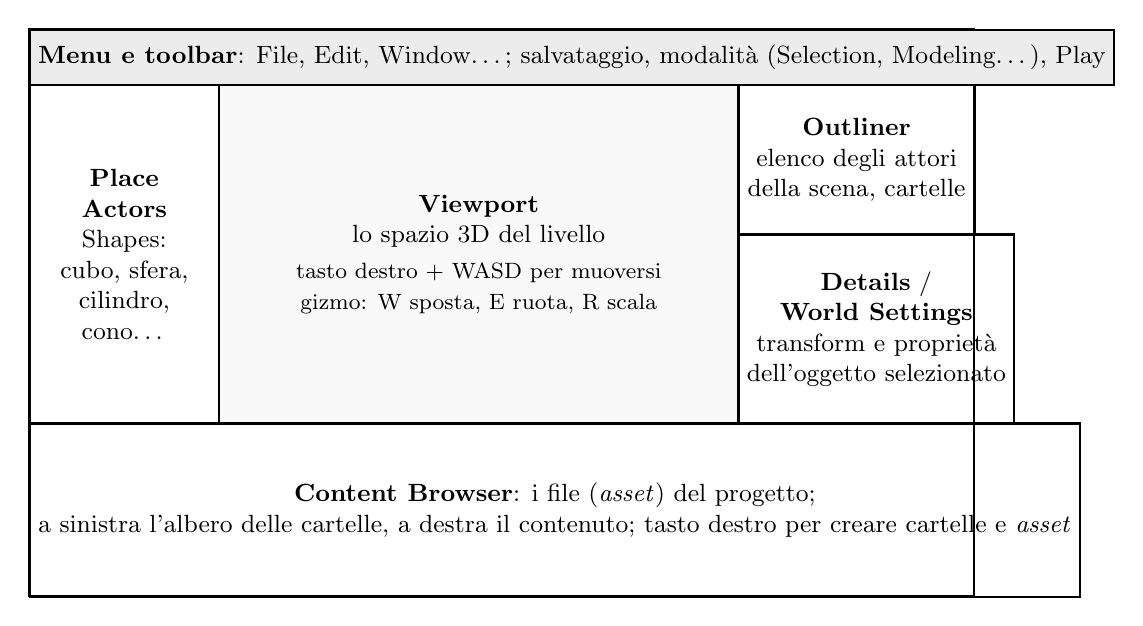
\begin{tikzpicture}[
  font=\small,
  ue1pan/.style={draw, thick, align=center, inner sep=3pt},
  ue1note/.style={font=\footnotesize, align=left, text width=3.4cm}
]
  % cornice
  \draw[thick] (0,0) rectangle (12,7.2);
  % toolbar
  \node[ue1pan, minimum width=12cm, minimum height=0.7cm, anchor=north west, fill=gray!15]
    at (0,7.2) {\textbf{Menu e toolbar}: File, Edit, Window\ldots; salvataggio, modalità
    (Selection, Modeling\ldots), Play};
  % place actors
  \node[ue1pan, minimum width=2.4cm, minimum height=4.3cm, anchor=north west]
    at (0,6.5) {\textbf{Place}\\\textbf{Actors}\\Shapes:\\cubo, sfera,\\cilindro,\\cono\ldots};
  % viewport
  \node[ue1pan, minimum width=6.6cm, minimum height=4.3cm, anchor=north west, fill=gray!5]
    at (2.4,6.5) {\textbf{Viewport}\\lo spazio 3D del livello\\[2pt]
    \footnotesize tasto destro + WASD per muoversi\\\footnotesize gizmo:
    W sposta, E ruota, R scala};
  % outliner
  \node[ue1pan, minimum width=3cm, minimum height=1.9cm, anchor=north west]
    at (9,6.5) {\textbf{Outliner}\\elenco degli attori\\della scena, cartelle};
  % details
  \node[ue1pan, minimum width=3cm, minimum height=2.4cm, anchor=north west]
    at (9,4.6) {\textbf{Details} /\\\textbf{World Settings}\\transform e proprietà\\
    dell'oggetto selezionato};
  % content browser
  \node[ue1pan, minimum width=12cm, minimum height=2.2cm, anchor=north west]
    at (0,2.2) {\textbf{Content Browser}: i file (\emph{asset}) del progetto;\\
    a sinistra l'albero delle cartelle, a destra il contenuto; tasto destro per creare
    cartelle e \emph{asset}};
\end{tikzpicture}
\caption{Una disposizione tipica dell'editor, come quella mostrata da Igor. Ogni pannello
si può spostare, agganciare ad altri o chiudere; il menu Window li riapre.}
\label{ue1:fig:editor}
\end{figure}

\paragraph{Le cartelle, e i loro colori.} Nel Content Browser, con il \textbf{tasto
destro}, si possono creare vari tipi di \emph{asset}; per cominciare, una cartella:
\textbf{New Folder}, chiamata ``prova''. Si possono creare tutte le cartelle che si
vogliono, ``in modo da avere ordine''. Una ``piccola chicchetta'': con il tasto destro
su una cartella, \textbf{Set Color}, la si può \textbf{colorare} (Igor la fa blu), un
feedback visivo che rende la navigazione molto più veloce. Il Content Browser mostra le
cartelle in due modi: a destra come in un \emph{explorer}, a sinistra come un albero ``a
cascata''. Se si mette una cartella dentro un'altra, a sinistra compare una piccola
freccia che apre la cartella sottostante: cartelle e sottocartelle.

\paragraph{L'ordine, per sé e per gli altri.} ``È molto importante l'organizzazione.'' Le
cartelle si riempiranno di \emph{asset}, e bisognerà cercarne uno solo senza sapere dove
andare. L'ordine serve ``non solo per la salvezza vostra, ma anche dei vostri possibili
collaboratori'': ``vi assicuro che quando siete ordinati, la gente vi ringrazia''.

\paragraph{Approfondimento: il Content Drawer e la definizione di \emph{asset}.} Nella
disposizione predefinita di Unreal Engine 5 il Content Browser non è sempre aperto: lo si
richiama dal pulsante \textbf{Content Drawer} in basso a sinistra (o con
Ctrl+Spazio), e lo si può agganciare stabilmente all'interfaccia (``Dock in Layout''),
come ha fatto Igor. Romero e Sewell definiscono l'\emph{asset} come ``un pezzo di
contenuto di un progetto Unreal'': materiali, \emph{static mesh} e Blueprint sono tutti
\emph{asset}. Quando si trascina un \emph{asset} dal Content Browser nel livello,
l'editor ne crea una \textbf{copia} da piazzare nella scena: l'\emph{asset} resta uno, le
sue istanze nel livello possono essere molte. Gli stessi autori descrivono l'Outliner
come l'elenco degli oggetti presenti nel livello, e i Details come il pannello che
mostra le proprietà modificabili dell'oggetto selezionato.

% ---------------------------------------------------------------------
\section{Il primo cubo e il \emph{transform}}
\label{ue1:sec:transform}

\paragraph{Place Actors.} Gli \emph{actor} sono gli elementi di gioco. Dal pannello
\textbf{Place Actors} (se manca: Window, Place Actors), nella sezione \textbf{Shapes},
si prende un \textbf{cubo} e lo si trascina nella viewport. ``Ecco a voi un cubetto
renderizzato'': il primo cubo in Unreal, ``e ne avrete tanti''.

\paragraph{I tre assi.} Sul cubo compaiono tre frecce: sono i tre assi principali,
\textbf{X}, \textbf{Y} e \textbf{Z}, lungo i quali lo si può muovere. Ogni asse ha il
suo colore: \textbf{X rosso}, \textbf{Y verde}, \textbf{Z blu}.

\paragraph{Il \emph{transform}.} Di ogni oggetto si possono modificare
\textbf{locazione}, \textbf{rotazione} e \textbf{scala}. L'insieme dei tre è il
\textbf{\emph{transform}} (``quando parleremo di \emph{transform}, ricordatevelo''), e
lo si rivedrà ``a oltranza''. Lo si modifica in due modi: con le frecce nella viewport,
o con i numeri nel pannello \textbf{Details}.

\paragraph{I numeri nei Details.} Nei Details la locazione del cubo è, per esempio, 480,
430, 120: è la \textbf{raffigurazione numerica}, in unità di Unreal, del punto in cui si
trova l'oggetto. Se si scrive 0 al posto del primo valore e si preme Invio, ``poplà'':
la coordinata X del cubo adesso è 0. Se si trascina una freccia guardando i numeri, si
vede il valore crescere o diminuire, andare in positivo o in negativo: è il verso
dell'asse.

\paragraph{Unreal ragiona in centimetri.} ``Molto importante'': \textbf{l'unità di Unreal
è il centimetro}. Se un oggetto va spostato di tre metri, lo si sposta di 300 unità.
Nella griglia del pavimento ogni riquadro, dice Igor, è un metro, e un cubo, di
default, è un metro.

\paragraph{W, E, R.} Il \textbf{pivot} (o \emph{gizmo}) è ``questo cosettino degli
assi'', e permette tre movimenti: con \textbf{W} si sposta (locazione), con \textbf{E} si
ruota, con \textbf{R} si scala. Gli stessi tre strumenti sono anche in alto a destra
nella viewport, come icone.

\paragraph{Assi locali e assi globali.} Esistono due riferimenti: gli assi
\textbf{relativi} all'oggetto stesso (\textbf{locali}) e quelli del \textbf{mondo}
(\textbf{globali}, la sua \emph{absolute location}). Finché il cubo non è ruotato la
differenza non si vede; ma se lo si ruota fino a farlo diventare ``una specie di rombo''
e si infila nel terreno, alzarlo lungo i suoi assi locali richiede ``un doppio
movimento, così e così'', perché gli assi locali ruotano insieme a lui (``avremo il
nostro bel pivot ruotato di 40 gradi''). Con gli assi globali, invece, l'alto è sempre
l'alto. Il passaggio dall'uno all'altro si fa con l'icona in alto nella viewport:
\textbf{il cubetto con tre assi} indica il riferimento \textbf{locale}, \textbf{il
mondo} indica quello \textbf{globale}. La scelta vale per locazione e rotazione.

\paragraph{La scala è solo locale.} Non vale per la scala: \textbf{un oggetto si può
scalare solo nei suoi assi locali}. Se si scalasse un oggetto ruotato lungo gli assi del
mondo, ``verrebbe totalmente stretchato malissimo'': l'oggetto è girato in un modo e
l'asse in un altro, e allungarlo così lo deformerebbe. Unreal ``ce lo impedisce''.

\paragraph{Le unità di misura del \emph{transform}.} La locazione è in centimetri, la
\textbf{rotazione in gradi} (``io l'ho ruotato e c'è un 40''), la \textbf{scala in
unità}: 1 è la dimensione originale, 2 il doppio.

\begin{figure}[htbp]
\centering
\begin{tikzpicture}[
  font=\small,
  ue1ax/.style={-{Stealth[length=3mm]}, very thick},
  ue1box/.style={draw, thick, rounded corners=3pt, text width=3.6cm, align=left,
               inner sep=5pt}
]
  % assi
  \coordinate (o) at (0,0);
  \draw[ue1ax, red!75!black] (o) -- (2.2,0) node[right]{X};
  \draw[ue1ax, green!50!black] (o) -- (1.2,1.1) node[above right]{Y};
  \draw[ue1ax, blue!75!black] (o) -- (0,2.2) node[above]{Z};
  \fill (o) circle (2pt);
  \node[below=0.2cm of o, font=\footnotesize, align=center]
    {pivot: X rosso, Y verde, Z blu};
  % riquadri
  \node[ue1box, right=2.8cm of o, yshift=1.6cm] (loc)
    {\textbf{Location} (\textbf{W})\\in centimetri\\locale o globale};
  \node[ue1box, below=0.25cm of loc] (rot)
    {\textbf{Rotation} (\textbf{E})\\in gradi\\locale o globale};
  \node[ue1box, below=0.25cm of rot] (sca)
    {\textbf{Scale} (\textbf{R})\\in unità (1 = originale)\\solo locale};
  \node[draw, thick, dashed, fit=(loc)(rot)(sca), inner sep=6pt,
    label={[font=\small\bfseries]above:Transform}] {};
\end{tikzpicture}
\caption{Gli assi e il \emph{transform}. Lo \emph{snapping} (sezione
\ref{ue1:sec:snap}) si imposta separatamente per ognuna delle tre componenti.}
\label{ue1:fig:transform}
\end{figure}

\paragraph{Il tasto Fine.} Un'altra ``piccola chicchetta'': se si piazza un cubo in
aria e si preme il tasto \textbf{Fine} (\emph{End}, quello ``sopra le frecce''), il cubo
cade sulla prima superficie che trova sotto di sé. ``Molto utile'', perché evita di
stare lì ad abbassarlo a occhio.

\paragraph{I Details seguono la selezione.} Ogni volta che si clicca un oggetto, i Details
mostrano \emph{quell'}oggetto: due cubi hanno due locazioni, due rotazioni, due scale.
\textbf{Per modificare i parametri di un oggetto, bisogna selezionarlo.}

\paragraph{Lavorare con i numeri.} I numeri dei Details sono lo strumento preciso, e
sono molto usati, per esempio, dai level designer: ``dobbiamo allargare il corridoio di
tre metri''. Igor allunga un cubo di tre metri sull'asse Y. Nei campi numerici si può
anche scrivere, oppure \textbf{trascinare}: si mette il mouse sul campo e lo si fa
scorrere a destra e a sinistra (``slidando'') per cambiare il valore, su qualunque asse,
per locazione, rotazione e scala.

\paragraph{Reset.} Accanto a ogni gruppo di valori c'è una \textbf{freccetta}: cliccandola,
il valore torna a quello originale (la scala torna a 1, la locazione al punto di
partenza).

% ---------------------------------------------------------------------
\section{Muoversi, duplicare, raggruppare}
\label{ue1:sec:navigazione}

\paragraph{Forme e pivot.} Si possono piazzare tanti \emph{actor} diversi: cilindri,
coni, sfere. Il pivot è al \textbf{centro} di ogni figura, e per questo un cilindro,
appena piazzato, è ``mezzo interrato''. Per \textbf{scalare su tutti gli assi
insieme} si prende il centro del gizmo di scala e si trascina verso l'esterno (allarga)
o verso l'interno (stringe); trascinando una sola maniglia si scala su un solo asse.

\paragraph{Duplicare con Alt.} Igor costruisce un tavolino con un cilindro schiacciato e
uno allungato. Serve un altro pezzo uguale: bisogna prendere un altro cilindro e rifare
tutto? No: \textbf{si tiene premuto Alt e si trascina} (o si ruota) l'oggetto, e se ne
crea una copia esatta. ``Lo userete a manetta.'' Funzionano anche \textbf{Ctrl+C} e
\textbf{Ctrl+V}. Una studentessa, abituata a Blender, si confonde: premeva Alt e lo
lasciava. Alt va \textbf{tenuto premuto mentre si trascina}, ``non è solo \emph{tap}
Alt''.

\paragraph{Muoversi nella viewport.} ``Mi sono dimenticato di dirvelo, perdonatemi'':
per muoversi nella viewport si tiene premuto il \textbf{tasto destro} del mouse e si
usano \textbf{W, A, S, D}, come in un gioco in prima persona; muovendo il mouse si
ruota la camera. Uno studente scopre da solo che \textbf{E} sale e \textbf{Q} scende:
``bravissimo, esatto''. Bisogna cliccare dentro la viewport: è la camera dell'editor,
non quella del gioco.

\paragraph{Seguire un oggetto.} Se si tiene premuto \textbf{Shift} mentre si trascina un
oggetto, la camera lo \textbf{segue} nel movimento: utile per piazzamenti
particolari.

\paragraph{Selezionare più oggetti.} Per selezionare più oggetti si tiene premuto
\textbf{Shift} (o Ctrl) e si cliccano uno dopo l'altro. Con il palo e il piano del
tavolo selezionati, Alt e trascinamento: ``pac!'', un secondo tavolino.

\paragraph{I gruppi.} Selezionare ogni volta tutti i pezzi è scomodo, perché se si
clicca il piano del tavolo si seleziona solo il piano. Si possono allora
\textbf{raggruppare}: si selezionano gli oggetti, tasto destro, \textbf{Group}, oppure
\textbf{Ctrl+G}. Intorno al gruppo compare ``una specie di reticolo verde'', e cliccando
un pezzo qualunque si seleziona il tutto. Si possono anche raggruppare dei gruppi, per
farne uno più grande. Per \textbf{sciogliere} un gruppo: \textbf{Shift+G}, oppure tasto
destro, Groups, \textbf{Ungroup}.

\paragraph{Ctrl+Z.} ``Qua funziona'': \textbf{Ctrl+Z} annulla. ``Sappiatelo, ogni
errore può essere cancellato, o almeno per poco.''

\paragraph{I gruppi non sono un oggetto unico.} Igor fa vedere un limite: se si
\textbf{scala} un gruppo, Unreal non lo scala come un oggetto unico; ogni pezzo si
scala rispettando i propri assi relativi. Per avere un oggetto davvero unico bisognerà
creare una \textbf{static mesh}, ``che vedremo in seguito''.

\paragraph{Mesh e static mesh.} Una \textbf{mesh} è un oggetto solido formato da
poligoni: quando qualcuno dice ``mi serve la mesh del tavolo'' intende il
\textbf{modello 3D} del tavolo. La \textbf{static mesh} è un tipo di mesh; esistono anche
le \textbf{dynamic mesh}, ``un discorso che vedremo più avanti''.

\paragraph{Approfondimento: \emph{transform} relativi nei Blueprint.} Il comportamento dei
gruppi anticipa un tema che nei Blueprint tornerà spesso. Romero e Sewell, nel capitolo
sui nodi matematici, distinguono il \textbf{\emph{transform} del mondo} di un attore
(la sua posizione assoluta nel livello) dal \textbf{\emph{transform} relativo} dei suoi
componenti, che è relativo al componente ``genitore''. Il loro esempio è un tavolo con
sopra una statua: se si sposta il tavolo, la statua lo segue; se si cambia il
\emph{transform} relativo della statua, il tavolo resta dov'è. È il modo in cui, dentro
una Blueprint Class, si costruiscono oggetti composti che si muovono come un tutt'uno.

% ---------------------------------------------------------------------
\section{Lo \emph{snapping} e la velocità della camera}
\label{ue1:sec:snap}

\paragraph{Lo \emph{snapping}.} Ruotando un oggetto, l'editor mostra un numero che sale
a scatti: 20, 30, 40, 50, 60, 70 gradi. È lo \textbf{\emph{snap}}, che si controlla in
alto a destra nella viewport: ci sono tre pulsanti, per locazione, rotazione e scala,
ognuno con un valore. \textbf{Se il pulsante è azzurro, lo \emph{snap} è attivo.}
\begin{itemize}
  \item Senza \emph{snap} di rotazione l'oggetto ruota liberamente, con i decimali; con
        lo \emph{snap} a 10, ruota di dieci gradi alla volta. Cliccando sul numero si
        sceglie il passo: 5, 10, 15, 30, 45, 60, 90, 120 gradi. Con 120, ``pam!'',
        diretto da 0 a 120; con 5, una rotazione più fine.
  \item Lo stesso vale per la \textbf{locazione}: con lo \emph{snap} l'oggetto si muove
        ``a scattini'' (di 1, 5, 10, 50 unità\ldots), senza si muove di qualunque
        valore, decimali compresi.
  \item E per la \textbf{scala}: senza \emph{snap} si scala ``quanto mi pare'', con lo
        \emph{snap} a passi anche molto piccoli, come 0,25.
\end{itemize}
Se lo \emph{snapping} impedisce di mettere un pezzo dove si vuole, ``basta
disattivarlo''.

\paragraph{La velocità della camera.} Per raggiungere ``quella montagna là'' si può
\textbf{velocizzare la camera}: mentre ci si muove (tasto destro premuto), si gira la
\textbf{rotellina del mouse} in avanti per andare più veloci e indietro per andare più
lenti, quando bisogna osservare un oggetto da vicino con precisione (Igor scende fino a
una velocità di 0,03 per guardare sotto il tavolino).

% ---------------------------------------------------------------------
\section{L'Outliner e l'ordine della scena}
\label{ue1:sec:outliner}

\paragraph{L'elenco della scena.} L'\textbf{Outliner} (se manca: Window, Outliner) è una
raffigurazione a lista di \textbf{tutti gli oggetti in scena}. Se si duplica un cono,
nell'Outliner compaiono Cone, Cone2, Cone3, Cone4\ldots{} Un oggetto si può selezionare
sia nella viewport sia nell'Outliner, ed è utile quando ``avete un bel \emph{pack} di
roba'' da gestire. Per eliminare un oggetto: \textbf{Canc} (\emph{Delete}).

\paragraph{Le cartelle dell'Outliner.} Anche nell'Outliner si possono creare cartelle, e
a Igor ``aiuta molto'' nella pianificazione e nel piazzamento. Tasto destro
nell'Outliner, \textbf{Create Folder}, e si crea una cartella ``Coni''. Poi si
selezionano i coni: visto che sono elencati per nome, si clicca il primo, si tiene
premuto \textbf{Shift} e si clicca l'ultimo, e si seleziona tutta la lista; si
trascinano dentro la cartella. Da quel momento, invece di cliccarli uno per uno, basta
il tasto destro sulla cartella e \textbf{Select All Descendants}: ``eccoli qua''.

\paragraph{Perché farlo subito.} ``Immaginatevi una scena intera, gigantesca.'' Senza
ordine si passano ``tre quarti d'ora'' a cliccare un oggetto dopo l'altro; con le
cartelle, un tasto e si è fatto. ``Vi risparmiate molto tempo.''

\paragraph{Il tasto G.} Un ultimo tasto, che Igor spiega durante la dimostrazione: se il
pivot ``scompare'', bisogna premere \textbf{G}. G passa dalla visualizzazione
dell'editor, con gli aiuti visivi, a quella ``normale'' del mondo di gioco, in cui gli
aiuti sono nascosti.

\paragraph{Approfondimento: la Game View.} Il comando si chiama \textbf{Game View}: con G
la viewport mostra la scena come la vedrebbe il giocatore, nascondendo icone,
\emph{gizmo} e oggetti che nel gioco sono invisibili (le icone delle luci, i volumi, i
punti di partenza del giocatore). È comodo per giudicare l'aspetto finale di una scena;
ma se lo si attiva per sbaglio sembra che gli strumenti siano spariti, ed è per questo
che Igor lo nomina proprio quando il pivot ``scompare''.

\begin{table}[htbp]
\centering
\small
\begin{tabular}{@{}p{4.3cm}p{8.7cm}@{}}
\toprule
\textbf{Comando} & \textbf{Che cosa fa} \\
\midrule
Tasto destro + W A S D & muoversi nella viewport; con il mouse si ruota la camera \\
Tasto destro + E / Q & salire / scendere \\
Rotellina (durante il movimento) & velocità della camera: avanti più veloce, indietro
  più lenta \\
W / E / R & gizmo di locazione / rotazione / scala \\
Icona cubetto / mondo & assi locali / globali (per locazione e rotazione) \\
Pulsanti azzurri dello \emph{snap} & attivano lo \emph{snapping} e ne scelgono il
  passo \\
Fine (\emph{End}) & fa cadere l'oggetto sulla superficie sottostante \\
Alt + trascinamento & duplica l'oggetto (Alt tenuto premuto) \\
Ctrl+C / Ctrl+V & copia e incolla \\
Shift + clic & selezione multipla; nell'Outliner, selezione di un intervallo \\
Shift + trascinamento & la camera segue l'oggetto \\
Ctrl+G / Shift+G & raggruppa / separa (anche: tasto destro, Groups) \\
Ctrl+Z & annulla \\
Canc (\emph{Delete}) & elimina l'oggetto selezionato \\
G & Game View: mostra o nasconde gli aiuti dell'editor \\
Freccetta accanto ai valori & riporta il valore all'originale \\
Ctrl+S & salva \\
\bottomrule
\end{tabular}
\caption{I comandi della prima lezione. Tutti valgono nel Level Editor di Unreal Engine
5.5 con le impostazioni predefinite.}
\label{ue1:tab:comandi}
\end{table}

% ---------------------------------------------------------------------
\section{Esercitazione: il ristorante dei tre tavoli}
\label{ue1:sec:esercitazione}

Con quello che si è imparato, ``una piccola esercitazione''. Bisogna costruire, con le
forme di base, \textbf{tre tavoli con le loro sedie}:
\begin{enumerate}
  \item un tavolo con \textbf{tre posti}: ``vengono tre ospiti a cena'';
  \item un \textbf{tavolo quadrato} per \textbf{cinque ospiti};
  \item una \textbf{cena romantica}: un tavolo per \textbf{due}, ``e se volete
        metteteci pure la candela''.
\end{enumerate}
Non serve una sedia precisa: ``l'importante è che applicate tutto quello che abbiamo
fatto''. Chi non riesce oggi può farlo per la volta successiva (``assolutamente''), e
riguardare la registrazione.

\paragraph{Partire da una reference.} Un consiglio, ``soprattutto per voi artisti'': per
fare qualcosa di artistico, prendere una \textbf{reference}. Ma non una sedia troppo
complessa: ``non ci interessa fare una cosa bella e bellissima''. Igor sceglie una
sedia ``molto semplice'', la ``sedia della nonna che vi fa il ragù''.

\paragraph{La dimostrazione.} Igor costruisce la sua sedia passo per passo, ed è un buon
riassunto di tutta la seconda parte:
\begin{enumerate}
  \item un cubo, scalato con lo \emph{snap} a 0,25, per la seduta; la freccetta di reset
        per riportarlo alle dimensioni di partenza quando serve (``le sedie sono alte
        più o meno un metro'');
  \item la prima gamba, posizionata (``se avete problemi con lo \emph{snapping}, basta
        disattivarlo'');
  \item le altre gambe: Shift per selezionare, Alt per duplicare. Ne viene ``questo
        bellissimo sgabello'', con le gambe ``non proprio precisissime'';
  \item lo schienale, duplicando altri pezzi per il dorso;
  \item tutti i pezzi selezionati e \textbf{Ctrl+G}, ``perché sennò dobbiamo fare ogni
        volta uno, due, tre, quattro'';
  \item la sedia accostata al tavolo (``è un po' spesso questo tavolo, ci saranno delle
        ginocchiate incredibili, ma non ci importa'').
\end{enumerate}

\paragraph{Si può allineare un oggetto a un altro?} Uno studente, che oggi può solo
guardare, chiede se c'è un modo di allineare le gambe della sedia a un oggetto, visto
che a mano non è semplice. Igor risponde che non è una cosa che in Unreal si fa
``professionalmente'': strumenti di allineamento precisi ci sono nei programmi di
modellazione, come Blender e Maya. In Unreal ci sono il tasto \textbf{Fine}, lo
\emph{snapping}, il lavoro ``un po' a mano'', i \emph{plugin}, oppure la
\textbf{Modeling Mode}, la modalità di modellazione dell'editor, con strumenti più
precisi, che si vedrà in seguito.

\paragraph{Gli strumenti si somigliano.} Lo stesso studente nota che, in attesa del
download, ha usato \textbf{Inkarnate}, un programma per disegnare mappe, e che i
principi visti finora sono ``molto simili''. ``Sì, assolutamente'': sono principi
condivisi dai vari game engine e dai programmi grafici. In Unity ``magari qualche
bottone è un po' diverso'', ma le funzioni sono simili; ``si impara a muoversi da una
parte e si impara a muoversi dall'altra''. Igor mostra anche \textbf{Dungeon
Scrawl}\footnote{Igor ci arriva per tentativi: ``Dungeon Crawler'', ``Dungeon
Designer'', ``Dungeon Scroll''.}, uno strumento per disegnare mappe per le partite di
D\&D con gli amici, usato anche per il level design.

\paragraph{I risultati.} Dopo una ventina di minuti di lavoro individuale, i
``ristoratori in erba'' mostrano i loro tavoli.
\begin{itemize}
  \item Uno studente ha aggiunto una \textbf{luce} per la candela, ma la candela fa
        ombra. Igor gli mostra come risolvere: si seleziona la luce e nei Details, in
        basso, si toglie la spunta a \textbf{Cast Shadows}.
  \item Qualcuno ha fatto un tavolo rettangolare invece che quadrato: ``va benissimo,
        tranquilli''.
  \item Uno studente, che ha appena finito il download, ha fatto solo la base del tavolo
        e una gamba della sedia, sottilissima. Igor ricorda che Unreal lavora in
        centimetri, e quella gamba è di pochi centimetri: ``non ci farei sedere
        nessuno, potrebbe crollare''. Ma ``è soggettivo''.
\end{itemize}
``A parte l'ironia'', la conclusione è che gli oggetti in sé contano poco: conta capire
come ci si muove in Unreal, duplicando, scalando, muovendo, ruotando. ``Questa è la cosa
più importante che oggi impariamo.''

\paragraph{Una cartella per ogni tavolo.} Un'ultima richiesta: mettere ogni gruppo in una
cartella dell'Outliner. Create Folder, ``Tavolo da due'', si selezionano i pezzi e li si
trascina dentro; poi ``Tavolo da tre'', e così via. Con Select All Descendants si
riprende il tavolo intero in un clic.

% ---------------------------------------------------------------------
\section{Salvare la mappa, e la chiusura}
\label{ue1:sec:chiusura}

\paragraph{Salvare.} Per salvare il lavoro c'è il classico \textbf{Ctrl+S}. Siccome la
mappa è stata creata ``da nulla'', la prima volta Unreal chiede dove salvarla: le si dà
un nome (``MappaProva'') e la si salva dentro la cartella ``prova'' del Content
Browser. In basso a destra, poi, l'editor tiene il conto delle modifiche non salvate:
se si sposta anche solo una sedia, compare l'indicazione degli oggetti
\textbf{\emph{unsaved}}, ``tutti gli oggetti che devo salvare''.

\paragraph{Che cos'è il secondo file?} Uno studente nota che il salvataggio crea anche un
secondo file, un \textbf{HLOD Layer}\footnote{Nella trascrizione ``Halodle'' e ``Halod
Layer''.}. Igor spiega che dipende dalla mappa: quella su cui hanno lavorato contiene un
\textbf{landscape}, le montagne che si vedono in fondo. Il landscape è un piano che si
può modellare con uno strumento apposito per formare, per esempio, il paesaggio di
sfondo; il file salva come quel piano è composto. La volta successiva si userà una
mappa davvero vuota, senza landscape.

\paragraph{Approfondimento: LOD e HLOD.} \textbf{LOD} sta per \emph{level of detail}:
lo stesso oggetto esiste in più versioni, con un numero decrescente di poligoni, e
l'engine usa quelle più semplici quando l'oggetto è lontano dalla camera, dove i
dettagli non si vedrebbero comunque. È la risposta pratica al compromesso della
sezione~\ref{ue1:sec:rendering} tra precisione e peso. Gli \textbf{HLOD}
(\emph{hierarchical} LOD) fanno lo stesso a livello di gruppi: interi blocchi lontani
della mappa vengono sostituiti da un'unica versione semplificata. Le mappe ``a mondo
aperto'' di Unreal Engine 5, con il landscape, li usano per impostazione predefinita, ed
è per questo che il salvataggio crea un file di \emph{HLOD Layer}.

\paragraph{Le ultime domande.} Come si separano gli oggetti raggruppati? ``Shift+G, oppure
tasto destro, Ungroup: se lo cerchi c'è proprio scritto.'' Quando arriva la
registrazione? Sul sito, ``credo il giorno dopo''. Le foto dei lavori si possono mandare
a Igor su Discord, ``tranquillamente'' (``quando ci sono, vi rispondo''), anzi in un
\emph{thread} o un canale apposito, ``così almeno è più ordinato e non mi riempite la
casella privata''.

\paragraph{Il calendario.} Giovedì si rivede Igor; il martedì successivo c'è Davide, con
la parte artistica; poi le lezioni si alternano, ``settimana a settimana''. Sono le 19:
``per chi tra poco cena, auguro buona cena a tutti''. ``Se avete domande, fatele adesso o
tacete fino alla prossima volta.'' ``Ciao, ragazzi.''

% ---------------------------------------------------------------------
\section*{Punti chiave del capitolo}
\addcontentsline{toc}{section}{Punti chiave del capitolo}

\begin{itemize}
  \item Il \textbf{game engine} è ``il calderone'' che riunisce 3D art, programmazione e
        design in un unico ambiente, con fisica e collisioni, suono, animazione,
        networking e IA. Lo si governa con lo \textbf{scripting}; in Unreal, con i
        \textbf{Blueprint}, un linguaggio a nodi usato anche dai programmatori (il C++
        resta per ottimizzare). Conta la \textbf{logica}, più dello strumento.
  \item Il \textbf{rendering} trasforma poligoni in pixel: \textbf{\emph{vertex
        shading}} (i vertici dei triangoli), \textbf{rasterizzazione} (quali pixel),
        \textbf{\emph{fragment shading}} (colore, luce, ombre, riflessi). Più poligoni
        = più precisione, ma più peso: ``un cubo con due milioni di poligoni'' fa
        esplodere il gioco.
  \item Il \textbf{\emph{real time rendering}} lavora tra 20 e 120 \emph{fps}: il cinema
        è a 24, il gaming a 30--60 e oltre. Un \textbf{frame} è un'immagine; la loro
        successione dà l'illusione del movimento.
  \item Unreal è il più usato perché è un \textbf{linguaggio comune}, aggiornato di
        continuo, e perché permette di \textbf{prototipare} subito: ``non ci interessa
        se è bello o brutto, è importante che funzioni'' (il prototipo di
        \emph{Expedition 33}). È usato anche nel cinema, dove conta il dettaglio più
        dell'ottimizzazione.
  \item Ciò che distingue un videogioco da un video è il \textbf{game loop}: input,
        \emph{update}, render, e di nuovo, a ogni \emph{frame}.
  \item \textbf{Ogni buona idea non esiste finché non sta su carta.} Indie, AA e AAA si
        distinguono per i soldi e per la specializzazione dei ruoli (fino ai \emph{leaf
        artist}). L'\textbf{\emph{outsourcing}} è chiedere a un altro studio una parte
        del lavoro, senza cedergli la proprietà.
  \item Tutti i ruoli toccano l'engine: \emph{blockout} e metriche per il level
        designer, momenti scriptati per il narrative designer, parametri esposti per il
        combat designer, materiali e Sequencer per gli artisti, rendering, IA e rete per
        i programmatori, Unreal Insights per il QA. \textbf{Trattate bene i vostri
        programmatori.}
  \item Un gioco è fatto di \textbf{attori, meccaniche, spazio, obiettivi, regole} (e a
        volte \textbf{tempo}); il divertimento è una \textbf{conseguenza}, e il gameplay
        nasce dalle \textbf{scelte}. Meccanica = che cosa posso fare; dinamica = come lo
        faccio; estetica = come mi fa sentire. ``Un gioco per tutti non è un gioco per
        nessuno.''
  \item Il bilanciamento è un lavoro tra \textbf{designer e QA}; il feedback utile è
        quello da cui si ricava un'informazione. Far giocare chi non ha mai visto il
        gioco ``è la cosa più pura''.
  \item Per il corso serve Unreal \textbf{5.5} (la 5.5.4): l'ultimo numero è solo
        l'aggiornamento, il secondo decide la compatibilità.
  \item Le risorse: \textbf{documentazione}, forum, corsi gratuiti di
        \emph{learning}, \textbf{Fab} con i \emph{pack} gratuiti del mese (``prendeteli
        sempre''). Ma \textbf{prima la funzione, poi l'\emph{asset}}, o il progetto
        pesa 70~GB per usarne tre.
  \item Quando si preme Play gli attori vengono inizializzati e duplicati. Ogni
        movimento va reso \textbf{relativo al tempo di gioco} (\emph{delta seconds}),
        altrimenti dipende dagli \emph{fps}.
  \item Il progetto di prova: Games, \textbf{Blank}, Blueprint, Desktop, Starter
        Content, nome \textbf{senza spazi}. I template si distinguono per le
        \textbf{3C}: camera, controller, character.
  \item L'editor è fatto di \textbf{finestre} spostabili (Window le riapre): viewport,
        Details, Outliner, World Settings, \textbf{Content Browser}. Cartelle colorate
        e ordine: ``quando siete ordinati, la gente vi ringrazia''.
  \item Il \textbf{transform} è locazione (\textbf{centimetri}), rotazione
        (\textbf{gradi}) e scala (\textbf{unità}); \textbf{W, E, R}; X rosso, Y verde,
        Z blu; assi locali o globali, ma \textbf{la scala è solo locale}.
  \item \textbf{Alt + trascinamento} duplica, \textbf{Ctrl+G} raggruppa, \textbf{Fine}
        appoggia a terra, lo \textbf{\emph{snap}} azzurro fa muovere a scatti, la
        \textbf{rotellina} cambia la velocità della camera, \textbf{Select All
        Descendants} riprende un'intera cartella dell'Outliner.
\end{itemize}

%
%  Tutte le etichette di questo capitolo hanno il prefisso "ue1:"
%  (ue1:cap:..., ue1:sec:..., ue1:fig:..., ue1:tab:...), e tutti gli
%  stili TikZ hanno il prefisso "ue1" (ue1box, ue1arr, ...) per non
%  collidere con chiavi native di TikZ. Il capitolo è autonomo: non
%  contiene \ref verso altri capitoli.
%  Le figure sono ricostruzioni schematiche di quanto mostrato e detto a
%  lezione, non copie delle slide del docente. Dove la trascrizione è
%  troppo rovinata per ricostruire un dettaglio, il capitolo lo dice
%  invece di inventarlo.
% =====================================================================

\chapter[Introduzione a Unreal Engine]{Introduzione a Unreal Engine: che cos'è un
engine, chi lo usa, e il primo contatto con l'editor}
\label{ue1:cap:intro}

Questa è la \textbf{prima lezione} del corso breve di \textbf{introduzione a Unreal
Engine}, un corso che ha il suo centro nei \textbf{Blueprint}, il sistema di
programmazione visuale ``a nodi'' dell'engine di Epic Games. La lezione ha due metà
molto diverse. La prima è teorica e larga: che cos'è un \emph{software}, che cos'è un
\emph{game engine}, come un modello fatto di poligoni diventa un'immagine sullo
schermo, perché Unreal è oggi l'engine più diffuso, quali figure di una produzione lo
usano e per che cosa, e infine, con un'attività in classe, da che cosa è formato un
gioco. La seconda metà è pratica: si scarica Unreal Engine 5.5, si guardano le risorse
che Epic mette a disposizione (la documentazione, i corsi gratuiti, il negozio di
\emph{asset} Fab), si crea un primo progetto vuoto e si impara a muoversi nell'editor:
piazzare un cubo, spostarlo, ruotarlo, scalarlo, duplicarlo, raggrupparlo, ordinarlo
in cartelle. La lezione si chiude con un'esercitazione: arredare un piccolo
ristorante con tre tavoli e le loro sedie.

Il docente è \textbf{Igor}\footnote{Il docente si presenta come ``Igor Ripanti''; il
cognome è quello della trascrizione automatica, che altrove storpia quasi tutti i nomi
propri, e il capitolo non è in grado di verificarlo.}, che si presenta come ex alunno
della stessa scuola degli studenti, ``precisamente per quanto riguarda game
design''\footnote{La trascrizione dice ``sono stato un alunno di Live'': il nome della
scuola è con ogni probabilità storpiato.}. Ha lavorato a \textbf{\emph{Steel Seed}},
``principalmente come \emph{level designer}''; ma ``essendo un ambiente indie'' faceva
``un po' di tutto'', anche programmazione e \emph{scripting}, e quindi ha fatto ``uso
intensivo'' di Unreal Engine ``e di tutte le sue feature''. Il corso è diviso tra due
docenti: con Igor la parte di programmazione e di ``piccole feature''; con
\textbf{Davide}, a partire dal 26 del mese, una parte ``un po' più artistica''. Le
lezioni si alternano: il giovedì successivo gli studenti saranno di nuovo con Igor, il
martedì dopo con Davide.

La lezione è \textbf{online}, su Zoom, con un server Discord del corso per i
materiali e le domande; inizia poco dopo le 17 e finisce alle 19, con una pausa di una
decina di minuti verso le 17 e mezza\footnote{Igor, credendo per errore che la lezione
finisse alle 18 (``sono da un altro corso che finiva alle 18''), dopo la pausa annuncia
che ``manca mezz'ora alla fine''; gli studenti lo correggono (``nella mail c'era
scritto'' alle 19), e il docente ha ``un'altra ora'' per la parte pratica.}. Gli
studenti sono tutti \textbf{nuovi iscritti al primo anno}, di corsi diversi: game
design (la maggioranza), narrative design, character animation, 3D art e
programmazione. Il corso breve, in altre parole, è comune a figure che in una
produzione useranno Unreal in modi molto diversi, ed è proprio da questa varietà che
Igor parte.

Tre avvertenze di lettura. La prima: la trascrizione è automatica e storpia moltissimi
nomi. Unreal diventa ``Arreal'', ``Arial Engine'', ``ArrayLange'', ``ArrayLab'',
``Arrival Engine'', ``Arrial'', ``Ariane Engine'', ``Riala'' e ``a Real Engine'';
\emph{Clair Obscur: Expedition 33} è ``Expedition'' e ``Spedisce 33''; Sandfall
Interactive è ``Send Follow Interactive''; \emph{shader} è anche ``scender''. Dove la
ricostruzione è sicura il capitolo usa la forma corretta e, la prima volta, lo segnala
in nota; dove non lo è riporta la forma della trascrizione e lo dice. La seconda: in
più punti la registrazione contiene lunghi blocchi di testo senza senso e ripetuto
(``qual è la risposta che ci può essere?'', ``a parte il plus time\ldots''): sono
artefatti del riconoscimento vocale durante la pausa e i momenti di lavoro
individuale, e il capitolo li ignora. La terza: la seconda metà della lezione è una
dimostrazione dal vivo nell'editor; il capitolo ricostruisce i passaggi da ciò che Igor
dice mentre li fa, e li completa, dove serve, con i nomi esatti dei comandi.

\paragraph{Come leggere questo capitolo.} Il capitolo segue l'ordine della lezione.
Le figure ricostruiscono gli schemi spiegati a voce o sulle slide (la pipeline di
rendering, il \emph{game loop}, gli elementi di un gioco, l'interfaccia dell'editor,
il \emph{transform}); le tabelle riassumono i ruoli della produzione e le scorciatoie
da tastiera della seconda parte. Qua e là, dei paragrafi di \textbf{approfondimento}
collegano la lezione al libro \emph{Blueprints Visual Scripting for Unreal Engine 5}
di Marcos Romero e Brenden Sewell, che sarà il testo di riferimento per questa parte
del libro, e a qualche nozione tecnica generale; sono segnalati come tali e non fanno
parte della lezione.

Il percorso del capitolo:
\begin{enumerate}
  \item le presentazioni e le esperienze degli studenti (sezione
        \ref{ue1:sec:presentazioni});
  \item il \textbf{software}, il \textbf{game engine} e lo \textbf{scripting}, con i
        Blueprint (sezione \ref{ue1:sec:engine});
  \item il \textbf{rendering 3D}: poligoni, \emph{vertex shading}, rasterizzazione,
        \emph{fragment shading}; poi il \emph{real time rendering} e i \emph{frame}
        (sezioni \ref{ue1:sec:rendering} e~\ref{ue1:sec:realtime});
  \item \textbf{Unreal Engine}: perché è così usato, la prototipazione, i giochi, gli
        engine di una volta, il cinema, il \textbf{game loop} (sezioni
        da~\ref{ue1:sec:unreal} a~\ref{ue1:sec:gameloop});
  \item la \textbf{produzione} e i \textbf{ruoli} che toccano l'engine (sezioni
        \ref{ue1:sec:produzione} e~\ref{ue1:sec:ruoli});
  \item l'attività in classe: \textbf{da che cosa è formato un gioco}, e le domande
        prima della pausa (sezioni \ref{ue1:sec:elementi} e~\ref{ue1:sec:domande});
  \item il \textbf{download} della 5.5, le \textbf{risorse} (documentazione,
        \emph{learning}, Fab) e un po' di teoria sul \emph{Play in Editor} e sul
        \emph{delta time} (sezioni da~\ref{ue1:sec:download} a~\ref{ue1:sec:pie});
  \item il primo contatto con l'\textbf{editor}: il progetto, l'interfaccia, il
        \textbf{transform}, la navigazione, l'organizzazione (sezioni
        da~\ref{ue1:sec:progetto} a~\ref{ue1:sec:outliner});
  \item l'\textbf{esercitazione dei tre tavoli}, il salvataggio e la chiusura (sezioni
        \ref{ue1:sec:esercitazione} e~\ref{ue1:sec:chiusura}).
\end{enumerate}

% ---------------------------------------------------------------------
\section{Presentazioni: chi c'è, e chi ha già aperto un engine}
\label{ue1:sec:presentazioni}

La lezione comincia con qualche minuto di attesa (``aspettiamo cinque, dieci minuti''),
un appello e una richiesta: accendere la webcam, ``così almeno ci vediamo un po' in
faccia''. A chi non ha una webcam Igor suggerisce le applicazioni che trasformano il
telefono in una webcam, ``come se ti facessi una videochiamata'': lui usa di solito
\emph{Iriun}\footnote{Nella trascrizione ``Ingur'' e ``Iruin''; si tratta con ogni
probabilità di \emph{Iriun Webcam}, un'applicazione gratuita che fa esattamente
questo.}. I lavori in corso nell'edificio del docente producono ``rumori molesti'' per
tutta la lezione, e Igor se ne scusa.

Poi il giro di presentazioni: nome, corso, ``un piccolo background''. Tutti sono iscritti
al primo anno; i corsi sono game design, character animation, narrative design (più di
uno), 3D art e programmazione. ``C'è una bella quantità di nuovi compagni di design'',
commenta Igor, ``quindi avremo pane per i nostri denti'', oltre ovviamente a 3D art e
programmazione.

\paragraph{Chi ha già usato un engine?} La domanda successiva è se qualcuno abbia ``mai
aperto un software di \emph{develop} per i videogiochi'': Unity, Godot, ``in
generale''. Qualcuno ha provato Godot; qualcuno un po' di Unity, seguendo un corso
online ``molto veloce'' e facendo ``un paio di giochini'', un \emph{platform} e un clone
di \emph{Flappy Bird}, ``di 3D niente''; qualcuno è ``digiuno'', e qualcun altro ha
lavorato ``con roba presa da Fab''. Igor accoglie tutte le risposte allo stesso modo:
``ci sta assolutamente''. Fab, aggiunge, sarà uno dei temi di oggi, perché è ``una
risorsa incredibile'', soprattutto per le cose gratis, quelle in sconto e i contenuti
gratuiti del mese.

\paragraph{La mentalità prima degli strumenti.} A chi parte da zero Igor dà subito una
rassicurazione che vale per tutto il corso: ``l'importante è avere la mentalità''. In
programmazione, ``molto spesso'' si tratta ``semplicemente'' di imparare a usare gli
strumenti, mentre ``la logica fa da padrone''. Passare da un engine all'altro, o da
nessun engine al primo, è soprattutto ``riabituarsi a un nuovo campo di gioco''.

% ---------------------------------------------------------------------
\section{Software, game engine e scripting}
\label{ue1:sec:engine}

\paragraph{Che cos'è un software.} Igor parte dalla definizione più semplice possibile:
il \textbf{software} è ``quello che non è hardware, fondamentalmente''. È un insieme di
istruzioni, di dati e di programmi con funzionalità precise, che ci permettono di
creare cose: strumenti di 3D art come \textbf{Blender} e \textbf{Maya}, oppure
\emph{engine} come \textbf{Unreal Engine} e \textbf{Unity}.

\paragraph{L'engine come calderone.} Il \textbf{game engine} è ``il calderone, chiamiamolo
un po' così'', che riunisce tutte le facoltà di chi sviluppa (3D art, programmazione,
design) e le mette ``in un ambiente comune'', l'ambiente di sviluppo dell'engine. Gli
engine più noti sono \textbf{Unreal}, \textbf{Unity}, \textbf{Godot} e
\textbf{GameMaker}, e ognuno contiene al suo interno molte funzionalità: i
\textbf{motori fisici}, che gestiscono le \textbf{collisioni}; la gestione dei
\textbf{suoni}; le \textbf{animazioni}; il \textbf{networking}; l'\textbf{intelligenza
artificiale} dei personaggi. Nessuna di queste cose ``si fa da sola'': ci mettono le
mani gli sviluppatori, ``tramite lo \emph{scripting}''.

\paragraph{Lo scripting, e i Blueprint.} Lo \textbf{scripting} è ``la forma di
programmazione che ci permette di entrare in interazione e creare cose all'interno
dell'engine''. Esistono molti linguaggi: Igor cita il \textbf{C}, il \textbf{C\#}
(quello di Unity) e i \textbf{Blueprint}, che sono il tipo di \emph{scripting} di Unreal
Engine e l'oggetto di questo corso. Più avanti nella lezione (sezione~\ref{ue1:sec:ruoli})
Igor tornerà sul punto: in Unreal si può programmare anche in codice (in C++), ``ma noi
non lo useremo'', perché i Blueprint bastano ``tranquillamente'', sono usati anche dai
programmatori, e ``tanti giochi nel comparto indie'' sono fatti ``solo con Blueprint,
senza mai toccare una riga di codice''. I Blueprint sono un \textbf{linguaggio a nodi}:
``prendiamo proprio e colleghiamo tutti i nodini'' per dare un senso alla
programmazione.

\paragraph{Approfondimento: le due accezioni di ``Blueprint''.} Romero e Sewell, nel
primo capitolo di \emph{Blueprints Visual Scripting for Unreal Engine 5}, fanno notare
che in Unreal la parola \emph{Blueprint} ha due significati. È il nome del
\textbf{linguaggio di scripting visuale} creato da Epic Games; ed è anche il nome di un
\textbf{tipo di oggetto di gioco} creato con quel linguaggio. I Blueprint di questo
secondo tipo sono di due specie: il \textbf{Level Blueprint}, uno per ogni livello del
gioco (non se ne possono creare altri separati), e le \textbf{Blueprint Class}, che
servono a creare oggetti interattivi riutilizzabili in qualunque livello. Un progetto di
Unreal Engine 5, aggiungono gli autori, si può sviluppare in Blueprint, in C++ o in una
combinazione dei due: si può aggiungere codice C++ a un progetto Blueprint e viceversa.
La scelta di partire dai Blueprint, quindi, non chiude nessuna porta.

% ---------------------------------------------------------------------
\section{Il rendering 3D: dai poligoni ai pixel}
\label{ue1:sec:rendering}

Un'applicazione grafica come un gioco 3D ha una particolarità: il \textbf{3D
rendering}, cioè ``la fase finale dello sviluppo di un'immagine''. È il processo che
prende un \textbf{\emph{3D asset}} (``per il linguaggio un po' più tecnico'') e ci
presenta davanti la scena vera e propria, con gli oggetti creati dai 3D artist ``che
hanno faticato tanto per poterlo fare''. Quegli oggetti sono formati da
\textbf{poligoni}.

\paragraph{Quanti poligoni ha questo oggetto?} Igor chiede se qualcuno ha mai sentito
parlare del numero di poligoni di un modello. Uno studente sì: gli sono capitati ``dei
video di ottimizzazione'' su come diminuire i poligoni ``per cercare di diminuire il
\emph{lag}''. ``Esatto, bravissimo.'' La regola è semplice, e Igor la dice con una
battuta: ``se mai doveste avere il caso fortuito di avere un cubo con due milioni di
poligoni, sappiate che il vostro gioco esploderà, probabilmente''. Nella
\textbf{viewport} (``un elemento che poi vedremo'': la finestra in cui l'engine, ma
anche Blender mentre si modella, mostra la scena) vale sempre lo stesso compromesso:
\textbf{più poligoni ci sono, più l'immagine è precisa, ma più è pesante da
renderizzare}.

\paragraph{Le tre fasi.} Il rendering di un'immagine passa per molti passaggi; ``noi oggi''
ne guardiamo tre principali (figura~\ref{ue1:fig:pipeline}).
\begin{enumerate}
  \item \textbf{\emph{Vertex shading}.} Le immagini e i modelli sono formati
        principalmente da \textbf{triangoli}, e i triangoli sono formati da
        \textbf{vertici}. I vertici definiscono la forma: in questa fase si
        identificano e si posizionano i tre punti di ogni triangolo.
  \item \textbf{Rasterizzazione.} Il triangolo così definito viene
        \emph{rasterizzato}: si stabilisce quali \textbf{pixel} dello schermo cadono
        dentro quel triangolino. Igor la spiega a partire dalla grafica 2D (``qualcuno
        ha fatto grafica?'', e una studentessa laureata in grafica conferma). Un'immagine
        \textbf{raster}, come quelle di Photoshop, è fatta di pixel; un'immagine
        \textbf{vettoriale} è fatta di vettori. La differenza: se si ingrandisce
        (``strecciate'') un'immagine raster, diventa ``sgranatissima''; un'immagine
        vettoriale la si può ingrandire ``quanto volete'' e resta uguale. Gli schermi,
        però, sono fatti di pixel: per questo i triangoli vanno rasterizzati.
  \item \textbf{\emph{Fragment shading}.} È la fase finale, quella ``vicina alla
        visualizzazione''. Ai \textbf{frammenti} (``poligoni, triangoli, chiamateli
        come vi pare'') si applicano i \textbf{colori}, la \textbf{luce}, le
        \textbf{ombreggiature} e i \textbf{riflessi}, tenendo conto della posizione
        della camera. È anche ``una parte molto artistica'', perché Unreal lavora molto
        sulla resa della luce: si possono piazzare luci, gestire come la luce entra in
        una stanza, e così via.
\end{enumerate}

\begin{figure}[htbp]
\centering
\begin{tikzpicture}[
  font=\small,
  ue1box/.style={draw, thick, rounded corners=3pt, minimum height=1.5cm,
               text width=2.6cm, align=center},
  ue1io/.style={draw, thick, dashed, rounded corners=3pt, fill=gray!10,
               minimum height=1.5cm, text width=2.0cm, align=center},
  ue1arr/.style={-{Stealth[length=3mm]}, thick}
]
  \node[ue1io] (m) {\textbf{Modello 3D}\\poligoni\\(triangoli)};
  \node[ue1box, right=0.5cm of m] (v) {\textbf{1. Vertex shading}\\i vertici
    definiscono la forma dei triangoli};
  \node[ue1box, right=0.5cm of v] (r) {\textbf{2. Rasterizzazione}\\quali pixel
    cadono dentro ogni triangolo};
  \node[ue1box, right=0.5cm of r] (f) {\textbf{3. Fragment shading}\\colore, luce,
    ombre, riflessi};
  \node[ue1io, below=0.8cm of f] (s) {\textbf{Immagine}\\sullo schermo\\(pixel)};
  \draw[ue1arr] (m) -- (v);
  \draw[ue1arr] (v) -- (r);
  \draw[ue1arr] (r) -- (f);
  \draw[ue1arr] (f) -- (s);
  \node[below=0.9cm of v, text width=6.2cm, align=left, font=\footnotesize] {Più
    poligoni $\Rightarrow$ immagine più precisa, ma più pesante da renderizzare
    (``un cubo con due milioni di poligoni'' fa esplodere il gioco).};
\end{tikzpicture}
\caption{Le tre fasi principali del rendering di cui parla Igor. Il processo reale ha
molti passaggi intermedi; la lezione si ferma a questi tre.}
\label{ue1:fig:pipeline}
\end{figure}

\paragraph{Per vertici o per frammenti.} Sulla slide, in basso a destra, ci sono due
versioni della stessa sfera illuminata. Nella prima la luce è calcolata \textbf{per
vertici}: la luce ``quasi'' lascia vedere i triangoli. Nella seconda è calcolata
\textbf{per frammenti}, cioè dopo il \emph{fragment shading}: la luce è ``molto più
diramata'', morbida, ``e fa sì che funzioni per bene''.

\paragraph{Le UV.} Igor accenna anche alle \textbf{UV}, di cui si parlerà più avanti nel
corso: sono ``delle mappe che i 3D artist creano'' e che permettono di dire come il
materiale si comporta sulla superficie del modello, come gestire e rifrangere la luce,
``questo materiale così'', e così via.

\paragraph{Approfondimento: che cosa sono le UV.} Per completezza (la lezione ci torna
solo di sfuggita): le \textbf{coordinate UV} sono il modo in cui la superficie di un
modello 3D viene ``srotolata'' su un piano a due dimensioni, come si apre la scatola di
cartone di un cubo. Le lettere U e V indicano i due assi di quel piano, per non
confonderli con gli X, Y e Z dello spazio 3D. Su quel piano si dipingono le
\emph{texture} (il colore, la rugosità, i dettagli in rilievo), che poi l'engine
``riavvolge'' sul modello durante il rendering. Un buon \emph{UV mapping} è il motivo
per cui una texture appare senza deformazioni o cuciture visibili.

% ---------------------------------------------------------------------
\section{Il \emph{real time rendering} e i \emph{frame}}
\label{ue1:sec:realtime}

In Unreal Engine il rendering è \textbf{in tempo reale}. Igor lo collega a un'esperienza
che molti studenti faranno: lo \emph{showreel}, soprattutto per chi diventerà 3D artist,
sarà ``molto accompagnato'' dal rendering di Unreal, con camere ed effetti ``fatti per
bene, scriptati'', che permettono di vedere gli oggetti ``alla massima qualità
possibile''. E come sempre: più alta è la qualità, più tempo ci vuole per renderizzare.
Il \emph{real time rendering} è il rendering che produce le immagini a una velocità
compresa, più o meno, tra i \textbf{20 e i 120 fotogrammi al secondo}.

\paragraph{Che cos'è un frame.} Un \textbf{frame} (fotogramma) è una singola immagine; la
\textbf{visualizzazione per frame} è un susseguirsi di immagini correlate l'una
all'altra che danno l'\textbf{illusione del movimento} sullo schermo. È lo stesso
principio dell'animazione: il cinema lavora a \textbf{24 \emph{frame} al secondo}
(``quando andate a vedere un film''), il gaming di solito a \textbf{30 o 60
\emph{fps}}, e c'è chi gioca a 120--144 \emph{fps} (``incredibili'', commenta Igor,
``l'\emph{fps} che se la tira tanto'').

\paragraph{Approfondimento: il budget di un frame.} Un modo utile per leggere questi
numeri è rovesciarli. A 30 \emph{fps} l'engine ha circa $1000/30 \approx 33$
millisecondi per produrre ogni immagine; a 60 \emph{fps} ne ha circa 16,7; a 120 circa
8,3. In quel tempo deve leggere gli input, aggiornare la logica di gioco (il
\emph{game loop} della sezione~\ref{ue1:sec:gameloop}) e renderizzare la scena. È per
questo che l'ottimizzazione (meno poligoni, meno luci dinamiche, nebbia più leggera)
non è un dettaglio tecnico ma una condizione per avere un gioco giocabile: tutto ciò che
non entra nel \emph{budget} fa scendere il \emph{frame rate}.

% ---------------------------------------------------------------------
\section{Unreal Engine: perché è così usato}
\label{ue1:sec:unreal}

Unreal Engine è ``il nostro bellissimo'' game engine, quello che si userà per tutto il
corso. È sviluppato da \textbf{Epic Games}, e per usarlo bisogna scaricare
l'\textbf{Epic Games Launcher} dal sito di Epic (lo si farà durante la lezione, sezione
\ref{ue1:sec:download}).

\paragraph{Il più usato.} È, dice Igor, ``proprio il più usato al momento'': ``gran parte
dei giochi moderni'', AA e AAA, tendono a usarlo. Una delle ragioni è che, essendo un
motore comune, Epic lo aggiorna continuamente, con nuove funzionalità come il
\textbf{Control Rig}, che permette per esempio di fare le animazioni in modo
procedurale. Nel launcher si vede: ogni volta propone una versione diversa da scaricare
(5.5, 5.6, 5.7\ldots), e il canale YouTube ufficiale di Unreal Engine pubblica a ogni
versione un video riassuntivo delle novità.

\paragraph{Un linguaggio comune.} La seconda ragione è che Unreal è un \textbf{linguaggio
comune}: permette ai professionisti di parlarsi e di produrre insieme. I designer, per
esempio, lo usano ``molto spesso per prototipare''. La \textbf{prototipazione} è una
fase ``molto importante'' della creazione di un gioco: ``tiro fuori l'idea dal
cappello'' e la si mette ``direttamente in engine'', usando lo \emph{scripting} per
vedere se ``questa idea che ho in testa funziona''. È ``il modo più veloce e più giusto
per capire subito se qualcosa funziona''. Poi ci sono molte altre figure che usano
l'engine nelle sue diverse caratteristiche (sezione~\ref{ue1:sec:ruoli}).

\paragraph{Alcuni giochi fatti in Unreal.} Sulla slide: \emph{A Way Out}, \emph{Ark},
\emph{Crash Bandicoot 4} (``per chi ha giocato, bellissimo'') e \emph{Fortnite}. Per
\emph{Fortnite} esiste anche una versione dell'engine, \textbf{Unreal Editor for
Fortnite} (UEFN), che permette di prendere le funzionalità del gioco e ``metterle
insieme''. Igor lo paragona a \textbf{Roblox}, che sta facendo ``un simile effetto'':
creare un \textbf{mega \emph{game template}}. Un \emph{game template} è ``il
\emph{pattern} di regole'', tutto ciò che forma il gioco, messo a disposizione delle
persone perché ci facciano ``quello che vogliono''.

\paragraph{Il caso \emph{Expedition 33}.} Igor chiede quale gioco fatto in Unreal sia
rimasto in testa agli studenti, e la risposta arriva subito: \textbf{\emph{Clair
Obscur: Expedition 33}}\footnote{Nella trascrizione quasi sempre solo ``Expedition'' o
``Expedition 33'', una volta ``Spedisce 33''.}. ``Benissimo, vedo che ci intendiamo.''
Il gioco, racconta Igor, è nato da persone che, ``per quanto dicano loro'', hanno
detto: ``non sapevamo fare un gioco, e ci siamo messi a guardare YouTube''. Igor mostra
il video del \textbf{prototipo} di \emph{Expedition 33} fatto in Unreal Engine (dopo la
solita pubblicità): è lo stadio che si affronta ``molto spesso all'inizio di una
produzione'', quello in cui ``non ci interessa se è bello o brutto, è importante che
funzioni''. Unreal permette proprio questo: mettere subito in campo le cose più usate
del gaming.

\paragraph{Le cose comuni.} Ci sono infatti tante cose ``comuni all'interno del nostro
panorama videoludico''. Il \textbf{salto}, per esempio: ``quante volte in un gioco si
salta?''. C'è chi non lo usa, ma i giochi con il salto sono ``a bizzeffe''. Unreal,
creando una sorta di \emph{template} comune, facilita molto i primi passi.

% ---------------------------------------------------------------------
\section{Gli engine di una volta, e Unreal fuori dai videogiochi}
\label{ue1:sec:storia}

\paragraph{Quando ogni gioco aveva il suo engine.} ``Non siamo lì, ragazzi, nel 2004.'' Nei
vecchi giochi, ricorda Igor, si creavano engine \textbf{apposta}: un programmatore
doveva passare dalle linee di codice alla visualizzazione in 3D, ``in tutto un processo
che andava dai due ai tre anni''. E quegli engine erano poco riutilizzabili, perché
contenevano ``\emph{pattern} di regole molto fissati''. Si trovavano comunque modi
interessanti di riusarli: Igor cita, come ``piccola curiosità'', un gioco di Shrek per
PlayStation~2 (``Shrek~2'', si corregge) realizzato modificando il motore di un gioco
del \emph{Signore degli Anelli}\footnote{L'aneddoto è riportato come lo racconta Igor,
che lo introduce con ``io mi ricordo''; il capitolo non ha verificato quale gioco del
\emph{Signore degli Anelli} e quale versione di \emph{Shrek} siano coinvolti.}.

\paragraph{Gli engine proprietari.} Esistono poi gli engine \textbf{proprietari}, come
\textbf{Source} e \textbf{Source~2} di Valve (\emph{Half-Life}): sono ``loro'', di Valve,
ma la casa mette a disposizione gratuitamente gli strumenti per creare mappe, con
l'editor \textbf{Hammer}. Unreal, invece, mette a disposizione ``tante cose diverse''
per ``mettere subito la carne sul fuoco'' e facilitare il progetto.

\paragraph{Unreal nel cinema.} Oltre ai videogiochi, Unreal è ``molto usato'' nel
\textbf{\emph{filmmaking}} e nel \emph{videomaking}. Igor mostra uno spot di
motociclette (``della Indian''): le rocce intorno al motociclista ``non esistono'', sono
renderizzate in Unreal. È ``la classica storia del \emph{green screen}'', con dietro il
lavoro di chi è esperto di Unreal. Uno studente ricorda che anche \emph{The Batman} fu
girato in parte in questo modo, e Igor conferma che ``se ne parlò'': oggi è ``molto in
voga'', perché ``nessuno ha voglia di andare di nuovo in Islanda'' per avere delle
rocce molto belle; ci si fa le rocce pre-renderizzate.

\paragraph{Ottimizzazione contro dettaglio.} I processi, però, sono ``molto
differenziati''. Nei videogiochi si parla molto di \textbf{ottimizzazione}: modelli
\textbf{\emph{low poly}}, non pesantissimi e non precisissimi, ``belli da vedere ma
ottimizzati''. Nel \emph{filmmaking} l'ottimizzazione esiste, ma conta il
\textbf{dettaglio}, perché il risultato è ``solo una raffigurazione''. Un videogioco,
invece, è \textbf{un programma in esecuzione}: continui \emph{frame}, continue
interazioni, un continuo \emph{game loop}.

\paragraph{Le rocce che si vedono ovunque.} Una battuta tra sviluppatori: esistono rocce
che ``sono le stesse, perché sono bellissime''. Sono fatte in 4K e
\textbf{scannerizzate}: qualcuno si è messo letteralmente a fotografare le rocce, le ha
digitalizzate e le ha messe gratis sull'\emph{asset store}. ``E le vedete ovunque'':
``ormai sono riconoscibili'', fatte molto bene ma molto comuni.

\paragraph{Approfondimento: \emph{virtual production} e \emph{scan}.} Le due cose di cui
parla Igor hanno un nome. La prima è la \textbf{\emph{virtual production}}: invece di
aggiungere lo sfondo in post-produzione su un \emph{green screen}, si proietta in
tempo reale l'ambiente renderizzato da Unreal su grandi pareti di LED intorno agli
attori, così che luci e riflessi siano già giusti in ripresa (la tecnica è stata resa
celebre da \emph{The Mandalorian}). La seconda è la \textbf{fotogrammetria}: si
fotografa un oggetto reale da decine o centinaia di angolazioni e un software ne
ricostruisce il modello 3D con le texture. Le rocce ``che si vedono ovunque'' vengono
quasi certamente dalla libreria \textbf{Quixel Megascans}, che Epic ha acquisito e reso
gratuita per Unreal, e che oggi è distribuita attraverso Fab.

% ---------------------------------------------------------------------
\section{Il \emph{game loop}}
\label{ue1:sec:gameloop}

Che cosa succede, allora, ``all'interno di un \emph{frame}'' di un gioco? Il
\textbf{\emph{game loop}} (figura~\ref{ue1:fig:gameloop}) è il ciclo che distingue un
videogioco da un video:
\begin{enumerate}
  \item si \textbf{inizializza} il gioco;
  \item il programma è \textbf{in attesa di un input} e lo legge: ``io premo X, A, o
        quello che è'';
  \item dopo l'input c'è un \textbf{\emph{update}}: a livello di programmazione il
        personaggio salta, si ha il movimento;
  \item si \textbf{renderizza} l'immagine;
  \item se si esce dal gioco il processo finisce; altrimenti si ricomincia dal punto 2,
        ``in questo iter continuo''.
\end{enumerate}
La differenza sostanziale tra il \emph{videomaking} e ``un vero videogioco'' è proprio
la presenza del \emph{game loop}.

\begin{figure}[htbp]
\centering
\begin{tikzpicture}[
  font=\small,
  ue1box/.style={draw, thick, rounded corners=3pt, minimum height=1.1cm,
               text width=2.6cm, align=center},
  ue1end/.style={draw, thick, rounded corners=8pt, fill=gray!15,
               minimum height=0.9cm, text width=2.0cm, align=center},
  ue1dec/.style={draw, thick, diamond, aspect=2, inner sep=1pt, text width=1.6cm,
               align=center},
  ue1arr/.style={-{Stealth[length=3mm]}, thick}
]
  \node[ue1end] (init) {Inizializzazione};
  \node[ue1box, right=0.9cm of init] (in) {\textbf{Input}\\attesa e lettura\\(premo A)};
  \node[ue1box, right=0.9cm of in] (up) {\textbf{Update}\\logica di gioco\\(il personaggio salta)};
  \node[ue1box, below=1.1cm of up] (re) {\textbf{Render}\\si disegna\\il frame};
  \node[ue1dec, left=1.1cm of re] (q) {Si esce dal gioco?};
  \node[ue1end, left=0.9cm of q] (fine) {Fine};
  \draw[ue1arr] (init) -- (in);
  \draw[ue1arr] (in) -- (up);
  \draw[ue1arr] (up) -- (re);
  \draw[ue1arr] (re) -- (q);
  \draw[ue1arr] (q) -- node[above, font=\footnotesize]{sì} (fine);
  \draw[ue1arr] (q) -- node[right, font=\footnotesize]{no: frame successivo} (in);
\end{tikzpicture}
\caption{Il \emph{game loop} come lo descrive Igor. Ogni giro del ciclo produce un
\emph{frame}: a 60 \emph{fps}, sessanta giri al secondo.}
\label{ue1:fig:gameloop}
\end{figure}

\paragraph{Approfondimento: l'evento Tick.} Nei Blueprint il \emph{game loop} si vede in
modo molto concreto. L'evento \textbf{Event Tick} viene eseguito \textbf{una volta per
ogni \emph{frame}}, e porta con sé un valore, \textbf{Delta Seconds}, che è il tempo
trascorso dal \emph{frame} precedente. È il punto in cui, nei Blueprint, si mette la
logica che deve aggiornarsi di continuo (un oggetto che ruota, una barra che si
riempie); ed è anche il motivo per cui Igor, più avanti nella lezione (sezione
\ref{ue1:sec:pie}), insiste sul rendere i movimenti ``relativi al tempo di gioco''.

% ---------------------------------------------------------------------
\section{La produzione: idee su carta, indie, AA, AAA}
\label{ue1:sec:produzione}

Una produzione ha molte figure (``ognuno di voi è programmazione, 3D artist, game
design''), e tutte si incontrano in un punto comune: Unreal Engine. Prima dello
sviluppo, però, c'è la \textbf{pre-produzione}, in cui si gestisce l'idea.

\paragraph{Lo storyboard.} Igor chiede chi sappia che cos'è uno \textbf{storyboard}: una
studentessa che ha studiato cinema e televisione, e una che ha lavorato in animazione,
ne hanno ``un minimo di base''. In pre-produzione bisogna capire che cosa si vuole fare,
perché se arriva qualcuno a dire ``io ho l'idea del secolo'', la risposta è: ``sì, ma
me la devi far capire''. \textbf{Ogni buona idea non esiste finché non sta su carta} e
non viene compresa da tante altre persone.

\paragraph{La documentazione.} Per i designer, la carta è la \textbf{documentazione}:
``noi designer facciamo documenti'', spieghiamo le meccaniche ``anche nel minimo
dettaglio'', soprattutto per le figure più in alto nella gerarchia.

\paragraph{Indie, AA, AAA.} La differenza tra le produzioni \textbf{indie},
\textbf{AA} (``doppia A'') e \textbf{AAA} (``tripla A'') è soprattutto una differenza
di soldi: quelli che i giochi producono (lo suggerisce uno studente) e soprattutto
quelli ``che ci si mette dietro'', e quindi le possibilità.
\begin{itemize}
  \item Nell'\textbf{indie} si lavora in team piccoli: ``al massimo'' venti persone,
        venti--trenta, e ``trenta già siamo abbastanza''. Le figure sono poco
        separate: ``mi puoi fare la programmazione, ma io sono un designer, e vabbè'',
        è stata ``molto la mia esperienza''.
  \item Il \textbf{AA} è ``una media impresa'': ci sono soldi, ma non come nel AAA, e
        le figure ``aleggiano'' spesso tra l'indie e l'AA, perché ``quando c'è
        necessità si fa virtù''. Anche \emph{Expedition 33} è un AA, ``che comunque
        c'ha tanti soldi''.
  \item Nel \textbf{AAA}, più si sale, \textbf{più preciso è il ruolo}. ``Ci sono
        artisti che fanno solo foglie'': i \emph{leaf artist}, che studiano ``tutte le
        particolarità di una foglia'', come cade, come il vento agisce su di essa, le
        sue nervature, come si differenzia nell'ambiente, come è ottimizzata.
\end{itemize}

\paragraph{L'\emph{outsourcing}.} Sandfall Interactive\footnote{Nella trascrizione
``Send Follow Interactive''.}, lo studio di \emph{Expedition 33}, ha usato
l'\textbf{\emph{outsourcing}} per le animazioni: secondo Igor sono state fatte in
Corea. Uno studente definisce l'\emph{outsourcing}, correttamente: è ``affidare alcune
parti della produzione ad altri studi''; ``esatto, bravissimo''. Un altro studente cita
il remake di \emph{Warcraft~III}, fatto da uno studio esterno, ``se non sbaglio
coreano''. Igor accetta l'esempio, ma aggiunge una precisazione importante: quando c'è
la \emph{ownership} del prodotto, cioè quando lo studio esterno ha la proprietà di ciò
che fa, ``quello non è \emph{outsourcing}''. L'\emph{outsourcing} è quando ``io sono
l'azienda X, vado dall'azienda Y e le chiedo: senti, mi puoi fare le animazioni? Mi
puoi fare il \emph{level design}?''.

% ---------------------------------------------------------------------
\section{Chi usa l'engine, e per che cosa}
\label{ue1:sec:ruoli}

I ruoli si distinguono per anzianità (``il classico'' \textbf{junior}, \textbf{mid} e
\textbf{senior}) e per area. Sulla slide le aree sono sei: \textbf{produzione},
\textbf{audio}, \textbf{programmazione}, \textbf{design}, \textbf{visual art} e
\textbf{business} (``\emph{miscellaneous}'': ci finiscono anche, per esempio, i
recensori e le testate giornalistiche come IGN). Per ognuna Igor racconta come si
interfaccia con Unreal (tabella~\ref{ue1:tab:ruoli}).

\paragraph{Design.} Tre esempi.
\begin{itemize}
  \item Il \textbf{game designer}, per esempio un \emph{combat designer}, crea
        \textbf{situazioni prototipate} di combattimento usando dei \emph{pattern}
        creati in Unreal dal programmatore. Lavora su richiesta: ``mi serve che questo
        parametro sia esposto, così lo posso muovere''. Quanto danno fa, per esempio.
  \item Il \textbf{level designer} lavora con il \textbf{\emph{blockout}} (o
        \emph{grey box}, \emph{white box}). ``Il \emph{blockout} è la forma primordiale
        di un livello'': non serve che il livello sia ``fatto, finito e compiuto,
        tutto bello, bellissimo'', ma che le forme riportino la loro
        \textbf{funzionalità}, che poi il 3D artist renderà belle. Nel \emph{blockout}
        si definiscono gli spazi e le \textbf{metriche}: quanta distanza c'è, se è
        abbastanza per sparare, se si vede bene il nemico. Lo si fa in Unreal, anche con
        il \textbf{Modeling Tool} (la modalità di modellazione dell'editor), meno
        preciso di Blender ma comodo per fare forme ``un po' più carine''. Sulla slide,
        un \emph{blockout} di \emph{Uncharted} di Emilia Schatz: ``queste sono le prime
        immagini che i level designer danno agli artisti''.
  \item Il \textbf{narrative designer} inserisce dialoghi e \textbf{momenti
        scriptati}: il personaggio che parla tra sé, il punto in cui si può giocare,
        quello in cui il personaggio discute, l'NPC con cui si interagisce. Il
        programmatore, ``molto spesso in relazione con il narrative designer'', crea
        sistemi prototipati e porta tutto a finalizzazione; se si è un
        \emph{technical} (narrative designer), lo si fa in parte da sé. Le figure di
        design sono molto collegate, perché ``i livelli devono avere un contesto'':
        ``ambientato in una fabbrica'' e ``una fattoria'' sono livelli totalmente
        diversi.
\end{itemize}

\paragraph{Visual art.} Qui l'engine entra in molti modi.
\begin{itemize}
  \item I \textbf{materiali}: nelle \emph{texture} si può ``mettere delle logiche'' e
        farle muovere. La lava che scorre ``molto spesso è un'immagine ferma'' che si
        muove grazie ai materiali di Unreal; o si usano effetti di
        \textbf{tassellazione} che fanno ``molleggiare'' la superficie.
  \item L'\textbf{animazione}, con il \textbf{Sequencer}: permette di fare animazioni in
        tempo reale dentro il gioco, momenti scriptati come una \emph{cutscene}
        ``in live'', scatole che cadono, un'astronave che passa davanti. Igor mostra un
        video di \emph{Star Wars Jedi: Fallen Order}: oltre alle \emph{cutscene}
        principali ci sono eventi ``totalmente scriptati'', come una piccola navicella
        che passa mentre il personaggio parla, o le navicelle tutto intorno.
        Sono animazioni ``in modo cinematografico'', fatte molto spesso con il
        Sequencer, e spesso volute dal narrative design.
  \item Il \textbf{concept art} non ha un uso molto particolare dentro l'engine, ma
        può servire, soprattutto se si parla di 2D, perché anche in Unreal si possono
        fare giochi 2D.
  \item Il \textbf{VFX artist}, che lavora con i sistemi di particelle (Niagara, di cui
        si parlerà più avanti).
  \item Il \textbf{technical artist}, la figura che sta tra programmazione e parte
        artistica e ``riesce a mettere in relazione le due cose''.
  \item L'\textbf{animatore}, di cui si è già detto.
\end{itemize}

\paragraph{Programmazione.} ``Io già do un consiglio ai designer: \textbf{trattate bene i
vostri programmatori}, sempre.'' La finalizzazione di tutte le idee che vengono in testa
ai designer ``è loro''. Anche qui, più si sale nell'industria, più i ruoli sono
sezionati:
\begin{itemize}
  \item il \textbf{combat programmer} e il \textbf{3C programmer}, dove le
        \textbf{3C} sono \emph{camera}, \emph{controller} e \emph{character};
  \item il \textbf{rendering engineer} (o \emph{engine programmer}), che lavora su come
        l'immagine viene renderizzata. Unreal è un engine a \textbf{sorgente aperto}:
        lo si può aprire e dire ``ti cambio la visualizzazione di come renderizzi una
        certa cosa''. L'esempio è il remake di \emph{Silent Hill~2}: la
        \textbf{nebbia} è ``la parte più importante'', e ``pesa tantissimo''; per
        avere un gioco pieno di nebbia senza che vada ``a scatti'' serve un rendering
        della nebbia ottimale, ed è il lavoro di questa figura;
  \item l'\textbf{AI programmer};
  \item chi si occupa del \textbf{networking}, per il multiplayer (client e server, ``un
        po' complesse'');
  \item e figure più esterne, per database e servizi.
\end{itemize}
Il linguaggio di codice di Unreal è il C++\footnote{Nella lezione Igor dice ``C'';
il linguaggio di Unreal Engine è il C++.}, ``ma noi non lo useremo'': per Unreal basta il
\textbf{Blueprint}, che ``è usato dai programmatori'' (``quindi, programmatori, non
scappate''). Il C++ si usa per esempio per ottimizzare certi processi, ``però
l'interfaccia principale è sempre Blueprint''. E ``tanti giochi nel comparto indie''
sono fatti solo con i Blueprint.

\paragraph{Audio.} Nessuno studente è del corso di audio, ma l'audio è gestito da Unreal
anche a livello di programmazione: si possono \textbf{randomizzare} i suoni, o
\textbf{modularli}, con un modulatore presente nell'engine.

\paragraph{Produzione.} Il \emph{playtesting}, la segnalazione dei \emph{bug}, la
gestione del progetto. Il \emph{producer} lavora soprattutto su altre piattaforme; il
\textbf{game tester} usa di più l'engine, per esempio con \textbf{Unreal Insights}, uno
strumento che risponde a domande come ``quante cose sono visualizzate a schermo qua
sopra, e quanto è pesante?''.

\paragraph{Business.} La parte ``più esterna'' usa l'engine poco, ma lo usa: per
l'\textbf{eseguibile}, e per le \textbf{\emph{build} di \emph{debug}} che vengono
presentate, per esempio, ai giornalisti. Sono \emph{build} con la facoltà di ``mettere i
\emph{cheat}'', per saltare parti del gioco o andare direttamente a una certa mappa,
``come i codici di una volta'' (``non sono così anziano, però\ldots'').

\begin{table}[htbp]
\centering
\small
\begin{tabular}{@{}p{2.3cm}p{4.2cm}p{6.6cm}@{}}
\toprule
\textbf{Area} & \textbf{Figure citate} & \textbf{Come usano Unreal} \\
\midrule
Design & game (combat) designer, level designer, narrative designer &
  prototipi di combattimento con parametri esposti; \emph{blockout} e metriche dei
  livelli, Modeling Tool; dialoghi e momenti scriptati \\
Visual art & materiali, animatori, concept artist, VFX artist, technical artist, leaf
  artist & materiali con logica (lava, tassellazione); Sequencer per eventi
  scriptati; 2D; particelle; ponte tra arte e codice \\
Programmazione & combat e 3C programmer, rendering/engine programmer, AI programmer,
  network & Blueprint (e C++ per ottimizzare); modifica del rendering (la nebbia di
  \emph{Silent Hill~2}); IA; client e server \\
Audio & sound designer & randomizzazione e modulazione dei suoni \\
Produzione & producer, game tester (QA) & \emph{playtesting}, \emph{bug},
  gestione; Unreal Insights per misurare il peso della scena \\
Business & stampa, marketing & eseguibile; \emph{build} di \emph{debug} con
  \emph{cheat} per i giornalisti \\
\bottomrule
\end{tabular}
\caption{Le aree di una produzione e il loro rapporto con l'engine, come le presenta
Igor. Dentro ogni area i ruoli si distinguono anche per anzianità: junior, mid,
senior.}
\label{ue1:tab:ruoli}
\end{table}

% ---------------------------------------------------------------------
\section{Attività in classe: da che cosa è formato un gioco?}
\label{ue1:sec:elementi}

La pausa, propone Igor, si può fare subito o più tardi; la classe preferisce ``verso le
5'', e si va avanti ancora un quarto d'ora con un'attività: ``per voi, da che cosa è
formato un gioco? Quali sono gli elementi che formano un gioco?''.

\paragraph{Prima risposta, e una correzione di rotta.} La prima risposta è da
\emph{game designer}: l'idea, il prototipo su cui si basa la struttura, le meccaniche
di gameplay, la parte artistica, il concept art, il sonoro. Igor la accoglie (``ok, ok,
ok''), ma la riorienta: non i componenti di una produzione, ma gli elementi di un gioco
qualunque. ``Facciamo acchiapparello'' (o ``ce l'hai'', come lo chiama qualcuno):
perché si chiama gioco? ``Proprio una parola, ragazzi.''

\paragraph{Le risposte della classe.} Arrivano una per volta.
\begin{itemize}
  \item Le \textbf{regole}: ``è formato da una serie di regole''. ``Bravo, regole.''
        Quindi una struttura.
  \item Il \textbf{divertimento}. Igor lo ridimensiona: il divertimento è ``una
        conseguenza''.
  \item L'\textbf{interazione}, un modo di interagire col gioco; e, detto ``in un
        altro modo, un po' filosofico'', i \textbf{giocatori}: ``se non c'è nessuno
        che gioca\ldots''. ``Bravissimo!'' I giocatori sono gli
        \textbf{attori}: è il termine che si ritroverà in Unreal (gli
        \emph{actor}), dove gli attori sono ``gli oggetti di gioco''. Altri li chiamano
        \emph{game object}, ``ognuno li chiama a modo suo''. Ci sono anche gli
        elementi sociali: la \textbf{socialità} ``è comunque gameplay'', nei giochi da
        festa come negli MMO (\emph{World of Warcraft}), che si basano ``tantissimo''
        sulla componente sociale.
  \item Dalla chat: \emph{Homo Ludens} (``bello'', commenta Igor), e l'osservazione che
        la definizione è complessa, perché ``molti giochi fanno anche a meno'' di
        certe componenti\footnote{Lo studente cita un esempio che la trascrizione rende
        con ``Three Monkeys''; Igor ammette di non conoscerlo.}. ``Giustissimo'': sono
        definizioni su cui anche nel panorama dello sviluppo ``c'è sempre un'opinione
        un po' diversa''.
  \item Un \textbf{obiettivo}: ``bravissimo''. È il movente, ``perché giochiamo, alla
        fine'', ed è una cosa ``molto psicologica''.
  \item Le \textbf{meccaniche}, cioè i modi di fare: ``io sparo o salto''. Con le
        meccaniche definiamo la tipologia di gioco: \emph{souls-like},
        \emph{roguelike} sono ``macro termini'' che raffigurano che cosa si può fare in
        un gioco, e anche le sue regole.
  \item Lo \textbf{spazio}. Igor lo cerca con una domanda (``quello che abbiamo intorno
        a noi''; ``l'ambiente di gioco?''; ``in che senso?''), finché arriva la
        parola: lo spazio, il \textbf{\emph{game space}}. Acchiapparello in un
        parchetto o in spiaggia non è lo stesso gioco; nel calcio ``c'è il fuorigioco
        perché c'è lo spazio che lo definisce''. Lo spazio di gioco è la mappa, il
        corridoio che si percorre.
  \item Il \textbf{tempo}, ``volendo'': anche il tempo può essere una regola (``devi
        fare questa cosa entro un tot, devi scappare'').
\end{itemize}

\begin{figure}[htbp]
\centering
\begin{tikzpicture}[
  font=\small,
  ue1core/.style={draw, thick, circle, minimum size=2.2cm, align=center,
               fill=gray!10},
  ue1elem/.style={draw, thick, rounded corners=3pt, minimum height=1cm,
               text width=2.7cm, align=center},
  ue1arr/.style={-{Stealth[length=2.5mm]}, thick}
]
  \node[ue1core] (g) {\textbf{Gioco}};
  \node[ue1elem, above left=0.5cm and 1.3cm of g] (att) {\textbf{Attori}\\giocatori,
    \emph{game object}};
  \node[ue1elem, above right=0.5cm and 1.3cm of g] (mec) {\textbf{Meccaniche}\\che cosa
    posso fare};
  \node[ue1elem, left=1.3cm of g] (reg) {\textbf{Regole}\\la struttura};
  \node[ue1elem, right=1.3cm of g] (spa) {\textbf{Spazio}\\il \emph{game space}};
  \node[ue1elem, below left=0.5cm and 1.3cm of g] (obi) {\textbf{Obiettivi}\\perché
    gioco};
  \node[ue1elem, below right=0.5cm and 1.3cm of g] (tem) {\textbf{Tempo}\\(a volte)
    una regola};
  \foreach \n in {att,mec,reg,spa,obi,tem} \draw[ue1arr] (\n) -- (g);
  \node[below=1.6cm of g, text width=10cm, align=center, font=\footnotesize]
    {Il \textbf{divertimento} non è un elemento ma una \emph{conseguenza}; le
     \textbf{scelte} che questi elementi permettono creano il gameplay.};
\end{tikzpicture}
\caption{Gli elementi di un gioco emersi dall'attività in classe. Il termine
``attori'' anticipa gli \emph{actor} di Unreal.}
\label{ue1:fig:elementi}
\end{figure}

\paragraph{L'\emph{escape room}.} Igor ha lavorato in una \emph{escape room} (``ragazzi,
io ci ho lavorato''), e la propone come caso: anche l'\emph{escape room} è un gioco,
perché ha tutti questi elementi. ``Definitemi attori, meccaniche, spazi, obiettivi e
regole; uno per volta, se no ci sovrapponiamo.'' Risponde una studentessa che ha
esperienza da \emph{game master}:
\begin{itemize}
  \item bisogna intanto \textbf{stabilire i confini}, ``una cosa molto importante'':
        ``molto spesso le persone arrivano senza regole e distruggono cose, rovinano la
        scenografia''. Igor lo chiama il \textbf{\emph{behavior}}: ``non fare la persona
        brutta'';
  \item bisogna stabilire una \textbf{chimica di gruppo} e dei \textbf{ruoli}: c'è
        sempre quello ``più scafato'', che cerca in giro ed è veloce, e quello che ci
        mette tanto ``ma poi arriva alla fine dell'enigma''. I ruoli fanno la forza del
        gruppo, perché ognuno sa che cosa deve fare;
  \item bisogna \textbf{non perdere tempo}, concentrarsi sulle cose giuste, ``ma senza
        farsi prendere dall'ansia'', ``perché è pur sempre un gioco''.
\end{itemize}

\paragraph{La scelta crea il gameplay.} Igor sottolinea l'ultimo punto: ``bisogna gestire
l'ansia, bisogna capire che cosa è importante''. Il gioco ``sta anche lì'', nella
\textbf{capacità di scelta} del giocatore. Ad acchiapparello si può giocare
nascondendosi e aspettando che qualcuno arrivi per fargli ``lo sgambettino'', oppure
inseguendo tutti ``a prescindere'', facendo ``un \emph{randomizer}'', andando ``a
cavolo''. Questo insieme di cose crea scelta, e quindi crea \textbf{gameplay}. Il
gameplay è spesso personalizzabile negli spazi che lo sviluppatore concede.

\paragraph{Lo spazio oltre lo schermo.} Lo spazio di gioco è lo schermo, la mappa; ma lo
si può anche allungare, rompendo la quarta parete. Gli \textbf{ARG}
(\emph{alternate reality game}\footnote{Nella trascrizione ``Artero Diperiale di
Game''.}) sono giochi che escono dal gioco: per aprire una porta bisogna andare a
cercare la risposta su un sito internet. È uno spazio di gioco che ``si è esternato''.

\paragraph{\emph{Expedition 33}: perché si gioca?} Poi un videogioco. Igor propone
\emph{Expedition 33} (``ve la butto lì''; ``eh vabbè, non vale, è il mio preferito''),
abbastanza fresco per tutti, insieme a un secondo titolo scelto da una
studentessa\footnote{La trascrizione lo rende con ``Barbarschettere'' e ``Barbara
Street~3'': potrebbe trattarsi di \emph{Baldur's Gate~3}, ma la ricostruzione non è
sicura.}. La domanda è: \emph{perché} si gioca? La studentessa risponde per
\emph{Expedition 33}: l'ha iniziato dopo i trailer, colpita dalla qualità della
\emph{motion capture} (``alcune volte mi sembra di vedere un film''), e perché ha ``un
debole per i giochi strazianti'' (``quando ho capito che avrei sofferto, ho detto: ecco
il gioco per me''). Ma è rimasta stupita dal combattimento: ha giocato tantissimo a
\emph{Final Fantasy~X}, che ama per la storia, ma non è un'amante dei giochi a turni, e
trova invecchiato il combattimento a turni di quel \emph{Final Fantasy}.
\emph{Expedition 33} l'ha trovato ``molto fresco'': ha rinnovato una cosa ``invecchiata
male'', con un gameplay ``che non è perfetto'' ma che ha portato a un gioco a turni
anche chi li odiava. In sintesi: si gioca per la bellezza del gameplay, la ricchezza
dell'arte e la trama.

\paragraph{Un gioco per tutti non è un gioco per nessuno.} Igor generalizza: ognuno porta
nel gioco ``una sua ricerca personale'', dentro il proprio ``spettro psicologico''. Sulla
slide c'è una frase attribuita ad Arrowhead Game Studios con cui Igor è ``molto
d'accordo'': \textbf{un gioco per tutti non è un gioco per nessuno}. Se si volesse
accontentare tutti si finirebbe a gestire ``tutte queste cose'', come nella vita vera.
Si gioca per la trama, per una relazione sociale, ``per sentirmi figo'' (``gioco a LoL
e dico: tu fai schifo perché non hai fatto la \emph{kill}''), per vedere il punteggio
che sale e ritrovarsi in classifica.

\paragraph{Obiettivo e piccoli obiettivi.} Quando si parla di obiettivi, chiarisce una
studentessa, non si intende lo scopo del gioco ma ``ciò che porta il giocatore a
iniziare e continuare''. Igor è d'accordo e lo articola: c'è l'\textbf{obiettivo
effettivo} (in \emph{Dark Souls}, ravvivare la fiamma) e c'è il percorso, fatto di
\textbf{piccoli obiettivi} che possono intrecciarsi con cose personali: ``adesso vai
alla campana''; e come ci vai? \emph{Build} forza, \emph{build} destrezza, \emph{build}
mago. ``Hai un obiettivo; il modo in cui lo fai è tuo, giocatore.''

\paragraph{Meccanica, dinamica, estetica.} Quel ``modo'' ha un nome: la
\textbf{dinamica}. Un gioco, ``molto riassunto'', è formato da \textbf{meccaniche,
dinamiche ed estetiche}.
\begin{itemize}
  \item La \textbf{meccanica} è ``quello che posso fare'': dare spadate, attaccare.
  \item La \textbf{dinamica} è come lo faccio: ``aspetto o attacco adesso? Aspetto
        oppure evito?''.
  \item L'\textbf{estetica} è ``come mi fa sentire fare questa cosa''. Si gioca il mago
        perché è ``intelligente'': si sta a distanza, un gameplay \emph{ranged}, la
        situazione sotto controllo, il nemico che non può avvicinarsi. Si gioca forza
        (Igor ``va proprio di forza bruta'') perché si vuole sentire l'impatto dei
        colpi, il martellone ``di due metri e mezzo'' che schiaccia un nemichetto, e il
        \textbf{numerone} del danno (``bravissimo, il numerone!''). E il numerone, a
        sua volta, è qualcosa da mostrare agli amici: ``costruisco una componente
        sociale''.
\end{itemize}
È ``un iter continuo'': la creazione di spazi personali, dettati però da obiettivi
precisi.

\paragraph{Approfondimento: il modello MDA.} La terna di Igor è il modello \textbf{MDA}
(\emph{Mechanics, Dynamics, Aesthetics}) di Hunicke, LeBlanc e Zubek (2004). Nel
modello originale le tre parti sono viste da due lati opposti: il designer costruisce
le \emph{meccaniche} (regole e componenti), dalle quali, quando il gioco è in funzione,
emergono le \emph{dinamiche} (il comportamento del sistema e dei giocatori), che a loro
volta producono le \emph{estetiche} (le risposte emotive di chi gioca). Il giocatore
fa il percorso inverso: incontra prima le emozioni, poi capisce le dinamiche, e solo
alla fine le regole. È per questo che, come dice Igor, il designer controlla
direttamente solo ``quello che posso fare'', e l'emozione la può solo progettare
indirettamente.

% ---------------------------------------------------------------------
\section{Le domande prima della pausa}
\label{ue1:sec:domande}

Alle cinque Igor chiede due cose: scaricare l'Epic Games Launcher, se non lo si è già
fatto (``per chi già smanetta un po', è la 5.5 che ci serve''), e se ci sono domande. La
classe preferisce farle subito.

\paragraph{Il tempo è davvero un elemento del gioco?} La prima domanda era rimasta in
chat (Filippo): il tempo non fa \emph{obbligatoriamente} parte del gioco; ci sono momenti
in cui bisogna fare un'azione entro un certo tempo, ma ci sono anche giochi che non
pongono limiti. ``Sì'', risponde Igor: il tempo \textbf{può} essere una regola, e
dipende dal designer, di solito il \emph{senior} o il \emph{lead} che definisce il
\emph{pattern} di regole. Gli esempi di giochi in cui il tempo è centrale si
moltiplicano, tra Igor e gli studenti:
\begin{itemize}
  \item \emph{The Legend of Zelda: Majora's Mask}: se non si fa una cosa entro un certo
        tempo, la luna si abbatte sul villaggio;
  \item \emph{Lightning Returns: Final Fantasy XIII}, lo \emph{spin-off} in cui
        Lightning deve fare tutto entro un lasso di tempo, altrimenti il gioco
        ricomincia;
  \item \emph{Metal Gear Solid~3}, in cui Kojima\footnote{Nella trascrizione
        ``Cugino''.} ha previsto che si possa battere un \emph{boss} (The End) facendo
        avanzare di una settimana il calendario;
  \item \emph{The Blood of Dawnwalker}\footnote{Nella trascrizione ``The Blood of the
        Walker''.}, citato da uno studente: un gioco in uscita, di ex sviluppatori di
        \emph{The Witcher}, a tema vampiresco, con il ciclo giorno--notte. Le
        \emph{quest} fanno avanzare il tempo, e a seconda di come lo si fa avanzare
        cambia l'interazione con il livello: di giorno si è umani, di notte si usano i
        poteri vampirici. E c'è un limite: la premessa è finire la trama in trenta
        giorni, come in \emph{Majora's Mask};
  \item \emph{Persona~5}, con il calendario: se non si completa un palazzo entro un
        certo tempo, ``ciao''.
\end{itemize}
Il tempo può anche creare dinamiche \textbf{sociali} (``un amico diceva: io ho 4000 ore
su questo gioco''). Igor riprende poi una formula di uno studente: \textbf{gestione del
tempo}. Il tempo c'è ``perché lo dobbiamo gestire''; è sempre un'interazione. Lo si può
\textbf{seguire} (i giochi ritmici, come \emph{Hi-Fi Rush}), \textbf{controllare} o
\textbf{sfruttare}: Tracer, in \emph{Overwatch}, torna indietro nel tempo (``relativo al
gioco, ovviamente, e a lei''); \emph{Life is Strange} fa compiere un'azione, mostra
l'esito, e poi chiede di scegliere. ``Il gameplay sta sulla scelta'': tornare indietro
nel tempo serve sempre al \emph{game loop} centrale, che è scegliere; e ``la bellezza è
che le scelte sono grigie''.

\paragraph{Chi si occupa del bilanciamento?} Seconda domanda dalla chat. Il bilanciamento
è di solito una \textbf{stretta collaborazione tra designer e QA tester}. Il QA tester
``è proprio giocare al gioco, però non è solo giocare al gioco'': è giocarlo in modo
molto preciso. Igor ha fatto il QA tester, e racconta di una collega che scoprì come
saltare tutti i livelli: dando una spadata in avanti si generava una forza in
diagonale che permetteva di arrampicarsi su qualunque superficie. Un buon feedback di
QA è un feedback da cui si possono prendere informazioni: ``questo combattimento mi
sembra molto facile, perché mi sono avvicinato molto facilmente a un nemico
\emph{ranged}''. Quale informazione si collega? La capacità del nemico di identificare il
giocatore e sparargli. E così via, ``una continua iterazione''. Nelle produzioni più
piccole è il designer stesso a giocare il gioco; ma la cosa migliore, ``molto spesso'',
è far giocare chi non l'ha mai visto, ``perché è la cosa più pura'' (``ovviamente
dicono: non mi piace'').

\paragraph{Come si fa un gioco in stop motion?} Una studentessa chiede di \emph{The
Midnight Walk}, un indie ``molto artistico'', fatto in stop motion e ``molto
artigianale''. Igor ammette di non sapere precisamente come sia stato fatto (``devo
dire la verità''), ma spiega il principio. Unreal permette di sperimentare. Si possono
\textbf{scannerizzare} i modellini e le animazioni: si muove il modellino, lo si
scannerizza fotogramma per fotogramma, si compone l'animazione e la si mette
nell'engine. Cita anche \emph{Harold Halibut}, un'avventura grafica fatta tutta in stop
motion, e \emph{Cuphead}\footnote{Nella trascrizione ``KPED''; il gioco disegnato a mano
e sviluppato in Unity è \emph{Cuphead}.}, fatto in Unity, in cui i disegni a mano sono
stati scansionati, digitalizzati e composti in animazioni. Il punto è che il game engine
\textbf{unisce} componenti fatte altrove (con Blender, Maya, Cinema 4D, Marmoset\ldots)
e ci costruisce sopra il \emph{pattern} di regole (``adesso abbiamo un'animazione,
muoviti da qui a qui''). Nella stop motion la qualità non dipende dalla tecnica
dell'engine ma da quella dell'animazione: sono ``due compartimenti differenti'', uno
che compone e raggruppa, l'altro che ``crafta'' tutte le ``cosette belline''. La
studentessa è rimasta male che il gioco sia stato candidato solo come migliore
esperienza VR\footnote{La trascrizione dice ``migliore esperienza in War''.}: secondo
lei meritava anche per la colonna sonora.

\paragraph{Il tempismo delle uscite.} ``Quando esce un gioco'', commenta Igor, il momento
è un dato importantissimo. Un gioco può uscire in concomitanza, per esempio, con il
remaster di \emph{Oblivion} di Bethesda, ``droppato'' senza preavviso, e questo pesa
sulle vendite e sul successo. Anche \emph{Expedition 33} è arrivato al momento giusto:
un combattimento a turni di quel livello ``non c'era da un po'''. Una studentessa
obietta che l'anno prima c'era stato \emph{Sea of Stars}, e Igor le dà ragione.

% ---------------------------------------------------------------------
\section{Scaricare Unreal Engine 5.5}
\label{ue1:sec:download}

Prima della pausa, il download. Dal launcher di Epic si va nella sezione Unreal Engine,
nella scheda \textbf{Libreria}, e accanto a \textbf{Versioni del motore} si clicca sul
\textbf{+} per aggiungere una versione; dal menu a tendina si sceglie la versione.
Qualcuno vede di default la 5.6, la 5.7 o la 5.8 \emph{preview}: per il corso serve la
\textbf{5.5}.

\paragraph{5.5 o 5.5.4?} ``L'ultimo numero non è importante'': è solo l'aggiornamento.
Conviene prendere la \textbf{5.5.4}, che è l'ultima, ma ciò che conta è il \textbf{5.5}.
Un progetto fatto in 5.5.4 si può aprire anche in una 5.5.2; passare invece da 5.5 a
5.3 è ``molto differente'', e lì si possono vedere degli errori. Il punto è la
\textbf{compatibilità}.

\paragraph{Approfondimento: come si leggono le versioni.} Il numero di versione di Unreal
segue lo schema \emph{major.minor.hotfix}. Il primo numero (5) è la generazione
dell'engine; il secondo (5.5, 5.6\ldots) è una versione con nuove funzionalità e
cambiamenti nel formato dei file; il terzo (5.5.4) è una correzione di errori che non
cambia il formato. Per questo un progetto si sposta senza problemi tra 5.5.2 e 5.5.4,
mentre un progetto salvato in una versione \emph{minor} più recente in genere non si
apre in una più vecchia. Il launcher permette di tenere installate più versioni nello
stesso computer e di scegliere quale avviare.

% ---------------------------------------------------------------------
\section{Dopo la pausa: dove cercare aiuto}
\label{ue1:sec:risorse}

Dopo la pausa (e dopo il chiarimento sull'orario: la lezione finisce alle 19, non alle
18), la seconda metà comincia dalle \textbf{risorse}: ``quando vi mettete le mani nei
capelli e dite: non so più cosa fare''. Oltre all'``amatissimo'' YouTube, dove si
scrive il proprio problema e ``di solito'' si trovano risposte buone, c'è la fonte
``più centrale''.

\paragraph{La documentazione.} La \textbf{documentazione} di Unreal è ``un palo a cui
aggrapparci'': ``molto, molto esaustiva'' e ``molto spesso ottima''. Igor fa una ricerca
di esempio, \textbf{Branch}: il nodo che corrisponde all'\emph{if} della
programmazione, ``il nostro bellissimo \emph{if/else}, quindi vero o falso''. Ci sono
poi i \textbf{forum}, dove si fanno domande e si ricevono risposte, e i problemi
``triti e ritriti'': ``il problema che un tizio di Reddit ha avuto cinque anni fa,
adesso lo avete voi'', e la sua soluzione risolve anche il vostro.

\paragraph{I requisiti minimi.} Una studentessa chiede di mandare sul Discord una foto
dei requisiti minimi, e Igor lo fa nella chat generale. Un portatile o un PC ``abbastanza
medio'', ``di questi tempi'', dovrebbe reggere Unreal, anche se è ``leggermente sotto i
requisiti minimi'': ``provate''. Ha visto PC ``cavalcare tranquillamente'' e altri che
``hanno crashato e basta'': ``sempre un terno al lotto''. Più avanti, mentre l'editor si
apre, aggiungerà che la componente da tenere d'occhio è la \textbf{scheda grafica}, su
cui Unreal pesa ``piuttosto'' come i giochi, e che a volte l'\emph{upgrade} è ``un po'
obbligatorio''.

\paragraph{Il \emph{learning}.} Nella sezione di apprendimento del sito di Epic ci sono
``tante, tante cose'' per il mondo artistico, la programmazione, gli effetti visivi
(``molto, molto carino''): tutti \textbf{corsi gratuiti}, piccole lezioni come
\emph{scatter on mesh} o \emph{environment basics} (più per chi fa 3D art), o
\textbf{Niagara}, il sistema di particelle. Niagara nel corso ``forse'' si vedrà: le
basi di programmazione ``sicuramente sì''. Ci sono poi la guida introduttiva, i
tutorial, l'assistenza agli sviluppatori. ``Però siamo qua per questo, quindi non vi
preoccupate.''

\paragraph{Fab, il magazzino dei desideri.} \textbf{Fab} è il negozio di \textbf{asset}
di Epic, ``il nostro magazzino dei desideri''. Un \emph{asset} è, in generale,
qualunque cosa possa essere inserita in un game engine: modelli 3D, animazioni,
\emph{texture}, decalcomanie (\emph{decal}), pennelli, e addirittura interi sistemi di
gioco.
\begin{itemize}
  \item \textbf{Gli \emph{asset} gratuiti del mese.} ``Una cosa molto importante,
        veramente importante'': all'inizio di ogni mese, nella sezione delle offerte,
        Fab regala dei \emph{pack}. ``Prendeteli sempre'': si aggiungono alla propria
        libreria e ``sono vostri per sempre''. Quel mese c'erano, per esempio, uno
        \emph{scan} (un oggetto reale scannerizzato e digitalizzato), \emph{asset}
        modulari e un \emph{pack} di vetro temperato e rotto.
  \item \textbf{Più engine.} Su Fab ci sono \emph{asset} per vari engine, anche per
        Unity; a noi interessano quelli per Unreal Engine e, ``se mai doveste
        toccarlo'', per Unreal Editor for Fortnite.
  \item \textbf{MetaHuman.} Una sezione ``molto interessante'' per chi fa
        \emph{character design}: MetaHuman è lo strumento di Unreal per creare volti
        umani realistici, e su Fab ci sono \emph{asset} per personaggi, vestiti,
        persone.
  \item \textbf{Tutto il resto:} materiali, \emph{texture}, \emph{sprite},
        \emph{flipbook} (``libri animati''), animazioni, audio, effetti. ``Di tutto,
        di più.''
  \item \textbf{Il filtro ``gratis''.} Oltre alle offerte del mese, filtrando per prezzo
        ci sono ``tanti, tanti'' \emph{asset} gratuiti da usare nei propri piccoli
        progetti.
\end{itemize}

\paragraph{Prima la funzione, poi l'\emph{asset}.} Un consiglio importante su Fab. Non
bisogna fare come al \emph{Black Friday}: ``ficca nel carrello e via'', e poi
``metti nel progetto''. ``Meglio prima creare la funzione di qualcosa, rispetto a
mettere subito l'\emph{asset} bello, carino e carinissimo'': altrimenti ci si ritrova
con un progetto da 70~GB, di cui se ne usano tre. Si prende ciò che serve.

\paragraph{Il materiale didattico.} Agli studenti arriverà (via Discord, con un link a una
cartella su Drive) il \textbf{materiale didattico} del corso: una raccolta di
\emph{asset} e un progetto Unreal da cui si partirà nelle lezioni successive. Igor
manda il link con l'accesso già abilitato, per evitare le richieste di autorizzazione
(``come se bussasse alla posta'').

\paragraph{I giochi gratuiti.} ``Piccola cosa'': nel launcher ci sono anche i giochi
gratuiti del mese, ``se li volete accaparrare''.

% ---------------------------------------------------------------------
\section{Un po' di teoria: il \emph{Play in Editor} e il tempo di gioco}
\label{ue1:sec:pie}

Prima di aprire l'editor, ``una piccola cosa più teorica'', per ``instaurarla in
testa''.

\paragraph{Che cosa succede quando si preme Play.} Quando si avvia il gioco dentro
l'editor (il \textbf{\emph{Play in Editor}}, PIE) succedono tante cose una dopo
l'altra. Gli \textbf{attori} (\emph{actor}), i ``nostri \emph{game object}'', vengono
inizializzati nello spazio di gioco, e vengono \textbf{duplicati}: si crea una copia
degli attori del livello per la sessione di gioco. Si caricano le mappe, si caricano
tutti gli attori oltre al personaggio del giocatore, si inizializzano, e parte il ciclo
delle interazioni. Gli attori sono di diversi tipi: Igor nomina gli \textbf{actor}
``normali'', i \textbf{pawn} e i \textbf{character}, che si vedranno più avanti.

\paragraph{Il \emph{delta seconds}.} Poi la regola che Igor chiede di tenere ``bella in
testa'', anche se ``ancora non abbiamo qualcosa di oggettivo davanti'': quando si crea
qualcosa che produce un \textbf{movimento} nel gioco, deve essere \textbf{relativo al
tempo di gioco}, che in Unreal si chiama \textbf{\emph{delta seconds}}. Nell'editor
``tutto quanto ha un suo tempo'', definito soprattutto dagli \textbf{\emph{fps}}: c'è il
nostro tempo e c'è il tempo dell'editor. Se un movimento che dovrebbe durare quattro
secondi è legato ai \emph{frame} e non al tempo, con \emph{fps} più bassi durerà di più:
il tempo, in quel caso, non è relativo ``a queste cose''. È un concetto generale che il
corso riprenderà.

\paragraph{Approfondimento: perché si moltiplica per il \emph{delta time}.} Romero e
Sewell lo spiegano nel quinto capitolo del libro, a proposito di un bersaglio che si
muove: il \textbf{\emph{delta time}} è la differenza di tempo tra il \emph{frame}
precedente e quello attuale, e serve perché il tempo tra un \emph{frame} e l'altro può
variare. Moltiplicando la velocità per il \emph{delta time} si ottiene che l'oggetto si
muova alla stessa velocità qualunque sia il \emph{frame rate}. Un esempio numerico
chiarisce il problema di cui parla Igor. Se un cubo si sposta di 5~cm a ogni
\emph{frame}, a 60 \emph{fps} percorre 300~cm al secondo, a 30 \emph{fps} solo 150: sullo
stesso percorso, su un computer più lento, ci metterà il doppio del tempo. Se invece lo
spostamento per \emph{frame} è
\[
  \Delta s = v \cdot \Delta t, \qquad v = 300~\text{cm/s},
\]
a 60 \emph{fps} ($\Delta t \approx 0{,}0167$~s) il cubo si sposta di 5~cm per
\emph{frame}, a 30 \emph{fps} ($\Delta t \approx 0{,}033$~s) di 10~cm: in un secondo,
in entrambi i casi, percorre 300~cm. Nei Blueprint il valore si ottiene dal pin Delta
Seconds dell'Event Tick, o dal nodo \textbf{Get World Delta Seconds}.

% ---------------------------------------------------------------------
\section{Il primo progetto: il Project Browser e i template}
\label{ue1:sec:progetto}

Con l'installazione completata (chi è ancora al 50 o al 90\% ``per adesso segue''),
si apre Unreal Engine. Oggi non si inizializza ancora il progetto del corso, che
arriverà con il materiale didattico: si crea un progetto di prova solo per vedere le
funzioni di base.

\paragraph{Le categorie.} La prima finestra è il \textbf{Project Browser}, con una
colonna a sinistra: i \textbf{progetti recenti} e le categorie di progetto, che
dipendono da ciò che si vuole fare: \textbf{Games}, \textbf{Film/Video \& Live Events}
e così via. Si sceglie \textbf{Games}.

\paragraph{I template.} Dentro \textbf{Games} ci sono vari tipi di progetto:
\textbf{Blank}, \textbf{First Person}, \textbf{Third Person}, \textbf{Top Down},
\textbf{Vehicle}, \textbf{Handheld AR}\footnote{Nella trascrizione ``Underhanded'' e
``AR''.} e \textbf{Virtual Reality}. Sono \textbf{\emph{preset}}, \textbf{template} che
riprendono i modi generici in cui un gioco può essere fatto, e sono ``un'ottima base da
cui partire''. Si distinguono soprattutto per le \textbf{3C}, ``un concetto di design
però molto importante'': \textbf{\emph{camera}, \emph{controller} e
\emph{character}}. In prima persona, in terza, dall'alto, su un veicolo, in realtà
virtuale: cambia la camera, e con la camera cambiano i controlli. \textbf{Blank} è
vuoto: ``non c'è niente''.

\paragraph{Le impostazioni del progetto.} Si seleziona \textbf{Blank} e si compilano le
opzioni:
\begin{itemize}
  \item \textbf{Project Location}: la cartella in cui salvare il progetto; meglio
        crearsene una apposta (``Unreal Engine Projects'', ``come volete'');
  \item \textbf{Project Name}: per esempio ``Prova\_1''. Attenzione agli
        \textbf{spazi}: Unreal non li accetta nei nomi, e la convenzione, anche per le
        cose interne al progetto, è separare le parole con il trattino basso
        (\emph{underscore});
  \item \textbf{Blueprint} oppure \textbf{C++}: si sceglie \textbf{Blueprint};
  \item \textbf{Target Platform}: \textbf{Desktop}, non Mobile;
  \item \textbf{Quality Preset}: \textbf{Maximum} ``va benissimo'';
  \item \textbf{Starter Content}: attivo. Lo \emph{Starter Content} aggiunge al progetto
        degli \emph{asset} ``proprio basici'': forme geometriche, cose molto semplici.
\end{itemize}
Poi \textbf{Create}. Chi oggi può solo guardare (uno studente lo scrive in chat)
recupererà dalla registrazione: ``adesso parliamo solamente di navigazione dentro
l'engine''.

\paragraph{Approfondimento: i template e le opzioni secondo il libro.} Romero e Sewell
descrivono i template come ``contenitori di base con alcuni file chiave e un livello'',
utili per prototipare in fretta o per imparare le meccaniche di base di un tipo di
progetto; il loro uso è \textbf{facoltativo}, perché ogni template si può ricostruire
partendo da Blank. Il \emph{First Person} ha un personaggio rappresentato da due braccia
con un'arma che spara un proiettile sferico; il \emph{Third Person} un personaggio con
una camera che lo segue da dietro e un po' più in alto, con animazioni di camminata,
corsa e salto; il \emph{Top Down} un personaggio guidato col mouse e una camera molto in
alto, la vista tipica dei giochi di ruolo d'azione; il \emph{Vehicle} un veicolo
semplice e uno con sospensioni su un piccolo circuito; il \emph{Virtual Reality} il
teletrasporto, oggetti da afferrare e una camera per lo spettatore; l'\emph{Handheld
AR} la logica per attivare la realtà aumentata su Android e iOS. Tutte le opzioni del
progetto (Blueprint o C++, piattaforma, qualità, Starter Content) si possono
\textbf{cambiare anche dopo}; e un progetto Blueprint può ricevere codice C++ in
qualunque momento. Il libro, per i suoi esempi, sceglie la qualità \emph{Scalable}
anziché \emph{Maximum}: disattiva alcune funzioni complesse ed è più leggera, il che può
essere utile su un computer al limite dei requisiti. Quanto ai nomi: il Project Browser
accetta per il nome del progetto solo lettere, numeri e trattino basso.

\paragraph{La compilazione degli \emph{shader}.} Al primo avvio Unreal compila gli
\textbf{\emph{shader}}: ``abituatevi''. Uno studente ricorda la \textbf{pre-compilazione
degli shader} che fanno molti giochi al primo avvio; Igor conferma che ``ci mettono un
casino di tempo'', perché gli \emph{shader} sono ciò che dà forma alla visualizzazione,
``la cosa più pesante''. Una studentessa racconta di aver passato ``un brutto quarto
d'ora'' aprendo \emph{Final Fantasy~XVI}, quindici minuti per gli \emph{shader}, e Igor
scherza: ``se qualcuno inventerà un metodo per renderli più leggeri, probabilmente
diventerà ricco''. Mentre le barre avanzano (``42\% di compilazione''; un'installazione
che resta ferma allo 0\% e poi ``ha deciso di andare su''), la conversazione scivola su
\emph{Final Fantasy~VII} (originale e \emph{remake}) e sull'attesa di \emph{Kingdom
Hearts~4}, e sul fatto che gli autori si riconoscono anche dal modo in cui gestiscono
storia e meccaniche.

\paragraph{Approfondimento: che cos'è uno \emph{shader}.} Uno \textbf{\emph{shader}} è un
piccolo programma che gira sulla scheda grafica e realizza le fasi della
figura~\ref{ue1:fig:pipeline}: il \emph{vertex shader} trasforma i vertici, il
\emph{pixel} (o \emph{fragment}) \emph{shader} calcola il colore di ogni pixel. In Unreal
ogni materiale diventa uno o più \emph{shader}, e ognuno va tradotto (``compilato'')
nel linguaggio della scheda grafica in uso, in molte varianti diverse a seconda delle
situazioni in cui il materiale viene usato. È per questo che la prima apertura di un
progetto, o la prima volta che si avvia un gioco su un nuovo computer, richiede tanto
tempo; le volte successive l'engine riusa i risultati salvati.

% ---------------------------------------------------------------------
\section{L'interfaccia dell'editor}
\label{ue1:sec:interfaccia}

L'editor, appena aperto, fa l'effetto della cabina di un aereo: ``oh mio Dio, che cosa
devo fare, non voglio morire''. Ci sono tante finestrelle; ma Unreal \textbf{è fatto a
finestre}, e ognuna ha il suo nome e il suo compito (figura~\ref{ue1:fig:editor}).

\paragraph{Le finestre si spostano.} Le finestre si possono prendere e spostare come si
vuole: si possono mettere una dentro l'altra (Igor trascina \textbf{Place Actors} in un
altro pannello e passa dall'una all'altra con le schede), stringere, allargare, ``e
vedere un po' come mi piace di più''.

\paragraph{La viewport.} Al centro c'è la \textbf{viewport}: ``quando parleremo di
viewport, è questa qua'', cioè la visualizzazione dello spazio in 3D. Tutto ciò che le
sta attorno sono schede con un nome: \textbf{Details}, \textbf{World Settings},
\textbf{Outliner}, che si vedranno una per una.

\paragraph{Il Content Browser.} La parte più importante per mettere e creare cose è il
\textbf{Content Browser}, il sistema di navigazione dei file interni del progetto. Igor
ce l'ha in basso.

\paragraph{Il menu Window.} Se una finestra manca, la si recupera dal menu
\textbf{Window}, che elenca tutte le schermate disponibili: un secondo Content Browser,
i Details, l'Outliner, la viewport (``potete mettere anche due viewport''). Se per
errore si chiude una finestra, per esempio i Details (``oh, porca miseria''), la si
riapre da lì: ``\emph{don't panic}''.

\begin{figure}[htbp]
\centering
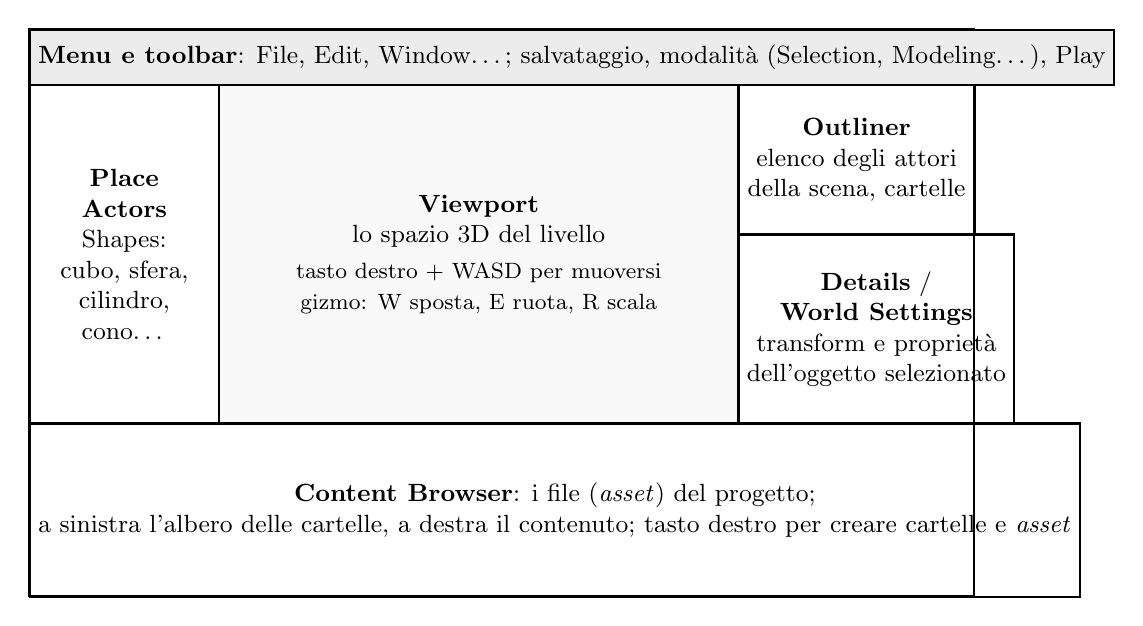
\begin{tikzpicture}[
  font=\small,
  ue1pan/.style={draw, thick, align=center, inner sep=3pt},
  ue1note/.style={font=\footnotesize, align=left, text width=3.4cm}
]
  % cornice
  \draw[thick] (0,0) rectangle (12,7.2);
  % toolbar
  \node[ue1pan, minimum width=12cm, minimum height=0.7cm, anchor=north west, fill=gray!15]
    at (0,7.2) {\textbf{Menu e toolbar}: File, Edit, Window\ldots; salvataggio, modalità
    (Selection, Modeling\ldots), Play};
  % place actors
  \node[ue1pan, minimum width=2.4cm, minimum height=4.3cm, anchor=north west]
    at (0,6.5) {\textbf{Place}\\\textbf{Actors}\\Shapes:\\cubo, sfera,\\cilindro,\\cono\ldots};
  % viewport
  \node[ue1pan, minimum width=6.6cm, minimum height=4.3cm, anchor=north west, fill=gray!5]
    at (2.4,6.5) {\textbf{Viewport}\\lo spazio 3D del livello\\[2pt]
    \footnotesize tasto destro + WASD per muoversi\\\footnotesize gizmo:
    W sposta, E ruota, R scala};
  % outliner
  \node[ue1pan, minimum width=3cm, minimum height=1.9cm, anchor=north west]
    at (9,6.5) {\textbf{Outliner}\\elenco degli attori\\della scena, cartelle};
  % details
  \node[ue1pan, minimum width=3cm, minimum height=2.4cm, anchor=north west]
    at (9,4.6) {\textbf{Details} /\\\textbf{World Settings}\\transform e proprietà\\
    dell'oggetto selezionato};
  % content browser
  \node[ue1pan, minimum width=12cm, minimum height=2.2cm, anchor=north west]
    at (0,2.2) {\textbf{Content Browser}: i file (\emph{asset}) del progetto;\\
    a sinistra l'albero delle cartelle, a destra il contenuto; tasto destro per creare
    cartelle e \emph{asset}};
\end{tikzpicture}
\caption{Una disposizione tipica dell'editor, come quella mostrata da Igor. Ogni pannello
si può spostare, agganciare ad altri o chiudere; il menu Window li riapre.}
\label{ue1:fig:editor}
\end{figure}

\paragraph{Le cartelle, e i loro colori.} Nel Content Browser, con il \textbf{tasto
destro}, si possono creare vari tipi di \emph{asset}; per cominciare, una cartella:
\textbf{New Folder}, chiamata ``prova''. Si possono creare tutte le cartelle che si
vogliono, ``in modo da avere ordine''. Una ``piccola chicchetta'': con il tasto destro
su una cartella, \textbf{Set Color}, la si può \textbf{colorare} (Igor la fa blu), un
feedback visivo che rende la navigazione molto più veloce. Il Content Browser mostra le
cartelle in due modi: a destra come in un \emph{explorer}, a sinistra come un albero ``a
cascata''. Se si mette una cartella dentro un'altra, a sinistra compare una piccola
freccia che apre la cartella sottostante: cartelle e sottocartelle.

\paragraph{L'ordine, per sé e per gli altri.} ``È molto importante l'organizzazione.'' Le
cartelle si riempiranno di \emph{asset}, e bisognerà cercarne uno solo senza sapere dove
andare. L'ordine serve ``non solo per la salvezza vostra, ma anche dei vostri possibili
collaboratori'': ``vi assicuro che quando siete ordinati, la gente vi ringrazia''.

\paragraph{Approfondimento: il Content Drawer e la definizione di \emph{asset}.} Nella
disposizione predefinita di Unreal Engine 5 il Content Browser non è sempre aperto: lo si
richiama dal pulsante \textbf{Content Drawer} in basso a sinistra (o con
Ctrl+Spazio), e lo si può agganciare stabilmente all'interfaccia (``Dock in Layout''),
come ha fatto Igor. Romero e Sewell definiscono l'\emph{asset} come ``un pezzo di
contenuto di un progetto Unreal'': materiali, \emph{static mesh} e Blueprint sono tutti
\emph{asset}. Quando si trascina un \emph{asset} dal Content Browser nel livello,
l'editor ne crea una \textbf{copia} da piazzare nella scena: l'\emph{asset} resta uno, le
sue istanze nel livello possono essere molte. Gli stessi autori descrivono l'Outliner
come l'elenco degli oggetti presenti nel livello, e i Details come il pannello che
mostra le proprietà modificabili dell'oggetto selezionato.

% ---------------------------------------------------------------------
\section{Il primo cubo e il \emph{transform}}
\label{ue1:sec:transform}

\paragraph{Place Actors.} Gli \emph{actor} sono gli elementi di gioco. Dal pannello
\textbf{Place Actors} (se manca: Window, Place Actors), nella sezione \textbf{Shapes},
si prende un \textbf{cubo} e lo si trascina nella viewport. ``Ecco a voi un cubetto
renderizzato'': il primo cubo in Unreal, ``e ne avrete tanti''.

\paragraph{I tre assi.} Sul cubo compaiono tre frecce: sono i tre assi principali,
\textbf{X}, \textbf{Y} e \textbf{Z}, lungo i quali lo si può muovere. Ogni asse ha il
suo colore: \textbf{X rosso}, \textbf{Y verde}, \textbf{Z blu}.

\paragraph{Il \emph{transform}.} Di ogni oggetto si possono modificare
\textbf{locazione}, \textbf{rotazione} e \textbf{scala}. L'insieme dei tre è il
\textbf{\emph{transform}} (``quando parleremo di \emph{transform}, ricordatevelo''), e
lo si rivedrà ``a oltranza''. Lo si modifica in due modi: con le frecce nella viewport,
o con i numeri nel pannello \textbf{Details}.

\paragraph{I numeri nei Details.} Nei Details la locazione del cubo è, per esempio, 480,
430, 120: è la \textbf{raffigurazione numerica}, in unità di Unreal, del punto in cui si
trova l'oggetto. Se si scrive 0 al posto del primo valore e si preme Invio, ``poplà'':
la coordinata X del cubo adesso è 0. Se si trascina una freccia guardando i numeri, si
vede il valore crescere o diminuire, andare in positivo o in negativo: è il verso
dell'asse.

\paragraph{Unreal ragiona in centimetri.} ``Molto importante'': \textbf{l'unità di Unreal
è il centimetro}. Se un oggetto va spostato di tre metri, lo si sposta di 300 unità.
Nella griglia del pavimento ogni riquadro, dice Igor, è un metro, e un cubo, di
default, è un metro.

\paragraph{W, E, R.} Il \textbf{pivot} (o \emph{gizmo}) è ``questo cosettino degli
assi'', e permette tre movimenti: con \textbf{W} si sposta (locazione), con \textbf{E} si
ruota, con \textbf{R} si scala. Gli stessi tre strumenti sono anche in alto a destra
nella viewport, come icone.

\paragraph{Assi locali e assi globali.} Esistono due riferimenti: gli assi
\textbf{relativi} all'oggetto stesso (\textbf{locali}) e quelli del \textbf{mondo}
(\textbf{globali}, la sua \emph{absolute location}). Finché il cubo non è ruotato la
differenza non si vede; ma se lo si ruota fino a farlo diventare ``una specie di rombo''
e si infila nel terreno, alzarlo lungo i suoi assi locali richiede ``un doppio
movimento, così e così'', perché gli assi locali ruotano insieme a lui (``avremo il
nostro bel pivot ruotato di 40 gradi''). Con gli assi globali, invece, l'alto è sempre
l'alto. Il passaggio dall'uno all'altro si fa con l'icona in alto nella viewport:
\textbf{il cubetto con tre assi} indica il riferimento \textbf{locale}, \textbf{il
mondo} indica quello \textbf{globale}. La scelta vale per locazione e rotazione.

\paragraph{La scala è solo locale.} Non vale per la scala: \textbf{un oggetto si può
scalare solo nei suoi assi locali}. Se si scalasse un oggetto ruotato lungo gli assi del
mondo, ``verrebbe totalmente stretchato malissimo'': l'oggetto è girato in un modo e
l'asse in un altro, e allungarlo così lo deformerebbe. Unreal ``ce lo impedisce''.

\paragraph{Le unità di misura del \emph{transform}.} La locazione è in centimetri, la
\textbf{rotazione in gradi} (``io l'ho ruotato e c'è un 40''), la \textbf{scala in
unità}: 1 è la dimensione originale, 2 il doppio.

\begin{figure}[htbp]
\centering
\begin{tikzpicture}[
  font=\small,
  ue1ax/.style={-{Stealth[length=3mm]}, very thick},
  ue1box/.style={draw, thick, rounded corners=3pt, text width=3.6cm, align=left,
               inner sep=5pt}
]
  % assi
  \coordinate (o) at (0,0);
  \draw[ue1ax, red!75!black] (o) -- (2.2,0) node[right]{X};
  \draw[ue1ax, green!50!black] (o) -- (1.2,1.1) node[above right]{Y};
  \draw[ue1ax, blue!75!black] (o) -- (0,2.2) node[above]{Z};
  \fill (o) circle (2pt);
  \node[below=0.2cm of o, font=\footnotesize, align=center]
    {pivot: X rosso, Y verde, Z blu};
  % riquadri
  \node[ue1box, right=2.8cm of o, yshift=1.6cm] (loc)
    {\textbf{Location} (\textbf{W})\\in centimetri\\locale o globale};
  \node[ue1box, below=0.25cm of loc] (rot)
    {\textbf{Rotation} (\textbf{E})\\in gradi\\locale o globale};
  \node[ue1box, below=0.25cm of rot] (sca)
    {\textbf{Scale} (\textbf{R})\\in unità (1 = originale)\\solo locale};
  \node[draw, thick, dashed, fit=(loc)(rot)(sca), inner sep=6pt,
    label={[font=\small\bfseries]above:Transform}] {};
\end{tikzpicture}
\caption{Gli assi e il \emph{transform}. Lo \emph{snapping} (sezione
\ref{ue1:sec:snap}) si imposta separatamente per ognuna delle tre componenti.}
\label{ue1:fig:transform}
\end{figure}

\paragraph{Il tasto Fine.} Un'altra ``piccola chicchetta'': se si piazza un cubo in
aria e si preme il tasto \textbf{Fine} (\emph{End}, quello ``sopra le frecce''), il cubo
cade sulla prima superficie che trova sotto di sé. ``Molto utile'', perché evita di
stare lì ad abbassarlo a occhio.

\paragraph{I Details seguono la selezione.} Ogni volta che si clicca un oggetto, i Details
mostrano \emph{quell'}oggetto: due cubi hanno due locazioni, due rotazioni, due scale.
\textbf{Per modificare i parametri di un oggetto, bisogna selezionarlo.}

\paragraph{Lavorare con i numeri.} I numeri dei Details sono lo strumento preciso, e
sono molto usati, per esempio, dai level designer: ``dobbiamo allargare il corridoio di
tre metri''. Igor allunga un cubo di tre metri sull'asse Y. Nei campi numerici si può
anche scrivere, oppure \textbf{trascinare}: si mette il mouse sul campo e lo si fa
scorrere a destra e a sinistra (``slidando'') per cambiare il valore, su qualunque asse,
per locazione, rotazione e scala.

\paragraph{Reset.} Accanto a ogni gruppo di valori c'è una \textbf{freccetta}: cliccandola,
il valore torna a quello originale (la scala torna a 1, la locazione al punto di
partenza).

% ---------------------------------------------------------------------
\section{Muoversi, duplicare, raggruppare}
\label{ue1:sec:navigazione}

\paragraph{Forme e pivot.} Si possono piazzare tanti \emph{actor} diversi: cilindri,
coni, sfere. Il pivot è al \textbf{centro} di ogni figura, e per questo un cilindro,
appena piazzato, è ``mezzo interrato''. Per \textbf{scalare su tutti gli assi
insieme} si prende il centro del gizmo di scala e si trascina verso l'esterno (allarga)
o verso l'interno (stringe); trascinando una sola maniglia si scala su un solo asse.

\paragraph{Duplicare con Alt.} Igor costruisce un tavolino con un cilindro schiacciato e
uno allungato. Serve un altro pezzo uguale: bisogna prendere un altro cilindro e rifare
tutto? No: \textbf{si tiene premuto Alt e si trascina} (o si ruota) l'oggetto, e se ne
crea una copia esatta. ``Lo userete a manetta.'' Funzionano anche \textbf{Ctrl+C} e
\textbf{Ctrl+V}. Una studentessa, abituata a Blender, si confonde: premeva Alt e lo
lasciava. Alt va \textbf{tenuto premuto mentre si trascina}, ``non è solo \emph{tap}
Alt''.

\paragraph{Muoversi nella viewport.} ``Mi sono dimenticato di dirvelo, perdonatemi'':
per muoversi nella viewport si tiene premuto il \textbf{tasto destro} del mouse e si
usano \textbf{W, A, S, D}, come in un gioco in prima persona; muovendo il mouse si
ruota la camera. Uno studente scopre da solo che \textbf{E} sale e \textbf{Q} scende:
``bravissimo, esatto''. Bisogna cliccare dentro la viewport: è la camera dell'editor,
non quella del gioco.

\paragraph{Seguire un oggetto.} Se si tiene premuto \textbf{Shift} mentre si trascina un
oggetto, la camera lo \textbf{segue} nel movimento: utile per piazzamenti
particolari.

\paragraph{Selezionare più oggetti.} Per selezionare più oggetti si tiene premuto
\textbf{Shift} (o Ctrl) e si cliccano uno dopo l'altro. Con il palo e il piano del
tavolo selezionati, Alt e trascinamento: ``pac!'', un secondo tavolino.

\paragraph{I gruppi.} Selezionare ogni volta tutti i pezzi è scomodo, perché se si
clicca il piano del tavolo si seleziona solo il piano. Si possono allora
\textbf{raggruppare}: si selezionano gli oggetti, tasto destro, \textbf{Group}, oppure
\textbf{Ctrl+G}. Intorno al gruppo compare ``una specie di reticolo verde'', e cliccando
un pezzo qualunque si seleziona il tutto. Si possono anche raggruppare dei gruppi, per
farne uno più grande. Per \textbf{sciogliere} un gruppo: \textbf{Shift+G}, oppure tasto
destro, Groups, \textbf{Ungroup}.

\paragraph{Ctrl+Z.} ``Qua funziona'': \textbf{Ctrl+Z} annulla. ``Sappiatelo, ogni
errore può essere cancellato, o almeno per poco.''

\paragraph{I gruppi non sono un oggetto unico.} Igor fa vedere un limite: se si
\textbf{scala} un gruppo, Unreal non lo scala come un oggetto unico; ogni pezzo si
scala rispettando i propri assi relativi. Per avere un oggetto davvero unico bisognerà
creare una \textbf{static mesh}, ``che vedremo in seguito''.

\paragraph{Mesh e static mesh.} Una \textbf{mesh} è un oggetto solido formato da
poligoni: quando qualcuno dice ``mi serve la mesh del tavolo'' intende il
\textbf{modello 3D} del tavolo. La \textbf{static mesh} è un tipo di mesh; esistono anche
le \textbf{dynamic mesh}, ``un discorso che vedremo più avanti''.

\paragraph{Approfondimento: \emph{transform} relativi nei Blueprint.} Il comportamento dei
gruppi anticipa un tema che nei Blueprint tornerà spesso. Romero e Sewell, nel capitolo
sui nodi matematici, distinguono il \textbf{\emph{transform} del mondo} di un attore
(la sua posizione assoluta nel livello) dal \textbf{\emph{transform} relativo} dei suoi
componenti, che è relativo al componente ``genitore''. Il loro esempio è un tavolo con
sopra una statua: se si sposta il tavolo, la statua lo segue; se si cambia il
\emph{transform} relativo della statua, il tavolo resta dov'è. È il modo in cui, dentro
una Blueprint Class, si costruiscono oggetti composti che si muovono come un tutt'uno.

% ---------------------------------------------------------------------
\section{Lo \emph{snapping} e la velocità della camera}
\label{ue1:sec:snap}

\paragraph{Lo \emph{snapping}.} Ruotando un oggetto, l'editor mostra un numero che sale
a scatti: 20, 30, 40, 50, 60, 70 gradi. È lo \textbf{\emph{snap}}, che si controlla in
alto a destra nella viewport: ci sono tre pulsanti, per locazione, rotazione e scala,
ognuno con un valore. \textbf{Se il pulsante è azzurro, lo \emph{snap} è attivo.}
\begin{itemize}
  \item Senza \emph{snap} di rotazione l'oggetto ruota liberamente, con i decimali; con
        lo \emph{snap} a 10, ruota di dieci gradi alla volta. Cliccando sul numero si
        sceglie il passo: 5, 10, 15, 30, 45, 60, 90, 120 gradi. Con 120, ``pam!'',
        diretto da 0 a 120; con 5, una rotazione più fine.
  \item Lo stesso vale per la \textbf{locazione}: con lo \emph{snap} l'oggetto si muove
        ``a scattini'' (di 1, 5, 10, 50 unità\ldots), senza si muove di qualunque
        valore, decimali compresi.
  \item E per la \textbf{scala}: senza \emph{snap} si scala ``quanto mi pare'', con lo
        \emph{snap} a passi anche molto piccoli, come 0,25.
\end{itemize}
Se lo \emph{snapping} impedisce di mettere un pezzo dove si vuole, ``basta
disattivarlo''.

\paragraph{La velocità della camera.} Per raggiungere ``quella montagna là'' si può
\textbf{velocizzare la camera}: mentre ci si muove (tasto destro premuto), si gira la
\textbf{rotellina del mouse} in avanti per andare più veloci e indietro per andare più
lenti, quando bisogna osservare un oggetto da vicino con precisione (Igor scende fino a
una velocità di 0,03 per guardare sotto il tavolino).

% ---------------------------------------------------------------------
\section{L'Outliner e l'ordine della scena}
\label{ue1:sec:outliner}

\paragraph{L'elenco della scena.} L'\textbf{Outliner} (se manca: Window, Outliner) è una
raffigurazione a lista di \textbf{tutti gli oggetti in scena}. Se si duplica un cono,
nell'Outliner compaiono Cone, Cone2, Cone3, Cone4\ldots{} Un oggetto si può selezionare
sia nella viewport sia nell'Outliner, ed è utile quando ``avete un bel \emph{pack} di
roba'' da gestire. Per eliminare un oggetto: \textbf{Canc} (\emph{Delete}).

\paragraph{Le cartelle dell'Outliner.} Anche nell'Outliner si possono creare cartelle, e
a Igor ``aiuta molto'' nella pianificazione e nel piazzamento. Tasto destro
nell'Outliner, \textbf{Create Folder}, e si crea una cartella ``Coni''. Poi si
selezionano i coni: visto che sono elencati per nome, si clicca il primo, si tiene
premuto \textbf{Shift} e si clicca l'ultimo, e si seleziona tutta la lista; si
trascinano dentro la cartella. Da quel momento, invece di cliccarli uno per uno, basta
il tasto destro sulla cartella e \textbf{Select All Descendants}: ``eccoli qua''.

\paragraph{Perché farlo subito.} ``Immaginatevi una scena intera, gigantesca.'' Senza
ordine si passano ``tre quarti d'ora'' a cliccare un oggetto dopo l'altro; con le
cartelle, un tasto e si è fatto. ``Vi risparmiate molto tempo.''

\paragraph{Il tasto G.} Un ultimo tasto, che Igor spiega durante la dimostrazione: se il
pivot ``scompare'', bisogna premere \textbf{G}. G passa dalla visualizzazione
dell'editor, con gli aiuti visivi, a quella ``normale'' del mondo di gioco, in cui gli
aiuti sono nascosti.

\paragraph{Approfondimento: la Game View.} Il comando si chiama \textbf{Game View}: con G
la viewport mostra la scena come la vedrebbe il giocatore, nascondendo icone,
\emph{gizmo} e oggetti che nel gioco sono invisibili (le icone delle luci, i volumi, i
punti di partenza del giocatore). È comodo per giudicare l'aspetto finale di una scena;
ma se lo si attiva per sbaglio sembra che gli strumenti siano spariti, ed è per questo
che Igor lo nomina proprio quando il pivot ``scompare''.

\begin{table}[htbp]
\centering
\small
\begin{tabular}{@{}p{4.3cm}p{8.7cm}@{}}
\toprule
\textbf{Comando} & \textbf{Che cosa fa} \\
\midrule
Tasto destro + W A S D & muoversi nella viewport; con il mouse si ruota la camera \\
Tasto destro + E / Q & salire / scendere \\
Rotellina (durante il movimento) & velocità della camera: avanti più veloce, indietro
  più lenta \\
W / E / R & gizmo di locazione / rotazione / scala \\
Icona cubetto / mondo & assi locali / globali (per locazione e rotazione) \\
Pulsanti azzurri dello \emph{snap} & attivano lo \emph{snapping} e ne scelgono il
  passo \\
Fine (\emph{End}) & fa cadere l'oggetto sulla superficie sottostante \\
Alt + trascinamento & duplica l'oggetto (Alt tenuto premuto) \\
Ctrl+C / Ctrl+V & copia e incolla \\
Shift + clic & selezione multipla; nell'Outliner, selezione di un intervallo \\
Shift + trascinamento & la camera segue l'oggetto \\
Ctrl+G / Shift+G & raggruppa / separa (anche: tasto destro, Groups) \\
Ctrl+Z & annulla \\
Canc (\emph{Delete}) & elimina l'oggetto selezionato \\
G & Game View: mostra o nasconde gli aiuti dell'editor \\
Freccetta accanto ai valori & riporta il valore all'originale \\
Ctrl+S & salva \\
\bottomrule
\end{tabular}
\caption{I comandi della prima lezione. Tutti valgono nel Level Editor di Unreal Engine
5.5 con le impostazioni predefinite.}
\label{ue1:tab:comandi}
\end{table}

% ---------------------------------------------------------------------
\section{Esercitazione: il ristorante dei tre tavoli}
\label{ue1:sec:esercitazione}

Con quello che si è imparato, ``una piccola esercitazione''. Bisogna costruire, con le
forme di base, \textbf{tre tavoli con le loro sedie}:
\begin{enumerate}
  \item un tavolo con \textbf{tre posti}: ``vengono tre ospiti a cena'';
  \item un \textbf{tavolo quadrato} per \textbf{cinque ospiti};
  \item una \textbf{cena romantica}: un tavolo per \textbf{due}, ``e se volete
        metteteci pure la candela''.
\end{enumerate}
Non serve una sedia precisa: ``l'importante è che applicate tutto quello che abbiamo
fatto''. Chi non riesce oggi può farlo per la volta successiva (``assolutamente''), e
riguardare la registrazione.

\paragraph{Partire da una reference.} Un consiglio, ``soprattutto per voi artisti'': per
fare qualcosa di artistico, prendere una \textbf{reference}. Ma non una sedia troppo
complessa: ``non ci interessa fare una cosa bella e bellissima''. Igor sceglie una
sedia ``molto semplice'', la ``sedia della nonna che vi fa il ragù''.

\paragraph{La dimostrazione.} Igor costruisce la sua sedia passo per passo, ed è un buon
riassunto di tutta la seconda parte:
\begin{enumerate}
  \item un cubo, scalato con lo \emph{snap} a 0,25, per la seduta; la freccetta di reset
        per riportarlo alle dimensioni di partenza quando serve (``le sedie sono alte
        più o meno un metro'');
  \item la prima gamba, posizionata (``se avete problemi con lo \emph{snapping}, basta
        disattivarlo'');
  \item le altre gambe: Shift per selezionare, Alt per duplicare. Ne viene ``questo
        bellissimo sgabello'', con le gambe ``non proprio precisissime'';
  \item lo schienale, duplicando altri pezzi per il dorso;
  \item tutti i pezzi selezionati e \textbf{Ctrl+G}, ``perché sennò dobbiamo fare ogni
        volta uno, due, tre, quattro'';
  \item la sedia accostata al tavolo (``è un po' spesso questo tavolo, ci saranno delle
        ginocchiate incredibili, ma non ci importa'').
\end{enumerate}

\paragraph{Si può allineare un oggetto a un altro?} Uno studente, che oggi può solo
guardare, chiede se c'è un modo di allineare le gambe della sedia a un oggetto, visto
che a mano non è semplice. Igor risponde che non è una cosa che in Unreal si fa
``professionalmente'': strumenti di allineamento precisi ci sono nei programmi di
modellazione, come Blender e Maya. In Unreal ci sono il tasto \textbf{Fine}, lo
\emph{snapping}, il lavoro ``un po' a mano'', i \emph{plugin}, oppure la
\textbf{Modeling Mode}, la modalità di modellazione dell'editor, con strumenti più
precisi, che si vedrà in seguito.

\paragraph{Gli strumenti si somigliano.} Lo stesso studente nota che, in attesa del
download, ha usato \textbf{Inkarnate}, un programma per disegnare mappe, e che i
principi visti finora sono ``molto simili''. ``Sì, assolutamente'': sono principi
condivisi dai vari game engine e dai programmi grafici. In Unity ``magari qualche
bottone è un po' diverso'', ma le funzioni sono simili; ``si impara a muoversi da una
parte e si impara a muoversi dall'altra''. Igor mostra anche \textbf{Dungeon
Scrawl}\footnote{Igor ci arriva per tentativi: ``Dungeon Crawler'', ``Dungeon
Designer'', ``Dungeon Scroll''.}, uno strumento per disegnare mappe per le partite di
D\&D con gli amici, usato anche per il level design.

\paragraph{I risultati.} Dopo una ventina di minuti di lavoro individuale, i
``ristoratori in erba'' mostrano i loro tavoli.
\begin{itemize}
  \item Uno studente ha aggiunto una \textbf{luce} per la candela, ma la candela fa
        ombra. Igor gli mostra come risolvere: si seleziona la luce e nei Details, in
        basso, si toglie la spunta a \textbf{Cast Shadows}.
  \item Qualcuno ha fatto un tavolo rettangolare invece che quadrato: ``va benissimo,
        tranquilli''.
  \item Uno studente, che ha appena finito il download, ha fatto solo la base del tavolo
        e una gamba della sedia, sottilissima. Igor ricorda che Unreal lavora in
        centimetri, e quella gamba è di pochi centimetri: ``non ci farei sedere
        nessuno, potrebbe crollare''. Ma ``è soggettivo''.
\end{itemize}
``A parte l'ironia'', la conclusione è che gli oggetti in sé contano poco: conta capire
come ci si muove in Unreal, duplicando, scalando, muovendo, ruotando. ``Questa è la cosa
più importante che oggi impariamo.''

\paragraph{Una cartella per ogni tavolo.} Un'ultima richiesta: mettere ogni gruppo in una
cartella dell'Outliner. Create Folder, ``Tavolo da due'', si selezionano i pezzi e li si
trascina dentro; poi ``Tavolo da tre'', e così via. Con Select All Descendants si
riprende il tavolo intero in un clic.

% ---------------------------------------------------------------------
\section{Salvare la mappa, e la chiusura}
\label{ue1:sec:chiusura}

\paragraph{Salvare.} Per salvare il lavoro c'è il classico \textbf{Ctrl+S}. Siccome la
mappa è stata creata ``da nulla'', la prima volta Unreal chiede dove salvarla: le si dà
un nome (``MappaProva'') e la si salva dentro la cartella ``prova'' del Content
Browser. In basso a destra, poi, l'editor tiene il conto delle modifiche non salvate:
se si sposta anche solo una sedia, compare l'indicazione degli oggetti
\textbf{\emph{unsaved}}, ``tutti gli oggetti che devo salvare''.

\paragraph{Che cos'è il secondo file?} Uno studente nota che il salvataggio crea anche un
secondo file, un \textbf{HLOD Layer}\footnote{Nella trascrizione ``Halodle'' e ``Halod
Layer''.}. Igor spiega che dipende dalla mappa: quella su cui hanno lavorato contiene un
\textbf{landscape}, le montagne che si vedono in fondo. Il landscape è un piano che si
può modellare con uno strumento apposito per formare, per esempio, il paesaggio di
sfondo; il file salva come quel piano è composto. La volta successiva si userà una
mappa davvero vuota, senza landscape.

\paragraph{Approfondimento: LOD e HLOD.} \textbf{LOD} sta per \emph{level of detail}:
lo stesso oggetto esiste in più versioni, con un numero decrescente di poligoni, e
l'engine usa quelle più semplici quando l'oggetto è lontano dalla camera, dove i
dettagli non si vedrebbero comunque. È la risposta pratica al compromesso della
sezione~\ref{ue1:sec:rendering} tra precisione e peso. Gli \textbf{HLOD}
(\emph{hierarchical} LOD) fanno lo stesso a livello di gruppi: interi blocchi lontani
della mappa vengono sostituiti da un'unica versione semplificata. Le mappe ``a mondo
aperto'' di Unreal Engine 5, con il landscape, li usano per impostazione predefinita, ed
è per questo che il salvataggio crea un file di \emph{HLOD Layer}.

\paragraph{Le ultime domande.} Come si separano gli oggetti raggruppati? ``Shift+G, oppure
tasto destro, Ungroup: se lo cerchi c'è proprio scritto.'' Quando arriva la
registrazione? Sul sito, ``credo il giorno dopo''. Le foto dei lavori si possono mandare
a Igor su Discord, ``tranquillamente'' (``quando ci sono, vi rispondo''), anzi in un
\emph{thread} o un canale apposito, ``così almeno è più ordinato e non mi riempite la
casella privata''.

\paragraph{Il calendario.} Giovedì si rivede Igor; il martedì successivo c'è Davide, con
la parte artistica; poi le lezioni si alternano, ``settimana a settimana''. Sono le 19:
``per chi tra poco cena, auguro buona cena a tutti''. ``Se avete domande, fatele adesso o
tacete fino alla prossima volta.'' ``Ciao, ragazzi.''

% ---------------------------------------------------------------------
\section*{Punti chiave del capitolo}
\addcontentsline{toc}{section}{Punti chiave del capitolo}

\begin{itemize}
  \item Il \textbf{game engine} è ``il calderone'' che riunisce 3D art, programmazione e
        design in un unico ambiente, con fisica e collisioni, suono, animazione,
        networking e IA. Lo si governa con lo \textbf{scripting}; in Unreal, con i
        \textbf{Blueprint}, un linguaggio a nodi usato anche dai programmatori (il C++
        resta per ottimizzare). Conta la \textbf{logica}, più dello strumento.
  \item Il \textbf{rendering} trasforma poligoni in pixel: \textbf{\emph{vertex
        shading}} (i vertici dei triangoli), \textbf{rasterizzazione} (quali pixel),
        \textbf{\emph{fragment shading}} (colore, luce, ombre, riflessi). Più poligoni
        = più precisione, ma più peso: ``un cubo con due milioni di poligoni'' fa
        esplodere il gioco.
  \item Il \textbf{\emph{real time rendering}} lavora tra 20 e 120 \emph{fps}: il cinema
        è a 24, il gaming a 30--60 e oltre. Un \textbf{frame} è un'immagine; la loro
        successione dà l'illusione del movimento.
  \item Unreal è il più usato perché è un \textbf{linguaggio comune}, aggiornato di
        continuo, e perché permette di \textbf{prototipare} subito: ``non ci interessa
        se è bello o brutto, è importante che funzioni'' (il prototipo di
        \emph{Expedition 33}). È usato anche nel cinema, dove conta il dettaglio più
        dell'ottimizzazione.
  \item Ciò che distingue un videogioco da un video è il \textbf{game loop}: input,
        \emph{update}, render, e di nuovo, a ogni \emph{frame}.
  \item \textbf{Ogni buona idea non esiste finché non sta su carta.} Indie, AA e AAA si
        distinguono per i soldi e per la specializzazione dei ruoli (fino ai \emph{leaf
        artist}). L'\textbf{\emph{outsourcing}} è chiedere a un altro studio una parte
        del lavoro, senza cedergli la proprietà.
  \item Tutti i ruoli toccano l'engine: \emph{blockout} e metriche per il level
        designer, momenti scriptati per il narrative designer, parametri esposti per il
        combat designer, materiali e Sequencer per gli artisti, rendering, IA e rete per
        i programmatori, Unreal Insights per il QA. \textbf{Trattate bene i vostri
        programmatori.}
  \item Un gioco è fatto di \textbf{attori, meccaniche, spazio, obiettivi, regole} (e a
        volte \textbf{tempo}); il divertimento è una \textbf{conseguenza}, e il gameplay
        nasce dalle \textbf{scelte}. Meccanica = che cosa posso fare; dinamica = come lo
        faccio; estetica = come mi fa sentire. ``Un gioco per tutti non è un gioco per
        nessuno.''
  \item Il bilanciamento è un lavoro tra \textbf{designer e QA}; il feedback utile è
        quello da cui si ricava un'informazione. Far giocare chi non ha mai visto il
        gioco ``è la cosa più pura''.
  \item Per il corso serve Unreal \textbf{5.5} (la 5.5.4): l'ultimo numero è solo
        l'aggiornamento, il secondo decide la compatibilità.
  \item Le risorse: \textbf{documentazione}, forum, corsi gratuiti di
        \emph{learning}, \textbf{Fab} con i \emph{pack} gratuiti del mese (``prendeteli
        sempre''). Ma \textbf{prima la funzione, poi l'\emph{asset}}, o il progetto
        pesa 70~GB per usarne tre.
  \item Quando si preme Play gli attori vengono inizializzati e duplicati. Ogni
        movimento va reso \textbf{relativo al tempo di gioco} (\emph{delta seconds}),
        altrimenti dipende dagli \emph{fps}.
  \item Il progetto di prova: Games, \textbf{Blank}, Blueprint, Desktop, Starter
        Content, nome \textbf{senza spazi}. I template si distinguono per le
        \textbf{3C}: camera, controller, character.
  \item L'editor è fatto di \textbf{finestre} spostabili (Window le riapre): viewport,
        Details, Outliner, World Settings, \textbf{Content Browser}. Cartelle colorate
        e ordine: ``quando siete ordinati, la gente vi ringrazia''.
  \item Il \textbf{transform} è locazione (\textbf{centimetri}), rotazione
        (\textbf{gradi}) e scala (\textbf{unità}); \textbf{W, E, R}; X rosso, Y verde,
        Z blu; assi locali o globali, ma \textbf{la scala è solo locale}.
  \item \textbf{Alt + trascinamento} duplica, \textbf{Ctrl+G} raggruppa, \textbf{Fine}
        appoggia a terra, lo \textbf{\emph{snap}} azzurro fa muovere a scatti, la
        \textbf{rotellina} cambia la velocità della camera, \textbf{Select All
        Descendants} riprende un'intera cartella dell'Outliner.
\end{itemize}

%
%  Tutte le etichette di questo capitolo hanno il prefisso "ue1:"
%  (ue1:cap:..., ue1:sec:..., ue1:fig:..., ue1:tab:...), e tutti gli
%  stili TikZ hanno il prefisso "ue1" (ue1box, ue1arr, ...) per non
%  collidere con chiavi native di TikZ. Il capitolo è autonomo: non
%  contiene \ref verso altri capitoli.
%  Le figure sono ricostruzioni schematiche di quanto mostrato e detto a
%  lezione, non copie delle slide del docente. Dove la trascrizione è
%  troppo rovinata per ricostruire un dettaglio, il capitolo lo dice
%  invece di inventarlo.
% =====================================================================

\chapter[Introduzione a Unreal Engine]{Introduzione a Unreal Engine: che cos'è un
engine, chi lo usa, e il primo contatto con l'editor}
\label{ue1:cap:intro}

Questa è la \textbf{prima lezione} del corso breve di \textbf{introduzione a Unreal
Engine}, un corso che ha il suo centro nei \textbf{Blueprint}, il sistema di
programmazione visuale ``a nodi'' dell'engine di Epic Games. La lezione ha due metà
molto diverse. La prima è teorica e larga: che cos'è un \emph{software}, che cos'è un
\emph{game engine}, come un modello fatto di poligoni diventa un'immagine sullo
schermo, perché Unreal è oggi l'engine più diffuso, quali figure di una produzione lo
usano e per che cosa, e infine, con un'attività in classe, da che cosa è formato un
gioco. La seconda metà è pratica: si scarica Unreal Engine 5.5, si guardano le risorse
che Epic mette a disposizione (la documentazione, i corsi gratuiti, il negozio di
\emph{asset} Fab), si crea un primo progetto vuoto e si impara a muoversi nell'editor:
piazzare un cubo, spostarlo, ruotarlo, scalarlo, duplicarlo, raggrupparlo, ordinarlo
in cartelle. La lezione si chiude con un'esercitazione: arredare un piccolo
ristorante con tre tavoli e le loro sedie.

Il docente è \textbf{Igor}\footnote{Il docente si presenta come ``Igor Ripanti''; il
cognome è quello della trascrizione automatica, che altrove storpia quasi tutti i nomi
propri, e il capitolo non è in grado di verificarlo.}, che si presenta come ex alunno
della stessa scuola degli studenti, ``precisamente per quanto riguarda game
design''\footnote{La trascrizione dice ``sono stato un alunno di Live'': il nome della
scuola è con ogni probabilità storpiato.}. Ha lavorato a \textbf{\emph{Steel Seed}},
``principalmente come \emph{level designer}''; ma ``essendo un ambiente indie'' faceva
``un po' di tutto'', anche programmazione e \emph{scripting}, e quindi ha fatto ``uso
intensivo'' di Unreal Engine ``e di tutte le sue feature''. Il corso è diviso tra due
docenti: con Igor la parte di programmazione e di ``piccole feature''; con
\textbf{Davide}, a partire dal 26 del mese, una parte ``un po' più artistica''. Le
lezioni si alternano: il giovedì successivo gli studenti saranno di nuovo con Igor, il
martedì dopo con Davide.

La lezione è \textbf{online}, su Zoom, con un server Discord del corso per i
materiali e le domande; inizia poco dopo le 17 e finisce alle 19, con una pausa di una
decina di minuti verso le 17 e mezza\footnote{Igor, credendo per errore che la lezione
finisse alle 18 (``sono da un altro corso che finiva alle 18''), dopo la pausa annuncia
che ``manca mezz'ora alla fine''; gli studenti lo correggono (``nella mail c'era
scritto'' alle 19), e il docente ha ``un'altra ora'' per la parte pratica.}. Gli
studenti sono tutti \textbf{nuovi iscritti al primo anno}, di corsi diversi: game
design (la maggioranza), narrative design, character animation, 3D art e
programmazione. Il corso breve, in altre parole, è comune a figure che in una
produzione useranno Unreal in modi molto diversi, ed è proprio da questa varietà che
Igor parte.

Tre avvertenze di lettura. La prima: la trascrizione è automatica e storpia moltissimi
nomi. Unreal diventa ``Arreal'', ``Arial Engine'', ``ArrayLange'', ``ArrayLab'',
``Arrival Engine'', ``Arrial'', ``Ariane Engine'', ``Riala'' e ``a Real Engine'';
\emph{Clair Obscur: Expedition 33} è ``Expedition'' e ``Spedisce 33''; Sandfall
Interactive è ``Send Follow Interactive''; \emph{shader} è anche ``scender''. Dove la
ricostruzione è sicura il capitolo usa la forma corretta e, la prima volta, lo segnala
in nota; dove non lo è riporta la forma della trascrizione e lo dice. La seconda: in
più punti la registrazione contiene lunghi blocchi di testo senza senso e ripetuto
(``qual è la risposta che ci può essere?'', ``a parte il plus time\ldots''): sono
artefatti del riconoscimento vocale durante la pausa e i momenti di lavoro
individuale, e il capitolo li ignora. La terza: la seconda metà della lezione è una
dimostrazione dal vivo nell'editor; il capitolo ricostruisce i passaggi da ciò che Igor
dice mentre li fa, e li completa, dove serve, con i nomi esatti dei comandi.

\paragraph{Come leggere questo capitolo.} Il capitolo segue l'ordine della lezione.
Le figure ricostruiscono gli schemi spiegati a voce o sulle slide (la pipeline di
rendering, il \emph{game loop}, gli elementi di un gioco, l'interfaccia dell'editor,
il \emph{transform}); le tabelle riassumono i ruoli della produzione e le scorciatoie
da tastiera della seconda parte. Qua e là, dei paragrafi di \textbf{approfondimento}
collegano la lezione al libro \emph{Blueprints Visual Scripting for Unreal Engine 5}
di Marcos Romero e Brenden Sewell, che sarà il testo di riferimento per questa parte
del libro, e a qualche nozione tecnica generale; sono segnalati come tali e non fanno
parte della lezione.

Il percorso del capitolo:
\begin{enumerate}
  \item le presentazioni e le esperienze degli studenti (sezione
        \ref{ue1:sec:presentazioni});
  \item il \textbf{software}, il \textbf{game engine} e lo \textbf{scripting}, con i
        Blueprint (sezione \ref{ue1:sec:engine});
  \item il \textbf{rendering 3D}: poligoni, \emph{vertex shading}, rasterizzazione,
        \emph{fragment shading}; poi il \emph{real time rendering} e i \emph{frame}
        (sezioni \ref{ue1:sec:rendering} e~\ref{ue1:sec:realtime});
  \item \textbf{Unreal Engine}: perché è così usato, la prototipazione, i giochi, gli
        engine di una volta, il cinema, il \textbf{game loop} (sezioni
        da~\ref{ue1:sec:unreal} a~\ref{ue1:sec:gameloop});
  \item la \textbf{produzione} e i \textbf{ruoli} che toccano l'engine (sezioni
        \ref{ue1:sec:produzione} e~\ref{ue1:sec:ruoli});
  \item l'attività in classe: \textbf{da che cosa è formato un gioco}, e le domande
        prima della pausa (sezioni \ref{ue1:sec:elementi} e~\ref{ue1:sec:domande});
  \item il \textbf{download} della 5.5, le \textbf{risorse} (documentazione,
        \emph{learning}, Fab) e un po' di teoria sul \emph{Play in Editor} e sul
        \emph{delta time} (sezioni da~\ref{ue1:sec:download} a~\ref{ue1:sec:pie});
  \item il primo contatto con l'\textbf{editor}: il progetto, l'interfaccia, il
        \textbf{transform}, la navigazione, l'organizzazione (sezioni
        da~\ref{ue1:sec:progetto} a~\ref{ue1:sec:outliner});
  \item l'\textbf{esercitazione dei tre tavoli}, il salvataggio e la chiusura (sezioni
        \ref{ue1:sec:esercitazione} e~\ref{ue1:sec:chiusura}).
\end{enumerate}

% ---------------------------------------------------------------------
\section{Presentazioni: chi c'è, e chi ha già aperto un engine}
\label{ue1:sec:presentazioni}

La lezione comincia con qualche minuto di attesa (``aspettiamo cinque, dieci minuti''),
un appello e una richiesta: accendere la webcam, ``così almeno ci vediamo un po' in
faccia''. A chi non ha una webcam Igor suggerisce le applicazioni che trasformano il
telefono in una webcam, ``come se ti facessi una videochiamata'': lui usa di solito
\emph{Iriun}\footnote{Nella trascrizione ``Ingur'' e ``Iruin''; si tratta con ogni
probabilità di \emph{Iriun Webcam}, un'applicazione gratuita che fa esattamente
questo.}. I lavori in corso nell'edificio del docente producono ``rumori molesti'' per
tutta la lezione, e Igor se ne scusa.

Poi il giro di presentazioni: nome, corso, ``un piccolo background''. Tutti sono iscritti
al primo anno; i corsi sono game design, character animation, narrative design (più di
uno), 3D art e programmazione. ``C'è una bella quantità di nuovi compagni di design'',
commenta Igor, ``quindi avremo pane per i nostri denti'', oltre ovviamente a 3D art e
programmazione.

\paragraph{Chi ha già usato un engine?} La domanda successiva è se qualcuno abbia ``mai
aperto un software di \emph{develop} per i videogiochi'': Unity, Godot, ``in
generale''. Qualcuno ha provato Godot; qualcuno un po' di Unity, seguendo un corso
online ``molto veloce'' e facendo ``un paio di giochini'', un \emph{platform} e un clone
di \emph{Flappy Bird}, ``di 3D niente''; qualcuno è ``digiuno'', e qualcun altro ha
lavorato ``con roba presa da Fab''. Igor accoglie tutte le risposte allo stesso modo:
``ci sta assolutamente''. Fab, aggiunge, sarà uno dei temi di oggi, perché è ``una
risorsa incredibile'', soprattutto per le cose gratis, quelle in sconto e i contenuti
gratuiti del mese.

\paragraph{La mentalità prima degli strumenti.} A chi parte da zero Igor dà subito una
rassicurazione che vale per tutto il corso: ``l'importante è avere la mentalità''. In
programmazione, ``molto spesso'' si tratta ``semplicemente'' di imparare a usare gli
strumenti, mentre ``la logica fa da padrone''. Passare da un engine all'altro, o da
nessun engine al primo, è soprattutto ``riabituarsi a un nuovo campo di gioco''.

% ---------------------------------------------------------------------
\section{Software, game engine e scripting}
\label{ue1:sec:engine}

\paragraph{Che cos'è un software.} Igor parte dalla definizione più semplice possibile:
il \textbf{software} è ``quello che non è hardware, fondamentalmente''. È un insieme di
istruzioni, di dati e di programmi con funzionalità precise, che ci permettono di
creare cose: strumenti di 3D art come \textbf{Blender} e \textbf{Maya}, oppure
\emph{engine} come \textbf{Unreal Engine} e \textbf{Unity}.

\paragraph{L'engine come calderone.} Il \textbf{game engine} è ``il calderone, chiamiamolo
un po' così'', che riunisce tutte le facoltà di chi sviluppa (3D art, programmazione,
design) e le mette ``in un ambiente comune'', l'ambiente di sviluppo dell'engine. Gli
engine più noti sono \textbf{Unreal}, \textbf{Unity}, \textbf{Godot} e
\textbf{GameMaker}, e ognuno contiene al suo interno molte funzionalità: i
\textbf{motori fisici}, che gestiscono le \textbf{collisioni}; la gestione dei
\textbf{suoni}; le \textbf{animazioni}; il \textbf{networking}; l'\textbf{intelligenza
artificiale} dei personaggi. Nessuna di queste cose ``si fa da sola'': ci mettono le
mani gli sviluppatori, ``tramite lo \emph{scripting}''.

\paragraph{Lo scripting, e i Blueprint.} Lo \textbf{scripting} è ``la forma di
programmazione che ci permette di entrare in interazione e creare cose all'interno
dell'engine''. Esistono molti linguaggi: Igor cita il \textbf{C}, il \textbf{C\#}
(quello di Unity) e i \textbf{Blueprint}, che sono il tipo di \emph{scripting} di Unreal
Engine e l'oggetto di questo corso. Più avanti nella lezione (sezione~\ref{ue1:sec:ruoli})
Igor tornerà sul punto: in Unreal si può programmare anche in codice (in C++), ``ma noi
non lo useremo'', perché i Blueprint bastano ``tranquillamente'', sono usati anche dai
programmatori, e ``tanti giochi nel comparto indie'' sono fatti ``solo con Blueprint,
senza mai toccare una riga di codice''. I Blueprint sono un \textbf{linguaggio a nodi}:
``prendiamo proprio e colleghiamo tutti i nodini'' per dare un senso alla
programmazione.

\paragraph{Approfondimento: le due accezioni di ``Blueprint''.} Romero e Sewell, nel
primo capitolo di \emph{Blueprints Visual Scripting for Unreal Engine 5}, fanno notare
che in Unreal la parola \emph{Blueprint} ha due significati. È il nome del
\textbf{linguaggio di scripting visuale} creato da Epic Games; ed è anche il nome di un
\textbf{tipo di oggetto di gioco} creato con quel linguaggio. I Blueprint di questo
secondo tipo sono di due specie: il \textbf{Level Blueprint}, uno per ogni livello del
gioco (non se ne possono creare altri separati), e le \textbf{Blueprint Class}, che
servono a creare oggetti interattivi riutilizzabili in qualunque livello. Un progetto di
Unreal Engine 5, aggiungono gli autori, si può sviluppare in Blueprint, in C++ o in una
combinazione dei due: si può aggiungere codice C++ a un progetto Blueprint e viceversa.
La scelta di partire dai Blueprint, quindi, non chiude nessuna porta.

% ---------------------------------------------------------------------
\section{Il rendering 3D: dai poligoni ai pixel}
\label{ue1:sec:rendering}

Un'applicazione grafica come un gioco 3D ha una particolarità: il \textbf{3D
rendering}, cioè ``la fase finale dello sviluppo di un'immagine''. È il processo che
prende un \textbf{\emph{3D asset}} (``per il linguaggio un po' più tecnico'') e ci
presenta davanti la scena vera e propria, con gli oggetti creati dai 3D artist ``che
hanno faticato tanto per poterlo fare''. Quegli oggetti sono formati da
\textbf{poligoni}.

\paragraph{Quanti poligoni ha questo oggetto?} Igor chiede se qualcuno ha mai sentito
parlare del numero di poligoni di un modello. Uno studente sì: gli sono capitati ``dei
video di ottimizzazione'' su come diminuire i poligoni ``per cercare di diminuire il
\emph{lag}''. ``Esatto, bravissimo.'' La regola è semplice, e Igor la dice con una
battuta: ``se mai doveste avere il caso fortuito di avere un cubo con due milioni di
poligoni, sappiate che il vostro gioco esploderà, probabilmente''. Nella
\textbf{viewport} (``un elemento che poi vedremo'': la finestra in cui l'engine, ma
anche Blender mentre si modella, mostra la scena) vale sempre lo stesso compromesso:
\textbf{più poligoni ci sono, più l'immagine è precisa, ma più è pesante da
renderizzare}.

\paragraph{Le tre fasi.} Il rendering di un'immagine passa per molti passaggi; ``noi oggi''
ne guardiamo tre principali (figura~\ref{ue1:fig:pipeline}).
\begin{enumerate}
  \item \textbf{\emph{Vertex shading}.} Le immagini e i modelli sono formati
        principalmente da \textbf{triangoli}, e i triangoli sono formati da
        \textbf{vertici}. I vertici definiscono la forma: in questa fase si
        identificano e si posizionano i tre punti di ogni triangolo.
  \item \textbf{Rasterizzazione.} Il triangolo così definito viene
        \emph{rasterizzato}: si stabilisce quali \textbf{pixel} dello schermo cadono
        dentro quel triangolino. Igor la spiega a partire dalla grafica 2D (``qualcuno
        ha fatto grafica?'', e una studentessa laureata in grafica conferma). Un'immagine
        \textbf{raster}, come quelle di Photoshop, è fatta di pixel; un'immagine
        \textbf{vettoriale} è fatta di vettori. La differenza: se si ingrandisce
        (``strecciate'') un'immagine raster, diventa ``sgranatissima''; un'immagine
        vettoriale la si può ingrandire ``quanto volete'' e resta uguale. Gli schermi,
        però, sono fatti di pixel: per questo i triangoli vanno rasterizzati.
  \item \textbf{\emph{Fragment shading}.} È la fase finale, quella ``vicina alla
        visualizzazione''. Ai \textbf{frammenti} (``poligoni, triangoli, chiamateli
        come vi pare'') si applicano i \textbf{colori}, la \textbf{luce}, le
        \textbf{ombreggiature} e i \textbf{riflessi}, tenendo conto della posizione
        della camera. È anche ``una parte molto artistica'', perché Unreal lavora molto
        sulla resa della luce: si possono piazzare luci, gestire come la luce entra in
        una stanza, e così via.
\end{enumerate}

\begin{figure}[htbp]
\centering
\begin{tikzpicture}[
  font=\small,
  ue1box/.style={draw, thick, rounded corners=3pt, minimum height=1.5cm,
               text width=2.6cm, align=center},
  ue1io/.style={draw, thick, dashed, rounded corners=3pt, fill=gray!10,
               minimum height=1.5cm, text width=2.0cm, align=center},
  ue1arr/.style={-{Stealth[length=3mm]}, thick}
]
  \node[ue1io] (m) {\textbf{Modello 3D}\\poligoni\\(triangoli)};
  \node[ue1box, right=0.5cm of m] (v) {\textbf{1. Vertex shading}\\i vertici
    definiscono la forma dei triangoli};
  \node[ue1box, right=0.5cm of v] (r) {\textbf{2. Rasterizzazione}\\quali pixel
    cadono dentro ogni triangolo};
  \node[ue1box, right=0.5cm of r] (f) {\textbf{3. Fragment shading}\\colore, luce,
    ombre, riflessi};
  \node[ue1io, below=0.8cm of f] (s) {\textbf{Immagine}\\sullo schermo\\(pixel)};
  \draw[ue1arr] (m) -- (v);
  \draw[ue1arr] (v) -- (r);
  \draw[ue1arr] (r) -- (f);
  \draw[ue1arr] (f) -- (s);
  \node[below=0.9cm of v, text width=6.2cm, align=left, font=\footnotesize] {Più
    poligoni $\Rightarrow$ immagine più precisa, ma più pesante da renderizzare
    (``un cubo con due milioni di poligoni'' fa esplodere il gioco).};
\end{tikzpicture}
\caption{Le tre fasi principali del rendering di cui parla Igor. Il processo reale ha
molti passaggi intermedi; la lezione si ferma a questi tre.}
\label{ue1:fig:pipeline}
\end{figure}

\paragraph{Per vertici o per frammenti.} Sulla slide, in basso a destra, ci sono due
versioni della stessa sfera illuminata. Nella prima la luce è calcolata \textbf{per
vertici}: la luce ``quasi'' lascia vedere i triangoli. Nella seconda è calcolata
\textbf{per frammenti}, cioè dopo il \emph{fragment shading}: la luce è ``molto più
diramata'', morbida, ``e fa sì che funzioni per bene''.

\paragraph{Le UV.} Igor accenna anche alle \textbf{UV}, di cui si parlerà più avanti nel
corso: sono ``delle mappe che i 3D artist creano'' e che permettono di dire come il
materiale si comporta sulla superficie del modello, come gestire e rifrangere la luce,
``questo materiale così'', e così via.

\paragraph{Approfondimento: che cosa sono le UV.} Per completezza (la lezione ci torna
solo di sfuggita): le \textbf{coordinate UV} sono il modo in cui la superficie di un
modello 3D viene ``srotolata'' su un piano a due dimensioni, come si apre la scatola di
cartone di un cubo. Le lettere U e V indicano i due assi di quel piano, per non
confonderli con gli X, Y e Z dello spazio 3D. Su quel piano si dipingono le
\emph{texture} (il colore, la rugosità, i dettagli in rilievo), che poi l'engine
``riavvolge'' sul modello durante il rendering. Un buon \emph{UV mapping} è il motivo
per cui una texture appare senza deformazioni o cuciture visibili.

% ---------------------------------------------------------------------
\section{Il \emph{real time rendering} e i \emph{frame}}
\label{ue1:sec:realtime}

In Unreal Engine il rendering è \textbf{in tempo reale}. Igor lo collega a un'esperienza
che molti studenti faranno: lo \emph{showreel}, soprattutto per chi diventerà 3D artist,
sarà ``molto accompagnato'' dal rendering di Unreal, con camere ed effetti ``fatti per
bene, scriptati'', che permettono di vedere gli oggetti ``alla massima qualità
possibile''. E come sempre: più alta è la qualità, più tempo ci vuole per renderizzare.
Il \emph{real time rendering} è il rendering che produce le immagini a una velocità
compresa, più o meno, tra i \textbf{20 e i 120 fotogrammi al secondo}.

\paragraph{Che cos'è un frame.} Un \textbf{frame} (fotogramma) è una singola immagine; la
\textbf{visualizzazione per frame} è un susseguirsi di immagini correlate l'una
all'altra che danno l'\textbf{illusione del movimento} sullo schermo. È lo stesso
principio dell'animazione: il cinema lavora a \textbf{24 \emph{frame} al secondo}
(``quando andate a vedere un film''), il gaming di solito a \textbf{30 o 60
\emph{fps}}, e c'è chi gioca a 120--144 \emph{fps} (``incredibili'', commenta Igor,
``l'\emph{fps} che se la tira tanto'').

\paragraph{Approfondimento: il budget di un frame.} Un modo utile per leggere questi
numeri è rovesciarli. A 30 \emph{fps} l'engine ha circa $1000/30 \approx 33$
millisecondi per produrre ogni immagine; a 60 \emph{fps} ne ha circa 16,7; a 120 circa
8,3. In quel tempo deve leggere gli input, aggiornare la logica di gioco (il
\emph{game loop} della sezione~\ref{ue1:sec:gameloop}) e renderizzare la scena. È per
questo che l'ottimizzazione (meno poligoni, meno luci dinamiche, nebbia più leggera)
non è un dettaglio tecnico ma una condizione per avere un gioco giocabile: tutto ciò che
non entra nel \emph{budget} fa scendere il \emph{frame rate}.

% ---------------------------------------------------------------------
\section{Unreal Engine: perché è così usato}
\label{ue1:sec:unreal}

Unreal Engine è ``il nostro bellissimo'' game engine, quello che si userà per tutto il
corso. È sviluppato da \textbf{Epic Games}, e per usarlo bisogna scaricare
l'\textbf{Epic Games Launcher} dal sito di Epic (lo si farà durante la lezione, sezione
\ref{ue1:sec:download}).

\paragraph{Il più usato.} È, dice Igor, ``proprio il più usato al momento'': ``gran parte
dei giochi moderni'', AA e AAA, tendono a usarlo. Una delle ragioni è che, essendo un
motore comune, Epic lo aggiorna continuamente, con nuove funzionalità come il
\textbf{Control Rig}, che permette per esempio di fare le animazioni in modo
procedurale. Nel launcher si vede: ogni volta propone una versione diversa da scaricare
(5.5, 5.6, 5.7\ldots), e il canale YouTube ufficiale di Unreal Engine pubblica a ogni
versione un video riassuntivo delle novità.

\paragraph{Un linguaggio comune.} La seconda ragione è che Unreal è un \textbf{linguaggio
comune}: permette ai professionisti di parlarsi e di produrre insieme. I designer, per
esempio, lo usano ``molto spesso per prototipare''. La \textbf{prototipazione} è una
fase ``molto importante'' della creazione di un gioco: ``tiro fuori l'idea dal
cappello'' e la si mette ``direttamente in engine'', usando lo \emph{scripting} per
vedere se ``questa idea che ho in testa funziona''. È ``il modo più veloce e più giusto
per capire subito se qualcosa funziona''. Poi ci sono molte altre figure che usano
l'engine nelle sue diverse caratteristiche (sezione~\ref{ue1:sec:ruoli}).

\paragraph{Alcuni giochi fatti in Unreal.} Sulla slide: \emph{A Way Out}, \emph{Ark},
\emph{Crash Bandicoot 4} (``per chi ha giocato, bellissimo'') e \emph{Fortnite}. Per
\emph{Fortnite} esiste anche una versione dell'engine, \textbf{Unreal Editor for
Fortnite} (UEFN), che permette di prendere le funzionalità del gioco e ``metterle
insieme''. Igor lo paragona a \textbf{Roblox}, che sta facendo ``un simile effetto'':
creare un \textbf{mega \emph{game template}}. Un \emph{game template} è ``il
\emph{pattern} di regole'', tutto ciò che forma il gioco, messo a disposizione delle
persone perché ci facciano ``quello che vogliono''.

\paragraph{Il caso \emph{Expedition 33}.} Igor chiede quale gioco fatto in Unreal sia
rimasto in testa agli studenti, e la risposta arriva subito: \textbf{\emph{Clair
Obscur: Expedition 33}}\footnote{Nella trascrizione quasi sempre solo ``Expedition'' o
``Expedition 33'', una volta ``Spedisce 33''.}. ``Benissimo, vedo che ci intendiamo.''
Il gioco, racconta Igor, è nato da persone che, ``per quanto dicano loro'', hanno
detto: ``non sapevamo fare un gioco, e ci siamo messi a guardare YouTube''. Igor mostra
il video del \textbf{prototipo} di \emph{Expedition 33} fatto in Unreal Engine (dopo la
solita pubblicità): è lo stadio che si affronta ``molto spesso all'inizio di una
produzione'', quello in cui ``non ci interessa se è bello o brutto, è importante che
funzioni''. Unreal permette proprio questo: mettere subito in campo le cose più usate
del gaming.

\paragraph{Le cose comuni.} Ci sono infatti tante cose ``comuni all'interno del nostro
panorama videoludico''. Il \textbf{salto}, per esempio: ``quante volte in un gioco si
salta?''. C'è chi non lo usa, ma i giochi con il salto sono ``a bizzeffe''. Unreal,
creando una sorta di \emph{template} comune, facilita molto i primi passi.

% ---------------------------------------------------------------------
\section{Gli engine di una volta, e Unreal fuori dai videogiochi}
\label{ue1:sec:storia}

\paragraph{Quando ogni gioco aveva il suo engine.} ``Non siamo lì, ragazzi, nel 2004.'' Nei
vecchi giochi, ricorda Igor, si creavano engine \textbf{apposta}: un programmatore
doveva passare dalle linee di codice alla visualizzazione in 3D, ``in tutto un processo
che andava dai due ai tre anni''. E quegli engine erano poco riutilizzabili, perché
contenevano ``\emph{pattern} di regole molto fissati''. Si trovavano comunque modi
interessanti di riusarli: Igor cita, come ``piccola curiosità'', un gioco di Shrek per
PlayStation~2 (``Shrek~2'', si corregge) realizzato modificando il motore di un gioco
del \emph{Signore degli Anelli}\footnote{L'aneddoto è riportato come lo racconta Igor,
che lo introduce con ``io mi ricordo''; il capitolo non ha verificato quale gioco del
\emph{Signore degli Anelli} e quale versione di \emph{Shrek} siano coinvolti.}.

\paragraph{Gli engine proprietari.} Esistono poi gli engine \textbf{proprietari}, come
\textbf{Source} e \textbf{Source~2} di Valve (\emph{Half-Life}): sono ``loro'', di Valve,
ma la casa mette a disposizione gratuitamente gli strumenti per creare mappe, con
l'editor \textbf{Hammer}. Unreal, invece, mette a disposizione ``tante cose diverse''
per ``mettere subito la carne sul fuoco'' e facilitare il progetto.

\paragraph{Unreal nel cinema.} Oltre ai videogiochi, Unreal è ``molto usato'' nel
\textbf{\emph{filmmaking}} e nel \emph{videomaking}. Igor mostra uno spot di
motociclette (``della Indian''): le rocce intorno al motociclista ``non esistono'', sono
renderizzate in Unreal. È ``la classica storia del \emph{green screen}'', con dietro il
lavoro di chi è esperto di Unreal. Uno studente ricorda che anche \emph{The Batman} fu
girato in parte in questo modo, e Igor conferma che ``se ne parlò'': oggi è ``molto in
voga'', perché ``nessuno ha voglia di andare di nuovo in Islanda'' per avere delle
rocce molto belle; ci si fa le rocce pre-renderizzate.

\paragraph{Ottimizzazione contro dettaglio.} I processi, però, sono ``molto
differenziati''. Nei videogiochi si parla molto di \textbf{ottimizzazione}: modelli
\textbf{\emph{low poly}}, non pesantissimi e non precisissimi, ``belli da vedere ma
ottimizzati''. Nel \emph{filmmaking} l'ottimizzazione esiste, ma conta il
\textbf{dettaglio}, perché il risultato è ``solo una raffigurazione''. Un videogioco,
invece, è \textbf{un programma in esecuzione}: continui \emph{frame}, continue
interazioni, un continuo \emph{game loop}.

\paragraph{Le rocce che si vedono ovunque.} Una battuta tra sviluppatori: esistono rocce
che ``sono le stesse, perché sono bellissime''. Sono fatte in 4K e
\textbf{scannerizzate}: qualcuno si è messo letteralmente a fotografare le rocce, le ha
digitalizzate e le ha messe gratis sull'\emph{asset store}. ``E le vedete ovunque'':
``ormai sono riconoscibili'', fatte molto bene ma molto comuni.

\paragraph{Approfondimento: \emph{virtual production} e \emph{scan}.} Le due cose di cui
parla Igor hanno un nome. La prima è la \textbf{\emph{virtual production}}: invece di
aggiungere lo sfondo in post-produzione su un \emph{green screen}, si proietta in
tempo reale l'ambiente renderizzato da Unreal su grandi pareti di LED intorno agli
attori, così che luci e riflessi siano già giusti in ripresa (la tecnica è stata resa
celebre da \emph{The Mandalorian}). La seconda è la \textbf{fotogrammetria}: si
fotografa un oggetto reale da decine o centinaia di angolazioni e un software ne
ricostruisce il modello 3D con le texture. Le rocce ``che si vedono ovunque'' vengono
quasi certamente dalla libreria \textbf{Quixel Megascans}, che Epic ha acquisito e reso
gratuita per Unreal, e che oggi è distribuita attraverso Fab.

% ---------------------------------------------------------------------
\section{Il \emph{game loop}}
\label{ue1:sec:gameloop}

Che cosa succede, allora, ``all'interno di un \emph{frame}'' di un gioco? Il
\textbf{\emph{game loop}} (figura~\ref{ue1:fig:gameloop}) è il ciclo che distingue un
videogioco da un video:
\begin{enumerate}
  \item si \textbf{inizializza} il gioco;
  \item il programma è \textbf{in attesa di un input} e lo legge: ``io premo X, A, o
        quello che è'';
  \item dopo l'input c'è un \textbf{\emph{update}}: a livello di programmazione il
        personaggio salta, si ha il movimento;
  \item si \textbf{renderizza} l'immagine;
  \item se si esce dal gioco il processo finisce; altrimenti si ricomincia dal punto 2,
        ``in questo iter continuo''.
\end{enumerate}
La differenza sostanziale tra il \emph{videomaking} e ``un vero videogioco'' è proprio
la presenza del \emph{game loop}.

\begin{figure}[htbp]
\centering
\begin{tikzpicture}[
  font=\small,
  ue1box/.style={draw, thick, rounded corners=3pt, minimum height=1.1cm,
               text width=2.6cm, align=center},
  ue1end/.style={draw, thick, rounded corners=8pt, fill=gray!15,
               minimum height=0.9cm, text width=2.0cm, align=center},
  ue1dec/.style={draw, thick, diamond, aspect=2, inner sep=1pt, text width=1.6cm,
               align=center},
  ue1arr/.style={-{Stealth[length=3mm]}, thick}
]
  \node[ue1end] (init) {Inizializzazione};
  \node[ue1box, right=0.9cm of init] (in) {\textbf{Input}\\attesa e lettura\\(premo A)};
  \node[ue1box, right=0.9cm of in] (up) {\textbf{Update}\\logica di gioco\\(il personaggio salta)};
  \node[ue1box, below=1.1cm of up] (re) {\textbf{Render}\\si disegna\\il frame};
  \node[ue1dec, left=1.1cm of re] (q) {Si esce dal gioco?};
  \node[ue1end, left=0.9cm of q] (fine) {Fine};
  \draw[ue1arr] (init) -- (in);
  \draw[ue1arr] (in) -- (up);
  \draw[ue1arr] (up) -- (re);
  \draw[ue1arr] (re) -- (q);
  \draw[ue1arr] (q) -- node[above, font=\footnotesize]{sì} (fine);
  \draw[ue1arr] (q) -- node[right, font=\footnotesize]{no: frame successivo} (in);
\end{tikzpicture}
\caption{Il \emph{game loop} come lo descrive Igor. Ogni giro del ciclo produce un
\emph{frame}: a 60 \emph{fps}, sessanta giri al secondo.}
\label{ue1:fig:gameloop}
\end{figure}

\paragraph{Approfondimento: l'evento Tick.} Nei Blueprint il \emph{game loop} si vede in
modo molto concreto. L'evento \textbf{Event Tick} viene eseguito \textbf{una volta per
ogni \emph{frame}}, e porta con sé un valore, \textbf{Delta Seconds}, che è il tempo
trascorso dal \emph{frame} precedente. È il punto in cui, nei Blueprint, si mette la
logica che deve aggiornarsi di continuo (un oggetto che ruota, una barra che si
riempie); ed è anche il motivo per cui Igor, più avanti nella lezione (sezione
\ref{ue1:sec:pie}), insiste sul rendere i movimenti ``relativi al tempo di gioco''.

% ---------------------------------------------------------------------
\section{La produzione: idee su carta, indie, AA, AAA}
\label{ue1:sec:produzione}

Una produzione ha molte figure (``ognuno di voi è programmazione, 3D artist, game
design''), e tutte si incontrano in un punto comune: Unreal Engine. Prima dello
sviluppo, però, c'è la \textbf{pre-produzione}, in cui si gestisce l'idea.

\paragraph{Lo storyboard.} Igor chiede chi sappia che cos'è uno \textbf{storyboard}: una
studentessa che ha studiato cinema e televisione, e una che ha lavorato in animazione,
ne hanno ``un minimo di base''. In pre-produzione bisogna capire che cosa si vuole fare,
perché se arriva qualcuno a dire ``io ho l'idea del secolo'', la risposta è: ``sì, ma
me la devi far capire''. \textbf{Ogni buona idea non esiste finché non sta su carta} e
non viene compresa da tante altre persone.

\paragraph{La documentazione.} Per i designer, la carta è la \textbf{documentazione}:
``noi designer facciamo documenti'', spieghiamo le meccaniche ``anche nel minimo
dettaglio'', soprattutto per le figure più in alto nella gerarchia.

\paragraph{Indie, AA, AAA.} La differenza tra le produzioni \textbf{indie},
\textbf{AA} (``doppia A'') e \textbf{AAA} (``tripla A'') è soprattutto una differenza
di soldi: quelli che i giochi producono (lo suggerisce uno studente) e soprattutto
quelli ``che ci si mette dietro'', e quindi le possibilità.
\begin{itemize}
  \item Nell'\textbf{indie} si lavora in team piccoli: ``al massimo'' venti persone,
        venti--trenta, e ``trenta già siamo abbastanza''. Le figure sono poco
        separate: ``mi puoi fare la programmazione, ma io sono un designer, e vabbè'',
        è stata ``molto la mia esperienza''.
  \item Il \textbf{AA} è ``una media impresa'': ci sono soldi, ma non come nel AAA, e
        le figure ``aleggiano'' spesso tra l'indie e l'AA, perché ``quando c'è
        necessità si fa virtù''. Anche \emph{Expedition 33} è un AA, ``che comunque
        c'ha tanti soldi''.
  \item Nel \textbf{AAA}, più si sale, \textbf{più preciso è il ruolo}. ``Ci sono
        artisti che fanno solo foglie'': i \emph{leaf artist}, che studiano ``tutte le
        particolarità di una foglia'', come cade, come il vento agisce su di essa, le
        sue nervature, come si differenzia nell'ambiente, come è ottimizzata.
\end{itemize}

\paragraph{L'\emph{outsourcing}.} Sandfall Interactive\footnote{Nella trascrizione
``Send Follow Interactive''.}, lo studio di \emph{Expedition 33}, ha usato
l'\textbf{\emph{outsourcing}} per le animazioni: secondo Igor sono state fatte in
Corea. Uno studente definisce l'\emph{outsourcing}, correttamente: è ``affidare alcune
parti della produzione ad altri studi''; ``esatto, bravissimo''. Un altro studente cita
il remake di \emph{Warcraft~III}, fatto da uno studio esterno, ``se non sbaglio
coreano''. Igor accetta l'esempio, ma aggiunge una precisazione importante: quando c'è
la \emph{ownership} del prodotto, cioè quando lo studio esterno ha la proprietà di ciò
che fa, ``quello non è \emph{outsourcing}''. L'\emph{outsourcing} è quando ``io sono
l'azienda X, vado dall'azienda Y e le chiedo: senti, mi puoi fare le animazioni? Mi
puoi fare il \emph{level design}?''.

% ---------------------------------------------------------------------
\section{Chi usa l'engine, e per che cosa}
\label{ue1:sec:ruoli}

I ruoli si distinguono per anzianità (``il classico'' \textbf{junior}, \textbf{mid} e
\textbf{senior}) e per area. Sulla slide le aree sono sei: \textbf{produzione},
\textbf{audio}, \textbf{programmazione}, \textbf{design}, \textbf{visual art} e
\textbf{business} (``\emph{miscellaneous}'': ci finiscono anche, per esempio, i
recensori e le testate giornalistiche come IGN). Per ognuna Igor racconta come si
interfaccia con Unreal (tabella~\ref{ue1:tab:ruoli}).

\paragraph{Design.} Tre esempi.
\begin{itemize}
  \item Il \textbf{game designer}, per esempio un \emph{combat designer}, crea
        \textbf{situazioni prototipate} di combattimento usando dei \emph{pattern}
        creati in Unreal dal programmatore. Lavora su richiesta: ``mi serve che questo
        parametro sia esposto, così lo posso muovere''. Quanto danno fa, per esempio.
  \item Il \textbf{level designer} lavora con il \textbf{\emph{blockout}} (o
        \emph{grey box}, \emph{white box}). ``Il \emph{blockout} è la forma primordiale
        di un livello'': non serve che il livello sia ``fatto, finito e compiuto,
        tutto bello, bellissimo'', ma che le forme riportino la loro
        \textbf{funzionalità}, che poi il 3D artist renderà belle. Nel \emph{blockout}
        si definiscono gli spazi e le \textbf{metriche}: quanta distanza c'è, se è
        abbastanza per sparare, se si vede bene il nemico. Lo si fa in Unreal, anche con
        il \textbf{Modeling Tool} (la modalità di modellazione dell'editor), meno
        preciso di Blender ma comodo per fare forme ``un po' più carine''. Sulla slide,
        un \emph{blockout} di \emph{Uncharted} di Emilia Schatz: ``queste sono le prime
        immagini che i level designer danno agli artisti''.
  \item Il \textbf{narrative designer} inserisce dialoghi e \textbf{momenti
        scriptati}: il personaggio che parla tra sé, il punto in cui si può giocare,
        quello in cui il personaggio discute, l'NPC con cui si interagisce. Il
        programmatore, ``molto spesso in relazione con il narrative designer'', crea
        sistemi prototipati e porta tutto a finalizzazione; se si è un
        \emph{technical} (narrative designer), lo si fa in parte da sé. Le figure di
        design sono molto collegate, perché ``i livelli devono avere un contesto'':
        ``ambientato in una fabbrica'' e ``una fattoria'' sono livelli totalmente
        diversi.
\end{itemize}

\paragraph{Visual art.} Qui l'engine entra in molti modi.
\begin{itemize}
  \item I \textbf{materiali}: nelle \emph{texture} si può ``mettere delle logiche'' e
        farle muovere. La lava che scorre ``molto spesso è un'immagine ferma'' che si
        muove grazie ai materiali di Unreal; o si usano effetti di
        \textbf{tassellazione} che fanno ``molleggiare'' la superficie.
  \item L'\textbf{animazione}, con il \textbf{Sequencer}: permette di fare animazioni in
        tempo reale dentro il gioco, momenti scriptati come una \emph{cutscene}
        ``in live'', scatole che cadono, un'astronave che passa davanti. Igor mostra un
        video di \emph{Star Wars Jedi: Fallen Order}: oltre alle \emph{cutscene}
        principali ci sono eventi ``totalmente scriptati'', come una piccola navicella
        che passa mentre il personaggio parla, o le navicelle tutto intorno.
        Sono animazioni ``in modo cinematografico'', fatte molto spesso con il
        Sequencer, e spesso volute dal narrative design.
  \item Il \textbf{concept art} non ha un uso molto particolare dentro l'engine, ma
        può servire, soprattutto se si parla di 2D, perché anche in Unreal si possono
        fare giochi 2D.
  \item Il \textbf{VFX artist}, che lavora con i sistemi di particelle (Niagara, di cui
        si parlerà più avanti).
  \item Il \textbf{technical artist}, la figura che sta tra programmazione e parte
        artistica e ``riesce a mettere in relazione le due cose''.
  \item L'\textbf{animatore}, di cui si è già detto.
\end{itemize}

\paragraph{Programmazione.} ``Io già do un consiglio ai designer: \textbf{trattate bene i
vostri programmatori}, sempre.'' La finalizzazione di tutte le idee che vengono in testa
ai designer ``è loro''. Anche qui, più si sale nell'industria, più i ruoli sono
sezionati:
\begin{itemize}
  \item il \textbf{combat programmer} e il \textbf{3C programmer}, dove le
        \textbf{3C} sono \emph{camera}, \emph{controller} e \emph{character};
  \item il \textbf{rendering engineer} (o \emph{engine programmer}), che lavora su come
        l'immagine viene renderizzata. Unreal è un engine a \textbf{sorgente aperto}:
        lo si può aprire e dire ``ti cambio la visualizzazione di come renderizzi una
        certa cosa''. L'esempio è il remake di \emph{Silent Hill~2}: la
        \textbf{nebbia} è ``la parte più importante'', e ``pesa tantissimo''; per
        avere un gioco pieno di nebbia senza che vada ``a scatti'' serve un rendering
        della nebbia ottimale, ed è il lavoro di questa figura;
  \item l'\textbf{AI programmer};
  \item chi si occupa del \textbf{networking}, per il multiplayer (client e server, ``un
        po' complesse'');
  \item e figure più esterne, per database e servizi.
\end{itemize}
Il linguaggio di codice di Unreal è il C++\footnote{Nella lezione Igor dice ``C'';
il linguaggio di Unreal Engine è il C++.}, ``ma noi non lo useremo'': per Unreal basta il
\textbf{Blueprint}, che ``è usato dai programmatori'' (``quindi, programmatori, non
scappate''). Il C++ si usa per esempio per ottimizzare certi processi, ``però
l'interfaccia principale è sempre Blueprint''. E ``tanti giochi nel comparto indie''
sono fatti solo con i Blueprint.

\paragraph{Audio.} Nessuno studente è del corso di audio, ma l'audio è gestito da Unreal
anche a livello di programmazione: si possono \textbf{randomizzare} i suoni, o
\textbf{modularli}, con un modulatore presente nell'engine.

\paragraph{Produzione.} Il \emph{playtesting}, la segnalazione dei \emph{bug}, la
gestione del progetto. Il \emph{producer} lavora soprattutto su altre piattaforme; il
\textbf{game tester} usa di più l'engine, per esempio con \textbf{Unreal Insights}, uno
strumento che risponde a domande come ``quante cose sono visualizzate a schermo qua
sopra, e quanto è pesante?''.

\paragraph{Business.} La parte ``più esterna'' usa l'engine poco, ma lo usa: per
l'\textbf{eseguibile}, e per le \textbf{\emph{build} di \emph{debug}} che vengono
presentate, per esempio, ai giornalisti. Sono \emph{build} con la facoltà di ``mettere i
\emph{cheat}'', per saltare parti del gioco o andare direttamente a una certa mappa,
``come i codici di una volta'' (``non sono così anziano, però\ldots'').

\begin{table}[htbp]
\centering
\small
\begin{tabular}{@{}p{2.3cm}p{4.2cm}p{6.6cm}@{}}
\toprule
\textbf{Area} & \textbf{Figure citate} & \textbf{Come usano Unreal} \\
\midrule
Design & game (combat) designer, level designer, narrative designer &
  prototipi di combattimento con parametri esposti; \emph{blockout} e metriche dei
  livelli, Modeling Tool; dialoghi e momenti scriptati \\
Visual art & materiali, animatori, concept artist, VFX artist, technical artist, leaf
  artist & materiali con logica (lava, tassellazione); Sequencer per eventi
  scriptati; 2D; particelle; ponte tra arte e codice \\
Programmazione & combat e 3C programmer, rendering/engine programmer, AI programmer,
  network & Blueprint (e C++ per ottimizzare); modifica del rendering (la nebbia di
  \emph{Silent Hill~2}); IA; client e server \\
Audio & sound designer & randomizzazione e modulazione dei suoni \\
Produzione & producer, game tester (QA) & \emph{playtesting}, \emph{bug},
  gestione; Unreal Insights per misurare il peso della scena \\
Business & stampa, marketing & eseguibile; \emph{build} di \emph{debug} con
  \emph{cheat} per i giornalisti \\
\bottomrule
\end{tabular}
\caption{Le aree di una produzione e il loro rapporto con l'engine, come le presenta
Igor. Dentro ogni area i ruoli si distinguono anche per anzianità: junior, mid,
senior.}
\label{ue1:tab:ruoli}
\end{table}

% ---------------------------------------------------------------------
\section{Attività in classe: da che cosa è formato un gioco?}
\label{ue1:sec:elementi}

La pausa, propone Igor, si può fare subito o più tardi; la classe preferisce ``verso le
5'', e si va avanti ancora un quarto d'ora con un'attività: ``per voi, da che cosa è
formato un gioco? Quali sono gli elementi che formano un gioco?''.

\paragraph{Prima risposta, e una correzione di rotta.} La prima risposta è da
\emph{game designer}: l'idea, il prototipo su cui si basa la struttura, le meccaniche
di gameplay, la parte artistica, il concept art, il sonoro. Igor la accoglie (``ok, ok,
ok''), ma la riorienta: non i componenti di una produzione, ma gli elementi di un gioco
qualunque. ``Facciamo acchiapparello'' (o ``ce l'hai'', come lo chiama qualcuno):
perché si chiama gioco? ``Proprio una parola, ragazzi.''

\paragraph{Le risposte della classe.} Arrivano una per volta.
\begin{itemize}
  \item Le \textbf{regole}: ``è formato da una serie di regole''. ``Bravo, regole.''
        Quindi una struttura.
  \item Il \textbf{divertimento}. Igor lo ridimensiona: il divertimento è ``una
        conseguenza''.
  \item L'\textbf{interazione}, un modo di interagire col gioco; e, detto ``in un
        altro modo, un po' filosofico'', i \textbf{giocatori}: ``se non c'è nessuno
        che gioca\ldots''. ``Bravissimo!'' I giocatori sono gli
        \textbf{attori}: è il termine che si ritroverà in Unreal (gli
        \emph{actor}), dove gli attori sono ``gli oggetti di gioco''. Altri li chiamano
        \emph{game object}, ``ognuno li chiama a modo suo''. Ci sono anche gli
        elementi sociali: la \textbf{socialità} ``è comunque gameplay'', nei giochi da
        festa come negli MMO (\emph{World of Warcraft}), che si basano ``tantissimo''
        sulla componente sociale.
  \item Dalla chat: \emph{Homo Ludens} (``bello'', commenta Igor), e l'osservazione che
        la definizione è complessa, perché ``molti giochi fanno anche a meno'' di
        certe componenti\footnote{Lo studente cita un esempio che la trascrizione rende
        con ``Three Monkeys''; Igor ammette di non conoscerlo.}. ``Giustissimo'': sono
        definizioni su cui anche nel panorama dello sviluppo ``c'è sempre un'opinione
        un po' diversa''.
  \item Un \textbf{obiettivo}: ``bravissimo''. È il movente, ``perché giochiamo, alla
        fine'', ed è una cosa ``molto psicologica''.
  \item Le \textbf{meccaniche}, cioè i modi di fare: ``io sparo o salto''. Con le
        meccaniche definiamo la tipologia di gioco: \emph{souls-like},
        \emph{roguelike} sono ``macro termini'' che raffigurano che cosa si può fare in
        un gioco, e anche le sue regole.
  \item Lo \textbf{spazio}. Igor lo cerca con una domanda (``quello che abbiamo intorno
        a noi''; ``l'ambiente di gioco?''; ``in che senso?''), finché arriva la
        parola: lo spazio, il \textbf{\emph{game space}}. Acchiapparello in un
        parchetto o in spiaggia non è lo stesso gioco; nel calcio ``c'è il fuorigioco
        perché c'è lo spazio che lo definisce''. Lo spazio di gioco è la mappa, il
        corridoio che si percorre.
  \item Il \textbf{tempo}, ``volendo'': anche il tempo può essere una regola (``devi
        fare questa cosa entro un tot, devi scappare'').
\end{itemize}

\begin{figure}[htbp]
\centering
\begin{tikzpicture}[
  font=\small,
  ue1core/.style={draw, thick, circle, minimum size=2.2cm, align=center,
               fill=gray!10},
  ue1elem/.style={draw, thick, rounded corners=3pt, minimum height=1cm,
               text width=2.7cm, align=center},
  ue1arr/.style={-{Stealth[length=2.5mm]}, thick}
]
  \node[ue1core] (g) {\textbf{Gioco}};
  \node[ue1elem, above left=0.5cm and 1.3cm of g] (att) {\textbf{Attori}\\giocatori,
    \emph{game object}};
  \node[ue1elem, above right=0.5cm and 1.3cm of g] (mec) {\textbf{Meccaniche}\\che cosa
    posso fare};
  \node[ue1elem, left=1.3cm of g] (reg) {\textbf{Regole}\\la struttura};
  \node[ue1elem, right=1.3cm of g] (spa) {\textbf{Spazio}\\il \emph{game space}};
  \node[ue1elem, below left=0.5cm and 1.3cm of g] (obi) {\textbf{Obiettivi}\\perché
    gioco};
  \node[ue1elem, below right=0.5cm and 1.3cm of g] (tem) {\textbf{Tempo}\\(a volte)
    una regola};
  \foreach \n in {att,mec,reg,spa,obi,tem} \draw[ue1arr] (\n) -- (g);
  \node[below=1.6cm of g, text width=10cm, align=center, font=\footnotesize]
    {Il \textbf{divertimento} non è un elemento ma una \emph{conseguenza}; le
     \textbf{scelte} che questi elementi permettono creano il gameplay.};
\end{tikzpicture}
\caption{Gli elementi di un gioco emersi dall'attività in classe. Il termine
``attori'' anticipa gli \emph{actor} di Unreal.}
\label{ue1:fig:elementi}
\end{figure}

\paragraph{L'\emph{escape room}.} Igor ha lavorato in una \emph{escape room} (``ragazzi,
io ci ho lavorato''), e la propone come caso: anche l'\emph{escape room} è un gioco,
perché ha tutti questi elementi. ``Definitemi attori, meccaniche, spazi, obiettivi e
regole; uno per volta, se no ci sovrapponiamo.'' Risponde una studentessa che ha
esperienza da \emph{game master}:
\begin{itemize}
  \item bisogna intanto \textbf{stabilire i confini}, ``una cosa molto importante'':
        ``molto spesso le persone arrivano senza regole e distruggono cose, rovinano la
        scenografia''. Igor lo chiama il \textbf{\emph{behavior}}: ``non fare la persona
        brutta'';
  \item bisogna stabilire una \textbf{chimica di gruppo} e dei \textbf{ruoli}: c'è
        sempre quello ``più scafato'', che cerca in giro ed è veloce, e quello che ci
        mette tanto ``ma poi arriva alla fine dell'enigma''. I ruoli fanno la forza del
        gruppo, perché ognuno sa che cosa deve fare;
  \item bisogna \textbf{non perdere tempo}, concentrarsi sulle cose giuste, ``ma senza
        farsi prendere dall'ansia'', ``perché è pur sempre un gioco''.
\end{itemize}

\paragraph{La scelta crea il gameplay.} Igor sottolinea l'ultimo punto: ``bisogna gestire
l'ansia, bisogna capire che cosa è importante''. Il gioco ``sta anche lì'', nella
\textbf{capacità di scelta} del giocatore. Ad acchiapparello si può giocare
nascondendosi e aspettando che qualcuno arrivi per fargli ``lo sgambettino'', oppure
inseguendo tutti ``a prescindere'', facendo ``un \emph{randomizer}'', andando ``a
cavolo''. Questo insieme di cose crea scelta, e quindi crea \textbf{gameplay}. Il
gameplay è spesso personalizzabile negli spazi che lo sviluppatore concede.

\paragraph{Lo spazio oltre lo schermo.} Lo spazio di gioco è lo schermo, la mappa; ma lo
si può anche allungare, rompendo la quarta parete. Gli \textbf{ARG}
(\emph{alternate reality game}\footnote{Nella trascrizione ``Artero Diperiale di
Game''.}) sono giochi che escono dal gioco: per aprire una porta bisogna andare a
cercare la risposta su un sito internet. È uno spazio di gioco che ``si è esternato''.

\paragraph{\emph{Expedition 33}: perché si gioca?} Poi un videogioco. Igor propone
\emph{Expedition 33} (``ve la butto lì''; ``eh vabbè, non vale, è il mio preferito''),
abbastanza fresco per tutti, insieme a un secondo titolo scelto da una
studentessa\footnote{La trascrizione lo rende con ``Barbarschettere'' e ``Barbara
Street~3'': potrebbe trattarsi di \emph{Baldur's Gate~3}, ma la ricostruzione non è
sicura.}. La domanda è: \emph{perché} si gioca? La studentessa risponde per
\emph{Expedition 33}: l'ha iniziato dopo i trailer, colpita dalla qualità della
\emph{motion capture} (``alcune volte mi sembra di vedere un film''), e perché ha ``un
debole per i giochi strazianti'' (``quando ho capito che avrei sofferto, ho detto: ecco
il gioco per me''). Ma è rimasta stupita dal combattimento: ha giocato tantissimo a
\emph{Final Fantasy~X}, che ama per la storia, ma non è un'amante dei giochi a turni, e
trova invecchiato il combattimento a turni di quel \emph{Final Fantasy}.
\emph{Expedition 33} l'ha trovato ``molto fresco'': ha rinnovato una cosa ``invecchiata
male'', con un gameplay ``che non è perfetto'' ma che ha portato a un gioco a turni
anche chi li odiava. In sintesi: si gioca per la bellezza del gameplay, la ricchezza
dell'arte e la trama.

\paragraph{Un gioco per tutti non è un gioco per nessuno.} Igor generalizza: ognuno porta
nel gioco ``una sua ricerca personale'', dentro il proprio ``spettro psicologico''. Sulla
slide c'è una frase attribuita ad Arrowhead Game Studios con cui Igor è ``molto
d'accordo'': \textbf{un gioco per tutti non è un gioco per nessuno}. Se si volesse
accontentare tutti si finirebbe a gestire ``tutte queste cose'', come nella vita vera.
Si gioca per la trama, per una relazione sociale, ``per sentirmi figo'' (``gioco a LoL
e dico: tu fai schifo perché non hai fatto la \emph{kill}''), per vedere il punteggio
che sale e ritrovarsi in classifica.

\paragraph{Obiettivo e piccoli obiettivi.} Quando si parla di obiettivi, chiarisce una
studentessa, non si intende lo scopo del gioco ma ``ciò che porta il giocatore a
iniziare e continuare''. Igor è d'accordo e lo articola: c'è l'\textbf{obiettivo
effettivo} (in \emph{Dark Souls}, ravvivare la fiamma) e c'è il percorso, fatto di
\textbf{piccoli obiettivi} che possono intrecciarsi con cose personali: ``adesso vai
alla campana''; e come ci vai? \emph{Build} forza, \emph{build} destrezza, \emph{build}
mago. ``Hai un obiettivo; il modo in cui lo fai è tuo, giocatore.''

\paragraph{Meccanica, dinamica, estetica.} Quel ``modo'' ha un nome: la
\textbf{dinamica}. Un gioco, ``molto riassunto'', è formato da \textbf{meccaniche,
dinamiche ed estetiche}.
\begin{itemize}
  \item La \textbf{meccanica} è ``quello che posso fare'': dare spadate, attaccare.
  \item La \textbf{dinamica} è come lo faccio: ``aspetto o attacco adesso? Aspetto
        oppure evito?''.
  \item L'\textbf{estetica} è ``come mi fa sentire fare questa cosa''. Si gioca il mago
        perché è ``intelligente'': si sta a distanza, un gameplay \emph{ranged}, la
        situazione sotto controllo, il nemico che non può avvicinarsi. Si gioca forza
        (Igor ``va proprio di forza bruta'') perché si vuole sentire l'impatto dei
        colpi, il martellone ``di due metri e mezzo'' che schiaccia un nemichetto, e il
        \textbf{numerone} del danno (``bravissimo, il numerone!''). E il numerone, a
        sua volta, è qualcosa da mostrare agli amici: ``costruisco una componente
        sociale''.
\end{itemize}
È ``un iter continuo'': la creazione di spazi personali, dettati però da obiettivi
precisi.

\paragraph{Approfondimento: il modello MDA.} La terna di Igor è il modello \textbf{MDA}
(\emph{Mechanics, Dynamics, Aesthetics}) di Hunicke, LeBlanc e Zubek (2004). Nel
modello originale le tre parti sono viste da due lati opposti: il designer costruisce
le \emph{meccaniche} (regole e componenti), dalle quali, quando il gioco è in funzione,
emergono le \emph{dinamiche} (il comportamento del sistema e dei giocatori), che a loro
volta producono le \emph{estetiche} (le risposte emotive di chi gioca). Il giocatore
fa il percorso inverso: incontra prima le emozioni, poi capisce le dinamiche, e solo
alla fine le regole. È per questo che, come dice Igor, il designer controlla
direttamente solo ``quello che posso fare'', e l'emozione la può solo progettare
indirettamente.

% ---------------------------------------------------------------------
\section{Le domande prima della pausa}
\label{ue1:sec:domande}

Alle cinque Igor chiede due cose: scaricare l'Epic Games Launcher, se non lo si è già
fatto (``per chi già smanetta un po', è la 5.5 che ci serve''), e se ci sono domande. La
classe preferisce farle subito.

\paragraph{Il tempo è davvero un elemento del gioco?} La prima domanda era rimasta in
chat (Filippo): il tempo non fa \emph{obbligatoriamente} parte del gioco; ci sono momenti
in cui bisogna fare un'azione entro un certo tempo, ma ci sono anche giochi che non
pongono limiti. ``Sì'', risponde Igor: il tempo \textbf{può} essere una regola, e
dipende dal designer, di solito il \emph{senior} o il \emph{lead} che definisce il
\emph{pattern} di regole. Gli esempi di giochi in cui il tempo è centrale si
moltiplicano, tra Igor e gli studenti:
\begin{itemize}
  \item \emph{The Legend of Zelda: Majora's Mask}: se non si fa una cosa entro un certo
        tempo, la luna si abbatte sul villaggio;
  \item \emph{Lightning Returns: Final Fantasy XIII}, lo \emph{spin-off} in cui
        Lightning deve fare tutto entro un lasso di tempo, altrimenti il gioco
        ricomincia;
  \item \emph{Metal Gear Solid~3}, in cui Kojima\footnote{Nella trascrizione
        ``Cugino''.} ha previsto che si possa battere un \emph{boss} (The End) facendo
        avanzare di una settimana il calendario;
  \item \emph{The Blood of Dawnwalker}\footnote{Nella trascrizione ``The Blood of the
        Walker''.}, citato da uno studente: un gioco in uscita, di ex sviluppatori di
        \emph{The Witcher}, a tema vampiresco, con il ciclo giorno--notte. Le
        \emph{quest} fanno avanzare il tempo, e a seconda di come lo si fa avanzare
        cambia l'interazione con il livello: di giorno si è umani, di notte si usano i
        poteri vampirici. E c'è un limite: la premessa è finire la trama in trenta
        giorni, come in \emph{Majora's Mask};
  \item \emph{Persona~5}, con il calendario: se non si completa un palazzo entro un
        certo tempo, ``ciao''.
\end{itemize}
Il tempo può anche creare dinamiche \textbf{sociali} (``un amico diceva: io ho 4000 ore
su questo gioco''). Igor riprende poi una formula di uno studente: \textbf{gestione del
tempo}. Il tempo c'è ``perché lo dobbiamo gestire''; è sempre un'interazione. Lo si può
\textbf{seguire} (i giochi ritmici, come \emph{Hi-Fi Rush}), \textbf{controllare} o
\textbf{sfruttare}: Tracer, in \emph{Overwatch}, torna indietro nel tempo (``relativo al
gioco, ovviamente, e a lei''); \emph{Life is Strange} fa compiere un'azione, mostra
l'esito, e poi chiede di scegliere. ``Il gameplay sta sulla scelta'': tornare indietro
nel tempo serve sempre al \emph{game loop} centrale, che è scegliere; e ``la bellezza è
che le scelte sono grigie''.

\paragraph{Chi si occupa del bilanciamento?} Seconda domanda dalla chat. Il bilanciamento
è di solito una \textbf{stretta collaborazione tra designer e QA tester}. Il QA tester
``è proprio giocare al gioco, però non è solo giocare al gioco'': è giocarlo in modo
molto preciso. Igor ha fatto il QA tester, e racconta di una collega che scoprì come
saltare tutti i livelli: dando una spadata in avanti si generava una forza in
diagonale che permetteva di arrampicarsi su qualunque superficie. Un buon feedback di
QA è un feedback da cui si possono prendere informazioni: ``questo combattimento mi
sembra molto facile, perché mi sono avvicinato molto facilmente a un nemico
\emph{ranged}''. Quale informazione si collega? La capacità del nemico di identificare il
giocatore e sparargli. E così via, ``una continua iterazione''. Nelle produzioni più
piccole è il designer stesso a giocare il gioco; ma la cosa migliore, ``molto spesso'',
è far giocare chi non l'ha mai visto, ``perché è la cosa più pura'' (``ovviamente
dicono: non mi piace'').

\paragraph{Come si fa un gioco in stop motion?} Una studentessa chiede di \emph{The
Midnight Walk}, un indie ``molto artistico'', fatto in stop motion e ``molto
artigianale''. Igor ammette di non sapere precisamente come sia stato fatto (``devo
dire la verità''), ma spiega il principio. Unreal permette di sperimentare. Si possono
\textbf{scannerizzare} i modellini e le animazioni: si muove il modellino, lo si
scannerizza fotogramma per fotogramma, si compone l'animazione e la si mette
nell'engine. Cita anche \emph{Harold Halibut}, un'avventura grafica fatta tutta in stop
motion, e \emph{Cuphead}\footnote{Nella trascrizione ``KPED''; il gioco disegnato a mano
e sviluppato in Unity è \emph{Cuphead}.}, fatto in Unity, in cui i disegni a mano sono
stati scansionati, digitalizzati e composti in animazioni. Il punto è che il game engine
\textbf{unisce} componenti fatte altrove (con Blender, Maya, Cinema 4D, Marmoset\ldots)
e ci costruisce sopra il \emph{pattern} di regole (``adesso abbiamo un'animazione,
muoviti da qui a qui''). Nella stop motion la qualità non dipende dalla tecnica
dell'engine ma da quella dell'animazione: sono ``due compartimenti differenti'', uno
che compone e raggruppa, l'altro che ``crafta'' tutte le ``cosette belline''. La
studentessa è rimasta male che il gioco sia stato candidato solo come migliore
esperienza VR\footnote{La trascrizione dice ``migliore esperienza in War''.}: secondo
lei meritava anche per la colonna sonora.

\paragraph{Il tempismo delle uscite.} ``Quando esce un gioco'', commenta Igor, il momento
è un dato importantissimo. Un gioco può uscire in concomitanza, per esempio, con il
remaster di \emph{Oblivion} di Bethesda, ``droppato'' senza preavviso, e questo pesa
sulle vendite e sul successo. Anche \emph{Expedition 33} è arrivato al momento giusto:
un combattimento a turni di quel livello ``non c'era da un po'''. Una studentessa
obietta che l'anno prima c'era stato \emph{Sea of Stars}, e Igor le dà ragione.

% ---------------------------------------------------------------------
\section{Scaricare Unreal Engine 5.5}
\label{ue1:sec:download}

Prima della pausa, il download. Dal launcher di Epic si va nella sezione Unreal Engine,
nella scheda \textbf{Libreria}, e accanto a \textbf{Versioni del motore} si clicca sul
\textbf{+} per aggiungere una versione; dal menu a tendina si sceglie la versione.
Qualcuno vede di default la 5.6, la 5.7 o la 5.8 \emph{preview}: per il corso serve la
\textbf{5.5}.

\paragraph{5.5 o 5.5.4?} ``L'ultimo numero non è importante'': è solo l'aggiornamento.
Conviene prendere la \textbf{5.5.4}, che è l'ultima, ma ciò che conta è il \textbf{5.5}.
Un progetto fatto in 5.5.4 si può aprire anche in una 5.5.2; passare invece da 5.5 a
5.3 è ``molto differente'', e lì si possono vedere degli errori. Il punto è la
\textbf{compatibilità}.

\paragraph{Approfondimento: come si leggono le versioni.} Il numero di versione di Unreal
segue lo schema \emph{major.minor.hotfix}. Il primo numero (5) è la generazione
dell'engine; il secondo (5.5, 5.6\ldots) è una versione con nuove funzionalità e
cambiamenti nel formato dei file; il terzo (5.5.4) è una correzione di errori che non
cambia il formato. Per questo un progetto si sposta senza problemi tra 5.5.2 e 5.5.4,
mentre un progetto salvato in una versione \emph{minor} più recente in genere non si
apre in una più vecchia. Il launcher permette di tenere installate più versioni nello
stesso computer e di scegliere quale avviare.

% ---------------------------------------------------------------------
\section{Dopo la pausa: dove cercare aiuto}
\label{ue1:sec:risorse}

Dopo la pausa (e dopo il chiarimento sull'orario: la lezione finisce alle 19, non alle
18), la seconda metà comincia dalle \textbf{risorse}: ``quando vi mettete le mani nei
capelli e dite: non so più cosa fare''. Oltre all'``amatissimo'' YouTube, dove si
scrive il proprio problema e ``di solito'' si trovano risposte buone, c'è la fonte
``più centrale''.

\paragraph{La documentazione.} La \textbf{documentazione} di Unreal è ``un palo a cui
aggrapparci'': ``molto, molto esaustiva'' e ``molto spesso ottima''. Igor fa una ricerca
di esempio, \textbf{Branch}: il nodo che corrisponde all'\emph{if} della
programmazione, ``il nostro bellissimo \emph{if/else}, quindi vero o falso''. Ci sono
poi i \textbf{forum}, dove si fanno domande e si ricevono risposte, e i problemi
``triti e ritriti'': ``il problema che un tizio di Reddit ha avuto cinque anni fa,
adesso lo avete voi'', e la sua soluzione risolve anche il vostro.

\paragraph{I requisiti minimi.} Una studentessa chiede di mandare sul Discord una foto
dei requisiti minimi, e Igor lo fa nella chat generale. Un portatile o un PC ``abbastanza
medio'', ``di questi tempi'', dovrebbe reggere Unreal, anche se è ``leggermente sotto i
requisiti minimi'': ``provate''. Ha visto PC ``cavalcare tranquillamente'' e altri che
``hanno crashato e basta'': ``sempre un terno al lotto''. Più avanti, mentre l'editor si
apre, aggiungerà che la componente da tenere d'occhio è la \textbf{scheda grafica}, su
cui Unreal pesa ``piuttosto'' come i giochi, e che a volte l'\emph{upgrade} è ``un po'
obbligatorio''.

\paragraph{Il \emph{learning}.} Nella sezione di apprendimento del sito di Epic ci sono
``tante, tante cose'' per il mondo artistico, la programmazione, gli effetti visivi
(``molto, molto carino''): tutti \textbf{corsi gratuiti}, piccole lezioni come
\emph{scatter on mesh} o \emph{environment basics} (più per chi fa 3D art), o
\textbf{Niagara}, il sistema di particelle. Niagara nel corso ``forse'' si vedrà: le
basi di programmazione ``sicuramente sì''. Ci sono poi la guida introduttiva, i
tutorial, l'assistenza agli sviluppatori. ``Però siamo qua per questo, quindi non vi
preoccupate.''

\paragraph{Fab, il magazzino dei desideri.} \textbf{Fab} è il negozio di \textbf{asset}
di Epic, ``il nostro magazzino dei desideri''. Un \emph{asset} è, in generale,
qualunque cosa possa essere inserita in un game engine: modelli 3D, animazioni,
\emph{texture}, decalcomanie (\emph{decal}), pennelli, e addirittura interi sistemi di
gioco.
\begin{itemize}
  \item \textbf{Gli \emph{asset} gratuiti del mese.} ``Una cosa molto importante,
        veramente importante'': all'inizio di ogni mese, nella sezione delle offerte,
        Fab regala dei \emph{pack}. ``Prendeteli sempre'': si aggiungono alla propria
        libreria e ``sono vostri per sempre''. Quel mese c'erano, per esempio, uno
        \emph{scan} (un oggetto reale scannerizzato e digitalizzato), \emph{asset}
        modulari e un \emph{pack} di vetro temperato e rotto.
  \item \textbf{Più engine.} Su Fab ci sono \emph{asset} per vari engine, anche per
        Unity; a noi interessano quelli per Unreal Engine e, ``se mai doveste
        toccarlo'', per Unreal Editor for Fortnite.
  \item \textbf{MetaHuman.} Una sezione ``molto interessante'' per chi fa
        \emph{character design}: MetaHuman è lo strumento di Unreal per creare volti
        umani realistici, e su Fab ci sono \emph{asset} per personaggi, vestiti,
        persone.
  \item \textbf{Tutto il resto:} materiali, \emph{texture}, \emph{sprite},
        \emph{flipbook} (``libri animati''), animazioni, audio, effetti. ``Di tutto,
        di più.''
  \item \textbf{Il filtro ``gratis''.} Oltre alle offerte del mese, filtrando per prezzo
        ci sono ``tanti, tanti'' \emph{asset} gratuiti da usare nei propri piccoli
        progetti.
\end{itemize}

\paragraph{Prima la funzione, poi l'\emph{asset}.} Un consiglio importante su Fab. Non
bisogna fare come al \emph{Black Friday}: ``ficca nel carrello e via'', e poi
``metti nel progetto''. ``Meglio prima creare la funzione di qualcosa, rispetto a
mettere subito l'\emph{asset} bello, carino e carinissimo'': altrimenti ci si ritrova
con un progetto da 70~GB, di cui se ne usano tre. Si prende ciò che serve.

\paragraph{Il materiale didattico.} Agli studenti arriverà (via Discord, con un link a una
cartella su Drive) il \textbf{materiale didattico} del corso: una raccolta di
\emph{asset} e un progetto Unreal da cui si partirà nelle lezioni successive. Igor
manda il link con l'accesso già abilitato, per evitare le richieste di autorizzazione
(``come se bussasse alla posta'').

\paragraph{I giochi gratuiti.} ``Piccola cosa'': nel launcher ci sono anche i giochi
gratuiti del mese, ``se li volete accaparrare''.

% ---------------------------------------------------------------------
\section{Un po' di teoria: il \emph{Play in Editor} e il tempo di gioco}
\label{ue1:sec:pie}

Prima di aprire l'editor, ``una piccola cosa più teorica'', per ``instaurarla in
testa''.

\paragraph{Che cosa succede quando si preme Play.} Quando si avvia il gioco dentro
l'editor (il \textbf{\emph{Play in Editor}}, PIE) succedono tante cose una dopo
l'altra. Gli \textbf{attori} (\emph{actor}), i ``nostri \emph{game object}'', vengono
inizializzati nello spazio di gioco, e vengono \textbf{duplicati}: si crea una copia
degli attori del livello per la sessione di gioco. Si caricano le mappe, si caricano
tutti gli attori oltre al personaggio del giocatore, si inizializzano, e parte il ciclo
delle interazioni. Gli attori sono di diversi tipi: Igor nomina gli \textbf{actor}
``normali'', i \textbf{pawn} e i \textbf{character}, che si vedranno più avanti.

\paragraph{Il \emph{delta seconds}.} Poi la regola che Igor chiede di tenere ``bella in
testa'', anche se ``ancora non abbiamo qualcosa di oggettivo davanti'': quando si crea
qualcosa che produce un \textbf{movimento} nel gioco, deve essere \textbf{relativo al
tempo di gioco}, che in Unreal si chiama \textbf{\emph{delta seconds}}. Nell'editor
``tutto quanto ha un suo tempo'', definito soprattutto dagli \textbf{\emph{fps}}: c'è il
nostro tempo e c'è il tempo dell'editor. Se un movimento che dovrebbe durare quattro
secondi è legato ai \emph{frame} e non al tempo, con \emph{fps} più bassi durerà di più:
il tempo, in quel caso, non è relativo ``a queste cose''. È un concetto generale che il
corso riprenderà.

\paragraph{Approfondimento: perché si moltiplica per il \emph{delta time}.} Romero e
Sewell lo spiegano nel quinto capitolo del libro, a proposito di un bersaglio che si
muove: il \textbf{\emph{delta time}} è la differenza di tempo tra il \emph{frame}
precedente e quello attuale, e serve perché il tempo tra un \emph{frame} e l'altro può
variare. Moltiplicando la velocità per il \emph{delta time} si ottiene che l'oggetto si
muova alla stessa velocità qualunque sia il \emph{frame rate}. Un esempio numerico
chiarisce il problema di cui parla Igor. Se un cubo si sposta di 5~cm a ogni
\emph{frame}, a 60 \emph{fps} percorre 300~cm al secondo, a 30 \emph{fps} solo 150: sullo
stesso percorso, su un computer più lento, ci metterà il doppio del tempo. Se invece lo
spostamento per \emph{frame} è
\[
  \Delta s = v \cdot \Delta t, \qquad v = 300~\text{cm/s},
\]
a 60 \emph{fps} ($\Delta t \approx 0{,}0167$~s) il cubo si sposta di 5~cm per
\emph{frame}, a 30 \emph{fps} ($\Delta t \approx 0{,}033$~s) di 10~cm: in un secondo,
in entrambi i casi, percorre 300~cm. Nei Blueprint il valore si ottiene dal pin Delta
Seconds dell'Event Tick, o dal nodo \textbf{Get World Delta Seconds}.

% ---------------------------------------------------------------------
\section{Il primo progetto: il Project Browser e i template}
\label{ue1:sec:progetto}

Con l'installazione completata (chi è ancora al 50 o al 90\% ``per adesso segue''),
si apre Unreal Engine. Oggi non si inizializza ancora il progetto del corso, che
arriverà con il materiale didattico: si crea un progetto di prova solo per vedere le
funzioni di base.

\paragraph{Le categorie.} La prima finestra è il \textbf{Project Browser}, con una
colonna a sinistra: i \textbf{progetti recenti} e le categorie di progetto, che
dipendono da ciò che si vuole fare: \textbf{Games}, \textbf{Film/Video \& Live Events}
e così via. Si sceglie \textbf{Games}.

\paragraph{I template.} Dentro \textbf{Games} ci sono vari tipi di progetto:
\textbf{Blank}, \textbf{First Person}, \textbf{Third Person}, \textbf{Top Down},
\textbf{Vehicle}, \textbf{Handheld AR}\footnote{Nella trascrizione ``Underhanded'' e
``AR''.} e \textbf{Virtual Reality}. Sono \textbf{\emph{preset}}, \textbf{template} che
riprendono i modi generici in cui un gioco può essere fatto, e sono ``un'ottima base da
cui partire''. Si distinguono soprattutto per le \textbf{3C}, ``un concetto di design
però molto importante'': \textbf{\emph{camera}, \emph{controller} e
\emph{character}}. In prima persona, in terza, dall'alto, su un veicolo, in realtà
virtuale: cambia la camera, e con la camera cambiano i controlli. \textbf{Blank} è
vuoto: ``non c'è niente''.

\paragraph{Le impostazioni del progetto.} Si seleziona \textbf{Blank} e si compilano le
opzioni:
\begin{itemize}
  \item \textbf{Project Location}: la cartella in cui salvare il progetto; meglio
        crearsene una apposta (``Unreal Engine Projects'', ``come volete'');
  \item \textbf{Project Name}: per esempio ``Prova\_1''. Attenzione agli
        \textbf{spazi}: Unreal non li accetta nei nomi, e la convenzione, anche per le
        cose interne al progetto, è separare le parole con il trattino basso
        (\emph{underscore});
  \item \textbf{Blueprint} oppure \textbf{C++}: si sceglie \textbf{Blueprint};
  \item \textbf{Target Platform}: \textbf{Desktop}, non Mobile;
  \item \textbf{Quality Preset}: \textbf{Maximum} ``va benissimo'';
  \item \textbf{Starter Content}: attivo. Lo \emph{Starter Content} aggiunge al progetto
        degli \emph{asset} ``proprio basici'': forme geometriche, cose molto semplici.
\end{itemize}
Poi \textbf{Create}. Chi oggi può solo guardare (uno studente lo scrive in chat)
recupererà dalla registrazione: ``adesso parliamo solamente di navigazione dentro
l'engine''.

\paragraph{Approfondimento: i template e le opzioni secondo il libro.} Romero e Sewell
descrivono i template come ``contenitori di base con alcuni file chiave e un livello'',
utili per prototipare in fretta o per imparare le meccaniche di base di un tipo di
progetto; il loro uso è \textbf{facoltativo}, perché ogni template si può ricostruire
partendo da Blank. Il \emph{First Person} ha un personaggio rappresentato da due braccia
con un'arma che spara un proiettile sferico; il \emph{Third Person} un personaggio con
una camera che lo segue da dietro e un po' più in alto, con animazioni di camminata,
corsa e salto; il \emph{Top Down} un personaggio guidato col mouse e una camera molto in
alto, la vista tipica dei giochi di ruolo d'azione; il \emph{Vehicle} un veicolo
semplice e uno con sospensioni su un piccolo circuito; il \emph{Virtual Reality} il
teletrasporto, oggetti da afferrare e una camera per lo spettatore; l'\emph{Handheld
AR} la logica per attivare la realtà aumentata su Android e iOS. Tutte le opzioni del
progetto (Blueprint o C++, piattaforma, qualità, Starter Content) si possono
\textbf{cambiare anche dopo}; e un progetto Blueprint può ricevere codice C++ in
qualunque momento. Il libro, per i suoi esempi, sceglie la qualità \emph{Scalable}
anziché \emph{Maximum}: disattiva alcune funzioni complesse ed è più leggera, il che può
essere utile su un computer al limite dei requisiti. Quanto ai nomi: il Project Browser
accetta per il nome del progetto solo lettere, numeri e trattino basso.

\paragraph{La compilazione degli \emph{shader}.} Al primo avvio Unreal compila gli
\textbf{\emph{shader}}: ``abituatevi''. Uno studente ricorda la \textbf{pre-compilazione
degli shader} che fanno molti giochi al primo avvio; Igor conferma che ``ci mettono un
casino di tempo'', perché gli \emph{shader} sono ciò che dà forma alla visualizzazione,
``la cosa più pesante''. Una studentessa racconta di aver passato ``un brutto quarto
d'ora'' aprendo \emph{Final Fantasy~XVI}, quindici minuti per gli \emph{shader}, e Igor
scherza: ``se qualcuno inventerà un metodo per renderli più leggeri, probabilmente
diventerà ricco''. Mentre le barre avanzano (``42\% di compilazione''; un'installazione
che resta ferma allo 0\% e poi ``ha deciso di andare su''), la conversazione scivola su
\emph{Final Fantasy~VII} (originale e \emph{remake}) e sull'attesa di \emph{Kingdom
Hearts~4}, e sul fatto che gli autori si riconoscono anche dal modo in cui gestiscono
storia e meccaniche.

\paragraph{Approfondimento: che cos'è uno \emph{shader}.} Uno \textbf{\emph{shader}} è un
piccolo programma che gira sulla scheda grafica e realizza le fasi della
figura~\ref{ue1:fig:pipeline}: il \emph{vertex shader} trasforma i vertici, il
\emph{pixel} (o \emph{fragment}) \emph{shader} calcola il colore di ogni pixel. In Unreal
ogni materiale diventa uno o più \emph{shader}, e ognuno va tradotto (``compilato'')
nel linguaggio della scheda grafica in uso, in molte varianti diverse a seconda delle
situazioni in cui il materiale viene usato. È per questo che la prima apertura di un
progetto, o la prima volta che si avvia un gioco su un nuovo computer, richiede tanto
tempo; le volte successive l'engine riusa i risultati salvati.

% ---------------------------------------------------------------------
\section{L'interfaccia dell'editor}
\label{ue1:sec:interfaccia}

L'editor, appena aperto, fa l'effetto della cabina di un aereo: ``oh mio Dio, che cosa
devo fare, non voglio morire''. Ci sono tante finestrelle; ma Unreal \textbf{è fatto a
finestre}, e ognuna ha il suo nome e il suo compito (figura~\ref{ue1:fig:editor}).

\paragraph{Le finestre si spostano.} Le finestre si possono prendere e spostare come si
vuole: si possono mettere una dentro l'altra (Igor trascina \textbf{Place Actors} in un
altro pannello e passa dall'una all'altra con le schede), stringere, allargare, ``e
vedere un po' come mi piace di più''.

\paragraph{La viewport.} Al centro c'è la \textbf{viewport}: ``quando parleremo di
viewport, è questa qua'', cioè la visualizzazione dello spazio in 3D. Tutto ciò che le
sta attorno sono schede con un nome: \textbf{Details}, \textbf{World Settings},
\textbf{Outliner}, che si vedranno una per una.

\paragraph{Il Content Browser.} La parte più importante per mettere e creare cose è il
\textbf{Content Browser}, il sistema di navigazione dei file interni del progetto. Igor
ce l'ha in basso.

\paragraph{Il menu Window.} Se una finestra manca, la si recupera dal menu
\textbf{Window}, che elenca tutte le schermate disponibili: un secondo Content Browser,
i Details, l'Outliner, la viewport (``potete mettere anche due viewport''). Se per
errore si chiude una finestra, per esempio i Details (``oh, porca miseria''), la si
riapre da lì: ``\emph{don't panic}''.

\begin{figure}[htbp]
\centering
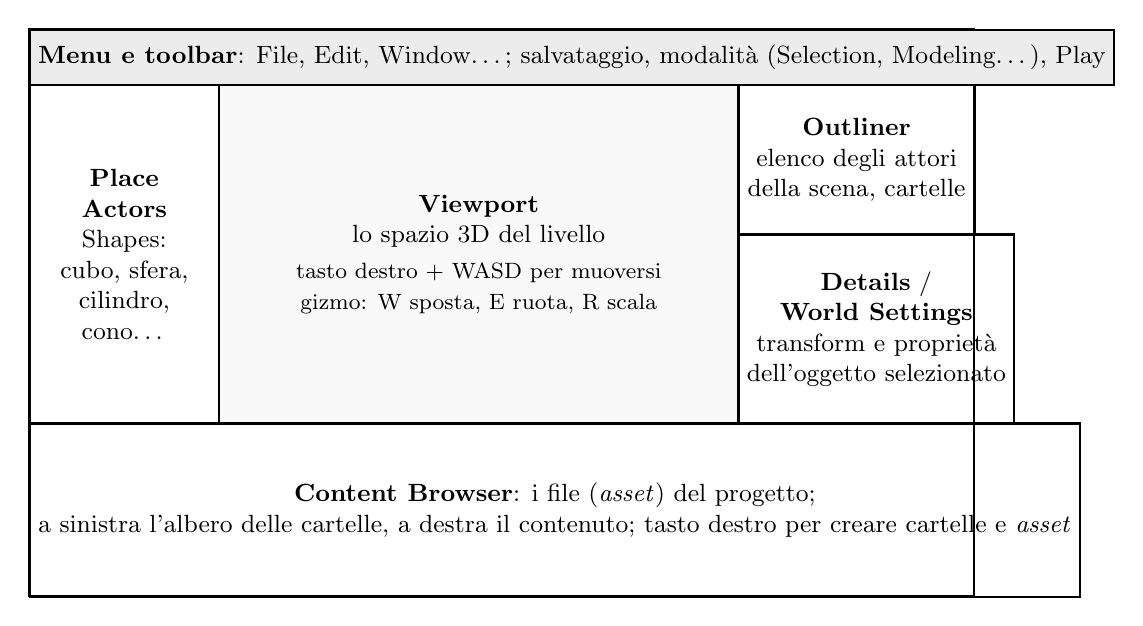
\begin{tikzpicture}[
  font=\small,
  ue1pan/.style={draw, thick, align=center, inner sep=3pt},
  ue1note/.style={font=\footnotesize, align=left, text width=3.4cm}
]
  % cornice
  \draw[thick] (0,0) rectangle (12,7.2);
  % toolbar
  \node[ue1pan, minimum width=12cm, minimum height=0.7cm, anchor=north west, fill=gray!15]
    at (0,7.2) {\textbf{Menu e toolbar}: File, Edit, Window\ldots; salvataggio, modalità
    (Selection, Modeling\ldots), Play};
  % place actors
  \node[ue1pan, minimum width=2.4cm, minimum height=4.3cm, anchor=north west]
    at (0,6.5) {\textbf{Place}\\\textbf{Actors}\\Shapes:\\cubo, sfera,\\cilindro,\\cono\ldots};
  % viewport
  \node[ue1pan, minimum width=6.6cm, minimum height=4.3cm, anchor=north west, fill=gray!5]
    at (2.4,6.5) {\textbf{Viewport}\\lo spazio 3D del livello\\[2pt]
    \footnotesize tasto destro + WASD per muoversi\\\footnotesize gizmo:
    W sposta, E ruota, R scala};
  % outliner
  \node[ue1pan, minimum width=3cm, minimum height=1.9cm, anchor=north west]
    at (9,6.5) {\textbf{Outliner}\\elenco degli attori\\della scena, cartelle};
  % details
  \node[ue1pan, minimum width=3cm, minimum height=2.4cm, anchor=north west]
    at (9,4.6) {\textbf{Details} /\\\textbf{World Settings}\\transform e proprietà\\
    dell'oggetto selezionato};
  % content browser
  \node[ue1pan, minimum width=12cm, minimum height=2.2cm, anchor=north west]
    at (0,2.2) {\textbf{Content Browser}: i file (\emph{asset}) del progetto;\\
    a sinistra l'albero delle cartelle, a destra il contenuto; tasto destro per creare
    cartelle e \emph{asset}};
\end{tikzpicture}
\caption{Una disposizione tipica dell'editor, come quella mostrata da Igor. Ogni pannello
si può spostare, agganciare ad altri o chiudere; il menu Window li riapre.}
\label{ue1:fig:editor}
\end{figure}

\paragraph{Le cartelle, e i loro colori.} Nel Content Browser, con il \textbf{tasto
destro}, si possono creare vari tipi di \emph{asset}; per cominciare, una cartella:
\textbf{New Folder}, chiamata ``prova''. Si possono creare tutte le cartelle che si
vogliono, ``in modo da avere ordine''. Una ``piccola chicchetta'': con il tasto destro
su una cartella, \textbf{Set Color}, la si può \textbf{colorare} (Igor la fa blu), un
feedback visivo che rende la navigazione molto più veloce. Il Content Browser mostra le
cartelle in due modi: a destra come in un \emph{explorer}, a sinistra come un albero ``a
cascata''. Se si mette una cartella dentro un'altra, a sinistra compare una piccola
freccia che apre la cartella sottostante: cartelle e sottocartelle.

\paragraph{L'ordine, per sé e per gli altri.} ``È molto importante l'organizzazione.'' Le
cartelle si riempiranno di \emph{asset}, e bisognerà cercarne uno solo senza sapere dove
andare. L'ordine serve ``non solo per la salvezza vostra, ma anche dei vostri possibili
collaboratori'': ``vi assicuro che quando siete ordinati, la gente vi ringrazia''.

\paragraph{Approfondimento: il Content Drawer e la definizione di \emph{asset}.} Nella
disposizione predefinita di Unreal Engine 5 il Content Browser non è sempre aperto: lo si
richiama dal pulsante \textbf{Content Drawer} in basso a sinistra (o con
Ctrl+Spazio), e lo si può agganciare stabilmente all'interfaccia (``Dock in Layout''),
come ha fatto Igor. Romero e Sewell definiscono l'\emph{asset} come ``un pezzo di
contenuto di un progetto Unreal'': materiali, \emph{static mesh} e Blueprint sono tutti
\emph{asset}. Quando si trascina un \emph{asset} dal Content Browser nel livello,
l'editor ne crea una \textbf{copia} da piazzare nella scena: l'\emph{asset} resta uno, le
sue istanze nel livello possono essere molte. Gli stessi autori descrivono l'Outliner
come l'elenco degli oggetti presenti nel livello, e i Details come il pannello che
mostra le proprietà modificabili dell'oggetto selezionato.

% ---------------------------------------------------------------------
\section{Il primo cubo e il \emph{transform}}
\label{ue1:sec:transform}

\paragraph{Place Actors.} Gli \emph{actor} sono gli elementi di gioco. Dal pannello
\textbf{Place Actors} (se manca: Window, Place Actors), nella sezione \textbf{Shapes},
si prende un \textbf{cubo} e lo si trascina nella viewport. ``Ecco a voi un cubetto
renderizzato'': il primo cubo in Unreal, ``e ne avrete tanti''.

\paragraph{I tre assi.} Sul cubo compaiono tre frecce: sono i tre assi principali,
\textbf{X}, \textbf{Y} e \textbf{Z}, lungo i quali lo si può muovere. Ogni asse ha il
suo colore: \textbf{X rosso}, \textbf{Y verde}, \textbf{Z blu}.

\paragraph{Il \emph{transform}.} Di ogni oggetto si possono modificare
\textbf{locazione}, \textbf{rotazione} e \textbf{scala}. L'insieme dei tre è il
\textbf{\emph{transform}} (``quando parleremo di \emph{transform}, ricordatevelo''), e
lo si rivedrà ``a oltranza''. Lo si modifica in due modi: con le frecce nella viewport,
o con i numeri nel pannello \textbf{Details}.

\paragraph{I numeri nei Details.} Nei Details la locazione del cubo è, per esempio, 480,
430, 120: è la \textbf{raffigurazione numerica}, in unità di Unreal, del punto in cui si
trova l'oggetto. Se si scrive 0 al posto del primo valore e si preme Invio, ``poplà'':
la coordinata X del cubo adesso è 0. Se si trascina una freccia guardando i numeri, si
vede il valore crescere o diminuire, andare in positivo o in negativo: è il verso
dell'asse.

\paragraph{Unreal ragiona in centimetri.} ``Molto importante'': \textbf{l'unità di Unreal
è il centimetro}. Se un oggetto va spostato di tre metri, lo si sposta di 300 unità.
Nella griglia del pavimento ogni riquadro, dice Igor, è un metro, e un cubo, di
default, è un metro.

\paragraph{W, E, R.} Il \textbf{pivot} (o \emph{gizmo}) è ``questo cosettino degli
assi'', e permette tre movimenti: con \textbf{W} si sposta (locazione), con \textbf{E} si
ruota, con \textbf{R} si scala. Gli stessi tre strumenti sono anche in alto a destra
nella viewport, come icone.

\paragraph{Assi locali e assi globali.} Esistono due riferimenti: gli assi
\textbf{relativi} all'oggetto stesso (\textbf{locali}) e quelli del \textbf{mondo}
(\textbf{globali}, la sua \emph{absolute location}). Finché il cubo non è ruotato la
differenza non si vede; ma se lo si ruota fino a farlo diventare ``una specie di rombo''
e si infila nel terreno, alzarlo lungo i suoi assi locali richiede ``un doppio
movimento, così e così'', perché gli assi locali ruotano insieme a lui (``avremo il
nostro bel pivot ruotato di 40 gradi''). Con gli assi globali, invece, l'alto è sempre
l'alto. Il passaggio dall'uno all'altro si fa con l'icona in alto nella viewport:
\textbf{il cubetto con tre assi} indica il riferimento \textbf{locale}, \textbf{il
mondo} indica quello \textbf{globale}. La scelta vale per locazione e rotazione.

\paragraph{La scala è solo locale.} Non vale per la scala: \textbf{un oggetto si può
scalare solo nei suoi assi locali}. Se si scalasse un oggetto ruotato lungo gli assi del
mondo, ``verrebbe totalmente stretchato malissimo'': l'oggetto è girato in un modo e
l'asse in un altro, e allungarlo così lo deformerebbe. Unreal ``ce lo impedisce''.

\paragraph{Le unità di misura del \emph{transform}.} La locazione è in centimetri, la
\textbf{rotazione in gradi} (``io l'ho ruotato e c'è un 40''), la \textbf{scala in
unità}: 1 è la dimensione originale, 2 il doppio.

\begin{figure}[htbp]
\centering
\begin{tikzpicture}[
  font=\small,
  ue1ax/.style={-{Stealth[length=3mm]}, very thick},
  ue1box/.style={draw, thick, rounded corners=3pt, text width=3.6cm, align=left,
               inner sep=5pt}
]
  % assi
  \coordinate (o) at (0,0);
  \draw[ue1ax, red!75!black] (o) -- (2.2,0) node[right]{X};
  \draw[ue1ax, green!50!black] (o) -- (1.2,1.1) node[above right]{Y};
  \draw[ue1ax, blue!75!black] (o) -- (0,2.2) node[above]{Z};
  \fill (o) circle (2pt);
  \node[below=0.2cm of o, font=\footnotesize, align=center]
    {pivot: X rosso, Y verde, Z blu};
  % riquadri
  \node[ue1box, right=2.8cm of o, yshift=1.6cm] (loc)
    {\textbf{Location} (\textbf{W})\\in centimetri\\locale o globale};
  \node[ue1box, below=0.25cm of loc] (rot)
    {\textbf{Rotation} (\textbf{E})\\in gradi\\locale o globale};
  \node[ue1box, below=0.25cm of rot] (sca)
    {\textbf{Scale} (\textbf{R})\\in unità (1 = originale)\\solo locale};
  \node[draw, thick, dashed, fit=(loc)(rot)(sca), inner sep=6pt,
    label={[font=\small\bfseries]above:Transform}] {};
\end{tikzpicture}
\caption{Gli assi e il \emph{transform}. Lo \emph{snapping} (sezione
\ref{ue1:sec:snap}) si imposta separatamente per ognuna delle tre componenti.}
\label{ue1:fig:transform}
\end{figure}

\paragraph{Il tasto Fine.} Un'altra ``piccola chicchetta'': se si piazza un cubo in
aria e si preme il tasto \textbf{Fine} (\emph{End}, quello ``sopra le frecce''), il cubo
cade sulla prima superficie che trova sotto di sé. ``Molto utile'', perché evita di
stare lì ad abbassarlo a occhio.

\paragraph{I Details seguono la selezione.} Ogni volta che si clicca un oggetto, i Details
mostrano \emph{quell'}oggetto: due cubi hanno due locazioni, due rotazioni, due scale.
\textbf{Per modificare i parametri di un oggetto, bisogna selezionarlo.}

\paragraph{Lavorare con i numeri.} I numeri dei Details sono lo strumento preciso, e
sono molto usati, per esempio, dai level designer: ``dobbiamo allargare il corridoio di
tre metri''. Igor allunga un cubo di tre metri sull'asse Y. Nei campi numerici si può
anche scrivere, oppure \textbf{trascinare}: si mette il mouse sul campo e lo si fa
scorrere a destra e a sinistra (``slidando'') per cambiare il valore, su qualunque asse,
per locazione, rotazione e scala.

\paragraph{Reset.} Accanto a ogni gruppo di valori c'è una \textbf{freccetta}: cliccandola,
il valore torna a quello originale (la scala torna a 1, la locazione al punto di
partenza).

% ---------------------------------------------------------------------
\section{Muoversi, duplicare, raggruppare}
\label{ue1:sec:navigazione}

\paragraph{Forme e pivot.} Si possono piazzare tanti \emph{actor} diversi: cilindri,
coni, sfere. Il pivot è al \textbf{centro} di ogni figura, e per questo un cilindro,
appena piazzato, è ``mezzo interrato''. Per \textbf{scalare su tutti gli assi
insieme} si prende il centro del gizmo di scala e si trascina verso l'esterno (allarga)
o verso l'interno (stringe); trascinando una sola maniglia si scala su un solo asse.

\paragraph{Duplicare con Alt.} Igor costruisce un tavolino con un cilindro schiacciato e
uno allungato. Serve un altro pezzo uguale: bisogna prendere un altro cilindro e rifare
tutto? No: \textbf{si tiene premuto Alt e si trascina} (o si ruota) l'oggetto, e se ne
crea una copia esatta. ``Lo userete a manetta.'' Funzionano anche \textbf{Ctrl+C} e
\textbf{Ctrl+V}. Una studentessa, abituata a Blender, si confonde: premeva Alt e lo
lasciava. Alt va \textbf{tenuto premuto mentre si trascina}, ``non è solo \emph{tap}
Alt''.

\paragraph{Muoversi nella viewport.} ``Mi sono dimenticato di dirvelo, perdonatemi'':
per muoversi nella viewport si tiene premuto il \textbf{tasto destro} del mouse e si
usano \textbf{W, A, S, D}, come in un gioco in prima persona; muovendo il mouse si
ruota la camera. Uno studente scopre da solo che \textbf{E} sale e \textbf{Q} scende:
``bravissimo, esatto''. Bisogna cliccare dentro la viewport: è la camera dell'editor,
non quella del gioco.

\paragraph{Seguire un oggetto.} Se si tiene premuto \textbf{Shift} mentre si trascina un
oggetto, la camera lo \textbf{segue} nel movimento: utile per piazzamenti
particolari.

\paragraph{Selezionare più oggetti.} Per selezionare più oggetti si tiene premuto
\textbf{Shift} (o Ctrl) e si cliccano uno dopo l'altro. Con il palo e il piano del
tavolo selezionati, Alt e trascinamento: ``pac!'', un secondo tavolino.

\paragraph{I gruppi.} Selezionare ogni volta tutti i pezzi è scomodo, perché se si
clicca il piano del tavolo si seleziona solo il piano. Si possono allora
\textbf{raggruppare}: si selezionano gli oggetti, tasto destro, \textbf{Group}, oppure
\textbf{Ctrl+G}. Intorno al gruppo compare ``una specie di reticolo verde'', e cliccando
un pezzo qualunque si seleziona il tutto. Si possono anche raggruppare dei gruppi, per
farne uno più grande. Per \textbf{sciogliere} un gruppo: \textbf{Shift+G}, oppure tasto
destro, Groups, \textbf{Ungroup}.

\paragraph{Ctrl+Z.} ``Qua funziona'': \textbf{Ctrl+Z} annulla. ``Sappiatelo, ogni
errore può essere cancellato, o almeno per poco.''

\paragraph{I gruppi non sono un oggetto unico.} Igor fa vedere un limite: se si
\textbf{scala} un gruppo, Unreal non lo scala come un oggetto unico; ogni pezzo si
scala rispettando i propri assi relativi. Per avere un oggetto davvero unico bisognerà
creare una \textbf{static mesh}, ``che vedremo in seguito''.

\paragraph{Mesh e static mesh.} Una \textbf{mesh} è un oggetto solido formato da
poligoni: quando qualcuno dice ``mi serve la mesh del tavolo'' intende il
\textbf{modello 3D} del tavolo. La \textbf{static mesh} è un tipo di mesh; esistono anche
le \textbf{dynamic mesh}, ``un discorso che vedremo più avanti''.

\paragraph{Approfondimento: \emph{transform} relativi nei Blueprint.} Il comportamento dei
gruppi anticipa un tema che nei Blueprint tornerà spesso. Romero e Sewell, nel capitolo
sui nodi matematici, distinguono il \textbf{\emph{transform} del mondo} di un attore
(la sua posizione assoluta nel livello) dal \textbf{\emph{transform} relativo} dei suoi
componenti, che è relativo al componente ``genitore''. Il loro esempio è un tavolo con
sopra una statua: se si sposta il tavolo, la statua lo segue; se si cambia il
\emph{transform} relativo della statua, il tavolo resta dov'è. È il modo in cui, dentro
una Blueprint Class, si costruiscono oggetti composti che si muovono come un tutt'uno.

% ---------------------------------------------------------------------
\section{Lo \emph{snapping} e la velocità della camera}
\label{ue1:sec:snap}

\paragraph{Lo \emph{snapping}.} Ruotando un oggetto, l'editor mostra un numero che sale
a scatti: 20, 30, 40, 50, 60, 70 gradi. È lo \textbf{\emph{snap}}, che si controlla in
alto a destra nella viewport: ci sono tre pulsanti, per locazione, rotazione e scala,
ognuno con un valore. \textbf{Se il pulsante è azzurro, lo \emph{snap} è attivo.}
\begin{itemize}
  \item Senza \emph{snap} di rotazione l'oggetto ruota liberamente, con i decimali; con
        lo \emph{snap} a 10, ruota di dieci gradi alla volta. Cliccando sul numero si
        sceglie il passo: 5, 10, 15, 30, 45, 60, 90, 120 gradi. Con 120, ``pam!'',
        diretto da 0 a 120; con 5, una rotazione più fine.
  \item Lo stesso vale per la \textbf{locazione}: con lo \emph{snap} l'oggetto si muove
        ``a scattini'' (di 1, 5, 10, 50 unità\ldots), senza si muove di qualunque
        valore, decimali compresi.
  \item E per la \textbf{scala}: senza \emph{snap} si scala ``quanto mi pare'', con lo
        \emph{snap} a passi anche molto piccoli, come 0,25.
\end{itemize}
Se lo \emph{snapping} impedisce di mettere un pezzo dove si vuole, ``basta
disattivarlo''.

\paragraph{La velocità della camera.} Per raggiungere ``quella montagna là'' si può
\textbf{velocizzare la camera}: mentre ci si muove (tasto destro premuto), si gira la
\textbf{rotellina del mouse} in avanti per andare più veloci e indietro per andare più
lenti, quando bisogna osservare un oggetto da vicino con precisione (Igor scende fino a
una velocità di 0,03 per guardare sotto il tavolino).

% ---------------------------------------------------------------------
\section{L'Outliner e l'ordine della scena}
\label{ue1:sec:outliner}

\paragraph{L'elenco della scena.} L'\textbf{Outliner} (se manca: Window, Outliner) è una
raffigurazione a lista di \textbf{tutti gli oggetti in scena}. Se si duplica un cono,
nell'Outliner compaiono Cone, Cone2, Cone3, Cone4\ldots{} Un oggetto si può selezionare
sia nella viewport sia nell'Outliner, ed è utile quando ``avete un bel \emph{pack} di
roba'' da gestire. Per eliminare un oggetto: \textbf{Canc} (\emph{Delete}).

\paragraph{Le cartelle dell'Outliner.} Anche nell'Outliner si possono creare cartelle, e
a Igor ``aiuta molto'' nella pianificazione e nel piazzamento. Tasto destro
nell'Outliner, \textbf{Create Folder}, e si crea una cartella ``Coni''. Poi si
selezionano i coni: visto che sono elencati per nome, si clicca il primo, si tiene
premuto \textbf{Shift} e si clicca l'ultimo, e si seleziona tutta la lista; si
trascinano dentro la cartella. Da quel momento, invece di cliccarli uno per uno, basta
il tasto destro sulla cartella e \textbf{Select All Descendants}: ``eccoli qua''.

\paragraph{Perché farlo subito.} ``Immaginatevi una scena intera, gigantesca.'' Senza
ordine si passano ``tre quarti d'ora'' a cliccare un oggetto dopo l'altro; con le
cartelle, un tasto e si è fatto. ``Vi risparmiate molto tempo.''

\paragraph{Il tasto G.} Un ultimo tasto, che Igor spiega durante la dimostrazione: se il
pivot ``scompare'', bisogna premere \textbf{G}. G passa dalla visualizzazione
dell'editor, con gli aiuti visivi, a quella ``normale'' del mondo di gioco, in cui gli
aiuti sono nascosti.

\paragraph{Approfondimento: la Game View.} Il comando si chiama \textbf{Game View}: con G
la viewport mostra la scena come la vedrebbe il giocatore, nascondendo icone,
\emph{gizmo} e oggetti che nel gioco sono invisibili (le icone delle luci, i volumi, i
punti di partenza del giocatore). È comodo per giudicare l'aspetto finale di una scena;
ma se lo si attiva per sbaglio sembra che gli strumenti siano spariti, ed è per questo
che Igor lo nomina proprio quando il pivot ``scompare''.

\begin{table}[htbp]
\centering
\small
\begin{tabular}{@{}p{4.3cm}p{8.7cm}@{}}
\toprule
\textbf{Comando} & \textbf{Che cosa fa} \\
\midrule
Tasto destro + W A S D & muoversi nella viewport; con il mouse si ruota la camera \\
Tasto destro + E / Q & salire / scendere \\
Rotellina (durante il movimento) & velocità della camera: avanti più veloce, indietro
  più lenta \\
W / E / R & gizmo di locazione / rotazione / scala \\
Icona cubetto / mondo & assi locali / globali (per locazione e rotazione) \\
Pulsanti azzurri dello \emph{snap} & attivano lo \emph{snapping} e ne scelgono il
  passo \\
Fine (\emph{End}) & fa cadere l'oggetto sulla superficie sottostante \\
Alt + trascinamento & duplica l'oggetto (Alt tenuto premuto) \\
Ctrl+C / Ctrl+V & copia e incolla \\
Shift + clic & selezione multipla; nell'Outliner, selezione di un intervallo \\
Shift + trascinamento & la camera segue l'oggetto \\
Ctrl+G / Shift+G & raggruppa / separa (anche: tasto destro, Groups) \\
Ctrl+Z & annulla \\
Canc (\emph{Delete}) & elimina l'oggetto selezionato \\
G & Game View: mostra o nasconde gli aiuti dell'editor \\
Freccetta accanto ai valori & riporta il valore all'originale \\
Ctrl+S & salva \\
\bottomrule
\end{tabular}
\caption{I comandi della prima lezione. Tutti valgono nel Level Editor di Unreal Engine
5.5 con le impostazioni predefinite.}
\label{ue1:tab:comandi}
\end{table}

% ---------------------------------------------------------------------
\section{Esercitazione: il ristorante dei tre tavoli}
\label{ue1:sec:esercitazione}

Con quello che si è imparato, ``una piccola esercitazione''. Bisogna costruire, con le
forme di base, \textbf{tre tavoli con le loro sedie}:
\begin{enumerate}
  \item un tavolo con \textbf{tre posti}: ``vengono tre ospiti a cena'';
  \item un \textbf{tavolo quadrato} per \textbf{cinque ospiti};
  \item una \textbf{cena romantica}: un tavolo per \textbf{due}, ``e se volete
        metteteci pure la candela''.
\end{enumerate}
Non serve una sedia precisa: ``l'importante è che applicate tutto quello che abbiamo
fatto''. Chi non riesce oggi può farlo per la volta successiva (``assolutamente''), e
riguardare la registrazione.

\paragraph{Partire da una reference.} Un consiglio, ``soprattutto per voi artisti'': per
fare qualcosa di artistico, prendere una \textbf{reference}. Ma non una sedia troppo
complessa: ``non ci interessa fare una cosa bella e bellissima''. Igor sceglie una
sedia ``molto semplice'', la ``sedia della nonna che vi fa il ragù''.

\paragraph{La dimostrazione.} Igor costruisce la sua sedia passo per passo, ed è un buon
riassunto di tutta la seconda parte:
\begin{enumerate}
  \item un cubo, scalato con lo \emph{snap} a 0,25, per la seduta; la freccetta di reset
        per riportarlo alle dimensioni di partenza quando serve (``le sedie sono alte
        più o meno un metro'');
  \item la prima gamba, posizionata (``se avete problemi con lo \emph{snapping}, basta
        disattivarlo'');
  \item le altre gambe: Shift per selezionare, Alt per duplicare. Ne viene ``questo
        bellissimo sgabello'', con le gambe ``non proprio precisissime'';
  \item lo schienale, duplicando altri pezzi per il dorso;
  \item tutti i pezzi selezionati e \textbf{Ctrl+G}, ``perché sennò dobbiamo fare ogni
        volta uno, due, tre, quattro'';
  \item la sedia accostata al tavolo (``è un po' spesso questo tavolo, ci saranno delle
        ginocchiate incredibili, ma non ci importa'').
\end{enumerate}

\paragraph{Si può allineare un oggetto a un altro?} Uno studente, che oggi può solo
guardare, chiede se c'è un modo di allineare le gambe della sedia a un oggetto, visto
che a mano non è semplice. Igor risponde che non è una cosa che in Unreal si fa
``professionalmente'': strumenti di allineamento precisi ci sono nei programmi di
modellazione, come Blender e Maya. In Unreal ci sono il tasto \textbf{Fine}, lo
\emph{snapping}, il lavoro ``un po' a mano'', i \emph{plugin}, oppure la
\textbf{Modeling Mode}, la modalità di modellazione dell'editor, con strumenti più
precisi, che si vedrà in seguito.

\paragraph{Gli strumenti si somigliano.} Lo stesso studente nota che, in attesa del
download, ha usato \textbf{Inkarnate}, un programma per disegnare mappe, e che i
principi visti finora sono ``molto simili''. ``Sì, assolutamente'': sono principi
condivisi dai vari game engine e dai programmi grafici. In Unity ``magari qualche
bottone è un po' diverso'', ma le funzioni sono simili; ``si impara a muoversi da una
parte e si impara a muoversi dall'altra''. Igor mostra anche \textbf{Dungeon
Scrawl}\footnote{Igor ci arriva per tentativi: ``Dungeon Crawler'', ``Dungeon
Designer'', ``Dungeon Scroll''.}, uno strumento per disegnare mappe per le partite di
D\&D con gli amici, usato anche per il level design.

\paragraph{I risultati.} Dopo una ventina di minuti di lavoro individuale, i
``ristoratori in erba'' mostrano i loro tavoli.
\begin{itemize}
  \item Uno studente ha aggiunto una \textbf{luce} per la candela, ma la candela fa
        ombra. Igor gli mostra come risolvere: si seleziona la luce e nei Details, in
        basso, si toglie la spunta a \textbf{Cast Shadows}.
  \item Qualcuno ha fatto un tavolo rettangolare invece che quadrato: ``va benissimo,
        tranquilli''.
  \item Uno studente, che ha appena finito il download, ha fatto solo la base del tavolo
        e una gamba della sedia, sottilissima. Igor ricorda che Unreal lavora in
        centimetri, e quella gamba è di pochi centimetri: ``non ci farei sedere
        nessuno, potrebbe crollare''. Ma ``è soggettivo''.
\end{itemize}
``A parte l'ironia'', la conclusione è che gli oggetti in sé contano poco: conta capire
come ci si muove in Unreal, duplicando, scalando, muovendo, ruotando. ``Questa è la cosa
più importante che oggi impariamo.''

\paragraph{Una cartella per ogni tavolo.} Un'ultima richiesta: mettere ogni gruppo in una
cartella dell'Outliner. Create Folder, ``Tavolo da due'', si selezionano i pezzi e li si
trascina dentro; poi ``Tavolo da tre'', e così via. Con Select All Descendants si
riprende il tavolo intero in un clic.

% ---------------------------------------------------------------------
\section{Salvare la mappa, e la chiusura}
\label{ue1:sec:chiusura}

\paragraph{Salvare.} Per salvare il lavoro c'è il classico \textbf{Ctrl+S}. Siccome la
mappa è stata creata ``da nulla'', la prima volta Unreal chiede dove salvarla: le si dà
un nome (``MappaProva'') e la si salva dentro la cartella ``prova'' del Content
Browser. In basso a destra, poi, l'editor tiene il conto delle modifiche non salvate:
se si sposta anche solo una sedia, compare l'indicazione degli oggetti
\textbf{\emph{unsaved}}, ``tutti gli oggetti che devo salvare''.

\paragraph{Che cos'è il secondo file?} Uno studente nota che il salvataggio crea anche un
secondo file, un \textbf{HLOD Layer}\footnote{Nella trascrizione ``Halodle'' e ``Halod
Layer''.}. Igor spiega che dipende dalla mappa: quella su cui hanno lavorato contiene un
\textbf{landscape}, le montagne che si vedono in fondo. Il landscape è un piano che si
può modellare con uno strumento apposito per formare, per esempio, il paesaggio di
sfondo; il file salva come quel piano è composto. La volta successiva si userà una
mappa davvero vuota, senza landscape.

\paragraph{Approfondimento: LOD e HLOD.} \textbf{LOD} sta per \emph{level of detail}:
lo stesso oggetto esiste in più versioni, con un numero decrescente di poligoni, e
l'engine usa quelle più semplici quando l'oggetto è lontano dalla camera, dove i
dettagli non si vedrebbero comunque. È la risposta pratica al compromesso della
sezione~\ref{ue1:sec:rendering} tra precisione e peso. Gli \textbf{HLOD}
(\emph{hierarchical} LOD) fanno lo stesso a livello di gruppi: interi blocchi lontani
della mappa vengono sostituiti da un'unica versione semplificata. Le mappe ``a mondo
aperto'' di Unreal Engine 5, con il landscape, li usano per impostazione predefinita, ed
è per questo che il salvataggio crea un file di \emph{HLOD Layer}.

\paragraph{Le ultime domande.} Come si separano gli oggetti raggruppati? ``Shift+G, oppure
tasto destro, Ungroup: se lo cerchi c'è proprio scritto.'' Quando arriva la
registrazione? Sul sito, ``credo il giorno dopo''. Le foto dei lavori si possono mandare
a Igor su Discord, ``tranquillamente'' (``quando ci sono, vi rispondo''), anzi in un
\emph{thread} o un canale apposito, ``così almeno è più ordinato e non mi riempite la
casella privata''.

\paragraph{Il calendario.} Giovedì si rivede Igor; il martedì successivo c'è Davide, con
la parte artistica; poi le lezioni si alternano, ``settimana a settimana''. Sono le 19:
``per chi tra poco cena, auguro buona cena a tutti''. ``Se avete domande, fatele adesso o
tacete fino alla prossima volta.'' ``Ciao, ragazzi.''

% ---------------------------------------------------------------------
\section*{Punti chiave del capitolo}
\addcontentsline{toc}{section}{Punti chiave del capitolo}

\begin{itemize}
  \item Il \textbf{game engine} è ``il calderone'' che riunisce 3D art, programmazione e
        design in un unico ambiente, con fisica e collisioni, suono, animazione,
        networking e IA. Lo si governa con lo \textbf{scripting}; in Unreal, con i
        \textbf{Blueprint}, un linguaggio a nodi usato anche dai programmatori (il C++
        resta per ottimizzare). Conta la \textbf{logica}, più dello strumento.
  \item Il \textbf{rendering} trasforma poligoni in pixel: \textbf{\emph{vertex
        shading}} (i vertici dei triangoli), \textbf{rasterizzazione} (quali pixel),
        \textbf{\emph{fragment shading}} (colore, luce, ombre, riflessi). Più poligoni
        = più precisione, ma più peso: ``un cubo con due milioni di poligoni'' fa
        esplodere il gioco.
  \item Il \textbf{\emph{real time rendering}} lavora tra 20 e 120 \emph{fps}: il cinema
        è a 24, il gaming a 30--60 e oltre. Un \textbf{frame} è un'immagine; la loro
        successione dà l'illusione del movimento.
  \item Unreal è il più usato perché è un \textbf{linguaggio comune}, aggiornato di
        continuo, e perché permette di \textbf{prototipare} subito: ``non ci interessa
        se è bello o brutto, è importante che funzioni'' (il prototipo di
        \emph{Expedition 33}). È usato anche nel cinema, dove conta il dettaglio più
        dell'ottimizzazione.
  \item Ciò che distingue un videogioco da un video è il \textbf{game loop}: input,
        \emph{update}, render, e di nuovo, a ogni \emph{frame}.
  \item \textbf{Ogni buona idea non esiste finché non sta su carta.} Indie, AA e AAA si
        distinguono per i soldi e per la specializzazione dei ruoli (fino ai \emph{leaf
        artist}). L'\textbf{\emph{outsourcing}} è chiedere a un altro studio una parte
        del lavoro, senza cedergli la proprietà.
  \item Tutti i ruoli toccano l'engine: \emph{blockout} e metriche per il level
        designer, momenti scriptati per il narrative designer, parametri esposti per il
        combat designer, materiali e Sequencer per gli artisti, rendering, IA e rete per
        i programmatori, Unreal Insights per il QA. \textbf{Trattate bene i vostri
        programmatori.}
  \item Un gioco è fatto di \textbf{attori, meccaniche, spazio, obiettivi, regole} (e a
        volte \textbf{tempo}); il divertimento è una \textbf{conseguenza}, e il gameplay
        nasce dalle \textbf{scelte}. Meccanica = che cosa posso fare; dinamica = come lo
        faccio; estetica = come mi fa sentire. ``Un gioco per tutti non è un gioco per
        nessuno.''
  \item Il bilanciamento è un lavoro tra \textbf{designer e QA}; il feedback utile è
        quello da cui si ricava un'informazione. Far giocare chi non ha mai visto il
        gioco ``è la cosa più pura''.
  \item Per il corso serve Unreal \textbf{5.5} (la 5.5.4): l'ultimo numero è solo
        l'aggiornamento, il secondo decide la compatibilità.
  \item Le risorse: \textbf{documentazione}, forum, corsi gratuiti di
        \emph{learning}, \textbf{Fab} con i \emph{pack} gratuiti del mese (``prendeteli
        sempre''). Ma \textbf{prima la funzione, poi l'\emph{asset}}, o il progetto
        pesa 70~GB per usarne tre.
  \item Quando si preme Play gli attori vengono inizializzati e duplicati. Ogni
        movimento va reso \textbf{relativo al tempo di gioco} (\emph{delta seconds}),
        altrimenti dipende dagli \emph{fps}.
  \item Il progetto di prova: Games, \textbf{Blank}, Blueprint, Desktop, Starter
        Content, nome \textbf{senza spazi}. I template si distinguono per le
        \textbf{3C}: camera, controller, character.
  \item L'editor è fatto di \textbf{finestre} spostabili (Window le riapre): viewport,
        Details, Outliner, World Settings, \textbf{Content Browser}. Cartelle colorate
        e ordine: ``quando siete ordinati, la gente vi ringrazia''.
  \item Il \textbf{transform} è locazione (\textbf{centimetri}), rotazione
        (\textbf{gradi}) e scala (\textbf{unità}); \textbf{W, E, R}; X rosso, Y verde,
        Z blu; assi locali o globali, ma \textbf{la scala è solo locale}.
  \item \textbf{Alt + trascinamento} duplica, \textbf{Ctrl+G} raggruppa, \textbf{Fine}
        appoggia a terra, lo \textbf{\emph{snap}} azzurro fa muovere a scatti, la
        \textbf{rotellina} cambia la velocità della camera, \textbf{Select All
        Descendants} riprende un'intera cartella dell'Outliner.
\end{itemize}

%
%  Tutte le etichette di questo capitolo hanno il prefisso "ue1:"
%  (ue1:cap:..., ue1:sec:..., ue1:fig:..., ue1:tab:...), e tutti gli
%  stili TikZ hanno il prefisso "ue1" (ue1box, ue1arr, ...) per non
%  collidere con chiavi native di TikZ. Il capitolo è autonomo: non
%  contiene \ref verso altri capitoli.
%  Le figure sono ricostruzioni schematiche di quanto mostrato e detto a
%  lezione, non copie delle slide del docente. Dove la trascrizione è
%  troppo rovinata per ricostruire un dettaglio, il capitolo lo dice
%  invece di inventarlo.
% =====================================================================

\chapter[Introduzione a Unreal Engine]{Introduzione a Unreal Engine: che cos'è un
engine, chi lo usa, e il primo contatto con l'editor}
\label{ue1:cap:intro}

Questa è la \textbf{prima lezione} del corso breve di \textbf{introduzione a Unreal
Engine}, un corso che ha il suo centro nei \textbf{Blueprint}, il sistema di
programmazione visuale ``a nodi'' dell'engine di Epic Games. La lezione ha due metà
molto diverse. La prima è teorica e larga: che cos'è un \emph{software}, che cos'è un
\emph{game engine}, come un modello fatto di poligoni diventa un'immagine sullo
schermo, perché Unreal è oggi l'engine più diffuso, quali figure di una produzione lo
usano e per che cosa, e infine, con un'attività in classe, da che cosa è formato un
gioco. La seconda metà è pratica: si scarica Unreal Engine 5.5, si guardano le risorse
che Epic mette a disposizione (la documentazione, i corsi gratuiti, il negozio di
\emph{asset} Fab), si crea un primo progetto vuoto e si impara a muoversi nell'editor:
piazzare un cubo, spostarlo, ruotarlo, scalarlo, duplicarlo, raggrupparlo, ordinarlo
in cartelle. La lezione si chiude con un'esercitazione: arredare un piccolo
ristorante con tre tavoli e le loro sedie.

Il docente è \textbf{Igor}\footnote{Il docente si presenta come ``Igor Ripanti''; il
cognome è quello della trascrizione automatica, che altrove storpia quasi tutti i nomi
propri, e il capitolo non è in grado di verificarlo.}, che si presenta come ex alunno
della stessa scuola degli studenti, ``precisamente per quanto riguarda game
design''\footnote{La trascrizione dice ``sono stato un alunno di Live'': il nome della
scuola è con ogni probabilità storpiato.}. Ha lavorato a \textbf{\emph{Steel Seed}},
``principalmente come \emph{level designer}''; ma ``essendo un ambiente indie'' faceva
``un po' di tutto'', anche programmazione e \emph{scripting}, e quindi ha fatto ``uso
intensivo'' di Unreal Engine ``e di tutte le sue feature''. Il corso è diviso tra due
docenti: con Igor la parte di programmazione e di ``piccole feature''; con
\textbf{Davide}, a partire dal 26 del mese, una parte ``un po' più artistica''. Le
lezioni si alternano: il giovedì successivo gli studenti saranno di nuovo con Igor, il
martedì dopo con Davide.

La lezione è \textbf{online}, su Zoom, con un server Discord del corso per i
materiali e le domande; inizia poco dopo le 17 e finisce alle 19, con una pausa di una
decina di minuti verso le 17 e mezza\footnote{Igor, credendo per errore che la lezione
finisse alle 18 (``sono da un altro corso che finiva alle 18''), dopo la pausa annuncia
che ``manca mezz'ora alla fine''; gli studenti lo correggono (``nella mail c'era
scritto'' alle 19), e il docente ha ``un'altra ora'' per la parte pratica.}. Gli
studenti sono tutti \textbf{nuovi iscritti al primo anno}, di corsi diversi: game
design (la maggioranza), narrative design, character animation, 3D art e
programmazione. Il corso breve, in altre parole, è comune a figure che in una
produzione useranno Unreal in modi molto diversi, ed è proprio da questa varietà che
Igor parte.

Tre avvertenze di lettura. La prima: la trascrizione è automatica e storpia moltissimi
nomi. Unreal diventa ``Arreal'', ``Arial Engine'', ``ArrayLange'', ``ArrayLab'',
``Arrival Engine'', ``Arrial'', ``Ariane Engine'', ``Riala'' e ``a Real Engine'';
\emph{Clair Obscur: Expedition 33} è ``Expedition'' e ``Spedisce 33''; Sandfall
Interactive è ``Send Follow Interactive''; \emph{shader} è anche ``scender''. Dove la
ricostruzione è sicura il capitolo usa la forma corretta e, la prima volta, lo segnala
in nota; dove non lo è riporta la forma della trascrizione e lo dice. La seconda: in
più punti la registrazione contiene lunghi blocchi di testo senza senso e ripetuto
(``qual è la risposta che ci può essere?'', ``a parte il plus time\ldots''): sono
artefatti del riconoscimento vocale durante la pausa e i momenti di lavoro
individuale, e il capitolo li ignora. La terza: la seconda metà della lezione è una
dimostrazione dal vivo nell'editor; il capitolo ricostruisce i passaggi da ciò che Igor
dice mentre li fa, e li completa, dove serve, con i nomi esatti dei comandi.

\paragraph{Come leggere questo capitolo.} Il capitolo segue l'ordine della lezione.
Le figure ricostruiscono gli schemi spiegati a voce o sulle slide (la pipeline di
rendering, il \emph{game loop}, gli elementi di un gioco, l'interfaccia dell'editor,
il \emph{transform}); le tabelle riassumono i ruoli della produzione e le scorciatoie
da tastiera della seconda parte. Qua e là, dei paragrafi di \textbf{approfondimento}
collegano la lezione al libro \emph{Blueprints Visual Scripting for Unreal Engine 5}
di Marcos Romero e Brenden Sewell, che sarà il testo di riferimento per questa parte
del libro, e a qualche nozione tecnica generale; sono segnalati come tali e non fanno
parte della lezione.

Il percorso del capitolo:
\begin{enumerate}
  \item le presentazioni e le esperienze degli studenti (sezione
        \ref{ue1:sec:presentazioni});
  \item il \textbf{software}, il \textbf{game engine} e lo \textbf{scripting}, con i
        Blueprint (sezione \ref{ue1:sec:engine});
  \item il \textbf{rendering 3D}: poligoni, \emph{vertex shading}, rasterizzazione,
        \emph{fragment shading}; poi il \emph{real time rendering} e i \emph{frame}
        (sezioni \ref{ue1:sec:rendering} e~\ref{ue1:sec:realtime});
  \item \textbf{Unreal Engine}: perché è così usato, la prototipazione, i giochi, gli
        engine di una volta, il cinema, il \textbf{game loop} (sezioni
        da~\ref{ue1:sec:unreal} a~\ref{ue1:sec:gameloop});
  \item la \textbf{produzione} e i \textbf{ruoli} che toccano l'engine (sezioni
        \ref{ue1:sec:produzione} e~\ref{ue1:sec:ruoli});
  \item l'attività in classe: \textbf{da che cosa è formato un gioco}, e le domande
        prima della pausa (sezioni \ref{ue1:sec:elementi} e~\ref{ue1:sec:domande});
  \item il \textbf{download} della 5.5, le \textbf{risorse} (documentazione,
        \emph{learning}, Fab) e un po' di teoria sul \emph{Play in Editor} e sul
        \emph{delta time} (sezioni da~\ref{ue1:sec:download} a~\ref{ue1:sec:pie});
  \item il primo contatto con l'\textbf{editor}: il progetto, l'interfaccia, il
        \textbf{transform}, la navigazione, l'organizzazione (sezioni
        da~\ref{ue1:sec:progetto} a~\ref{ue1:sec:outliner});
  \item l'\textbf{esercitazione dei tre tavoli}, il salvataggio e la chiusura (sezioni
        \ref{ue1:sec:esercitazione} e~\ref{ue1:sec:chiusura}).
\end{enumerate}

% ---------------------------------------------------------------------
\section{Presentazioni: chi c'è, e chi ha già aperto un engine}
\label{ue1:sec:presentazioni}

La lezione comincia con qualche minuto di attesa (``aspettiamo cinque, dieci minuti''),
un appello e una richiesta: accendere la webcam, ``così almeno ci vediamo un po' in
faccia''. A chi non ha una webcam Igor suggerisce le applicazioni che trasformano il
telefono in una webcam, ``come se ti facessi una videochiamata'': lui usa di solito
\emph{Iriun}\footnote{Nella trascrizione ``Ingur'' e ``Iruin''; si tratta con ogni
probabilità di \emph{Iriun Webcam}, un'applicazione gratuita che fa esattamente
questo.}. I lavori in corso nell'edificio del docente producono ``rumori molesti'' per
tutta la lezione, e Igor se ne scusa.

Poi il giro di presentazioni: nome, corso, ``un piccolo background''. Tutti sono iscritti
al primo anno; i corsi sono game design, character animation, narrative design (più di
uno), 3D art e programmazione. ``C'è una bella quantità di nuovi compagni di design'',
commenta Igor, ``quindi avremo pane per i nostri denti'', oltre ovviamente a 3D art e
programmazione.

\paragraph{Chi ha già usato un engine?} La domanda successiva è se qualcuno abbia ``mai
aperto un software di \emph{develop} per i videogiochi'': Unity, Godot, ``in
generale''. Qualcuno ha provato Godot; qualcuno un po' di Unity, seguendo un corso
online ``molto veloce'' e facendo ``un paio di giochini'', un \emph{platform} e un clone
di \emph{Flappy Bird}, ``di 3D niente''; qualcuno è ``digiuno'', e qualcun altro ha
lavorato ``con roba presa da Fab''. Igor accoglie tutte le risposte allo stesso modo:
``ci sta assolutamente''. Fab, aggiunge, sarà uno dei temi di oggi, perché è ``una
risorsa incredibile'', soprattutto per le cose gratis, quelle in sconto e i contenuti
gratuiti del mese.

\paragraph{La mentalità prima degli strumenti.} A chi parte da zero Igor dà subito una
rassicurazione che vale per tutto il corso: ``l'importante è avere la mentalità''. In
programmazione, ``molto spesso'' si tratta ``semplicemente'' di imparare a usare gli
strumenti, mentre ``la logica fa da padrone''. Passare da un engine all'altro, o da
nessun engine al primo, è soprattutto ``riabituarsi a un nuovo campo di gioco''.

% ---------------------------------------------------------------------
\section{Software, game engine e scripting}
\label{ue1:sec:engine}

\paragraph{Che cos'è un software.} Igor parte dalla definizione più semplice possibile:
il \textbf{software} è ``quello che non è hardware, fondamentalmente''. È un insieme di
istruzioni, di dati e di programmi con funzionalità precise, che ci permettono di
creare cose: strumenti di 3D art come \textbf{Blender} e \textbf{Maya}, oppure
\emph{engine} come \textbf{Unreal Engine} e \textbf{Unity}.

\paragraph{L'engine come calderone.} Il \textbf{game engine} è ``il calderone, chiamiamolo
un po' così'', che riunisce tutte le facoltà di chi sviluppa (3D art, programmazione,
design) e le mette ``in un ambiente comune'', l'ambiente di sviluppo dell'engine. Gli
engine più noti sono \textbf{Unreal}, \textbf{Unity}, \textbf{Godot} e
\textbf{GameMaker}, e ognuno contiene al suo interno molte funzionalità: i
\textbf{motori fisici}, che gestiscono le \textbf{collisioni}; la gestione dei
\textbf{suoni}; le \textbf{animazioni}; il \textbf{networking}; l'\textbf{intelligenza
artificiale} dei personaggi. Nessuna di queste cose ``si fa da sola'': ci mettono le
mani gli sviluppatori, ``tramite lo \emph{scripting}''.

\paragraph{Lo scripting, e i Blueprint.} Lo \textbf{scripting} è ``la forma di
programmazione che ci permette di entrare in interazione e creare cose all'interno
dell'engine''. Esistono molti linguaggi: Igor cita il \textbf{C}, il \textbf{C\#}
(quello di Unity) e i \textbf{Blueprint}, che sono il tipo di \emph{scripting} di Unreal
Engine e l'oggetto di questo corso. Più avanti nella lezione (sezione~\ref{ue1:sec:ruoli})
Igor tornerà sul punto: in Unreal si può programmare anche in codice (in C++), ``ma noi
non lo useremo'', perché i Blueprint bastano ``tranquillamente'', sono usati anche dai
programmatori, e ``tanti giochi nel comparto indie'' sono fatti ``solo con Blueprint,
senza mai toccare una riga di codice''. I Blueprint sono un \textbf{linguaggio a nodi}:
``prendiamo proprio e colleghiamo tutti i nodini'' per dare un senso alla
programmazione.

\paragraph{Approfondimento: le due accezioni di ``Blueprint''.} Romero e Sewell, nel
primo capitolo di \emph{Blueprints Visual Scripting for Unreal Engine 5}, fanno notare
che in Unreal la parola \emph{Blueprint} ha due significati. È il nome del
\textbf{linguaggio di scripting visuale} creato da Epic Games; ed è anche il nome di un
\textbf{tipo di oggetto di gioco} creato con quel linguaggio. I Blueprint di questo
secondo tipo sono di due specie: il \textbf{Level Blueprint}, uno per ogni livello del
gioco (non se ne possono creare altri separati), e le \textbf{Blueprint Class}, che
servono a creare oggetti interattivi riutilizzabili in qualunque livello. Un progetto di
Unreal Engine 5, aggiungono gli autori, si può sviluppare in Blueprint, in C++ o in una
combinazione dei due: si può aggiungere codice C++ a un progetto Blueprint e viceversa.
La scelta di partire dai Blueprint, quindi, non chiude nessuna porta.

% ---------------------------------------------------------------------
\section{Il rendering 3D: dai poligoni ai pixel}
\label{ue1:sec:rendering}

Un'applicazione grafica come un gioco 3D ha una particolarità: il \textbf{3D
rendering}, cioè ``la fase finale dello sviluppo di un'immagine''. È il processo che
prende un \textbf{\emph{3D asset}} (``per il linguaggio un po' più tecnico'') e ci
presenta davanti la scena vera e propria, con gli oggetti creati dai 3D artist ``che
hanno faticato tanto per poterlo fare''. Quegli oggetti sono formati da
\textbf{poligoni}.

\paragraph{Quanti poligoni ha questo oggetto?} Igor chiede se qualcuno ha mai sentito
parlare del numero di poligoni di un modello. Uno studente sì: gli sono capitati ``dei
video di ottimizzazione'' su come diminuire i poligoni ``per cercare di diminuire il
\emph{lag}''. ``Esatto, bravissimo.'' La regola è semplice, e Igor la dice con una
battuta: ``se mai doveste avere il caso fortuito di avere un cubo con due milioni di
poligoni, sappiate che il vostro gioco esploderà, probabilmente''. Nella
\textbf{viewport} (``un elemento che poi vedremo'': la finestra in cui l'engine, ma
anche Blender mentre si modella, mostra la scena) vale sempre lo stesso compromesso:
\textbf{più poligoni ci sono, più l'immagine è precisa, ma più è pesante da
renderizzare}.

\paragraph{Le tre fasi.} Il rendering di un'immagine passa per molti passaggi; ``noi oggi''
ne guardiamo tre principali (figura~\ref{ue1:fig:pipeline}).
\begin{enumerate}
  \item \textbf{\emph{Vertex shading}.} Le immagini e i modelli sono formati
        principalmente da \textbf{triangoli}, e i triangoli sono formati da
        \textbf{vertici}. I vertici definiscono la forma: in questa fase si
        identificano e si posizionano i tre punti di ogni triangolo.
  \item \textbf{Rasterizzazione.} Il triangolo così definito viene
        \emph{rasterizzato}: si stabilisce quali \textbf{pixel} dello schermo cadono
        dentro quel triangolino. Igor la spiega a partire dalla grafica 2D (``qualcuno
        ha fatto grafica?'', e una studentessa laureata in grafica conferma). Un'immagine
        \textbf{raster}, come quelle di Photoshop, è fatta di pixel; un'immagine
        \textbf{vettoriale} è fatta di vettori. La differenza: se si ingrandisce
        (``strecciate'') un'immagine raster, diventa ``sgranatissima''; un'immagine
        vettoriale la si può ingrandire ``quanto volete'' e resta uguale. Gli schermi,
        però, sono fatti di pixel: per questo i triangoli vanno rasterizzati.
  \item \textbf{\emph{Fragment shading}.} È la fase finale, quella ``vicina alla
        visualizzazione''. Ai \textbf{frammenti} (``poligoni, triangoli, chiamateli
        come vi pare'') si applicano i \textbf{colori}, la \textbf{luce}, le
        \textbf{ombreggiature} e i \textbf{riflessi}, tenendo conto della posizione
        della camera. È anche ``una parte molto artistica'', perché Unreal lavora molto
        sulla resa della luce: si possono piazzare luci, gestire come la luce entra in
        una stanza, e così via.
\end{enumerate}

\begin{figure}[htbp]
\centering
\begin{tikzpicture}[
  font=\small,
  ue1box/.style={draw, thick, rounded corners=3pt, minimum height=1.5cm,
               text width=2.6cm, align=center},
  ue1io/.style={draw, thick, dashed, rounded corners=3pt, fill=gray!10,
               minimum height=1.5cm, text width=2.0cm, align=center},
  ue1arr/.style={-{Stealth[length=3mm]}, thick}
]
  \node[ue1io] (m) {\textbf{Modello 3D}\\poligoni\\(triangoli)};
  \node[ue1box, right=0.5cm of m] (v) {\textbf{1. Vertex shading}\\i vertici
    definiscono la forma dei triangoli};
  \node[ue1box, right=0.5cm of v] (r) {\textbf{2. Rasterizzazione}\\quali pixel
    cadono dentro ogni triangolo};
  \node[ue1box, right=0.5cm of r] (f) {\textbf{3. Fragment shading}\\colore, luce,
    ombre, riflessi};
  \node[ue1io, below=0.8cm of f] (s) {\textbf{Immagine}\\sullo schermo\\(pixel)};
  \draw[ue1arr] (m) -- (v);
  \draw[ue1arr] (v) -- (r);
  \draw[ue1arr] (r) -- (f);
  \draw[ue1arr] (f) -- (s);
  \node[below=0.9cm of v, text width=6.2cm, align=left, font=\footnotesize] {Più
    poligoni $\Rightarrow$ immagine più precisa, ma più pesante da renderizzare
    (``un cubo con due milioni di poligoni'' fa esplodere il gioco).};
\end{tikzpicture}
\caption{Le tre fasi principali del rendering di cui parla Igor. Il processo reale ha
molti passaggi intermedi; la lezione si ferma a questi tre.}
\label{ue1:fig:pipeline}
\end{figure}

\paragraph{Per vertici o per frammenti.} Sulla slide, in basso a destra, ci sono due
versioni della stessa sfera illuminata. Nella prima la luce è calcolata \textbf{per
vertici}: la luce ``quasi'' lascia vedere i triangoli. Nella seconda è calcolata
\textbf{per frammenti}, cioè dopo il \emph{fragment shading}: la luce è ``molto più
diramata'', morbida, ``e fa sì che funzioni per bene''.

\paragraph{Le UV.} Igor accenna anche alle \textbf{UV}, di cui si parlerà più avanti nel
corso: sono ``delle mappe che i 3D artist creano'' e che permettono di dire come il
materiale si comporta sulla superficie del modello, come gestire e rifrangere la luce,
``questo materiale così'', e così via.

\paragraph{Approfondimento: che cosa sono le UV.} Per completezza (la lezione ci torna
solo di sfuggita): le \textbf{coordinate UV} sono il modo in cui la superficie di un
modello 3D viene ``srotolata'' su un piano a due dimensioni, come si apre la scatola di
cartone di un cubo. Le lettere U e V indicano i due assi di quel piano, per non
confonderli con gli X, Y e Z dello spazio 3D. Su quel piano si dipingono le
\emph{texture} (il colore, la rugosità, i dettagli in rilievo), che poi l'engine
``riavvolge'' sul modello durante il rendering. Un buon \emph{UV mapping} è il motivo
per cui una texture appare senza deformazioni o cuciture visibili.

% ---------------------------------------------------------------------
\section{Il \emph{real time rendering} e i \emph{frame}}
\label{ue1:sec:realtime}

In Unreal Engine il rendering è \textbf{in tempo reale}. Igor lo collega a un'esperienza
che molti studenti faranno: lo \emph{showreel}, soprattutto per chi diventerà 3D artist,
sarà ``molto accompagnato'' dal rendering di Unreal, con camere ed effetti ``fatti per
bene, scriptati'', che permettono di vedere gli oggetti ``alla massima qualità
possibile''. E come sempre: più alta è la qualità, più tempo ci vuole per renderizzare.
Il \emph{real time rendering} è il rendering che produce le immagini a una velocità
compresa, più o meno, tra i \textbf{20 e i 120 fotogrammi al secondo}.

\paragraph{Che cos'è un frame.} Un \textbf{frame} (fotogramma) è una singola immagine; la
\textbf{visualizzazione per frame} è un susseguirsi di immagini correlate l'una
all'altra che danno l'\textbf{illusione del movimento} sullo schermo. È lo stesso
principio dell'animazione: il cinema lavora a \textbf{24 \emph{frame} al secondo}
(``quando andate a vedere un film''), il gaming di solito a \textbf{30 o 60
\emph{fps}}, e c'è chi gioca a 120--144 \emph{fps} (``incredibili'', commenta Igor,
``l'\emph{fps} che se la tira tanto'').

\paragraph{Approfondimento: il budget di un frame.} Un modo utile per leggere questi
numeri è rovesciarli. A 30 \emph{fps} l'engine ha circa $1000/30 \approx 33$
millisecondi per produrre ogni immagine; a 60 \emph{fps} ne ha circa 16,7; a 120 circa
8,3. In quel tempo deve leggere gli input, aggiornare la logica di gioco (il
\emph{game loop} della sezione~\ref{ue1:sec:gameloop}) e renderizzare la scena. È per
questo che l'ottimizzazione (meno poligoni, meno luci dinamiche, nebbia più leggera)
non è un dettaglio tecnico ma una condizione per avere un gioco giocabile: tutto ciò che
non entra nel \emph{budget} fa scendere il \emph{frame rate}.

% ---------------------------------------------------------------------
\section{Unreal Engine: perché è così usato}
\label{ue1:sec:unreal}

Unreal Engine è ``il nostro bellissimo'' game engine, quello che si userà per tutto il
corso. È sviluppato da \textbf{Epic Games}, e per usarlo bisogna scaricare
l'\textbf{Epic Games Launcher} dal sito di Epic (lo si farà durante la lezione, sezione
\ref{ue1:sec:download}).

\paragraph{Il più usato.} È, dice Igor, ``proprio il più usato al momento'': ``gran parte
dei giochi moderni'', AA e AAA, tendono a usarlo. Una delle ragioni è che, essendo un
motore comune, Epic lo aggiorna continuamente, con nuove funzionalità come il
\textbf{Control Rig}, che permette per esempio di fare le animazioni in modo
procedurale. Nel launcher si vede: ogni volta propone una versione diversa da scaricare
(5.5, 5.6, 5.7\ldots), e il canale YouTube ufficiale di Unreal Engine pubblica a ogni
versione un video riassuntivo delle novità.

\paragraph{Un linguaggio comune.} La seconda ragione è che Unreal è un \textbf{linguaggio
comune}: permette ai professionisti di parlarsi e di produrre insieme. I designer, per
esempio, lo usano ``molto spesso per prototipare''. La \textbf{prototipazione} è una
fase ``molto importante'' della creazione di un gioco: ``tiro fuori l'idea dal
cappello'' e la si mette ``direttamente in engine'', usando lo \emph{scripting} per
vedere se ``questa idea che ho in testa funziona''. È ``il modo più veloce e più giusto
per capire subito se qualcosa funziona''. Poi ci sono molte altre figure che usano
l'engine nelle sue diverse caratteristiche (sezione~\ref{ue1:sec:ruoli}).

\paragraph{Alcuni giochi fatti in Unreal.} Sulla slide: \emph{A Way Out}, \emph{Ark},
\emph{Crash Bandicoot 4} (``per chi ha giocato, bellissimo'') e \emph{Fortnite}. Per
\emph{Fortnite} esiste anche una versione dell'engine, \textbf{Unreal Editor for
Fortnite} (UEFN), che permette di prendere le funzionalità del gioco e ``metterle
insieme''. Igor lo paragona a \textbf{Roblox}, che sta facendo ``un simile effetto'':
creare un \textbf{mega \emph{game template}}. Un \emph{game template} è ``il
\emph{pattern} di regole'', tutto ciò che forma il gioco, messo a disposizione delle
persone perché ci facciano ``quello che vogliono''.

\paragraph{Il caso \emph{Expedition 33}.} Igor chiede quale gioco fatto in Unreal sia
rimasto in testa agli studenti, e la risposta arriva subito: \textbf{\emph{Clair
Obscur: Expedition 33}}\footnote{Nella trascrizione quasi sempre solo ``Expedition'' o
``Expedition 33'', una volta ``Spedisce 33''.}. ``Benissimo, vedo che ci intendiamo.''
Il gioco, racconta Igor, è nato da persone che, ``per quanto dicano loro'', hanno
detto: ``non sapevamo fare un gioco, e ci siamo messi a guardare YouTube''. Igor mostra
il video del \textbf{prototipo} di \emph{Expedition 33} fatto in Unreal Engine (dopo la
solita pubblicità): è lo stadio che si affronta ``molto spesso all'inizio di una
produzione'', quello in cui ``non ci interessa se è bello o brutto, è importante che
funzioni''. Unreal permette proprio questo: mettere subito in campo le cose più usate
del gaming.

\paragraph{Le cose comuni.} Ci sono infatti tante cose ``comuni all'interno del nostro
panorama videoludico''. Il \textbf{salto}, per esempio: ``quante volte in un gioco si
salta?''. C'è chi non lo usa, ma i giochi con il salto sono ``a bizzeffe''. Unreal,
creando una sorta di \emph{template} comune, facilita molto i primi passi.

% ---------------------------------------------------------------------
\section{Gli engine di una volta, e Unreal fuori dai videogiochi}
\label{ue1:sec:storia}

\paragraph{Quando ogni gioco aveva il suo engine.} ``Non siamo lì, ragazzi, nel 2004.'' Nei
vecchi giochi, ricorda Igor, si creavano engine \textbf{apposta}: un programmatore
doveva passare dalle linee di codice alla visualizzazione in 3D, ``in tutto un processo
che andava dai due ai tre anni''. E quegli engine erano poco riutilizzabili, perché
contenevano ``\emph{pattern} di regole molto fissati''. Si trovavano comunque modi
interessanti di riusarli: Igor cita, come ``piccola curiosità'', un gioco di Shrek per
PlayStation~2 (``Shrek~2'', si corregge) realizzato modificando il motore di un gioco
del \emph{Signore degli Anelli}\footnote{L'aneddoto è riportato come lo racconta Igor,
che lo introduce con ``io mi ricordo''; il capitolo non ha verificato quale gioco del
\emph{Signore degli Anelli} e quale versione di \emph{Shrek} siano coinvolti.}.

\paragraph{Gli engine proprietari.} Esistono poi gli engine \textbf{proprietari}, come
\textbf{Source} e \textbf{Source~2} di Valve (\emph{Half-Life}): sono ``loro'', di Valve,
ma la casa mette a disposizione gratuitamente gli strumenti per creare mappe, con
l'editor \textbf{Hammer}. Unreal, invece, mette a disposizione ``tante cose diverse''
per ``mettere subito la carne sul fuoco'' e facilitare il progetto.

\paragraph{Unreal nel cinema.} Oltre ai videogiochi, Unreal è ``molto usato'' nel
\textbf{\emph{filmmaking}} e nel \emph{videomaking}. Igor mostra uno spot di
motociclette (``della Indian''): le rocce intorno al motociclista ``non esistono'', sono
renderizzate in Unreal. È ``la classica storia del \emph{green screen}'', con dietro il
lavoro di chi è esperto di Unreal. Uno studente ricorda che anche \emph{The Batman} fu
girato in parte in questo modo, e Igor conferma che ``se ne parlò'': oggi è ``molto in
voga'', perché ``nessuno ha voglia di andare di nuovo in Islanda'' per avere delle
rocce molto belle; ci si fa le rocce pre-renderizzate.

\paragraph{Ottimizzazione contro dettaglio.} I processi, però, sono ``molto
differenziati''. Nei videogiochi si parla molto di \textbf{ottimizzazione}: modelli
\textbf{\emph{low poly}}, non pesantissimi e non precisissimi, ``belli da vedere ma
ottimizzati''. Nel \emph{filmmaking} l'ottimizzazione esiste, ma conta il
\textbf{dettaglio}, perché il risultato è ``solo una raffigurazione''. Un videogioco,
invece, è \textbf{un programma in esecuzione}: continui \emph{frame}, continue
interazioni, un continuo \emph{game loop}.

\paragraph{Le rocce che si vedono ovunque.} Una battuta tra sviluppatori: esistono rocce
che ``sono le stesse, perché sono bellissime''. Sono fatte in 4K e
\textbf{scannerizzate}: qualcuno si è messo letteralmente a fotografare le rocce, le ha
digitalizzate e le ha messe gratis sull'\emph{asset store}. ``E le vedete ovunque'':
``ormai sono riconoscibili'', fatte molto bene ma molto comuni.

\paragraph{Approfondimento: \emph{virtual production} e \emph{scan}.} Le due cose di cui
parla Igor hanno un nome. La prima è la \textbf{\emph{virtual production}}: invece di
aggiungere lo sfondo in post-produzione su un \emph{green screen}, si proietta in
tempo reale l'ambiente renderizzato da Unreal su grandi pareti di LED intorno agli
attori, così che luci e riflessi siano già giusti in ripresa (la tecnica è stata resa
celebre da \emph{The Mandalorian}). La seconda è la \textbf{fotogrammetria}: si
fotografa un oggetto reale da decine o centinaia di angolazioni e un software ne
ricostruisce il modello 3D con le texture. Le rocce ``che si vedono ovunque'' vengono
quasi certamente dalla libreria \textbf{Quixel Megascans}, che Epic ha acquisito e reso
gratuita per Unreal, e che oggi è distribuita attraverso Fab.

% ---------------------------------------------------------------------
\section{Il \emph{game loop}}
\label{ue1:sec:gameloop}

Che cosa succede, allora, ``all'interno di un \emph{frame}'' di un gioco? Il
\textbf{\emph{game loop}} (figura~\ref{ue1:fig:gameloop}) è il ciclo che distingue un
videogioco da un video:
\begin{enumerate}
  \item si \textbf{inizializza} il gioco;
  \item il programma è \textbf{in attesa di un input} e lo legge: ``io premo X, A, o
        quello che è'';
  \item dopo l'input c'è un \textbf{\emph{update}}: a livello di programmazione il
        personaggio salta, si ha il movimento;
  \item si \textbf{renderizza} l'immagine;
  \item se si esce dal gioco il processo finisce; altrimenti si ricomincia dal punto 2,
        ``in questo iter continuo''.
\end{enumerate}
La differenza sostanziale tra il \emph{videomaking} e ``un vero videogioco'' è proprio
la presenza del \emph{game loop}.

\begin{figure}[htbp]
\centering
\begin{tikzpicture}[
  font=\small,
  ue1box/.style={draw, thick, rounded corners=3pt, minimum height=1.1cm,
               text width=2.6cm, align=center},
  ue1end/.style={draw, thick, rounded corners=8pt, fill=gray!15,
               minimum height=0.9cm, text width=2.0cm, align=center},
  ue1dec/.style={draw, thick, diamond, aspect=2, inner sep=1pt, text width=1.6cm,
               align=center},
  ue1arr/.style={-{Stealth[length=3mm]}, thick}
]
  \node[ue1end] (init) {Inizializzazione};
  \node[ue1box, right=0.9cm of init] (in) {\textbf{Input}\\attesa e lettura\\(premo A)};
  \node[ue1box, right=0.9cm of in] (up) {\textbf{Update}\\logica di gioco\\(il personaggio salta)};
  \node[ue1box, below=1.1cm of up] (re) {\textbf{Render}\\si disegna\\il frame};
  \node[ue1dec, left=1.1cm of re] (q) {Si esce dal gioco?};
  \node[ue1end, left=0.9cm of q] (fine) {Fine};
  \draw[ue1arr] (init) -- (in);
  \draw[ue1arr] (in) -- (up);
  \draw[ue1arr] (up) -- (re);
  \draw[ue1arr] (re) -- (q);
  \draw[ue1arr] (q) -- node[above, font=\footnotesize]{sì} (fine);
  \draw[ue1arr] (q) -- node[right, font=\footnotesize]{no: frame successivo} (in);
\end{tikzpicture}
\caption{Il \emph{game loop} come lo descrive Igor. Ogni giro del ciclo produce un
\emph{frame}: a 60 \emph{fps}, sessanta giri al secondo.}
\label{ue1:fig:gameloop}
\end{figure}

\paragraph{Approfondimento: l'evento Tick.} Nei Blueprint il \emph{game loop} si vede in
modo molto concreto. L'evento \textbf{Event Tick} viene eseguito \textbf{una volta per
ogni \emph{frame}}, e porta con sé un valore, \textbf{Delta Seconds}, che è il tempo
trascorso dal \emph{frame} precedente. È il punto in cui, nei Blueprint, si mette la
logica che deve aggiornarsi di continuo (un oggetto che ruota, una barra che si
riempie); ed è anche il motivo per cui Igor, più avanti nella lezione (sezione
\ref{ue1:sec:pie}), insiste sul rendere i movimenti ``relativi al tempo di gioco''.

% ---------------------------------------------------------------------
\section{La produzione: idee su carta, indie, AA, AAA}
\label{ue1:sec:produzione}

Una produzione ha molte figure (``ognuno di voi è programmazione, 3D artist, game
design''), e tutte si incontrano in un punto comune: Unreal Engine. Prima dello
sviluppo, però, c'è la \textbf{pre-produzione}, in cui si gestisce l'idea.

\paragraph{Lo storyboard.} Igor chiede chi sappia che cos'è uno \textbf{storyboard}: una
studentessa che ha studiato cinema e televisione, e una che ha lavorato in animazione,
ne hanno ``un minimo di base''. In pre-produzione bisogna capire che cosa si vuole fare,
perché se arriva qualcuno a dire ``io ho l'idea del secolo'', la risposta è: ``sì, ma
me la devi far capire''. \textbf{Ogni buona idea non esiste finché non sta su carta} e
non viene compresa da tante altre persone.

\paragraph{La documentazione.} Per i designer, la carta è la \textbf{documentazione}:
``noi designer facciamo documenti'', spieghiamo le meccaniche ``anche nel minimo
dettaglio'', soprattutto per le figure più in alto nella gerarchia.

\paragraph{Indie, AA, AAA.} La differenza tra le produzioni \textbf{indie},
\textbf{AA} (``doppia A'') e \textbf{AAA} (``tripla A'') è soprattutto una differenza
di soldi: quelli che i giochi producono (lo suggerisce uno studente) e soprattutto
quelli ``che ci si mette dietro'', e quindi le possibilità.
\begin{itemize}
  \item Nell'\textbf{indie} si lavora in team piccoli: ``al massimo'' venti persone,
        venti--trenta, e ``trenta già siamo abbastanza''. Le figure sono poco
        separate: ``mi puoi fare la programmazione, ma io sono un designer, e vabbè'',
        è stata ``molto la mia esperienza''.
  \item Il \textbf{AA} è ``una media impresa'': ci sono soldi, ma non come nel AAA, e
        le figure ``aleggiano'' spesso tra l'indie e l'AA, perché ``quando c'è
        necessità si fa virtù''. Anche \emph{Expedition 33} è un AA, ``che comunque
        c'ha tanti soldi''.
  \item Nel \textbf{AAA}, più si sale, \textbf{più preciso è il ruolo}. ``Ci sono
        artisti che fanno solo foglie'': i \emph{leaf artist}, che studiano ``tutte le
        particolarità di una foglia'', come cade, come il vento agisce su di essa, le
        sue nervature, come si differenzia nell'ambiente, come è ottimizzata.
\end{itemize}

\paragraph{L'\emph{outsourcing}.} Sandfall Interactive\footnote{Nella trascrizione
``Send Follow Interactive''.}, lo studio di \emph{Expedition 33}, ha usato
l'\textbf{\emph{outsourcing}} per le animazioni: secondo Igor sono state fatte in
Corea. Uno studente definisce l'\emph{outsourcing}, correttamente: è ``affidare alcune
parti della produzione ad altri studi''; ``esatto, bravissimo''. Un altro studente cita
il remake di \emph{Warcraft~III}, fatto da uno studio esterno, ``se non sbaglio
coreano''. Igor accetta l'esempio, ma aggiunge una precisazione importante: quando c'è
la \emph{ownership} del prodotto, cioè quando lo studio esterno ha la proprietà di ciò
che fa, ``quello non è \emph{outsourcing}''. L'\emph{outsourcing} è quando ``io sono
l'azienda X, vado dall'azienda Y e le chiedo: senti, mi puoi fare le animazioni? Mi
puoi fare il \emph{level design}?''.

% ---------------------------------------------------------------------
\section{Chi usa l'engine, e per che cosa}
\label{ue1:sec:ruoli}

I ruoli si distinguono per anzianità (``il classico'' \textbf{junior}, \textbf{mid} e
\textbf{senior}) e per area. Sulla slide le aree sono sei: \textbf{produzione},
\textbf{audio}, \textbf{programmazione}, \textbf{design}, \textbf{visual art} e
\textbf{business} (``\emph{miscellaneous}'': ci finiscono anche, per esempio, i
recensori e le testate giornalistiche come IGN). Per ognuna Igor racconta come si
interfaccia con Unreal (tabella~\ref{ue1:tab:ruoli}).

\paragraph{Design.} Tre esempi.
\begin{itemize}
  \item Il \textbf{game designer}, per esempio un \emph{combat designer}, crea
        \textbf{situazioni prototipate} di combattimento usando dei \emph{pattern}
        creati in Unreal dal programmatore. Lavora su richiesta: ``mi serve che questo
        parametro sia esposto, così lo posso muovere''. Quanto danno fa, per esempio.
  \item Il \textbf{level designer} lavora con il \textbf{\emph{blockout}} (o
        \emph{grey box}, \emph{white box}). ``Il \emph{blockout} è la forma primordiale
        di un livello'': non serve che il livello sia ``fatto, finito e compiuto,
        tutto bello, bellissimo'', ma che le forme riportino la loro
        \textbf{funzionalità}, che poi il 3D artist renderà belle. Nel \emph{blockout}
        si definiscono gli spazi e le \textbf{metriche}: quanta distanza c'è, se è
        abbastanza per sparare, se si vede bene il nemico. Lo si fa in Unreal, anche con
        il \textbf{Modeling Tool} (la modalità di modellazione dell'editor), meno
        preciso di Blender ma comodo per fare forme ``un po' più carine''. Sulla slide,
        un \emph{blockout} di \emph{Uncharted} di Emilia Schatz: ``queste sono le prime
        immagini che i level designer danno agli artisti''.
  \item Il \textbf{narrative designer} inserisce dialoghi e \textbf{momenti
        scriptati}: il personaggio che parla tra sé, il punto in cui si può giocare,
        quello in cui il personaggio discute, l'NPC con cui si interagisce. Il
        programmatore, ``molto spesso in relazione con il narrative designer'', crea
        sistemi prototipati e porta tutto a finalizzazione; se si è un
        \emph{technical} (narrative designer), lo si fa in parte da sé. Le figure di
        design sono molto collegate, perché ``i livelli devono avere un contesto'':
        ``ambientato in una fabbrica'' e ``una fattoria'' sono livelli totalmente
        diversi.
\end{itemize}

\paragraph{Visual art.} Qui l'engine entra in molti modi.
\begin{itemize}
  \item I \textbf{materiali}: nelle \emph{texture} si può ``mettere delle logiche'' e
        farle muovere. La lava che scorre ``molto spesso è un'immagine ferma'' che si
        muove grazie ai materiali di Unreal; o si usano effetti di
        \textbf{tassellazione} che fanno ``molleggiare'' la superficie.
  \item L'\textbf{animazione}, con il \textbf{Sequencer}: permette di fare animazioni in
        tempo reale dentro il gioco, momenti scriptati come una \emph{cutscene}
        ``in live'', scatole che cadono, un'astronave che passa davanti. Igor mostra un
        video di \emph{Star Wars Jedi: Fallen Order}: oltre alle \emph{cutscene}
        principali ci sono eventi ``totalmente scriptati'', come una piccola navicella
        che passa mentre il personaggio parla, o le navicelle tutto intorno.
        Sono animazioni ``in modo cinematografico'', fatte molto spesso con il
        Sequencer, e spesso volute dal narrative design.
  \item Il \textbf{concept art} non ha un uso molto particolare dentro l'engine, ma
        può servire, soprattutto se si parla di 2D, perché anche in Unreal si possono
        fare giochi 2D.
  \item Il \textbf{VFX artist}, che lavora con i sistemi di particelle (Niagara, di cui
        si parlerà più avanti).
  \item Il \textbf{technical artist}, la figura che sta tra programmazione e parte
        artistica e ``riesce a mettere in relazione le due cose''.
  \item L'\textbf{animatore}, di cui si è già detto.
\end{itemize}

\paragraph{Programmazione.} ``Io già do un consiglio ai designer: \textbf{trattate bene i
vostri programmatori}, sempre.'' La finalizzazione di tutte le idee che vengono in testa
ai designer ``è loro''. Anche qui, più si sale nell'industria, più i ruoli sono
sezionati:
\begin{itemize}
  \item il \textbf{combat programmer} e il \textbf{3C programmer}, dove le
        \textbf{3C} sono \emph{camera}, \emph{controller} e \emph{character};
  \item il \textbf{rendering engineer} (o \emph{engine programmer}), che lavora su come
        l'immagine viene renderizzata. Unreal è un engine a \textbf{sorgente aperto}:
        lo si può aprire e dire ``ti cambio la visualizzazione di come renderizzi una
        certa cosa''. L'esempio è il remake di \emph{Silent Hill~2}: la
        \textbf{nebbia} è ``la parte più importante'', e ``pesa tantissimo''; per
        avere un gioco pieno di nebbia senza che vada ``a scatti'' serve un rendering
        della nebbia ottimale, ed è il lavoro di questa figura;
  \item l'\textbf{AI programmer};
  \item chi si occupa del \textbf{networking}, per il multiplayer (client e server, ``un
        po' complesse'');
  \item e figure più esterne, per database e servizi.
\end{itemize}
Il linguaggio di codice di Unreal è il C++\footnote{Nella lezione Igor dice ``C'';
il linguaggio di Unreal Engine è il C++.}, ``ma noi non lo useremo'': per Unreal basta il
\textbf{Blueprint}, che ``è usato dai programmatori'' (``quindi, programmatori, non
scappate''). Il C++ si usa per esempio per ottimizzare certi processi, ``però
l'interfaccia principale è sempre Blueprint''. E ``tanti giochi nel comparto indie''
sono fatti solo con i Blueprint.

\paragraph{Audio.} Nessuno studente è del corso di audio, ma l'audio è gestito da Unreal
anche a livello di programmazione: si possono \textbf{randomizzare} i suoni, o
\textbf{modularli}, con un modulatore presente nell'engine.

\paragraph{Produzione.} Il \emph{playtesting}, la segnalazione dei \emph{bug}, la
gestione del progetto. Il \emph{producer} lavora soprattutto su altre piattaforme; il
\textbf{game tester} usa di più l'engine, per esempio con \textbf{Unreal Insights}, uno
strumento che risponde a domande come ``quante cose sono visualizzate a schermo qua
sopra, e quanto è pesante?''.

\paragraph{Business.} La parte ``più esterna'' usa l'engine poco, ma lo usa: per
l'\textbf{eseguibile}, e per le \textbf{\emph{build} di \emph{debug}} che vengono
presentate, per esempio, ai giornalisti. Sono \emph{build} con la facoltà di ``mettere i
\emph{cheat}'', per saltare parti del gioco o andare direttamente a una certa mappa,
``come i codici di una volta'' (``non sono così anziano, però\ldots'').

\begin{table}[htbp]
\centering
\small
\begin{tabular}{@{}p{2.3cm}p{4.2cm}p{6.6cm}@{}}
\toprule
\textbf{Area} & \textbf{Figure citate} & \textbf{Come usano Unreal} \\
\midrule
Design & game (combat) designer, level designer, narrative designer &
  prototipi di combattimento con parametri esposti; \emph{blockout} e metriche dei
  livelli, Modeling Tool; dialoghi e momenti scriptati \\
Visual art & materiali, animatori, concept artist, VFX artist, technical artist, leaf
  artist & materiali con logica (lava, tassellazione); Sequencer per eventi
  scriptati; 2D; particelle; ponte tra arte e codice \\
Programmazione & combat e 3C programmer, rendering/engine programmer, AI programmer,
  network & Blueprint (e C++ per ottimizzare); modifica del rendering (la nebbia di
  \emph{Silent Hill~2}); IA; client e server \\
Audio & sound designer & randomizzazione e modulazione dei suoni \\
Produzione & producer, game tester (QA) & \emph{playtesting}, \emph{bug},
  gestione; Unreal Insights per misurare il peso della scena \\
Business & stampa, marketing & eseguibile; \emph{build} di \emph{debug} con
  \emph{cheat} per i giornalisti \\
\bottomrule
\end{tabular}
\caption{Le aree di una produzione e il loro rapporto con l'engine, come le presenta
Igor. Dentro ogni area i ruoli si distinguono anche per anzianità: junior, mid,
senior.}
\label{ue1:tab:ruoli}
\end{table}

% ---------------------------------------------------------------------
\section{Attività in classe: da che cosa è formato un gioco?}
\label{ue1:sec:elementi}

La pausa, propone Igor, si può fare subito o più tardi; la classe preferisce ``verso le
5'', e si va avanti ancora un quarto d'ora con un'attività: ``per voi, da che cosa è
formato un gioco? Quali sono gli elementi che formano un gioco?''.

\paragraph{Prima risposta, e una correzione di rotta.} La prima risposta è da
\emph{game designer}: l'idea, il prototipo su cui si basa la struttura, le meccaniche
di gameplay, la parte artistica, il concept art, il sonoro. Igor la accoglie (``ok, ok,
ok''), ma la riorienta: non i componenti di una produzione, ma gli elementi di un gioco
qualunque. ``Facciamo acchiapparello'' (o ``ce l'hai'', come lo chiama qualcuno):
perché si chiama gioco? ``Proprio una parola, ragazzi.''

\paragraph{Le risposte della classe.} Arrivano una per volta.
\begin{itemize}
  \item Le \textbf{regole}: ``è formato da una serie di regole''. ``Bravo, regole.''
        Quindi una struttura.
  \item Il \textbf{divertimento}. Igor lo ridimensiona: il divertimento è ``una
        conseguenza''.
  \item L'\textbf{interazione}, un modo di interagire col gioco; e, detto ``in un
        altro modo, un po' filosofico'', i \textbf{giocatori}: ``se non c'è nessuno
        che gioca\ldots''. ``Bravissimo!'' I giocatori sono gli
        \textbf{attori}: è il termine che si ritroverà in Unreal (gli
        \emph{actor}), dove gli attori sono ``gli oggetti di gioco''. Altri li chiamano
        \emph{game object}, ``ognuno li chiama a modo suo''. Ci sono anche gli
        elementi sociali: la \textbf{socialità} ``è comunque gameplay'', nei giochi da
        festa come negli MMO (\emph{World of Warcraft}), che si basano ``tantissimo''
        sulla componente sociale.
  \item Dalla chat: \emph{Homo Ludens} (``bello'', commenta Igor), e l'osservazione che
        la definizione è complessa, perché ``molti giochi fanno anche a meno'' di
        certe componenti\footnote{Lo studente cita un esempio che la trascrizione rende
        con ``Three Monkeys''; Igor ammette di non conoscerlo.}. ``Giustissimo'': sono
        definizioni su cui anche nel panorama dello sviluppo ``c'è sempre un'opinione
        un po' diversa''.
  \item Un \textbf{obiettivo}: ``bravissimo''. È il movente, ``perché giochiamo, alla
        fine'', ed è una cosa ``molto psicologica''.
  \item Le \textbf{meccaniche}, cioè i modi di fare: ``io sparo o salto''. Con le
        meccaniche definiamo la tipologia di gioco: \emph{souls-like},
        \emph{roguelike} sono ``macro termini'' che raffigurano che cosa si può fare in
        un gioco, e anche le sue regole.
  \item Lo \textbf{spazio}. Igor lo cerca con una domanda (``quello che abbiamo intorno
        a noi''; ``l'ambiente di gioco?''; ``in che senso?''), finché arriva la
        parola: lo spazio, il \textbf{\emph{game space}}. Acchiapparello in un
        parchetto o in spiaggia non è lo stesso gioco; nel calcio ``c'è il fuorigioco
        perché c'è lo spazio che lo definisce''. Lo spazio di gioco è la mappa, il
        corridoio che si percorre.
  \item Il \textbf{tempo}, ``volendo'': anche il tempo può essere una regola (``devi
        fare questa cosa entro un tot, devi scappare'').
\end{itemize}

\begin{figure}[htbp]
\centering
\begin{tikzpicture}[
  font=\small,
  ue1core/.style={draw, thick, circle, minimum size=2.2cm, align=center,
               fill=gray!10},
  ue1elem/.style={draw, thick, rounded corners=3pt, minimum height=1cm,
               text width=2.7cm, align=center},
  ue1arr/.style={-{Stealth[length=2.5mm]}, thick}
]
  \node[ue1core] (g) {\textbf{Gioco}};
  \node[ue1elem, above left=0.5cm and 1.3cm of g] (att) {\textbf{Attori}\\giocatori,
    \emph{game object}};
  \node[ue1elem, above right=0.5cm and 1.3cm of g] (mec) {\textbf{Meccaniche}\\che cosa
    posso fare};
  \node[ue1elem, left=1.3cm of g] (reg) {\textbf{Regole}\\la struttura};
  \node[ue1elem, right=1.3cm of g] (spa) {\textbf{Spazio}\\il \emph{game space}};
  \node[ue1elem, below left=0.5cm and 1.3cm of g] (obi) {\textbf{Obiettivi}\\perché
    gioco};
  \node[ue1elem, below right=0.5cm and 1.3cm of g] (tem) {\textbf{Tempo}\\(a volte)
    una regola};
  \foreach \n in {att,mec,reg,spa,obi,tem} \draw[ue1arr] (\n) -- (g);
  \node[below=1.6cm of g, text width=10cm, align=center, font=\footnotesize]
    {Il \textbf{divertimento} non è un elemento ma una \emph{conseguenza}; le
     \textbf{scelte} che questi elementi permettono creano il gameplay.};
\end{tikzpicture}
\caption{Gli elementi di un gioco emersi dall'attività in classe. Il termine
``attori'' anticipa gli \emph{actor} di Unreal.}
\label{ue1:fig:elementi}
\end{figure}

\paragraph{L'\emph{escape room}.} Igor ha lavorato in una \emph{escape room} (``ragazzi,
io ci ho lavorato''), e la propone come caso: anche l'\emph{escape room} è un gioco,
perché ha tutti questi elementi. ``Definitemi attori, meccaniche, spazi, obiettivi e
regole; uno per volta, se no ci sovrapponiamo.'' Risponde una studentessa che ha
esperienza da \emph{game master}:
\begin{itemize}
  \item bisogna intanto \textbf{stabilire i confini}, ``una cosa molto importante'':
        ``molto spesso le persone arrivano senza regole e distruggono cose, rovinano la
        scenografia''. Igor lo chiama il \textbf{\emph{behavior}}: ``non fare la persona
        brutta'';
  \item bisogna stabilire una \textbf{chimica di gruppo} e dei \textbf{ruoli}: c'è
        sempre quello ``più scafato'', che cerca in giro ed è veloce, e quello che ci
        mette tanto ``ma poi arriva alla fine dell'enigma''. I ruoli fanno la forza del
        gruppo, perché ognuno sa che cosa deve fare;
  \item bisogna \textbf{non perdere tempo}, concentrarsi sulle cose giuste, ``ma senza
        farsi prendere dall'ansia'', ``perché è pur sempre un gioco''.
\end{itemize}

\paragraph{La scelta crea il gameplay.} Igor sottolinea l'ultimo punto: ``bisogna gestire
l'ansia, bisogna capire che cosa è importante''. Il gioco ``sta anche lì'', nella
\textbf{capacità di scelta} del giocatore. Ad acchiapparello si può giocare
nascondendosi e aspettando che qualcuno arrivi per fargli ``lo sgambettino'', oppure
inseguendo tutti ``a prescindere'', facendo ``un \emph{randomizer}'', andando ``a
cavolo''. Questo insieme di cose crea scelta, e quindi crea \textbf{gameplay}. Il
gameplay è spesso personalizzabile negli spazi che lo sviluppatore concede.

\paragraph{Lo spazio oltre lo schermo.} Lo spazio di gioco è lo schermo, la mappa; ma lo
si può anche allungare, rompendo la quarta parete. Gli \textbf{ARG}
(\emph{alternate reality game}\footnote{Nella trascrizione ``Artero Diperiale di
Game''.}) sono giochi che escono dal gioco: per aprire una porta bisogna andare a
cercare la risposta su un sito internet. È uno spazio di gioco che ``si è esternato''.

\paragraph{\emph{Expedition 33}: perché si gioca?} Poi un videogioco. Igor propone
\emph{Expedition 33} (``ve la butto lì''; ``eh vabbè, non vale, è il mio preferito''),
abbastanza fresco per tutti, insieme a un secondo titolo scelto da una
studentessa\footnote{La trascrizione lo rende con ``Barbarschettere'' e ``Barbara
Street~3'': potrebbe trattarsi di \emph{Baldur's Gate~3}, ma la ricostruzione non è
sicura.}. La domanda è: \emph{perché} si gioca? La studentessa risponde per
\emph{Expedition 33}: l'ha iniziato dopo i trailer, colpita dalla qualità della
\emph{motion capture} (``alcune volte mi sembra di vedere un film''), e perché ha ``un
debole per i giochi strazianti'' (``quando ho capito che avrei sofferto, ho detto: ecco
il gioco per me''). Ma è rimasta stupita dal combattimento: ha giocato tantissimo a
\emph{Final Fantasy~X}, che ama per la storia, ma non è un'amante dei giochi a turni, e
trova invecchiato il combattimento a turni di quel \emph{Final Fantasy}.
\emph{Expedition 33} l'ha trovato ``molto fresco'': ha rinnovato una cosa ``invecchiata
male'', con un gameplay ``che non è perfetto'' ma che ha portato a un gioco a turni
anche chi li odiava. In sintesi: si gioca per la bellezza del gameplay, la ricchezza
dell'arte e la trama.

\paragraph{Un gioco per tutti non è un gioco per nessuno.} Igor generalizza: ognuno porta
nel gioco ``una sua ricerca personale'', dentro il proprio ``spettro psicologico''. Sulla
slide c'è una frase attribuita ad Arrowhead Game Studios con cui Igor è ``molto
d'accordo'': \textbf{un gioco per tutti non è un gioco per nessuno}. Se si volesse
accontentare tutti si finirebbe a gestire ``tutte queste cose'', come nella vita vera.
Si gioca per la trama, per una relazione sociale, ``per sentirmi figo'' (``gioco a LoL
e dico: tu fai schifo perché non hai fatto la \emph{kill}''), per vedere il punteggio
che sale e ritrovarsi in classifica.

\paragraph{Obiettivo e piccoli obiettivi.} Quando si parla di obiettivi, chiarisce una
studentessa, non si intende lo scopo del gioco ma ``ciò che porta il giocatore a
iniziare e continuare''. Igor è d'accordo e lo articola: c'è l'\textbf{obiettivo
effettivo} (in \emph{Dark Souls}, ravvivare la fiamma) e c'è il percorso, fatto di
\textbf{piccoli obiettivi} che possono intrecciarsi con cose personali: ``adesso vai
alla campana''; e come ci vai? \emph{Build} forza, \emph{build} destrezza, \emph{build}
mago. ``Hai un obiettivo; il modo in cui lo fai è tuo, giocatore.''

\paragraph{Meccanica, dinamica, estetica.} Quel ``modo'' ha un nome: la
\textbf{dinamica}. Un gioco, ``molto riassunto'', è formato da \textbf{meccaniche,
dinamiche ed estetiche}.
\begin{itemize}
  \item La \textbf{meccanica} è ``quello che posso fare'': dare spadate, attaccare.
  \item La \textbf{dinamica} è come lo faccio: ``aspetto o attacco adesso? Aspetto
        oppure evito?''.
  \item L'\textbf{estetica} è ``come mi fa sentire fare questa cosa''. Si gioca il mago
        perché è ``intelligente'': si sta a distanza, un gameplay \emph{ranged}, la
        situazione sotto controllo, il nemico che non può avvicinarsi. Si gioca forza
        (Igor ``va proprio di forza bruta'') perché si vuole sentire l'impatto dei
        colpi, il martellone ``di due metri e mezzo'' che schiaccia un nemichetto, e il
        \textbf{numerone} del danno (``bravissimo, il numerone!''). E il numerone, a
        sua volta, è qualcosa da mostrare agli amici: ``costruisco una componente
        sociale''.
\end{itemize}
È ``un iter continuo'': la creazione di spazi personali, dettati però da obiettivi
precisi.

\paragraph{Approfondimento: il modello MDA.} La terna di Igor è il modello \textbf{MDA}
(\emph{Mechanics, Dynamics, Aesthetics}) di Hunicke, LeBlanc e Zubek (2004). Nel
modello originale le tre parti sono viste da due lati opposti: il designer costruisce
le \emph{meccaniche} (regole e componenti), dalle quali, quando il gioco è in funzione,
emergono le \emph{dinamiche} (il comportamento del sistema e dei giocatori), che a loro
volta producono le \emph{estetiche} (le risposte emotive di chi gioca). Il giocatore
fa il percorso inverso: incontra prima le emozioni, poi capisce le dinamiche, e solo
alla fine le regole. È per questo che, come dice Igor, il designer controlla
direttamente solo ``quello che posso fare'', e l'emozione la può solo progettare
indirettamente.

% ---------------------------------------------------------------------
\section{Le domande prima della pausa}
\label{ue1:sec:domande}

Alle cinque Igor chiede due cose: scaricare l'Epic Games Launcher, se non lo si è già
fatto (``per chi già smanetta un po', è la 5.5 che ci serve''), e se ci sono domande. La
classe preferisce farle subito.

\paragraph{Il tempo è davvero un elemento del gioco?} La prima domanda era rimasta in
chat (Filippo): il tempo non fa \emph{obbligatoriamente} parte del gioco; ci sono momenti
in cui bisogna fare un'azione entro un certo tempo, ma ci sono anche giochi che non
pongono limiti. ``Sì'', risponde Igor: il tempo \textbf{può} essere una regola, e
dipende dal designer, di solito il \emph{senior} o il \emph{lead} che definisce il
\emph{pattern} di regole. Gli esempi di giochi in cui il tempo è centrale si
moltiplicano, tra Igor e gli studenti:
\begin{itemize}
  \item \emph{The Legend of Zelda: Majora's Mask}: se non si fa una cosa entro un certo
        tempo, la luna si abbatte sul villaggio;
  \item \emph{Lightning Returns: Final Fantasy XIII}, lo \emph{spin-off} in cui
        Lightning deve fare tutto entro un lasso di tempo, altrimenti il gioco
        ricomincia;
  \item \emph{Metal Gear Solid~3}, in cui Kojima\footnote{Nella trascrizione
        ``Cugino''.} ha previsto che si possa battere un \emph{boss} (The End) facendo
        avanzare di una settimana il calendario;
  \item \emph{The Blood of Dawnwalker}\footnote{Nella trascrizione ``The Blood of the
        Walker''.}, citato da uno studente: un gioco in uscita, di ex sviluppatori di
        \emph{The Witcher}, a tema vampiresco, con il ciclo giorno--notte. Le
        \emph{quest} fanno avanzare il tempo, e a seconda di come lo si fa avanzare
        cambia l'interazione con il livello: di giorno si è umani, di notte si usano i
        poteri vampirici. E c'è un limite: la premessa è finire la trama in trenta
        giorni, come in \emph{Majora's Mask};
  \item \emph{Persona~5}, con il calendario: se non si completa un palazzo entro un
        certo tempo, ``ciao''.
\end{itemize}
Il tempo può anche creare dinamiche \textbf{sociali} (``un amico diceva: io ho 4000 ore
su questo gioco''). Igor riprende poi una formula di uno studente: \textbf{gestione del
tempo}. Il tempo c'è ``perché lo dobbiamo gestire''; è sempre un'interazione. Lo si può
\textbf{seguire} (i giochi ritmici, come \emph{Hi-Fi Rush}), \textbf{controllare} o
\textbf{sfruttare}: Tracer, in \emph{Overwatch}, torna indietro nel tempo (``relativo al
gioco, ovviamente, e a lei''); \emph{Life is Strange} fa compiere un'azione, mostra
l'esito, e poi chiede di scegliere. ``Il gameplay sta sulla scelta'': tornare indietro
nel tempo serve sempre al \emph{game loop} centrale, che è scegliere; e ``la bellezza è
che le scelte sono grigie''.

\paragraph{Chi si occupa del bilanciamento?} Seconda domanda dalla chat. Il bilanciamento
è di solito una \textbf{stretta collaborazione tra designer e QA tester}. Il QA tester
``è proprio giocare al gioco, però non è solo giocare al gioco'': è giocarlo in modo
molto preciso. Igor ha fatto il QA tester, e racconta di una collega che scoprì come
saltare tutti i livelli: dando una spadata in avanti si generava una forza in
diagonale che permetteva di arrampicarsi su qualunque superficie. Un buon feedback di
QA è un feedback da cui si possono prendere informazioni: ``questo combattimento mi
sembra molto facile, perché mi sono avvicinato molto facilmente a un nemico
\emph{ranged}''. Quale informazione si collega? La capacità del nemico di identificare il
giocatore e sparargli. E così via, ``una continua iterazione''. Nelle produzioni più
piccole è il designer stesso a giocare il gioco; ma la cosa migliore, ``molto spesso'',
è far giocare chi non l'ha mai visto, ``perché è la cosa più pura'' (``ovviamente
dicono: non mi piace'').

\paragraph{Come si fa un gioco in stop motion?} Una studentessa chiede di \emph{The
Midnight Walk}, un indie ``molto artistico'', fatto in stop motion e ``molto
artigianale''. Igor ammette di non sapere precisamente come sia stato fatto (``devo
dire la verità''), ma spiega il principio. Unreal permette di sperimentare. Si possono
\textbf{scannerizzare} i modellini e le animazioni: si muove il modellino, lo si
scannerizza fotogramma per fotogramma, si compone l'animazione e la si mette
nell'engine. Cita anche \emph{Harold Halibut}, un'avventura grafica fatta tutta in stop
motion, e \emph{Cuphead}\footnote{Nella trascrizione ``KPED''; il gioco disegnato a mano
e sviluppato in Unity è \emph{Cuphead}.}, fatto in Unity, in cui i disegni a mano sono
stati scansionati, digitalizzati e composti in animazioni. Il punto è che il game engine
\textbf{unisce} componenti fatte altrove (con Blender, Maya, Cinema 4D, Marmoset\ldots)
e ci costruisce sopra il \emph{pattern} di regole (``adesso abbiamo un'animazione,
muoviti da qui a qui''). Nella stop motion la qualità non dipende dalla tecnica
dell'engine ma da quella dell'animazione: sono ``due compartimenti differenti'', uno
che compone e raggruppa, l'altro che ``crafta'' tutte le ``cosette belline''. La
studentessa è rimasta male che il gioco sia stato candidato solo come migliore
esperienza VR\footnote{La trascrizione dice ``migliore esperienza in War''.}: secondo
lei meritava anche per la colonna sonora.

\paragraph{Il tempismo delle uscite.} ``Quando esce un gioco'', commenta Igor, il momento
è un dato importantissimo. Un gioco può uscire in concomitanza, per esempio, con il
remaster di \emph{Oblivion} di Bethesda, ``droppato'' senza preavviso, e questo pesa
sulle vendite e sul successo. Anche \emph{Expedition 33} è arrivato al momento giusto:
un combattimento a turni di quel livello ``non c'era da un po'''. Una studentessa
obietta che l'anno prima c'era stato \emph{Sea of Stars}, e Igor le dà ragione.

% ---------------------------------------------------------------------
\section{Scaricare Unreal Engine 5.5}
\label{ue1:sec:download}

Prima della pausa, il download. Dal launcher di Epic si va nella sezione Unreal Engine,
nella scheda \textbf{Libreria}, e accanto a \textbf{Versioni del motore} si clicca sul
\textbf{+} per aggiungere una versione; dal menu a tendina si sceglie la versione.
Qualcuno vede di default la 5.6, la 5.7 o la 5.8 \emph{preview}: per il corso serve la
\textbf{5.5}.

\paragraph{5.5 o 5.5.4?} ``L'ultimo numero non è importante'': è solo l'aggiornamento.
Conviene prendere la \textbf{5.5.4}, che è l'ultima, ma ciò che conta è il \textbf{5.5}.
Un progetto fatto in 5.5.4 si può aprire anche in una 5.5.2; passare invece da 5.5 a
5.3 è ``molto differente'', e lì si possono vedere degli errori. Il punto è la
\textbf{compatibilità}.

\paragraph{Approfondimento: come si leggono le versioni.} Il numero di versione di Unreal
segue lo schema \emph{major.minor.hotfix}. Il primo numero (5) è la generazione
dell'engine; il secondo (5.5, 5.6\ldots) è una versione con nuove funzionalità e
cambiamenti nel formato dei file; il terzo (5.5.4) è una correzione di errori che non
cambia il formato. Per questo un progetto si sposta senza problemi tra 5.5.2 e 5.5.4,
mentre un progetto salvato in una versione \emph{minor} più recente in genere non si
apre in una più vecchia. Il launcher permette di tenere installate più versioni nello
stesso computer e di scegliere quale avviare.

% ---------------------------------------------------------------------
\section{Dopo la pausa: dove cercare aiuto}
\label{ue1:sec:risorse}

Dopo la pausa (e dopo il chiarimento sull'orario: la lezione finisce alle 19, non alle
18), la seconda metà comincia dalle \textbf{risorse}: ``quando vi mettete le mani nei
capelli e dite: non so più cosa fare''. Oltre all'``amatissimo'' YouTube, dove si
scrive il proprio problema e ``di solito'' si trovano risposte buone, c'è la fonte
``più centrale''.

\paragraph{La documentazione.} La \textbf{documentazione} di Unreal è ``un palo a cui
aggrapparci'': ``molto, molto esaustiva'' e ``molto spesso ottima''. Igor fa una ricerca
di esempio, \textbf{Branch}: il nodo che corrisponde all'\emph{if} della
programmazione, ``il nostro bellissimo \emph{if/else}, quindi vero o falso''. Ci sono
poi i \textbf{forum}, dove si fanno domande e si ricevono risposte, e i problemi
``triti e ritriti'': ``il problema che un tizio di Reddit ha avuto cinque anni fa,
adesso lo avete voi'', e la sua soluzione risolve anche il vostro.

\paragraph{I requisiti minimi.} Una studentessa chiede di mandare sul Discord una foto
dei requisiti minimi, e Igor lo fa nella chat generale. Un portatile o un PC ``abbastanza
medio'', ``di questi tempi'', dovrebbe reggere Unreal, anche se è ``leggermente sotto i
requisiti minimi'': ``provate''. Ha visto PC ``cavalcare tranquillamente'' e altri che
``hanno crashato e basta'': ``sempre un terno al lotto''. Più avanti, mentre l'editor si
apre, aggiungerà che la componente da tenere d'occhio è la \textbf{scheda grafica}, su
cui Unreal pesa ``piuttosto'' come i giochi, e che a volte l'\emph{upgrade} è ``un po'
obbligatorio''.

\paragraph{Il \emph{learning}.} Nella sezione di apprendimento del sito di Epic ci sono
``tante, tante cose'' per il mondo artistico, la programmazione, gli effetti visivi
(``molto, molto carino''): tutti \textbf{corsi gratuiti}, piccole lezioni come
\emph{scatter on mesh} o \emph{environment basics} (più per chi fa 3D art), o
\textbf{Niagara}, il sistema di particelle. Niagara nel corso ``forse'' si vedrà: le
basi di programmazione ``sicuramente sì''. Ci sono poi la guida introduttiva, i
tutorial, l'assistenza agli sviluppatori. ``Però siamo qua per questo, quindi non vi
preoccupate.''

\paragraph{Fab, il magazzino dei desideri.} \textbf{Fab} è il negozio di \textbf{asset}
di Epic, ``il nostro magazzino dei desideri''. Un \emph{asset} è, in generale,
qualunque cosa possa essere inserita in un game engine: modelli 3D, animazioni,
\emph{texture}, decalcomanie (\emph{decal}), pennelli, e addirittura interi sistemi di
gioco.
\begin{itemize}
  \item \textbf{Gli \emph{asset} gratuiti del mese.} ``Una cosa molto importante,
        veramente importante'': all'inizio di ogni mese, nella sezione delle offerte,
        Fab regala dei \emph{pack}. ``Prendeteli sempre'': si aggiungono alla propria
        libreria e ``sono vostri per sempre''. Quel mese c'erano, per esempio, uno
        \emph{scan} (un oggetto reale scannerizzato e digitalizzato), \emph{asset}
        modulari e un \emph{pack} di vetro temperato e rotto.
  \item \textbf{Più engine.} Su Fab ci sono \emph{asset} per vari engine, anche per
        Unity; a noi interessano quelli per Unreal Engine e, ``se mai doveste
        toccarlo'', per Unreal Editor for Fortnite.
  \item \textbf{MetaHuman.} Una sezione ``molto interessante'' per chi fa
        \emph{character design}: MetaHuman è lo strumento di Unreal per creare volti
        umani realistici, e su Fab ci sono \emph{asset} per personaggi, vestiti,
        persone.
  \item \textbf{Tutto il resto:} materiali, \emph{texture}, \emph{sprite},
        \emph{flipbook} (``libri animati''), animazioni, audio, effetti. ``Di tutto,
        di più.''
  \item \textbf{Il filtro ``gratis''.} Oltre alle offerte del mese, filtrando per prezzo
        ci sono ``tanti, tanti'' \emph{asset} gratuiti da usare nei propri piccoli
        progetti.
\end{itemize}

\paragraph{Prima la funzione, poi l'\emph{asset}.} Un consiglio importante su Fab. Non
bisogna fare come al \emph{Black Friday}: ``ficca nel carrello e via'', e poi
``metti nel progetto''. ``Meglio prima creare la funzione di qualcosa, rispetto a
mettere subito l'\emph{asset} bello, carino e carinissimo'': altrimenti ci si ritrova
con un progetto da 70~GB, di cui se ne usano tre. Si prende ciò che serve.

\paragraph{Il materiale didattico.} Agli studenti arriverà (via Discord, con un link a una
cartella su Drive) il \textbf{materiale didattico} del corso: una raccolta di
\emph{asset} e un progetto Unreal da cui si partirà nelle lezioni successive. Igor
manda il link con l'accesso già abilitato, per evitare le richieste di autorizzazione
(``come se bussasse alla posta'').

\paragraph{I giochi gratuiti.} ``Piccola cosa'': nel launcher ci sono anche i giochi
gratuiti del mese, ``se li volete accaparrare''.

% ---------------------------------------------------------------------
\section{Un po' di teoria: il \emph{Play in Editor} e il tempo di gioco}
\label{ue1:sec:pie}

Prima di aprire l'editor, ``una piccola cosa più teorica'', per ``instaurarla in
testa''.

\paragraph{Che cosa succede quando si preme Play.} Quando si avvia il gioco dentro
l'editor (il \textbf{\emph{Play in Editor}}, PIE) succedono tante cose una dopo
l'altra. Gli \textbf{attori} (\emph{actor}), i ``nostri \emph{game object}'', vengono
inizializzati nello spazio di gioco, e vengono \textbf{duplicati}: si crea una copia
degli attori del livello per la sessione di gioco. Si caricano le mappe, si caricano
tutti gli attori oltre al personaggio del giocatore, si inizializzano, e parte il ciclo
delle interazioni. Gli attori sono di diversi tipi: Igor nomina gli \textbf{actor}
``normali'', i \textbf{pawn} e i \textbf{character}, che si vedranno più avanti.

\paragraph{Il \emph{delta seconds}.} Poi la regola che Igor chiede di tenere ``bella in
testa'', anche se ``ancora non abbiamo qualcosa di oggettivo davanti'': quando si crea
qualcosa che produce un \textbf{movimento} nel gioco, deve essere \textbf{relativo al
tempo di gioco}, che in Unreal si chiama \textbf{\emph{delta seconds}}. Nell'editor
``tutto quanto ha un suo tempo'', definito soprattutto dagli \textbf{\emph{fps}}: c'è il
nostro tempo e c'è il tempo dell'editor. Se un movimento che dovrebbe durare quattro
secondi è legato ai \emph{frame} e non al tempo, con \emph{fps} più bassi durerà di più:
il tempo, in quel caso, non è relativo ``a queste cose''. È un concetto generale che il
corso riprenderà.

\paragraph{Approfondimento: perché si moltiplica per il \emph{delta time}.} Romero e
Sewell lo spiegano nel quinto capitolo del libro, a proposito di un bersaglio che si
muove: il \textbf{\emph{delta time}} è la differenza di tempo tra il \emph{frame}
precedente e quello attuale, e serve perché il tempo tra un \emph{frame} e l'altro può
variare. Moltiplicando la velocità per il \emph{delta time} si ottiene che l'oggetto si
muova alla stessa velocità qualunque sia il \emph{frame rate}. Un esempio numerico
chiarisce il problema di cui parla Igor. Se un cubo si sposta di 5~cm a ogni
\emph{frame}, a 60 \emph{fps} percorre 300~cm al secondo, a 30 \emph{fps} solo 150: sullo
stesso percorso, su un computer più lento, ci metterà il doppio del tempo. Se invece lo
spostamento per \emph{frame} è
\[
  \Delta s = v \cdot \Delta t, \qquad v = 300~\text{cm/s},
\]
a 60 \emph{fps} ($\Delta t \approx 0{,}0167$~s) il cubo si sposta di 5~cm per
\emph{frame}, a 30 \emph{fps} ($\Delta t \approx 0{,}033$~s) di 10~cm: in un secondo,
in entrambi i casi, percorre 300~cm. Nei Blueprint il valore si ottiene dal pin Delta
Seconds dell'Event Tick, o dal nodo \textbf{Get World Delta Seconds}.

% ---------------------------------------------------------------------
\section{Il primo progetto: il Project Browser e i template}
\label{ue1:sec:progetto}

Con l'installazione completata (chi è ancora al 50 o al 90\% ``per adesso segue''),
si apre Unreal Engine. Oggi non si inizializza ancora il progetto del corso, che
arriverà con il materiale didattico: si crea un progetto di prova solo per vedere le
funzioni di base.

\paragraph{Le categorie.} La prima finestra è il \textbf{Project Browser}, con una
colonna a sinistra: i \textbf{progetti recenti} e le categorie di progetto, che
dipendono da ciò che si vuole fare: \textbf{Games}, \textbf{Film/Video \& Live Events}
e così via. Si sceglie \textbf{Games}.

\paragraph{I template.} Dentro \textbf{Games} ci sono vari tipi di progetto:
\textbf{Blank}, \textbf{First Person}, \textbf{Third Person}, \textbf{Top Down},
\textbf{Vehicle}, \textbf{Handheld AR}\footnote{Nella trascrizione ``Underhanded'' e
``AR''.} e \textbf{Virtual Reality}. Sono \textbf{\emph{preset}}, \textbf{template} che
riprendono i modi generici in cui un gioco può essere fatto, e sono ``un'ottima base da
cui partire''. Si distinguono soprattutto per le \textbf{3C}, ``un concetto di design
però molto importante'': \textbf{\emph{camera}, \emph{controller} e
\emph{character}}. In prima persona, in terza, dall'alto, su un veicolo, in realtà
virtuale: cambia la camera, e con la camera cambiano i controlli. \textbf{Blank} è
vuoto: ``non c'è niente''.

\paragraph{Le impostazioni del progetto.} Si seleziona \textbf{Blank} e si compilano le
opzioni:
\begin{itemize}
  \item \textbf{Project Location}: la cartella in cui salvare il progetto; meglio
        crearsene una apposta (``Unreal Engine Projects'', ``come volete'');
  \item \textbf{Project Name}: per esempio ``Prova\_1''. Attenzione agli
        \textbf{spazi}: Unreal non li accetta nei nomi, e la convenzione, anche per le
        cose interne al progetto, è separare le parole con il trattino basso
        (\emph{underscore});
  \item \textbf{Blueprint} oppure \textbf{C++}: si sceglie \textbf{Blueprint};
  \item \textbf{Target Platform}: \textbf{Desktop}, non Mobile;
  \item \textbf{Quality Preset}: \textbf{Maximum} ``va benissimo'';
  \item \textbf{Starter Content}: attivo. Lo \emph{Starter Content} aggiunge al progetto
        degli \emph{asset} ``proprio basici'': forme geometriche, cose molto semplici.
\end{itemize}
Poi \textbf{Create}. Chi oggi può solo guardare (uno studente lo scrive in chat)
recupererà dalla registrazione: ``adesso parliamo solamente di navigazione dentro
l'engine''.

\paragraph{Approfondimento: i template e le opzioni secondo il libro.} Romero e Sewell
descrivono i template come ``contenitori di base con alcuni file chiave e un livello'',
utili per prototipare in fretta o per imparare le meccaniche di base di un tipo di
progetto; il loro uso è \textbf{facoltativo}, perché ogni template si può ricostruire
partendo da Blank. Il \emph{First Person} ha un personaggio rappresentato da due braccia
con un'arma che spara un proiettile sferico; il \emph{Third Person} un personaggio con
una camera che lo segue da dietro e un po' più in alto, con animazioni di camminata,
corsa e salto; il \emph{Top Down} un personaggio guidato col mouse e una camera molto in
alto, la vista tipica dei giochi di ruolo d'azione; il \emph{Vehicle} un veicolo
semplice e uno con sospensioni su un piccolo circuito; il \emph{Virtual Reality} il
teletrasporto, oggetti da afferrare e una camera per lo spettatore; l'\emph{Handheld
AR} la logica per attivare la realtà aumentata su Android e iOS. Tutte le opzioni del
progetto (Blueprint o C++, piattaforma, qualità, Starter Content) si possono
\textbf{cambiare anche dopo}; e un progetto Blueprint può ricevere codice C++ in
qualunque momento. Il libro, per i suoi esempi, sceglie la qualità \emph{Scalable}
anziché \emph{Maximum}: disattiva alcune funzioni complesse ed è più leggera, il che può
essere utile su un computer al limite dei requisiti. Quanto ai nomi: il Project Browser
accetta per il nome del progetto solo lettere, numeri e trattino basso.

\paragraph{La compilazione degli \emph{shader}.} Al primo avvio Unreal compila gli
\textbf{\emph{shader}}: ``abituatevi''. Uno studente ricorda la \textbf{pre-compilazione
degli shader} che fanno molti giochi al primo avvio; Igor conferma che ``ci mettono un
casino di tempo'', perché gli \emph{shader} sono ciò che dà forma alla visualizzazione,
``la cosa più pesante''. Una studentessa racconta di aver passato ``un brutto quarto
d'ora'' aprendo \emph{Final Fantasy~XVI}, quindici minuti per gli \emph{shader}, e Igor
scherza: ``se qualcuno inventerà un metodo per renderli più leggeri, probabilmente
diventerà ricco''. Mentre le barre avanzano (``42\% di compilazione''; un'installazione
che resta ferma allo 0\% e poi ``ha deciso di andare su''), la conversazione scivola su
\emph{Final Fantasy~VII} (originale e \emph{remake}) e sull'attesa di \emph{Kingdom
Hearts~4}, e sul fatto che gli autori si riconoscono anche dal modo in cui gestiscono
storia e meccaniche.

\paragraph{Approfondimento: che cos'è uno \emph{shader}.} Uno \textbf{\emph{shader}} è un
piccolo programma che gira sulla scheda grafica e realizza le fasi della
figura~\ref{ue1:fig:pipeline}: il \emph{vertex shader} trasforma i vertici, il
\emph{pixel} (o \emph{fragment}) \emph{shader} calcola il colore di ogni pixel. In Unreal
ogni materiale diventa uno o più \emph{shader}, e ognuno va tradotto (``compilato'')
nel linguaggio della scheda grafica in uso, in molte varianti diverse a seconda delle
situazioni in cui il materiale viene usato. È per questo che la prima apertura di un
progetto, o la prima volta che si avvia un gioco su un nuovo computer, richiede tanto
tempo; le volte successive l'engine riusa i risultati salvati.

% ---------------------------------------------------------------------
\section{L'interfaccia dell'editor}
\label{ue1:sec:interfaccia}

L'editor, appena aperto, fa l'effetto della cabina di un aereo: ``oh mio Dio, che cosa
devo fare, non voglio morire''. Ci sono tante finestrelle; ma Unreal \textbf{è fatto a
finestre}, e ognuna ha il suo nome e il suo compito (figura~\ref{ue1:fig:editor}).

\paragraph{Le finestre si spostano.} Le finestre si possono prendere e spostare come si
vuole: si possono mettere una dentro l'altra (Igor trascina \textbf{Place Actors} in un
altro pannello e passa dall'una all'altra con le schede), stringere, allargare, ``e
vedere un po' come mi piace di più''.

\paragraph{La viewport.} Al centro c'è la \textbf{viewport}: ``quando parleremo di
viewport, è questa qua'', cioè la visualizzazione dello spazio in 3D. Tutto ciò che le
sta attorno sono schede con un nome: \textbf{Details}, \textbf{World Settings},
\textbf{Outliner}, che si vedranno una per una.

\paragraph{Il Content Browser.} La parte più importante per mettere e creare cose è il
\textbf{Content Browser}, il sistema di navigazione dei file interni del progetto. Igor
ce l'ha in basso.

\paragraph{Il menu Window.} Se una finestra manca, la si recupera dal menu
\textbf{Window}, che elenca tutte le schermate disponibili: un secondo Content Browser,
i Details, l'Outliner, la viewport (``potete mettere anche due viewport''). Se per
errore si chiude una finestra, per esempio i Details (``oh, porca miseria''), la si
riapre da lì: ``\emph{don't panic}''.

\begin{figure}[htbp]
\centering
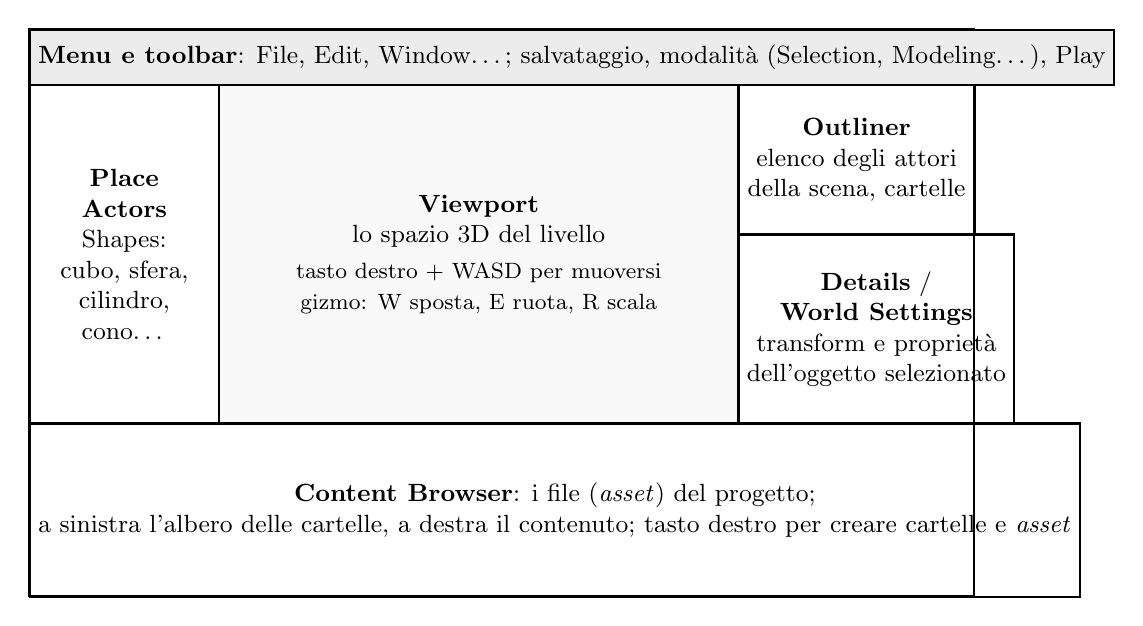
\begin{tikzpicture}[
  font=\small,
  ue1pan/.style={draw, thick, align=center, inner sep=3pt},
  ue1note/.style={font=\footnotesize, align=left, text width=3.4cm}
]
  % cornice
  \draw[thick] (0,0) rectangle (12,7.2);
  % toolbar
  \node[ue1pan, minimum width=12cm, minimum height=0.7cm, anchor=north west, fill=gray!15]
    at (0,7.2) {\textbf{Menu e toolbar}: File, Edit, Window\ldots; salvataggio, modalità
    (Selection, Modeling\ldots), Play};
  % place actors
  \node[ue1pan, minimum width=2.4cm, minimum height=4.3cm, anchor=north west]
    at (0,6.5) {\textbf{Place}\\\textbf{Actors}\\Shapes:\\cubo, sfera,\\cilindro,\\cono\ldots};
  % viewport
  \node[ue1pan, minimum width=6.6cm, minimum height=4.3cm, anchor=north west, fill=gray!5]
    at (2.4,6.5) {\textbf{Viewport}\\lo spazio 3D del livello\\[2pt]
    \footnotesize tasto destro + WASD per muoversi\\\footnotesize gizmo:
    W sposta, E ruota, R scala};
  % outliner
  \node[ue1pan, minimum width=3cm, minimum height=1.9cm, anchor=north west]
    at (9,6.5) {\textbf{Outliner}\\elenco degli attori\\della scena, cartelle};
  % details
  \node[ue1pan, minimum width=3cm, minimum height=2.4cm, anchor=north west]
    at (9,4.6) {\textbf{Details} /\\\textbf{World Settings}\\transform e proprietà\\
    dell'oggetto selezionato};
  % content browser
  \node[ue1pan, minimum width=12cm, minimum height=2.2cm, anchor=north west]
    at (0,2.2) {\textbf{Content Browser}: i file (\emph{asset}) del progetto;\\
    a sinistra l'albero delle cartelle, a destra il contenuto; tasto destro per creare
    cartelle e \emph{asset}};
\end{tikzpicture}
\caption{Una disposizione tipica dell'editor, come quella mostrata da Igor. Ogni pannello
si può spostare, agganciare ad altri o chiudere; il menu Window li riapre.}
\label{ue1:fig:editor}
\end{figure}

\paragraph{Le cartelle, e i loro colori.} Nel Content Browser, con il \textbf{tasto
destro}, si possono creare vari tipi di \emph{asset}; per cominciare, una cartella:
\textbf{New Folder}, chiamata ``prova''. Si possono creare tutte le cartelle che si
vogliono, ``in modo da avere ordine''. Una ``piccola chicchetta'': con il tasto destro
su una cartella, \textbf{Set Color}, la si può \textbf{colorare} (Igor la fa blu), un
feedback visivo che rende la navigazione molto più veloce. Il Content Browser mostra le
cartelle in due modi: a destra come in un \emph{explorer}, a sinistra come un albero ``a
cascata''. Se si mette una cartella dentro un'altra, a sinistra compare una piccola
freccia che apre la cartella sottostante: cartelle e sottocartelle.

\paragraph{L'ordine, per sé e per gli altri.} ``È molto importante l'organizzazione.'' Le
cartelle si riempiranno di \emph{asset}, e bisognerà cercarne uno solo senza sapere dove
andare. L'ordine serve ``non solo per la salvezza vostra, ma anche dei vostri possibili
collaboratori'': ``vi assicuro che quando siete ordinati, la gente vi ringrazia''.

\paragraph{Approfondimento: il Content Drawer e la definizione di \emph{asset}.} Nella
disposizione predefinita di Unreal Engine 5 il Content Browser non è sempre aperto: lo si
richiama dal pulsante \textbf{Content Drawer} in basso a sinistra (o con
Ctrl+Spazio), e lo si può agganciare stabilmente all'interfaccia (``Dock in Layout''),
come ha fatto Igor. Romero e Sewell definiscono l'\emph{asset} come ``un pezzo di
contenuto di un progetto Unreal'': materiali, \emph{static mesh} e Blueprint sono tutti
\emph{asset}. Quando si trascina un \emph{asset} dal Content Browser nel livello,
l'editor ne crea una \textbf{copia} da piazzare nella scena: l'\emph{asset} resta uno, le
sue istanze nel livello possono essere molte. Gli stessi autori descrivono l'Outliner
come l'elenco degli oggetti presenti nel livello, e i Details come il pannello che
mostra le proprietà modificabili dell'oggetto selezionato.

% ---------------------------------------------------------------------
\section{Il primo cubo e il \emph{transform}}
\label{ue1:sec:transform}

\paragraph{Place Actors.} Gli \emph{actor} sono gli elementi di gioco. Dal pannello
\textbf{Place Actors} (se manca: Window, Place Actors), nella sezione \textbf{Shapes},
si prende un \textbf{cubo} e lo si trascina nella viewport. ``Ecco a voi un cubetto
renderizzato'': il primo cubo in Unreal, ``e ne avrete tanti''.

\paragraph{I tre assi.} Sul cubo compaiono tre frecce: sono i tre assi principali,
\textbf{X}, \textbf{Y} e \textbf{Z}, lungo i quali lo si può muovere. Ogni asse ha il
suo colore: \textbf{X rosso}, \textbf{Y verde}, \textbf{Z blu}.

\paragraph{Il \emph{transform}.} Di ogni oggetto si possono modificare
\textbf{locazione}, \textbf{rotazione} e \textbf{scala}. L'insieme dei tre è il
\textbf{\emph{transform}} (``quando parleremo di \emph{transform}, ricordatevelo''), e
lo si rivedrà ``a oltranza''. Lo si modifica in due modi: con le frecce nella viewport,
o con i numeri nel pannello \textbf{Details}.

\paragraph{I numeri nei Details.} Nei Details la locazione del cubo è, per esempio, 480,
430, 120: è la \textbf{raffigurazione numerica}, in unità di Unreal, del punto in cui si
trova l'oggetto. Se si scrive 0 al posto del primo valore e si preme Invio, ``poplà'':
la coordinata X del cubo adesso è 0. Se si trascina una freccia guardando i numeri, si
vede il valore crescere o diminuire, andare in positivo o in negativo: è il verso
dell'asse.

\paragraph{Unreal ragiona in centimetri.} ``Molto importante'': \textbf{l'unità di Unreal
è il centimetro}. Se un oggetto va spostato di tre metri, lo si sposta di 300 unità.
Nella griglia del pavimento ogni riquadro, dice Igor, è un metro, e un cubo, di
default, è un metro.

\paragraph{W, E, R.} Il \textbf{pivot} (o \emph{gizmo}) è ``questo cosettino degli
assi'', e permette tre movimenti: con \textbf{W} si sposta (locazione), con \textbf{E} si
ruota, con \textbf{R} si scala. Gli stessi tre strumenti sono anche in alto a destra
nella viewport, come icone.

\paragraph{Assi locali e assi globali.} Esistono due riferimenti: gli assi
\textbf{relativi} all'oggetto stesso (\textbf{locali}) e quelli del \textbf{mondo}
(\textbf{globali}, la sua \emph{absolute location}). Finché il cubo non è ruotato la
differenza non si vede; ma se lo si ruota fino a farlo diventare ``una specie di rombo''
e si infila nel terreno, alzarlo lungo i suoi assi locali richiede ``un doppio
movimento, così e così'', perché gli assi locali ruotano insieme a lui (``avremo il
nostro bel pivot ruotato di 40 gradi''). Con gli assi globali, invece, l'alto è sempre
l'alto. Il passaggio dall'uno all'altro si fa con l'icona in alto nella viewport:
\textbf{il cubetto con tre assi} indica il riferimento \textbf{locale}, \textbf{il
mondo} indica quello \textbf{globale}. La scelta vale per locazione e rotazione.

\paragraph{La scala è solo locale.} Non vale per la scala: \textbf{un oggetto si può
scalare solo nei suoi assi locali}. Se si scalasse un oggetto ruotato lungo gli assi del
mondo, ``verrebbe totalmente stretchato malissimo'': l'oggetto è girato in un modo e
l'asse in un altro, e allungarlo così lo deformerebbe. Unreal ``ce lo impedisce''.

\paragraph{Le unità di misura del \emph{transform}.} La locazione è in centimetri, la
\textbf{rotazione in gradi} (``io l'ho ruotato e c'è un 40''), la \textbf{scala in
unità}: 1 è la dimensione originale, 2 il doppio.

\begin{figure}[htbp]
\centering
\begin{tikzpicture}[
  font=\small,
  ue1ax/.style={-{Stealth[length=3mm]}, very thick},
  ue1box/.style={draw, thick, rounded corners=3pt, text width=3.6cm, align=left,
               inner sep=5pt}
]
  % assi
  \coordinate (o) at (0,0);
  \draw[ue1ax, red!75!black] (o) -- (2.2,0) node[right]{X};
  \draw[ue1ax, green!50!black] (o) -- (1.2,1.1) node[above right]{Y};
  \draw[ue1ax, blue!75!black] (o) -- (0,2.2) node[above]{Z};
  \fill (o) circle (2pt);
  \node[below=0.2cm of o, font=\footnotesize, align=center]
    {pivot: X rosso, Y verde, Z blu};
  % riquadri
  \node[ue1box, right=2.8cm of o, yshift=1.6cm] (loc)
    {\textbf{Location} (\textbf{W})\\in centimetri\\locale o globale};
  \node[ue1box, below=0.25cm of loc] (rot)
    {\textbf{Rotation} (\textbf{E})\\in gradi\\locale o globale};
  \node[ue1box, below=0.25cm of rot] (sca)
    {\textbf{Scale} (\textbf{R})\\in unità (1 = originale)\\solo locale};
  \node[draw, thick, dashed, fit=(loc)(rot)(sca), inner sep=6pt,
    label={[font=\small\bfseries]above:Transform}] {};
\end{tikzpicture}
\caption{Gli assi e il \emph{transform}. Lo \emph{snapping} (sezione
\ref{ue1:sec:snap}) si imposta separatamente per ognuna delle tre componenti.}
\label{ue1:fig:transform}
\end{figure}

\paragraph{Il tasto Fine.} Un'altra ``piccola chicchetta'': se si piazza un cubo in
aria e si preme il tasto \textbf{Fine} (\emph{End}, quello ``sopra le frecce''), il cubo
cade sulla prima superficie che trova sotto di sé. ``Molto utile'', perché evita di
stare lì ad abbassarlo a occhio.

\paragraph{I Details seguono la selezione.} Ogni volta che si clicca un oggetto, i Details
mostrano \emph{quell'}oggetto: due cubi hanno due locazioni, due rotazioni, due scale.
\textbf{Per modificare i parametri di un oggetto, bisogna selezionarlo.}

\paragraph{Lavorare con i numeri.} I numeri dei Details sono lo strumento preciso, e
sono molto usati, per esempio, dai level designer: ``dobbiamo allargare il corridoio di
tre metri''. Igor allunga un cubo di tre metri sull'asse Y. Nei campi numerici si può
anche scrivere, oppure \textbf{trascinare}: si mette il mouse sul campo e lo si fa
scorrere a destra e a sinistra (``slidando'') per cambiare il valore, su qualunque asse,
per locazione, rotazione e scala.

\paragraph{Reset.} Accanto a ogni gruppo di valori c'è una \textbf{freccetta}: cliccandola,
il valore torna a quello originale (la scala torna a 1, la locazione al punto di
partenza).

% ---------------------------------------------------------------------
\section{Muoversi, duplicare, raggruppare}
\label{ue1:sec:navigazione}

\paragraph{Forme e pivot.} Si possono piazzare tanti \emph{actor} diversi: cilindri,
coni, sfere. Il pivot è al \textbf{centro} di ogni figura, e per questo un cilindro,
appena piazzato, è ``mezzo interrato''. Per \textbf{scalare su tutti gli assi
insieme} si prende il centro del gizmo di scala e si trascina verso l'esterno (allarga)
o verso l'interno (stringe); trascinando una sola maniglia si scala su un solo asse.

\paragraph{Duplicare con Alt.} Igor costruisce un tavolino con un cilindro schiacciato e
uno allungato. Serve un altro pezzo uguale: bisogna prendere un altro cilindro e rifare
tutto? No: \textbf{si tiene premuto Alt e si trascina} (o si ruota) l'oggetto, e se ne
crea una copia esatta. ``Lo userete a manetta.'' Funzionano anche \textbf{Ctrl+C} e
\textbf{Ctrl+V}. Una studentessa, abituata a Blender, si confonde: premeva Alt e lo
lasciava. Alt va \textbf{tenuto premuto mentre si trascina}, ``non è solo \emph{tap}
Alt''.

\paragraph{Muoversi nella viewport.} ``Mi sono dimenticato di dirvelo, perdonatemi'':
per muoversi nella viewport si tiene premuto il \textbf{tasto destro} del mouse e si
usano \textbf{W, A, S, D}, come in un gioco in prima persona; muovendo il mouse si
ruota la camera. Uno studente scopre da solo che \textbf{E} sale e \textbf{Q} scende:
``bravissimo, esatto''. Bisogna cliccare dentro la viewport: è la camera dell'editor,
non quella del gioco.

\paragraph{Seguire un oggetto.} Se si tiene premuto \textbf{Shift} mentre si trascina un
oggetto, la camera lo \textbf{segue} nel movimento: utile per piazzamenti
particolari.

\paragraph{Selezionare più oggetti.} Per selezionare più oggetti si tiene premuto
\textbf{Shift} (o Ctrl) e si cliccano uno dopo l'altro. Con il palo e il piano del
tavolo selezionati, Alt e trascinamento: ``pac!'', un secondo tavolino.

\paragraph{I gruppi.} Selezionare ogni volta tutti i pezzi è scomodo, perché se si
clicca il piano del tavolo si seleziona solo il piano. Si possono allora
\textbf{raggruppare}: si selezionano gli oggetti, tasto destro, \textbf{Group}, oppure
\textbf{Ctrl+G}. Intorno al gruppo compare ``una specie di reticolo verde'', e cliccando
un pezzo qualunque si seleziona il tutto. Si possono anche raggruppare dei gruppi, per
farne uno più grande. Per \textbf{sciogliere} un gruppo: \textbf{Shift+G}, oppure tasto
destro, Groups, \textbf{Ungroup}.

\paragraph{Ctrl+Z.} ``Qua funziona'': \textbf{Ctrl+Z} annulla. ``Sappiatelo, ogni
errore può essere cancellato, o almeno per poco.''

\paragraph{I gruppi non sono un oggetto unico.} Igor fa vedere un limite: se si
\textbf{scala} un gruppo, Unreal non lo scala come un oggetto unico; ogni pezzo si
scala rispettando i propri assi relativi. Per avere un oggetto davvero unico bisognerà
creare una \textbf{static mesh}, ``che vedremo in seguito''.

\paragraph{Mesh e static mesh.} Una \textbf{mesh} è un oggetto solido formato da
poligoni: quando qualcuno dice ``mi serve la mesh del tavolo'' intende il
\textbf{modello 3D} del tavolo. La \textbf{static mesh} è un tipo di mesh; esistono anche
le \textbf{dynamic mesh}, ``un discorso che vedremo più avanti''.

\paragraph{Approfondimento: \emph{transform} relativi nei Blueprint.} Il comportamento dei
gruppi anticipa un tema che nei Blueprint tornerà spesso. Romero e Sewell, nel capitolo
sui nodi matematici, distinguono il \textbf{\emph{transform} del mondo} di un attore
(la sua posizione assoluta nel livello) dal \textbf{\emph{transform} relativo} dei suoi
componenti, che è relativo al componente ``genitore''. Il loro esempio è un tavolo con
sopra una statua: se si sposta il tavolo, la statua lo segue; se si cambia il
\emph{transform} relativo della statua, il tavolo resta dov'è. È il modo in cui, dentro
una Blueprint Class, si costruiscono oggetti composti che si muovono come un tutt'uno.

% ---------------------------------------------------------------------
\section{Lo \emph{snapping} e la velocità della camera}
\label{ue1:sec:snap}

\paragraph{Lo \emph{snapping}.} Ruotando un oggetto, l'editor mostra un numero che sale
a scatti: 20, 30, 40, 50, 60, 70 gradi. È lo \textbf{\emph{snap}}, che si controlla in
alto a destra nella viewport: ci sono tre pulsanti, per locazione, rotazione e scala,
ognuno con un valore. \textbf{Se il pulsante è azzurro, lo \emph{snap} è attivo.}
\begin{itemize}
  \item Senza \emph{snap} di rotazione l'oggetto ruota liberamente, con i decimali; con
        lo \emph{snap} a 10, ruota di dieci gradi alla volta. Cliccando sul numero si
        sceglie il passo: 5, 10, 15, 30, 45, 60, 90, 120 gradi. Con 120, ``pam!'',
        diretto da 0 a 120; con 5, una rotazione più fine.
  \item Lo stesso vale per la \textbf{locazione}: con lo \emph{snap} l'oggetto si muove
        ``a scattini'' (di 1, 5, 10, 50 unità\ldots), senza si muove di qualunque
        valore, decimali compresi.
  \item E per la \textbf{scala}: senza \emph{snap} si scala ``quanto mi pare'', con lo
        \emph{snap} a passi anche molto piccoli, come 0,25.
\end{itemize}
Se lo \emph{snapping} impedisce di mettere un pezzo dove si vuole, ``basta
disattivarlo''.

\paragraph{La velocità della camera.} Per raggiungere ``quella montagna là'' si può
\textbf{velocizzare la camera}: mentre ci si muove (tasto destro premuto), si gira la
\textbf{rotellina del mouse} in avanti per andare più veloci e indietro per andare più
lenti, quando bisogna osservare un oggetto da vicino con precisione (Igor scende fino a
una velocità di 0,03 per guardare sotto il tavolino).

% ---------------------------------------------------------------------
\section{L'Outliner e l'ordine della scena}
\label{ue1:sec:outliner}

\paragraph{L'elenco della scena.} L'\textbf{Outliner} (se manca: Window, Outliner) è una
raffigurazione a lista di \textbf{tutti gli oggetti in scena}. Se si duplica un cono,
nell'Outliner compaiono Cone, Cone2, Cone3, Cone4\ldots{} Un oggetto si può selezionare
sia nella viewport sia nell'Outliner, ed è utile quando ``avete un bel \emph{pack} di
roba'' da gestire. Per eliminare un oggetto: \textbf{Canc} (\emph{Delete}).

\paragraph{Le cartelle dell'Outliner.} Anche nell'Outliner si possono creare cartelle, e
a Igor ``aiuta molto'' nella pianificazione e nel piazzamento. Tasto destro
nell'Outliner, \textbf{Create Folder}, e si crea una cartella ``Coni''. Poi si
selezionano i coni: visto che sono elencati per nome, si clicca il primo, si tiene
premuto \textbf{Shift} e si clicca l'ultimo, e si seleziona tutta la lista; si
trascinano dentro la cartella. Da quel momento, invece di cliccarli uno per uno, basta
il tasto destro sulla cartella e \textbf{Select All Descendants}: ``eccoli qua''.

\paragraph{Perché farlo subito.} ``Immaginatevi una scena intera, gigantesca.'' Senza
ordine si passano ``tre quarti d'ora'' a cliccare un oggetto dopo l'altro; con le
cartelle, un tasto e si è fatto. ``Vi risparmiate molto tempo.''

\paragraph{Il tasto G.} Un ultimo tasto, che Igor spiega durante la dimostrazione: se il
pivot ``scompare'', bisogna premere \textbf{G}. G passa dalla visualizzazione
dell'editor, con gli aiuti visivi, a quella ``normale'' del mondo di gioco, in cui gli
aiuti sono nascosti.

\paragraph{Approfondimento: la Game View.} Il comando si chiama \textbf{Game View}: con G
la viewport mostra la scena come la vedrebbe il giocatore, nascondendo icone,
\emph{gizmo} e oggetti che nel gioco sono invisibili (le icone delle luci, i volumi, i
punti di partenza del giocatore). È comodo per giudicare l'aspetto finale di una scena;
ma se lo si attiva per sbaglio sembra che gli strumenti siano spariti, ed è per questo
che Igor lo nomina proprio quando il pivot ``scompare''.

\begin{table}[htbp]
\centering
\small
\begin{tabular}{@{}p{4.3cm}p{8.7cm}@{}}
\toprule
\textbf{Comando} & \textbf{Che cosa fa} \\
\midrule
Tasto destro + W A S D & muoversi nella viewport; con il mouse si ruota la camera \\
Tasto destro + E / Q & salire / scendere \\
Rotellina (durante il movimento) & velocità della camera: avanti più veloce, indietro
  più lenta \\
W / E / R & gizmo di locazione / rotazione / scala \\
Icona cubetto / mondo & assi locali / globali (per locazione e rotazione) \\
Pulsanti azzurri dello \emph{snap} & attivano lo \emph{snapping} e ne scelgono il
  passo \\
Fine (\emph{End}) & fa cadere l'oggetto sulla superficie sottostante \\
Alt + trascinamento & duplica l'oggetto (Alt tenuto premuto) \\
Ctrl+C / Ctrl+V & copia e incolla \\
Shift + clic & selezione multipla; nell'Outliner, selezione di un intervallo \\
Shift + trascinamento & la camera segue l'oggetto \\
Ctrl+G / Shift+G & raggruppa / separa (anche: tasto destro, Groups) \\
Ctrl+Z & annulla \\
Canc (\emph{Delete}) & elimina l'oggetto selezionato \\
G & Game View: mostra o nasconde gli aiuti dell'editor \\
Freccetta accanto ai valori & riporta il valore all'originale \\
Ctrl+S & salva \\
\bottomrule
\end{tabular}
\caption{I comandi della prima lezione. Tutti valgono nel Level Editor di Unreal Engine
5.5 con le impostazioni predefinite.}
\label{ue1:tab:comandi}
\end{table}

% ---------------------------------------------------------------------
\section{Esercitazione: il ristorante dei tre tavoli}
\label{ue1:sec:esercitazione}

Con quello che si è imparato, ``una piccola esercitazione''. Bisogna costruire, con le
forme di base, \textbf{tre tavoli con le loro sedie}:
\begin{enumerate}
  \item un tavolo con \textbf{tre posti}: ``vengono tre ospiti a cena'';
  \item un \textbf{tavolo quadrato} per \textbf{cinque ospiti};
  \item una \textbf{cena romantica}: un tavolo per \textbf{due}, ``e se volete
        metteteci pure la candela''.
\end{enumerate}
Non serve una sedia precisa: ``l'importante è che applicate tutto quello che abbiamo
fatto''. Chi non riesce oggi può farlo per la volta successiva (``assolutamente''), e
riguardare la registrazione.

\paragraph{Partire da una reference.} Un consiglio, ``soprattutto per voi artisti'': per
fare qualcosa di artistico, prendere una \textbf{reference}. Ma non una sedia troppo
complessa: ``non ci interessa fare una cosa bella e bellissima''. Igor sceglie una
sedia ``molto semplice'', la ``sedia della nonna che vi fa il ragù''.

\paragraph{La dimostrazione.} Igor costruisce la sua sedia passo per passo, ed è un buon
riassunto di tutta la seconda parte:
\begin{enumerate}
  \item un cubo, scalato con lo \emph{snap} a 0,25, per la seduta; la freccetta di reset
        per riportarlo alle dimensioni di partenza quando serve (``le sedie sono alte
        più o meno un metro'');
  \item la prima gamba, posizionata (``se avete problemi con lo \emph{snapping}, basta
        disattivarlo'');
  \item le altre gambe: Shift per selezionare, Alt per duplicare. Ne viene ``questo
        bellissimo sgabello'', con le gambe ``non proprio precisissime'';
  \item lo schienale, duplicando altri pezzi per il dorso;
  \item tutti i pezzi selezionati e \textbf{Ctrl+G}, ``perché sennò dobbiamo fare ogni
        volta uno, due, tre, quattro'';
  \item la sedia accostata al tavolo (``è un po' spesso questo tavolo, ci saranno delle
        ginocchiate incredibili, ma non ci importa'').
\end{enumerate}

\paragraph{Si può allineare un oggetto a un altro?} Uno studente, che oggi può solo
guardare, chiede se c'è un modo di allineare le gambe della sedia a un oggetto, visto
che a mano non è semplice. Igor risponde che non è una cosa che in Unreal si fa
``professionalmente'': strumenti di allineamento precisi ci sono nei programmi di
modellazione, come Blender e Maya. In Unreal ci sono il tasto \textbf{Fine}, lo
\emph{snapping}, il lavoro ``un po' a mano'', i \emph{plugin}, oppure la
\textbf{Modeling Mode}, la modalità di modellazione dell'editor, con strumenti più
precisi, che si vedrà in seguito.

\paragraph{Gli strumenti si somigliano.} Lo stesso studente nota che, in attesa del
download, ha usato \textbf{Inkarnate}, un programma per disegnare mappe, e che i
principi visti finora sono ``molto simili''. ``Sì, assolutamente'': sono principi
condivisi dai vari game engine e dai programmi grafici. In Unity ``magari qualche
bottone è un po' diverso'', ma le funzioni sono simili; ``si impara a muoversi da una
parte e si impara a muoversi dall'altra''. Igor mostra anche \textbf{Dungeon
Scrawl}\footnote{Igor ci arriva per tentativi: ``Dungeon Crawler'', ``Dungeon
Designer'', ``Dungeon Scroll''.}, uno strumento per disegnare mappe per le partite di
D\&D con gli amici, usato anche per il level design.

\paragraph{I risultati.} Dopo una ventina di minuti di lavoro individuale, i
``ristoratori in erba'' mostrano i loro tavoli.
\begin{itemize}
  \item Uno studente ha aggiunto una \textbf{luce} per la candela, ma la candela fa
        ombra. Igor gli mostra come risolvere: si seleziona la luce e nei Details, in
        basso, si toglie la spunta a \textbf{Cast Shadows}.
  \item Qualcuno ha fatto un tavolo rettangolare invece che quadrato: ``va benissimo,
        tranquilli''.
  \item Uno studente, che ha appena finito il download, ha fatto solo la base del tavolo
        e una gamba della sedia, sottilissima. Igor ricorda che Unreal lavora in
        centimetri, e quella gamba è di pochi centimetri: ``non ci farei sedere
        nessuno, potrebbe crollare''. Ma ``è soggettivo''.
\end{itemize}
``A parte l'ironia'', la conclusione è che gli oggetti in sé contano poco: conta capire
come ci si muove in Unreal, duplicando, scalando, muovendo, ruotando. ``Questa è la cosa
più importante che oggi impariamo.''

\paragraph{Una cartella per ogni tavolo.} Un'ultima richiesta: mettere ogni gruppo in una
cartella dell'Outliner. Create Folder, ``Tavolo da due'', si selezionano i pezzi e li si
trascina dentro; poi ``Tavolo da tre'', e così via. Con Select All Descendants si
riprende il tavolo intero in un clic.

% ---------------------------------------------------------------------
\section{Salvare la mappa, e la chiusura}
\label{ue1:sec:chiusura}

\paragraph{Salvare.} Per salvare il lavoro c'è il classico \textbf{Ctrl+S}. Siccome la
mappa è stata creata ``da nulla'', la prima volta Unreal chiede dove salvarla: le si dà
un nome (``MappaProva'') e la si salva dentro la cartella ``prova'' del Content
Browser. In basso a destra, poi, l'editor tiene il conto delle modifiche non salvate:
se si sposta anche solo una sedia, compare l'indicazione degli oggetti
\textbf{\emph{unsaved}}, ``tutti gli oggetti che devo salvare''.

\paragraph{Che cos'è il secondo file?} Uno studente nota che il salvataggio crea anche un
secondo file, un \textbf{HLOD Layer}\footnote{Nella trascrizione ``Halodle'' e ``Halod
Layer''.}. Igor spiega che dipende dalla mappa: quella su cui hanno lavorato contiene un
\textbf{landscape}, le montagne che si vedono in fondo. Il landscape è un piano che si
può modellare con uno strumento apposito per formare, per esempio, il paesaggio di
sfondo; il file salva come quel piano è composto. La volta successiva si userà una
mappa davvero vuota, senza landscape.

\paragraph{Approfondimento: LOD e HLOD.} \textbf{LOD} sta per \emph{level of detail}:
lo stesso oggetto esiste in più versioni, con un numero decrescente di poligoni, e
l'engine usa quelle più semplici quando l'oggetto è lontano dalla camera, dove i
dettagli non si vedrebbero comunque. È la risposta pratica al compromesso della
sezione~\ref{ue1:sec:rendering} tra precisione e peso. Gli \textbf{HLOD}
(\emph{hierarchical} LOD) fanno lo stesso a livello di gruppi: interi blocchi lontani
della mappa vengono sostituiti da un'unica versione semplificata. Le mappe ``a mondo
aperto'' di Unreal Engine 5, con il landscape, li usano per impostazione predefinita, ed
è per questo che il salvataggio crea un file di \emph{HLOD Layer}.

\paragraph{Le ultime domande.} Come si separano gli oggetti raggruppati? ``Shift+G, oppure
tasto destro, Ungroup: se lo cerchi c'è proprio scritto.'' Quando arriva la
registrazione? Sul sito, ``credo il giorno dopo''. Le foto dei lavori si possono mandare
a Igor su Discord, ``tranquillamente'' (``quando ci sono, vi rispondo''), anzi in un
\emph{thread} o un canale apposito, ``così almeno è più ordinato e non mi riempite la
casella privata''.

\paragraph{Il calendario.} Giovedì si rivede Igor; il martedì successivo c'è Davide, con
la parte artistica; poi le lezioni si alternano, ``settimana a settimana''. Sono le 19:
``per chi tra poco cena, auguro buona cena a tutti''. ``Se avete domande, fatele adesso o
tacete fino alla prossima volta.'' ``Ciao, ragazzi.''

% ---------------------------------------------------------------------
\section*{Punti chiave del capitolo}
\addcontentsline{toc}{section}{Punti chiave del capitolo}

\begin{itemize}
  \item Il \textbf{game engine} è ``il calderone'' che riunisce 3D art, programmazione e
        design in un unico ambiente, con fisica e collisioni, suono, animazione,
        networking e IA. Lo si governa con lo \textbf{scripting}; in Unreal, con i
        \textbf{Blueprint}, un linguaggio a nodi usato anche dai programmatori (il C++
        resta per ottimizzare). Conta la \textbf{logica}, più dello strumento.
  \item Il \textbf{rendering} trasforma poligoni in pixel: \textbf{\emph{vertex
        shading}} (i vertici dei triangoli), \textbf{rasterizzazione} (quali pixel),
        \textbf{\emph{fragment shading}} (colore, luce, ombre, riflessi). Più poligoni
        = più precisione, ma più peso: ``un cubo con due milioni di poligoni'' fa
        esplodere il gioco.
  \item Il \textbf{\emph{real time rendering}} lavora tra 20 e 120 \emph{fps}: il cinema
        è a 24, il gaming a 30--60 e oltre. Un \textbf{frame} è un'immagine; la loro
        successione dà l'illusione del movimento.
  \item Unreal è il più usato perché è un \textbf{linguaggio comune}, aggiornato di
        continuo, e perché permette di \textbf{prototipare} subito: ``non ci interessa
        se è bello o brutto, è importante che funzioni'' (il prototipo di
        \emph{Expedition 33}). È usato anche nel cinema, dove conta il dettaglio più
        dell'ottimizzazione.
  \item Ciò che distingue un videogioco da un video è il \textbf{game loop}: input,
        \emph{update}, render, e di nuovo, a ogni \emph{frame}.
  \item \textbf{Ogni buona idea non esiste finché non sta su carta.} Indie, AA e AAA si
        distinguono per i soldi e per la specializzazione dei ruoli (fino ai \emph{leaf
        artist}). L'\textbf{\emph{outsourcing}} è chiedere a un altro studio una parte
        del lavoro, senza cedergli la proprietà.
  \item Tutti i ruoli toccano l'engine: \emph{blockout} e metriche per il level
        designer, momenti scriptati per il narrative designer, parametri esposti per il
        combat designer, materiali e Sequencer per gli artisti, rendering, IA e rete per
        i programmatori, Unreal Insights per il QA. \textbf{Trattate bene i vostri
        programmatori.}
  \item Un gioco è fatto di \textbf{attori, meccaniche, spazio, obiettivi, regole} (e a
        volte \textbf{tempo}); il divertimento è una \textbf{conseguenza}, e il gameplay
        nasce dalle \textbf{scelte}. Meccanica = che cosa posso fare; dinamica = come lo
        faccio; estetica = come mi fa sentire. ``Un gioco per tutti non è un gioco per
        nessuno.''
  \item Il bilanciamento è un lavoro tra \textbf{designer e QA}; il feedback utile è
        quello da cui si ricava un'informazione. Far giocare chi non ha mai visto il
        gioco ``è la cosa più pura''.
  \item Per il corso serve Unreal \textbf{5.5} (la 5.5.4): l'ultimo numero è solo
        l'aggiornamento, il secondo decide la compatibilità.
  \item Le risorse: \textbf{documentazione}, forum, corsi gratuiti di
        \emph{learning}, \textbf{Fab} con i \emph{pack} gratuiti del mese (``prendeteli
        sempre''). Ma \textbf{prima la funzione, poi l'\emph{asset}}, o il progetto
        pesa 70~GB per usarne tre.
  \item Quando si preme Play gli attori vengono inizializzati e duplicati. Ogni
        movimento va reso \textbf{relativo al tempo di gioco} (\emph{delta seconds}),
        altrimenti dipende dagli \emph{fps}.
  \item Il progetto di prova: Games, \textbf{Blank}, Blueprint, Desktop, Starter
        Content, nome \textbf{senza spazi}. I template si distinguono per le
        \textbf{3C}: camera, controller, character.
  \item L'editor è fatto di \textbf{finestre} spostabili (Window le riapre): viewport,
        Details, Outliner, World Settings, \textbf{Content Browser}. Cartelle colorate
        e ordine: ``quando siete ordinati, la gente vi ringrazia''.
  \item Il \textbf{transform} è locazione (\textbf{centimetri}), rotazione
        (\textbf{gradi}) e scala (\textbf{unità}); \textbf{W, E, R}; X rosso, Y verde,
        Z blu; assi locali o globali, ma \textbf{la scala è solo locale}.
  \item \textbf{Alt + trascinamento} duplica, \textbf{Ctrl+G} raggruppa, \textbf{Fine}
        appoggia a terra, lo \textbf{\emph{snap}} azzurro fa muovere a scatti, la
        \textbf{rotellina} cambia la velocità della camera, \textbf{Select All
        Descendants} riprende un'intera cartella dell'Outliner.
\end{itemize}
